\documentclass[12pt,a4paper,twoside,openrigth]{muthesis} % Default font size and left-justified equations
\usepackage[spanish]{babel}
\usepackage{graphicx, array, blindtext}
\usepackage{booktabs}
 \usepackage{multirow}
 \usepackage{multicol}
\usepackage{fancyhdr}
\usepackage[utf8]{inputenc}
\usepackage{pdfpages,float,multirow}
\usepackage{subfig}
\usepackage{bbm}
\usepackage{emptypage} %Quinta en encabezado de las paginas en blanco
\graphicspath{{Imagenes/}{img/}{4img/}}
%\graphicspath{ {estructurasADN/} }
\usepackage{caption}
\usepackage{pdflscape}
\usepackage[lmargin=3cm,rmargin=2cm,tmargin=3cm,bmargin=3cm]{geometry}
%\usepackage[tmargin=3cm,bmargin=3cm,inner=2.5cm,outer=2.5cm,]{geometry}
\usepackage{float}
\usepackage{colortbl}
\usepackage{listings}
\usepackage{xcolor}
\usepackage{blkarray}
\usepackage{lscape}
\usepackage{csquotes}


\definecolor{codegreen}{rgb}{0,0.6,0}
\definecolor{codegray}{rgb}{0.5,0.5,0.5}
\definecolor{codepurple}{rgb}{0.58,0,0.82}
\definecolor{chestnut}{rgb}{0.8, 0.36, 0.36}
\definecolor{mypink3}{cmyk}{0, 0.7808, 0.4429, 0.1412}
\definecolor{burntorange}{rgb}{0.8, 0.33, 0.0}
\definecolor{chromeyellow}{rgb}{1.0, 0.65, 0.0}
\definecolor{mediumturquoise}{rgb}{0.28, 0.82, 0.8}
\definecolor{junebud}{rgb}{0.74, 0.85, 0.34}
\definecolor{candypink}{rgb}{0.89, 0.44, 0.48}
\definecolor{magnolia}{rgb}{0.97, 0.96, 1.0}
\definecolor{jazzberryjam}{rgb}{0.65, 0.04, 0.37}
\definecolor{glaucous}{rgb}{0.38, 0.51, 0.71}


%Bibliografia

%\usepackage[backend=biber,style=numeric,sorting=nty]{biblatex}
\usepackage[backend=biber,sorting=nty]{biblatex}
\addbibresource{Referencias.bib}



%Para el codigo de python
\usepackage{algorithm}
\usepackage{algpseudocode}
\usepackage{listings}
\usepackage{color, xcolor}

\lstdefinestyle{mystyle}{
    backgroundcolor=\color{magnolia},   
    commentstyle=\color{glaucous},
    keywordstyle=\color{jazzberryjam},
    numberstyle=\tiny\color{codegray},
    stringstyle=\color{codepurple},
    basicstyle= \sffamily\footnotesize,
    breakatwhitespace=false,         
    breaklines=true,                 
    keepspaces=false, 
    captionpos=b,  
    numbersep=1pt,                  
    showspaces=false,                
    showstringspaces=false,
    showtabs=false,                  
    tabsize=2
}
\lstset{style=mystyle}

% Color package and define colors
\usepackage{color} %the base color package
\definecolor{darkblue}{rgb}{0,0,1} %you can define any color this way
% Hyper Reference Formatting
\usepackage{hyperref} %[pagebackref] option links back from the bibliography
\hypersetup{colorlinks,breaklinks,linkcolor=darkblue,urlcolor=darkblue,
anchorcolor=darkblue,citecolor=black}


%=============================================================
% Font Settings
%=============================================================

%usepackage{avant} % Use the Avantgarde font for headings
%\usepackage{mathptmx} % Use the Adobe Times Roman as the default text font together with math symbols
%\usepackage{microtype} % Slightly tweak font spacing for aesthetics 

\setlength{\parindent}{0.0in}
\setlength{\parskip}{0.05in}

\usepackage[T1]{fontenc} % Use 8-bit encoding that has 256 glyphs
\usepackage{calc} % For simpler calculation - used for spacing the index letter headings correctly
\usepackage{textcomp} % Text Companion fonts which provide many text symbols in the TS1 encoding.


%===================================================
% Math Formulas
%===================================================
\usepackage{amsmath,amsthm,amsfonts,amssymb,amscd,mathrsfs}
\spanishdecimal{.}
\theoremstyle{definition}
\newtheorem{defn}{Definición}[section]
\newtheorem{teor}{Teorema}[section]
\newtheorem{lema}{Lema}[section]
\newtheorem{Alg}{Algoritmo}[section]
\newtheorem{corl}{Corolario}[section]
\newtheorem{ejemplo}{Ejemplo}[section]
\newtheorem{obs}{Observación}[section]
\newtheorem{propo}{Proposición}[section]
\usepackage[most]{tcolorbox}
\def\proof{\paragraph{Demostraci\'on:\\}}
\def\endproof{\hfill$\blacksquare$}


%Encabezados y pie de página
\fancyhf{}
\lhead[\nouppercase \leftmark]{Brenda Quintana}
\rhead[Brenda Quintana]{\nouppercase \rightmark}
\lfoot[\thepage]{}
\rfoot[]{\thepage}
\renewcommand{\headrulewidth}{0.5pt}
\renewcommand{\footrulewidth}{0pt}
\fancypagestyle{plain}{
\fancyhf{}
\fancyhead[L]{}
\fancyfoot[R]{\thepage}
\renewcommand{\headrulewidth}{0pt}
\renewcommand{\footrulewidth}{0pt}
}
\pagestyle{fancy}

\setcounter{tocdepth}{1} %Para la númeración de los capitulos en el indice de contenidos

%\usepackage{nopageno}
\begin{document}


\includepdf[pages=-]{Portada.pdf}

%%%%%%%%%%%%%%%%%%%%%%%%%%%%%%%%%%%%%%%%%%%%%%%%%%%%%%
%%%%%%%%% COSAS PROTOCOLO DE LA TESIS %%%%%%%%%%%%%%%%
%%%%%%%%%%%%%%%%%%%%%%%%%%%%%%%%%%%%%%%%%%%%%%%%%%%%%%

\cleardoublepage
\pagenumbering{gobble}
\chapter*{Agradecimientos}

Quiero expresar mi profunda gratitud a todas las personas que contribuyeron a la realización de este trabajo.

En primer lugar, agradezco al Dr. José Ulises Márquez Urbina por su orientación experta y consejos pacientes que fueron fundamentales durante todo el proceso de esta investigación. Agradezco también al Dr. Israel Emmanuel Ambriz Lobato por su unvaluable ayuda en la construcción y la implementación del modelo, así como a la Dra. Graciela María de los Dolores González Farías por su guía experta en el ámbito estadístico.

Quiero reconocer al Centro de Investigaciones en Matemáticas, donde encontré a profesores excepcionales que no solo me inspiraron y fomentaron mi pasión por la ciencia, sino que también me alentaron constantemente a seguir adelante.

A mis padres, Gabriela Silva y Guillermo Quintana, les debo un agradecimiento especial por su inquebrantable apoyo y amor desde mi infancia. Su compromiso y dedicación han sido una fuente inagotable de inspiración para mí. A mi hermano Guillermo A. Quintana, le agradezco sus consejos y orientación, tanto en este trabajo como en la vida en general.

No puedo pasar por alto a mis fieles compañeras, Nyx y Kora, cuya presencia constante y afectuosa durante las largas horas de escritura de esta tesis fueron un bálsamo en momentos de frustración.

A mis queridos amigos, Sara, Zaira, Esaul, Franklyn y Alex, les estoy profundamente agradecido por ser un apoyo emocional fundamental a lo largo de mi trayecto de maestría. su compañía, risas y ánimos me han impulsado a dar lo mejor de mí en todo momento.

Este logro no es solo mío, sino también suyo. Agradezco de corazón por estar a mi lado en este largo y gratificante viaje.



\cleardoublepage
\chapter*{Resumen}

La diabetes, una enfermedad crónica que altera el procesamiento de la glucosa, conlleva graves consecuencias, como enfermedades cardíacas, accidentes cerebrovasculares, daño nervioso, problemas visuales, renales y amputaciones. El creciente número de personas afectadas, particularmente en la población mexicana, es motivo de preocupación. Aunque existen índices establecidos para evaluar el riesgo de resistencia a la insulina, como el HOMA o Matsuda, su estimación hecha con poblaciones caucásicas o predominantemente masculinas limita su utilidad generalizada.

Este estudio presenta un enfoque innovador para estimar el riesgo de resistencia a la insulina, utilizando variables fácilmente accesibles para comunidades de bajos recursos y adaptado específicamente a la población mexicana. Se analizan datos de curvas de glucosa e insulina obtenidas durante la prueba de tolerancia a la glucosa y datos biométricos adicionales. Se emplea un enfoque de análisis de datos funcionales, junto con el concepto de bandas de profundidad desarrollado por López Pintado y Romo \cite{boxplotFun}, y posteriormente trabajado y mejorado por Emmanuel Ambriz en su tesis doctoral, para modelar las dependencias mediante copulas y realizar regresiones mediante técnicas de regresión cuantil.

Se exploran diversos modelos con diferentes conjuntos de variables y secciones de la población (hombres y mujeres), seguidos de una comparación de su desempeño. Este estudio promete proporcionar una herramienta más precisa y personalizada para la evaluación del riesgo de resistencia a la insulina, crucial para la prevención y manejo de la diabetes en la población mexicana.








%%%%%%%%%%%%%%%%%%%%%%%%%%%%%%%%%%%%%%%%%%%%%%%%%%%%%
%%%%%%%%%%% AQUI EMPIEZA LA NUMERACION %%%%%%%%%%%%%%
%%%%%%%%%%%%%%%%%%%%%%%%%%%%%%%%%%%%%%%%%%%%%%%%%%%%%

\cleardoublepage
\setcounter{page}{1}
\pagenumbering{Roman} % para comenzar la numeración de paginas en números romanos
\tableofcontents% indice de contenidos

\addcontentsline{toc}{chapter}{Índice de Figuras} % para que aparezca en el indice de contenidos
\cleardoublepage
\listoffigures % indice de Figuras

%%%%%%%%%%%%%%%%%%%%%%%%%%%%%%%%%%%%%%%%%%%%%%%%%%%%%
%%%%%%%%%%%%%% AQUI EMPIEZA LA TESIS %%%%%%%%%%%%%%%%
%%%%%%%%%%%%%%%%%%%%%%%%%%%%%%%%%%%%%%%%%%%%%%%%%%%%%

\pagenumbering{arabic}
\prefacesection{Introducción}
\markboth{Introducción}{}


La diabetes mellitus es una enfermedad metabólica crónica que representa un desafío de salud pública a nivel mundial. Está caracterizada por mantener los niveles altos de glucosa en sangre, lo cual tiene que ver con la producción de insulina de nuestro cuerpo.A pesar de los avances en el diagnóstico y tratamiento, la prevalencia de la diabetes sigue aumentando, y su impacto en la calidad de vida de los individuos y en los sistemas de salud es significativo. Una de las dificultades en el manejo efectivo de la diabetes radica en la falta de modelos precisos y adaptados a poblaciones específicas, lo que puede llevar a diagnósticos erróneos o a la subestimación del riesgo de desarrollar la enfermedad \cite{HOMAMex}.

De acuerdo con las estadísticas tomadas de la página del Instituto Nacional de Estadística y Geografía (INEGI) del período enero-junio del 2023, en México la diabetes es la segunda causa de muerte \cite{INEGI}. Año con año la tasa de personas con esta enfermedad aumentó súbitamente, lo alarmante de esta situación es que muchas personas en México la padecen y no lo saben. Las causas de esta enfermedad son muy variadas, por ejemplo, malos hábitos alimenticios, línea genética, llevar una vida sedentaria, entre otras \cite{PromoSaludMexico}.

En este contexto, el presente trabajo se enfoca en abordar esta brecha identificando y proponiendo un modelo ajustado específicamente para la población mexicana. Aún cuando existen índices de medición para la resistencia a la insulina, como el índice HOMA o el índice de Matsuda, estos se encuentran calibrados principalmente para poblaciones caucásicas o para individuos en su mayoría hombres. La falta de análisis previos para poblaciones particulares, así como la imposibilidad de incluir individuos representativos de todas las diversidades existentes, resalta la necesidad de desarrollar un modelo específico que considere las características genéticas, ambientales y culturales únicas de la población mexicana.

El objetivo principal de este estudio es proponer un modelo de predicción de la diabetes mellitus tipo 2 que considere las particularidades específicas de la población mexicana, utilizando datos biométricos y clínicos disponibles para cualquier tipo de comunidad. Se espera que este modelo contribuya a mejorar la precisión del diagnóstico, identificar de manera temprana a las personas en riesgo de desarrollar la enfermedad y, en última instancia, facilitar la implementación de intervenciones preventivas y estrategias de manejo personalizadas.

Afortunadamente, en la comunidad mexicana hay varios investigadores comprometidos en encontrar soluciones para esta enfermedad tan prevalente. La Dra. Adriana Monroy Guzmán, en colaboración con el Centro de Investigación en Matemáticas (CIMAT), ha dedicado mucho esfuerzo y dedicación a la recopilación de una base de datos que incluye mediciones de glucosa e insulina durante la prueba oral de tolerancia a la insulina, así como datos adicionales como el índice de masa corporal (IMC), la presión arterial, los porcentajes de grasa, entre otros. Con esta invaluable información y el continuo trabajo del destacado estudiante de doctorado Israel Emmanuel Ambriz Lobato, quien ha investigado ampliamente sobre el uso de cópulas y su implementación en modelos estadísticos, y ha desarrollado un modelo de regresión. Esta investigación ha sido realizada bajo la tutela de la Dra. Graciela González Farías y el Dr. José Ulises Márquez Urbina, con la supervisión médica de la Dra. Monroy.

Cabe destacar que una de las principales motivaciones es lograr una mejor comprensión de las relaciones modeladas en los métodos de Machine Learning y evitar el uso de `cajas negras', es fundamental realizar un análisis estadístico detallado. Este análisis permite verificar si el ajuste del modelo de regresión tiene sentido y está en línea con los conocimientos médicos existentes. Al integrar métodos estadísticos rigurosos, se pueden interpretar los resultados de manera más transparente y confiable, asegurando que las predicciones y conclusiones obtenidas sean válidas y útiles desde una perspectiva clínica.

En el Capítulo \ref{insulina}, se presenta un análisis detallado del proceso de la homeostasis de la glucosa con el objetivo de comprender los factores clave que regulan los niveles de glucosa en la sangre. Además, se aborda el síndrome metabólico, resaltando el proceso de fallo en la síntesis de la insulina y destacando algunas características importantes para identificar este trastorno.

Se describe la prueba oral de tolerancia a la glucosa como una medida para la efectiva de la sensibilidad a la insulina, así como el test de Clamp, considerado el estándar por excelencia para medir la resistencia a la insulina. Sin embargo, debido a su complejidad y carácter invasivo, el test de Clamp rara vez se utiliza en la práctica clínica. Por lo tanto, la comunidad científica ha propuesto varios índices como referencia para evaluar la resistencia a la insulina.

Además, se mencionan diversas aproximaciones que la comunidad científica ha empleado para abordar esta problemática, incluyendo modelado con ecuaciones diferenciales, modelos bayesianos, entre otros enfoques.

En el Capítulo \ref{RegCuanDatosFun}, se introduce el modelo matemático con el que se trabajará, comenzando con la descripción de conceptos fundamentales del área de probabilidad. Se exploran conceptos como el cuantil, las funciones de distribución multivariadas y las funciones de distribución marginales, entre otros, haciendo especial énfasis en su formulación muestral. El objetivo principal de esta sección es sentar las bases para comprender la regresión cuantil, un enfoque estadístico que difiere significativamente de la clásica regresión lineal convencional.

La regresión cuantil presenta varias ventajas, siendo una de las más destacables su robustez ante la presencia de valores atípicos. Además, esta técnica permite realizar la regresión con un cierto nivel de confianza, lo cual facilita la estimación de intervalos de confianza con una determinada fiabilidad. Para ilustrar estas diferencias y ventajas, se presenta un ejemplo que contrasta la regresión cuantil con la regresión lineal tradicional, resaltando cómo la primera puede proporcionar resultados más robustos y útiles en ciertos escenarios.


Como última herramienta fundamental, se introduce el concepto de datos funcionales, que consisten en representar las observaciones como funciones, cuya característica distintiva es que no solo se considera el valor de la variable, sino también su forma y escala. Este enfoque resulta de vital importancia para el presente trabajo, dado que el objetivo principal es modelar la relación entre los niveles de glucosa y de insulina en los pacientes utilizando las mediciones obtenidas durante la prueba de tolerancia a la glucosa oral.

Para lograr esto, se emplea la técnica de las bandas de profundidad, la cual permite crear una variable respuesta escalar que conserva su esencia funcional. Esta variable respuesta puede ser modelada utilizando copulas, una herramienta poderosa en el análisis de dependencia entre variables aleatorias. 

El Capítulo \ref{CapCopulas} se centra en la introducción del concepto de copula y su relación con la función de distribución, explorando además su estimación muestral y algunas técnicas exploratorias para comprender su relación y su modelado paramétrico. El objetivo principal de esta sección es preparar al lector para la presentación de las R-vines, una forma particular de descomponer la distribución en copulas a pares.

Las R-vines tienen la característica de poder ser visualizadas como grafos, lo que facilita su comprensión e interpretación. Aunque existen varias formas de realizar esta descomposición, se optará por la estructura de descomposición D-vine como enfoque central debido a su clara interpretación en la unión de nodos y su estructura de grafo.

El objetivo final de este capítulo es unir el concepto de cópula como modelo con la regresión cuantil como técnica de estimación. De esta manera, una vez explorada la parte matemática, se podrá describir el algoritmo computacional y las herramientas que se utilizarán para construir el modelo de regresión, además de presentar uno de los principales resultados de la tesis: la implementación de la paquetería en R, \textbf{deerVineReg}.


El Capítulo \ref{Resultados} se puede dividir en 2 partes. La primera comienza con un análisis exploratorio de la base de datos para tener una noción de cómo está conformada, haciendo énfasis en las estructuras de las sub-bases determinadas por los diferentes prediagnósticos, y así poder comprender la relación entre insulina y glucosa. Posteriormente, se detalla la construcción e interpretación de los gráficos implementados para la visualización de dependencias en cópulas a pares, cuya idea fue tomada del artículo \textit{Copula-based statistical dependence visualizations}. 

Adicionalmente, se presenta la gráfica de efectos, cuya utilidad es observar cómo varía el estimador cuantil en respuesta a cambios en un predictor específico. Esta herramienta permite identificar la relación y el impacto de cada predictor en el resultado de interés, facilitando la interpretación de los modelos y la toma de decisiones. Finalmente, se culmina con la presentación de la librería \textit{deerVineReg}, destacando sus capacidades y beneficios en la implementación de modelos de cópulas para la predicción de la relación entre insulina y glucosa.

En la segunda parte, se aborda el modelo implementado con toda la población, que consta de cuatro covariables predictoras. Aunque si se desea ver los modelos construidos solo para hombres o mujeres, estos se pueden encontrar en el Apéndice \ref{ApendiceA}. Se discuten las dependencias observadas con los gráficos presentados anteriormente y se evalúa el ajuste del modelo.

A partir de este análisis, se concluye que un modelo con tres variables es el que mejor extrae las características significativas, optimizando así la precisión y la interpretabilidad del modelo. Esto cumple con el objetivo de la tesis, que consiste en desarrollar un modelo específico para la población mexicana, proporcionando una herramienta más adaptada y eficaz para el diagnóstico y manejo de la diabetes en esta población.










\cleardoublepage


\chapter{Síndrome Metabólico}\label{insulina}

La glucosa es la principal fuente de energía para todos los tejidos del cuerpo humano. Es crucial que los niveles de azúcar en la sangre se mantengan dentro de un rango óptimo de 60 a 120 mg/dl para garantizar un suministro adecuado de energía al sistema nervioso y a todo el organismo \cite{ImgHomeos}.

Para regular estos niveles, el cuerpo cuenta con dos hormonas clave: la insulina y el glucagón. La insulina, producida por el páncreas, juega un papel fundamental en la absorción y utilización de la glucosa por parte de las células del cuerpo. Esta hormona controla la velocidad a la que la glucosa se consume en los músculos, el tejido graso y el hígado, permitiendo que las células obtengan la energía necesaria para su funcionamiento adecuado.

Por otro lado, el glucagón, también producido por el páncreas, actúa en sentido contrario a la insulina. Cuando los niveles de glucosa en la sangre son bajos, el glucagón se libera para estimular la liberación de glucosa almacenada en el hígado, asegurando así un suministro constante de energía cuando es necesario.

Es importante destacar que cada célula del cuerpo utiliza la glucosa de manera diferente, y este uso está determinado por el sistema enzimático específico de cada tipo celular. Esta diversidad en la utilización de la glucosa refleja la complejidad del metabolismo humano y la importancia de mantener un equilibrio adecuado en los niveles de azúcar en la sangre para garantizar un funcionamiento óptimo del organismo.\cite{capitulo4Metabolic}
%%%%%%%%%%%%%%%%%%%%%%%%%%%%%%%%%%%%%%%%%%%%%%%%%%%%%%%
%%%%%%%%%%%%%%%%%%%%%%%%%%%%%%%%%%%%%%%%%%%%%%%%%%%%%%%

\section{Homeostasis de la Glucosa}

La homeostasis de la glucosa, esencial para la vida de los mamíferos, es un proceso complejo que garantiza un equilibrio adecuado de azúcar en la sangre en todo momento. Después de ingerir alimentos, durante el proceso digestivo, la glucosa es absorbida y liberada en el plasma sanguíneo. Este aumento en los niveles de glucosa estimula a las células beta del páncreas a secretar una hormona vital llamada insulina \cite{capitulo4Metabolic}.

La insulina desempeña un papel crucial en la regulación de los niveles de glucosa en la sangre. Actúa disminuyendo los niveles de glucosa en los tejidos periféricos, promoviendo la síntesis de glucógeno en el hígado y en los músculos, y reduciendo la lipogénesis hepática. De esta manera, la insulina ayuda a mantener los niveles de glucosa dentro de un rango óptimo para el funcionamiento del organismo.

Durante el estado de ayuno, cuando no se ingieren alimentos, los niveles de glucosa en el plasma se mantienen entre $4$ y $5$ mM gracias a la acción del hígado, que almacena glucosa en forma de glucógeno. En este estado, los niveles de insulina son bajos y el hígado se convierte en la principal fuente de glucosa plasmática. En este contexto, las células alfa del páncreas producen la hormona glucagón, cuya función es elevar los niveles de glucosa en la sangre mediante la degradación de glucógeno \cite{unamHomeostasis}.

El hígado y las células beta del páncreas son los principales reguladores de las concentraciones de insulina y glucosa en el plasma, en la Figura \ref{fig:homeostasis} \footnote{Imagen tomada de \cite{ImgHomeos}} se ilustra el proceso anteriormente mencionad. Sin embargo, el grado de hiperglucemia puede variar dependiendo de la capacidad de las células beta para secretar insulina y del grado de resistencia a la insulina en el organismo.

\begin{figure}[H]
    \centering
    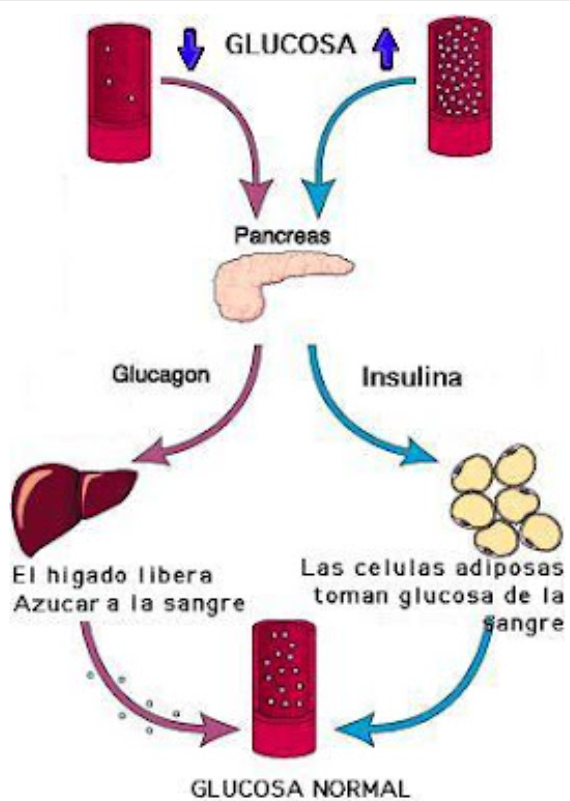
\includegraphics[width = 0.4\textwidth]{homeostasis.png}
    \caption{Esquema General de la Homeostasis de la Glucosa.}
    \label{fig:homeostasis}
\end{figure}

Cuando la homeostasis de la glucosa se ve alterada, se puede desarrollar el síndrome metabólico (SM), un conjunto de condiciones médicas que aumentan el riesgo de desarrollar enfermedades cardiovasculares y diabetes tipo 2. En muchos casos, el SM se presenta cuando las células beta del páncreas se agotan debido a una exposición prolongada a niveles elevados de glucosa en sangre, lo que puede conducir al desarrollo de la diabetes tipo 2. A pesar de los avances en la investigación, este proceso aún no se comprende completamente \cite{capitulo4Metabolic}.

La baja tolerancia a la glucosa en personas sin diabetes se asocia con una respuesta reducida de las células beta a la glucosa, mientras que en personas obesas, esta baja tolerancia se relaciona con una disminución en la sensibilidad a la insulina \cite{computational}. Estas alteraciones en la respuesta metabólica son componentes clave en el desarrollo del síndrome metabólico y la diabetes tipo 2.

Para comprender mejor estos procesos y prevenir las complicaciones asociadas, se han utilizado varios modelos matemáticos para calcular parámetros fisiológicos relacionados con la homeostasis de la glucosa. Estos modelos utilizan datos experimentales para proporcionar una representación matemática precisa de cómo el cuerpo regula los niveles de glucosa en la sangre. Sin embargo, el creciente impacto de la diabetes tipo 2 en la sociedad actual plantea desafíos adicionales, ya que esta enfermedad representa una perturbación significativa en el sistema homeostático de la glucosa \cite{ModelacionMatematica2020}.

%%%%%%%%%%%%%%%%%%%%%%%%%%%%%%%%%%%%%%%%%%%%%%%%%%%%%%%
%%%%%%%%%%%%%%%%%%%%%%%%%%%%%%%%%%%%%%%%%%%%%%%%%%%%%%%%

\section{Resistencia a la Insulina}

La sensibilidad a la insulina y la resistencia a la misma son conceptos fundamentales en el estudio de la fisiopatología de la Diabetes Mellitus (DM). La sensibilidad a la insulina se refiere a la capacidad de los tejidos, especialmente los músculos y los órganos, para responder a la acción de la insulina a través de los receptores de insulina. Por otro lado, la resistencia a la insulina se caracteriza por una disminución en la respuesta de los tejidos a la acción de la insulina, lo que requiere una mayor cantidad de insulina para suprimir la producción de glucosa hepática \cite{MedicionEstimacion}.

En individuos con resistencia a la insulina, se observa una discrepancia entre la concentración de insulina en el plasma y su efectividad para controlar los niveles de glucosa en sangre. En la Diabetes Mellitus, esta resistencia a menudo se presenta junto con altos niveles de glucosa en sangre, lo que puede complicar aún más la regulación de los niveles de azúcar en la sangre.

La causa exacta de la resistencia a la insulina en la DM sigue siendo objeto de debate en la comunidad científica. Se ha sugerido que factores como la obesidad, la inflamación crónica y los factores genéticos pueden contribuir a esta condición. Además, se ha planteado la posibilidad de que la presencia de altos niveles de glucosa en sangre o anticuerpos contra la insulina pueda desempeñar un papel en el desarrollo de la resistencia a la insulina \cite{MedicionEstimacion}.

La Figura \ref{fig:Resistencia}, tomada de \cite{ImgResis}, ilustra este concepto de resistencia a la insulina, mostrando la discrepancia entre los niveles de insulina en el plasma y la respuesta de los tejidos a esta hormona. Esta representación visual ayuda a comprender la complejidad de la relación entre la insulina y la glucosa en el contexto de la Diabetes Mellitus.

\begin{figure}[H]
    \centering
    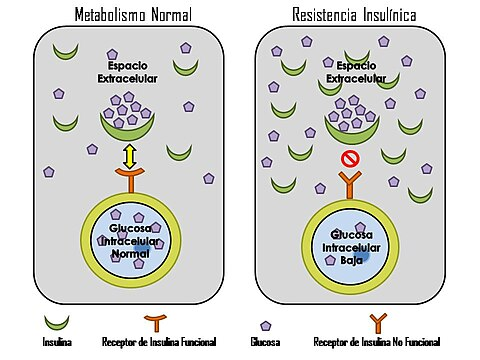
\includegraphics[width = 0.7 \textwidth]{ResisteciaIns.jpg}
    \caption{Resistencia a la Insulina}
    \label{fig:Resistencia}
\end{figure}

Para evaluar la efectividad de la insulina en el organismo, se han desarrollado dos métodos principales: los métodos deducidos y los métodos regresivos. En los métodos deducidos, se utilizan fórmulas derivadas de la lógica y el razonamiento para estimar la sensibilidad a la insulina. Por otro lado, los métodos regresivos proporcionan una fórmula mediante el análisis regresivo de datos experimentales \cite{MedicionEstimacion}.

Una de las pruebas más utilizadas para medir la sensibilidad a la insulina es la prueba de tolerancia a la insulina, también conocida como clamp de insulina. En esta prueba, se administra una cantidad controlada de insulina (0.1 U por kilogramo de peso corporal) y se mide el descenso de la glucosa en el plasma. Sin embargo, este procedimiento puede inducir un estado de hipoglucemia, por lo que se aplica simultáneamente una infusión de glucosa para mantener los niveles de glucosa en sangre en un rango constante. Durante la prueba, se registran los requerimientos de glucosa y la cantidad de insulina necesaria para mantener la homeostasis glucémica. Aunque esta prueba se considera el estándar para medir la sensibilidad a la insulina, su implementación es compleja y se utiliza principalmente en entornos de investigación, no en la práctica clínica de rutina \cite{MedicionEstimacion}.

Dada la complejidad de la prueba de tolerancia a la insulina, se han propuesto otros índices y métodos para evaluar la sensibilidad a la insulina de manera más accesible en entornos clínicos. Estos índices pueden ser útiles para estimar la capacidad del organismo para secretar insulina y para identificar una posible disfunción en el metabolismo de la glucosa.
%%%%%%%%%%%%%%%%%%%%%%%%%%%%%%%%%%%%%%%%%%%%%%%%%%%%%%%

\subsection{Índices de Medición}

Para medir la resistencia a la insulina, se han propuesto varios índices que van desde métodos simples hasta aquellos que toman en cuenta medidas de glucosa e insulina durante pruebas de tolerancia a la glucosa. Algunos de los índices más comúnmente utilizados son el índice HOMA (Homeostasis Model Assessment) o QUICK (Quantitative Insulin Sensitivity Check Index), que se calculan a partir de medidas de glucosa e insulina en sangre en ayunas. Otros índices, como el índice de Matsuda, consideran todas estas concentraciones durante la prueba de tolerancia a la glucosa (OGTT, por sus siglas en inglés) \cite{MedicionEstimacion}.



%%%%%%%%%%%%%%%%%%%%%%%%%%%%%%%%%%%%%%%%%%%%%%%%%%%%%%%

\subsection{Índice HOMA}

El modelo de homeostasis para evaluar la resistencia a la insulina, conocido por sus siglas en inglés como HOMA-IR, es un índice ampliamente utilizado en la investigación para medir la resistencia a la insulina. Fue propuesto por primera vez en 1985 por Rury Holman y David Matthews. Este modelo se basa en la idea de un ciclo de retroalimentación entre las células beta pancreáticas y el hígado.

En el HOMA-IR, la concentración de glucosa en sangre está regulada por la producción de glucosa hepática, mientras que los niveles de insulina en sangre dependen de la respuesta de las células hepáticas a la insulina. Es importante destacar que este índice solo utiliza mediciones de glucosa e insulina en sangre en ayunas. Por lo tanto, una baja respuesta de las células beta a los estímulos de glucosa puede reflejar una deficiencia en la función de estas células, mientras que la resistencia a la insulina se manifiesta como una disminución en la capacidad de la insulina para suprimir la producción de glucosa por parte del hígado \cite{indicesRes}.

El HOMA-IR es una herramienta conveniente y menos invasiva en comparación con el método de clamp de insulina. Se calcula multiplicando la concentración de insulina plasmática en ayunas (FPI) por la concentración de glucosa plasmática en ayunas (FPG), y luego dividiendo el resultado por la constante 22.5, como se muestra en la ecuación:

\begin{equation}\label{HOMAIR}
    HOMA-IR = \frac{FPI \times FPG}{22.5}
\end{equation}

Este índice proporciona una estimación de la resistencia a la insulina y es útil en la investigación clínica y epidemiológica para evaluar el riesgo de diabetes tipo 2 y otras condiciones relacionadas con la resistencia a la insulina.

Además de la evaluación de la resistencia a la insulina mediante el HOMA-IR, también es posible estimar el funcionamiento de las células beta pancreáticas utilizando la ecuación \eqref{HOMAbeta}, conocida como HOMA para las células beta:

\begin{equation}\label{HOMAbeta}
    \text{HOMA células beta} =  20 \times \frac{FPI}{FPG -3,5}
\end{equation}

Esta ecuación proporciona una estimación del funcionamiento de las células beta pancreáticas en relación con los niveles de insulina y glucosa en sangre.

Para interpretar los resultados del HOMA-IR y el HOMA para las células beta, se han establecido valores de referencia. En general, si el valor del HOMA-IR es menor a 1.96, se considera que la sensibilidad a la insulina es adecuada. Si el valor se encuentra entre 1.96 y 2.9, se sospecha de resistencia a la insulina y se pueden requerir estudios adicionales. Finalmente, si el valor es superior a 3, se considera que hay resistencia a la insulina \cite{limiteHOMA}.

Sin embargo, estudios han sugerido que los valores de referencia del HOMA-IR pueden variar entre diferentes poblaciones. Por ejemplo, según el artículo `\textit{The Definition of Insulin Resistance Using HOMA-IR for Americans of Mexican Descent Using Machine Learning}' \cite{HOMAMex}, los valores de referencia para individuos mexicano-americanos son los siguientes: un HOMA-IR menor a 2.6 se considera una sensibilidad normal a la insulina, valores entre 2.6 y 3.8 se consideran en el límite, con posible resistencia a la insulina, y valores superiores a 3.8 indican resistencia a la insulina.

Estas diferencias resaltan la importancia de considerar las características específicas de la población al interpretar los resultados del HOMA-IR y el HOMA para las células beta, y subrayan la necesidad de más investigación para establecer valores de referencia precisos en diferentes grupos étnicos.

%%%%%%%%%%%%%%%%%%%%%%%%%%%%%%%%%%%%%%%%%%%%%%%%%
%%%%%%%%%%% I N D I C E   H O M A  %%%%%%%%%%%%%%
%%%%%%%%%%%%%%%%%%%%%%%%%%%%%%%%%%%%%%%%%%%%%%%%%

\subsection{Índice de Matsuda}

El índice Matsuda de sensibilidad a la insulina ($ISI_{\text{Matsuda}}$) fue propuesto por Matsuda y DeFronzo como una medida de la sensibilidad a la insulina en el organismo. Este índice se calcula utilizando los niveles de glucosa ($mg/dl$) e insulina ($mIU/l$) en sangre tanto en ayunas como durante una prueba de tolerancia a la glucosa oral. La fórmula para calcular el ISI de Matsuda se muestra en la ecuación \eqref{IndexMatsuda}:

\begin{equation}\label{IndexMatsuda}
    ISI_{\textbf{Matsuda}} = \frac{10\;000}{\sqrt{G_0 \times I_0 \times G_{mean} \times I_{mean}}}
\end{equation}

En esta ecuación, $10;000$ es una constante utilizada para obtener un número entre $0$ y $12$, $G_0$ e $I_0$ representan las concentraciones de glucosa e insulina en sangre en ayunas, respectivamente. $G_{\text{mean}}$ es el promedio de las concentraciones de glucosa durante la OGTT, mientras que $I_{\text{mean}}$ es el promedio de las concentraciones de insulina durante la OGTT.

El índice Matsuda de sensibilidad a la insulina tiene un gran poder predictivo para identificar el inicio de la diabetes tipo 2. Al proporcionar una medida de la sensibilidad a la insulina en respuesta a la glucosa, este índice puede ayudar a los médicos a evaluar el riesgo de diabetes tipo 2 en pacientes y a diseñar estrategias de prevención y tratamiento adecuadas \cite{indicesRes}.

%%%%%%%%%%%%%%%%%%%%%%%%%%%%%%%%%%%%%%%%%%%%%%%%%%%%%%%
\subsection{Otros Índices}

Aunque los índices HOMA-IR y Matsuda son ampliamente utilizados en la investigación para evaluar la sensibilidad a la insulina, existen otros índices que también son objeto de estudio. En el artículo "Novel Insulin Sensitivity Index Derived from Oral Glucose Tolerance Test" \cite{NovelInsulin}, se investigó la correlación entre varios índices comúnmente utilizados y la prueba de clamp de insulina, que es considerada el estándar de oro para medir la sensibilidad a la insulina.

En la Tabla \ref{tab:indices} se muestran algunos de estos índices junto con sus respectivas fórmulas. Estos índices fueron evaluados en términos de su capacidad para predecir la sensibilidad a la insulina medida mediante la prueba de clamp de insulina.

\begin{table}[H]
    \centering
    \begin{tabular}{|c|c|}
        \hline \textbf{ Índice } & \textbf{ Ecuación } \\
        \hline \textbf{ HOMA } & $\frac{22.5 \times 18}{I_0  \times G_0}$ \\
        \hline \textbf{ QUICKI } & $\frac{1}{\log (\text { fasting insulin })+\log \text { (fasting glucose) }}$ \\
        \hline \textbf{ Belfiore } & $\frac{2}{(\text { AUC insulin } \times \text { AUC glucose })+1}$ \\
        \hline \textbf{ Cederholm } & $\frac{75,000+(\text { fasting glucose }-2 \text {-h glucose }) \times 1.15 \times 180 \times 0.19 \times \mathrm{BW}}{120 \times \log (\text { mean insulin }) \times \text { mean glucose }}$\\
        \hline \textbf{ Gutt } & $\frac{75,000+(\text { fasting glucose }-2-\mathrm{h} \text { glucose }) \times 0.19 \times \mathrm{BW}}{120 \times \log ([\text { fasting insulin }+2-\mathrm{h} \text { insulin }] / 2) \times[\text { fasting glucose }+2-\mathrm{h} \text { glucose }] / 2}$ \\
        \hline \textbf{ Matsuda } & $\frac{10,000}{\sqrt{(\text { fasting glucose } \times \text { fasting insulin }) \times(\text { mean glucose } \times \text { mean insulin })}}$ \\
        \hline \textbf{ Stumvoll } & $0.22-0.0032 \times \text { BMI }-0.0000645 \times 2 \text {-h insulin }-0.0037 \times 1.5 \text {-h glucose }$ \\
        \hline
    \end{tabular}
    \caption{Índices de Resistencia a la Insulina proveniente de OGTT, tabla tomada de \cite{NovelInsulin}}
    \label{tab:indices}
\end{table}

El artículo \cite{NovelInsulin}, presenta una tabla que muestra los niveles de correlación entre los diferentes índices y la prueba de clamp de insulina. Entre aquellos con mejor desempeño se encuentra el índice Matsuda. Estos resultados ofrecen información importante sobre la utilidad y la precisión de estos índices en comparación con la prueba de clamp de insulina, lo que puede ayudar a los investigadores y clínicos a seleccionar el índice más apropiado para sus estudios o práctica clínica.

Estos índices ofrecen una variedad de enfoques para evaluar la sensibilidad a la insulina y pueden ser útiles en diferentes contextos clínicos y de investigación. Sin embargo, es importante tener en cuenta que cada índice puede tener limitaciones y es crucial validar su utilidad en diferentes poblaciones y condiciones clínicas antes de su aplicación generalizada.


%%%%%%%%%%%%%%%%%%%%%%%%%%%%%%%%%%%%%%%%%%%%%%%%%%%%%%%
%%%%%%%%%%%%%%%%%%%%%%%%%%%%%%%%%%%%%%%%%%%%%%%%%%%%%%%
%%%%%%%%%%%%%%%%%%%%%%%%%%%%%%%%%%%%%%%%%%%%%%%%%%%%%%%

\section{Diabetes}

La Diabetes Mellitus es una enfermedad metabólica crónica que se caracteriza por la presencia de niveles inadecuados de glucosa en sangre. Se han identificado varias subclasificaciones de la enfermedad, que incluyen:

\begin{itemize}
    \item \textbf{Diabetes tipo 1}: Esta forma de diabetes se caracteriza principalmente por la auto destrucción de las células beta del páncreas, típicamente como resultado de un proceso autoinmune. Esto conduce a la destrucción total de las células beta y, por lo tanto, a una deficiencia absoluta de insulina. La diabetes tipo 1 generalmente se presenta durante la niñez o la adolescencia \cite{diabetes}.


    \item \textbf{Diabetes tipo 2}: La diabetes tipo 2 está asociada principalmente con la resistencia a la insulina, una deficiencia relativa de insulina y la presencia de hiperglucemia. Si bien algunos casos de diabetes tipo 2 pueden tener un componente autoinmune, en la mayoría de los casos la enfermedad se desarrolla como resultado de factores como la obesidad y el envejecimiento. Estos factores contribuyen al desgaste en el funcionamiento de las células beta pancreáticas para producir suficiente insulina. La diabetes tipo 2 afecta principalmente a adultos de mediana edad o mayores \cite{computational}.
\end{itemize}

Además de estos dos subtipos principales, existen otras formas de diabetes mellitus, como la diabetes juvenil de inicio en la madurez (MODY), la diabetes gestacional, la diabetes neonatal y la diabetes inducida por esteroides. Sin embargo, este trabajo se enfocará principalmente en el diagnóstico y manejo de la diabetes tipo 1 y tipo 2 debido a su prevalencia y relevancia clínica \cite{diabetes}.

En ambas formas de diabetes mellitus, el cuerpo pierde la capacidad de controlar adecuadamente los niveles de glucosa en sangre, lo que puede dar lugar a complicaciones graves para la salud. Estas complicaciones pueden incluir ceguera, enfermedades cardíacas, accidentes cerebrovasculares, insuficiencia renal, amputación de extremidades y muchas otras. Por lo tanto, es crucial diagnosticar y tratar la diabetes a tiempo para prevenir daños irreversibles.

La diabetes mellitus se caracteriza por una deficiencia en la secreción de insulina, aunque sus mecanismos subyacentes pueden diferir. La diabetes tipo 1 es el resultado de la destrucción autoinmune de las células beta pancreáticas, lo que conduce a una producción insuficiente de insulina. Por otro lado, la diabetes tipo 2 implica resistencia a la insulina y una disminución en la capacidad de las células para responder adecuadamente a la insulina producida. Aunque estas formas de diabetes tienen patogénesis distintas, comparten la característica común de una alteración en el control de la glucosa en sangre.

Dada la gravedad de las complicaciones asociadas con la diabetes, es esencial realizar un diagnóstico temprano y brindar un tratamiento adecuado. Esto puede incluir cambios en el estilo de vida, como una dieta saludable y ejercicio regular, así como medicamentos orales o inyectables y, en algunos casos, insulina. La educación del paciente y el monitoreo regular de los niveles de glucosa en sangre son componentes importantes en el manejo de la diabetes.

Este trabajo se centrará en el diagnóstico y manejo de la diabetes tipo 1 y tipo 2, reconociendo su importancia clínica y la necesidad de abordarlas de manera integral y oportuna para prevenir complicaciones graves.
%%%%%%%%%%%%%%%%%%%%%%%%%%%%%%%%%%%%%%%%%%%%%%%%%%%%%%%

\subsection{Prueba de Tolerancia a la Glucosa}

La prueba de tolerancia a la glucosa es un procedimiento utilizado para monitorear la respuesta del cuerpo a la glucosa y es fundamental en el diagnóstico y tratamiento de la diabetes mellitus. Esta prueba, además de ser relativamente simple y de bajo costo, proporciona información crucial sobre la capacidad del cuerpo para metabolizar la glucosa.

El procedimiento de la prueba consiste en lo siguiente:

\begin{enumerate}
    \item El paciente debe estar en ayunas durante al menos 8 horas antes del inicio de la prueba.
    \item Se toma una muestra de sangre para medir los niveles de glucosa en ayunas, que se considera la glucosa basal.
    \item El paciente debe beber una solución que contiene una cantidad específica de glucosa (habitualmente 75 gramos).
    \item Se toman muestras de sangre adicionales a intervalos de tiempo específicos, generalmente cada media hora, para medir los niveles de glucosa en sangre después de la ingestión de glucosa.
\end{enumerate}
 
A partir de los resultados de esta prueba, se pueden realizar varios diagnósticos:

\begin{itemize}
    \item Si la concentración de glucosa en sangre es inferior a 140 mg/dL (7.8 mmol/L), se considera dentro del rango normal.
    
    \item Si la concentración de glucosa en sangre se encuentra entre 140 y 199 mg/dL (7.8 a 11 mmol/L), se puede diagnosticar un trastorno de tolerancia a la glucosa o prediabetes. La prediabetes aumenta el riesgo de desarrollar diabetes tipo 2 o enfermedades cardíacas.
    
    \item Si la concentración de glucosa en sangre es igual o superior a 200 mg/dL (11.1 mmol/L), puede indicar la presencia de diabetes mellitus.
\end{itemize}

Es importante destacar que estos valores pueden variar ligeramente dependiendo de los criterios específicos utilizados en cada contexto clínico, por lo que es fundamental seguir las pautas y recomendaciones de los profesionales de la salud al interpretar los resultados de la prueba de tolerancia a la glucosa \cite{testGlu}.

A pesar de su utilidad, la prueba de tolerancia a la glucosa tiene limitaciones, ya que varios factores pueden influir en los niveles de glucosa en sangre, como medicamentos, estrés, actividad física, enfermedades y cambios hormonales \cite{causasGlu}. Esta variabilidad puede dificultar la interpretación de los resultados y la precisión del diagnóstico. Además, la realización de pruebas más avanzadas, como la prueba de tolerancia a la insulina, no siempre es factible, especialmente en comunidades marginadas en México donde los recursos son limitados.

Por lo tanto, el objetivo de este trabajo es identificar y utilizar predictores simples y accesibles, como el índice de masa corporal, la altura, la edad, el género y el porcentaje de grasa, entre otros, para desarrollar un modelo predictivo utilizando herramientas de Machine Learning y técnicas de regresión. Este modelo tiene como objetivo prevenir la progresión de la prediabetes a diabetes al proporcionar un diagnóstico más preciso y accesible para la comunidad. Al identificar a las personas en riesgo de desarrollar diabetes, se pueden implementar intervenciones tempranas y estrategias de prevención que ayuden a reducir la carga de la enfermedad y mejorar la calidad de vida de la población.

%%%%%%%%%%%%%%%%%%%%%%%%%%%%%%%%%%%%%%%%%%%%%%%%%%%%%%%

\section{Modelación Matemática}

Aunque se han propuesto varios modelos para ajustarse a la homeostasis de la glucosa, la representación matemática de este proceso es solo parcial debido a que aún no se comprende completamente. En general, estos modelos intentan tomar en cuenta el grado de hiperglucemia basal, determinado por la deficiencia de las células beta y la resistencia a la insulina. Los niveles de glucosa e insulina en plasma de sujetos normales o con diabetes tipo 2 tienen características específicas que dependen del estado de nutrición de cada individuo \cite{ModelacionMatematica2020}.

La diabetes puede originarse por la deficiencia o resistencia a la insulina, y como se mencionó anteriormente, las concentraciones de glucosa e insulina están principalmente reguladas por un ciclo de retroalimentación entre el hígado y las células beta pancreáticas. Por lo tanto, es crucial tener en cuenta varios aspectos:

\begin{itemize}
    \item Si la capacidad de secreción de insulina se reduce entonces la glucosa basal incrementa. Además, la glucosa hepática disminuye introduciendo una retroalimentación negativa. 

    \item Si se conoce el grado de respuesta de las células beta a diferentes concentraciones de glucosa, entonces el grado de deficiencia de las células beta corresponde cualquier incremento en la glucosa basal que puede ser estimada.

    \item El incremento de la resistencia a la insulina en el hígado aumentará el nivel de glucosa al igual que los niveles de insulina, hasta que se estabilicen los niveles de glucosa en el plasma.
\end{itemize}

Estas consideraciones son fundamentales para el modelado de la homeostasis de la glucosa y proporcionan una base teórica importante para comprender los mecanismos subyacentes a la diabetes mellitus y su progresión. \cite{InsulinDef}

\cleardoublepage

\chapter{Regresión Cuantil y Datos Funcionales}\label{RegCuanDatosFun}

En esta sección se presentarán conceptos esenciales para el desarrollo matemático fundamental de la investigación. Se comenzará abordando conceptos básicos de probabilidad y el modelo de regresión cuantil, acompañados de ejemplos clásicos para una comprensión más profunda de su funcionamiento.


%%%%%%%%%%%%%%%%%%%%%%%%%%%%%%%%%%%%%%%%%%%%%%%%%
%%%%%% CONCEPTOS ESENCIALES DE PROBABILIDAD %%%%%
%%%%%%%%%%%%%%%%%%%%%%%%%%%%%%%%%%%%%%%%%%%%%%%%%

\section{Conceptos Esenciales}

A toda variable aleatoria (v.a.) se le asocia una función de distribución, la cual es de vital importancia porque contiene toda la información relevante sobre la variable aleatoria y la medida de probabilidad asociada a sus posibles valores. Se representa como el total de masa acumulada a la izquierda hasta en punto $x$ incluyendo este. A continuación, se presenta su definición \cite{Rincon}.

\begin{defn}[Función de Distribución]
    La función de distribución de una variable aleatoria $X$ es la función $F: \mathbb{R} \to [0, 1]$, definida como sigue

    \begin{equation}\label{distF}
        F(x) = \mathbb{P}(X \leq x).
    \end{equation}
\end{defn}

La función definida en \eqref{distF}, es monótona no decreciente, continua por la derecha, con límite por la izquierda y, $F(-\infty) = 0$ y $F(\infty) = 1$. Este concepto se puede extender a un vector de variables aleatorias, lo que resulta en una función multivariada como a continuación se menciona. 

\begin{defn}[Función de Distribución Conjunta]
    La función de distribución de un vector $X = (X_1, \dots , X_n)$ denotada por $F: \mathbb{R}^{n} \to [0, 1]$, se define como sigue:

    \begin{equation}
        F(x_1, x_2, \dots, x_n) = \mathbb{P}\left ( X_1 \leq x_1, X_2 \leq x_2, \dots, X_n \leq x_n \right ).
    \end{equation}
\end{defn}

En situaciones prácticas, típicamente se dispone de una muestra fija del vector aleatorio, donde estas observaciones representan las variables predictoras. En muchos casos, no se cuenta con información detallada sobre la distribución marginal de cada variable o la distribución conjunta. Por lo tanto, para inferir sobre estas distribuciones, se aplican técnicas de estimación. La distribución empírica de una variable aleatoria se define de la siguiente manera:

\begin{defn}[Distribución Empírica]
 Dada una muestra $(x_1, x_2, \dots, x_n)$, donde cada $x_i$ es una observación proveniente de la v.a. $X$ y es independiente de las otras observaciones, la función de distribución empírica se define como:

\begin{equation}\label{fdaEmp}
    \widehat{F}(x)=\frac{1}{n} \#\left\{i \in\{1,2, \ldots, n\}: x_i \leq x\right\}=\frac{1}{n} \sum_{i=1}^n \mathbf{1}\left(x_i \leq x\right), \quad x \in \mathbb{R},
\end{equation}    
\end{defn}

$\widehat{F}$ es un estimador de la función de distribución $F$ de un conjunto de datos dado.

Por otro lado, la función cuantil corresponde a la función inversa generalizada de la función de distribución. Representa una herramienta esencial en estadística y probabilidad. Esta función proporciona una manera de relacionar valores específicos de una distribución de probabilidad y los percentiles correspondientes. Es decir, dada una probabilidad o percentil determinado, la función cuantil devuelve el valor en el que la distribución alcanza o supera esa probabilidad. A continuación, se proporciona la definición.

\begin{defn}\label{defcuantil}
    A cualquier función de distribución $F$ se le asocia la función cuantil $Q$, definida por:
    
    \begin{equation}\label{eqdefcuantil}
        Q(p) = \inf \left\{ x \in \mathbb{R}: F(x) \geq p \right\}, \quad p \in [0, 1],
    \end{equation}
    
    donde $\inf$ representa el ínfimo con la convención de $\inf \emptyset = \infty$ \cite{CopulasR}.
    \end{defn}

%falta cunatil empiric
La función cuantil empírica proporciona una forma de estimar cuantiles a partir de los datos observados, sin hacer suposiciones sobre la forma específica de la distribución subyacente. En lugar de utilizar una fórmula analítica, la función cuantil empírica ordena los datos observados y selecciona el valor correspondiente a la posición fraccionaria que representa el cuantil deseado.


\begin{defn}[Función Cuantil Empírica]
    Dada una muestra $x_1, x_2, \dots, x_n$, donde cada $x_i$ es una observación proveniente de la v.a. $X$ y es independiente de las otras observaciones y, $x_{(1)}, \dots, x_{(n)}$ los estadísticos de orden asociados. La función cuantil empírica se define como:

    \begin{equation}
        \widehat{Q}(u) =  \inf \left\{ x: \frac{1}{n}\sum _{i = 1}^{n}  1(x_{(i)} \leq x) \geq u\right\}. 
    \end{equation}
\end{defn}

Más adelante, al modelar variables utilizando cópulas, se asumirá que cada distribución marginal es una variable aleatoria uniforme estándar. Por lo tanto, en seguida, se presenta la transformación integral de probabilidad o \textit{Probability Integral Transform} (PIT), la cual establece una relación entre la función de distribución de una variable aleatoria y una variable aleatoria uniforme estándar. Esta transformación es fundamental para entender cómo las distribuciones de diferentes variables se relacionan entre sí y cómo se pueden utilizar variables uniformes estándar para simular y modelar distribuciones más complejas en el contexto de cópulas \cite{CopulasR}.

\begin{defn}[Transformación integral de probabilidad]\label{PITdef}
    Si $X \sim F$ es una variable aleatoria continua y $x$ es un valor observado de $X$, entonces la transformación $u := F(x)$ se denomina transformación integral de probabilidad (PIT) en $x$.
\end{defn}

\begin{obs}\label{PITdist}
    Si $X \sim F$, entonces $U := F(X)$ está distribuida de forma uniforme. Primero nótese que $U \in [0, 1]$ y además, 

    \begin{equation}
        P(U \leq u)=P(F(X) \leq u)=P\left(X \leq F^{-1}(u)\right)=F\left(F^{-1}(u)\right)=u,
    \end{equation}

    la cual es función de distribución de la uniforme estándar.
\end{obs}


%%%%%%%%%%%%%%%%%%%%%%%%%%%%%%%%%%%%%%%%%%%%%%%%%
%%%%%%%%%%%%%% REGRESION CUANTIL %%%%%%%%%%%%%%%%
%%%%%%%%%%%%%%%%%%%%%%%%%%%%%%%%%%%%%%%%%%%%%%%%%

\section{Regresión Cuantil}
    
    La regresión cuantil es una técnica estadística utilizada para modelar la relación entre la variable predictora y una variable respuesta, centrándose en diferentes cuantiles de la distribución condicional de la variable de respuesta, comúnmente la mediana \cite{cuantilReg}. Esta técnica fue introducida por Koenker y Bassett en 1978.  
    
    A diferencia de la regresión clásica por mínimos cuadrados que se centra en estimar la media condicional de la variable de respuesta, la regresión cuantil se centra en cómo varía la relación entre las variables a lo largo de diferentes cuantiles de la distribución condicional. Esta tiene dos principales ventajas sobre la regresión lineal:
    
    \begin{enumerate}
        \item No hace ningún supuesto sobre la distribución de la distribución de la variable respuesta.
        \item Esta es más robusta ante la presencia de datos atípicos. 
    \end{enumerate}

    Un cuantil especifico puede ser encontrado resolviendo el siguiente problema de Teoría de Decisiones. Sea $\rho_\tau(u)$ la función de pérdida dada en la ecuación \eqref{funPer}, la cual es equivalente a las expresiones que se muestran en la ecuación \eqref{alternativas}. En la Figura \ref{fig:perdida} se muestra la gráfica de la función $\rho_\tau(u)$.
    
    \begin{equation}\label{funPer}
    \rho_\tau(u)= u\left(\tau-\mathbb{I}_{(u<0)}\right)
    \end{equation}

    \begin{equation}\label{alternativas}
    \begin{split}
        &\rho_\tau(u)=\max \{(\tau-1) u, \tau u\}\\
        &\rho_\tau(u)=\left(\tau-\frac{1}{2}\right) u+\frac{1}{2}|u|
    \end{split}
    \end{equation}
    
    \begin{figure}[H]
        \centering
        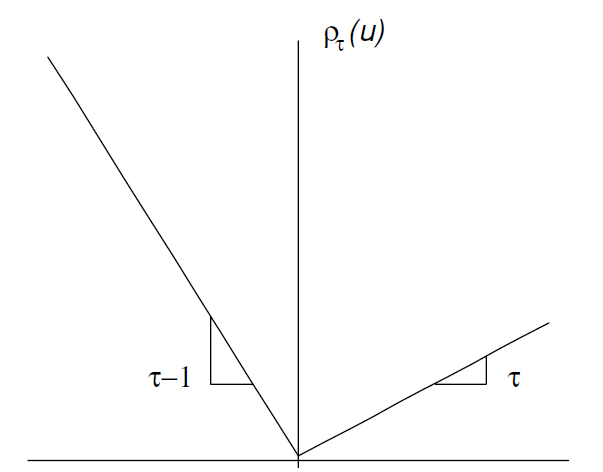
\includegraphics[width = 0.5 \textwidth]{Imagenes/perdida.png}
        \caption{Función de pérdida.}
        \label{fig:perdida}
    \end{figure}
    
    El $\tau$-ésimo cuantil se puede calcular al minimizar la función de pérdida evaluada en $X-u$ con respecto a $u$ como se muestra a continuación \cite{Koenker2005}
    
    \begin{equation}\label{minCun}
        Q_X(\tau)=\underset{u}{\arg \min } E\left(\rho_\tau(X-u)\right)=\underset{u}{\arg \min }\left\{(\tau-1) \int_{-\infty}^u(y-u) d F(x)+\tau \int_u^{\infty}(x-u) d F(x)\right\} .
    \end{equation}

    Esto se puede ver si se calcula la derivada de la ecuación \eqref{minCun} con respecto a $u$ y se igual a $0$

    \begin{equation}\label{perdidaF}
        0=(1-\tau) \int_{-\infty}^{u} d F(x)-\tau \int_{u}^{\infty} d F(x)=F(u)-\tau.
    \end{equation}

    Para el caso empírico la fórmula queda de la siguiente manera, 

    \begin{equation}\label{qestima}
        \widehat{Q}_{X}(\tau)=\arg \min _{u_\tau \in \Re}\left\{\sum_{X_i \geq u_\tau} \tau \left(X_i-u_\tau\right)+\sum_{X_i< u_\tau}(1-\tau) \left(u_\tau-X_i\right)\right\}.
    \end{equation}

    Así para un conjunto de covariables $X$, es posible ajustar una regresión $\widehat{Q}$ parra el $\tau$-ésimo cuantil de una variable respuesta usando la función de pérdida \eqref{qestima}.

    Existe varios métodos más generales de estimación de modelos de funciones cuantiles condicionales como mínimos cuadrados. Minímos cuadrados proporciona una proporciona una forma relativamente sencilla de obtener los parámetros. Para el caso donde $T = 0.5$ y los distribución de los errores son normales, se tiene la regresión lineal clásica \cite{Koenker2005}. En la Figura \ref{fig:regQ}\footnote{Figura tomada de \cite{ImgRegCuantile}}, se muestra un ejemplo de este ajuste a diferentes niveles de percentiles.

    \begin{figure}[H]
    \centering
    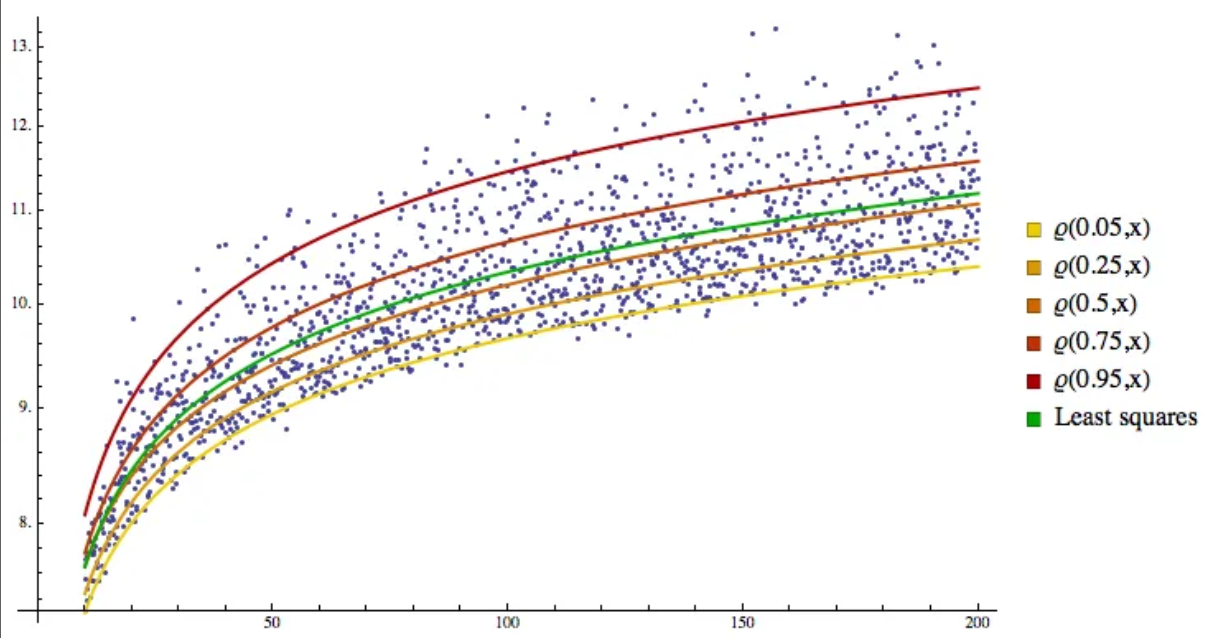
\includegraphics[width = 0.9 \textwidth]{Imagenes/Quantilsregression.png}
    \caption{Ejemplo del ajuste empleando la regresión cuantil a diferentes niveles de percentiles.}
    \label{fig:regQ}
    \end{figure}
    
%%%%%%%%%%%%%%%%%%%%%%%%%%%%%%%%%%%%%%%%%%%%%%%%%%%%%
%%%%%%%%%% Ejemplo con regresión lineal %%%%%%%%%%%%%
%%%%%%%%%%%%%%%%%%%%%%%%%%%%%%%%%%%%%%%%%%%%%%%%%%%%%

\begin{obs}[Regresión Cuantil Lineal]
    Como se hace en la clásica regresión lineal, se define $Y_i=\beta_{0, \tau}+\beta_{1, \tau} \cdot X_i+\varepsilon_{i, \tau} \quad \forall i \in\{1, \dots n\}$ con $0 < \tau < 1$, donde $\tau$ corresponde al $\tau$-ésimo cuantil de error con respecto a la variable respuesta, es decir, $Q(\varepsilon_{i, \tau}) = 0$. Entonces, usando la fórmula \eqref{qestima} se obtiene la siguiente ecuación

    \begin{equation}
        \hat{\beta}_\tau=\arg \min _{\beta_\tau \in \mathbf{R}^2}\left\{\sum_{Y_i \geq A} \tau \left|Y_i-\beta_{0, \tau}-\beta_{1, \tau} X_i\right|+\sum_{Y_i<A}(1-\tau) \left|Y_i-\beta_{0, \tau}-\beta_{1, \tau}  X_i\right|\right\}
    \end{equation}

    donde $\beta_\tau = (\beta_{0, \tau}, \beta_{1, \tau} )$ y A = $\beta_{0, \tau} + \beta_{1, \tau}X_i $. Por lo que, resolver la estimación de parámetros se convierte en un problema de programación lineal \cite{RegLinealCuantil}.
\end{obs}

%%%%%%%%%%%%%%%%%%%%%%%%%%%%%%%%%%%%%%%%%%%%%%%%%%%%%%%%%%%%%
%%%%%%%%%%  D A T O S  F U N C I O N A L E S  %%%%%%%%%%%%%%%
%%%%%%%%%%%%%%%%%%%%%%%%%%%%%%%%%%%%%%%%%%%%%%%%%%%%%%%%%%%%%

\section{Datos Funcionales}

Los datos funcionales son una forma de representar información que varía de manera continua en una dimensión o más dimensiones, como el tiempo, el espacio u otras variables continuas. En muchos experimentos estadísticos, las observaciones son funciones por naturaleza, como curvas temporales o superficies espaciales, donde la unidad básica de información es la observación funcional. Esto contrasta con los datos tradicionales, que suelen consistir en observaciones puntuales o discretas.

Un ejemplo ilustrativo de las ventajas de usar datos funcionales, tomado de \cite[Pág. 6]{Ramsay2009}, se encuentra en un estudio realizado en el hospital de San Diego. Este estudio se centró en medir el ángulo formado entre la cadera y la rodilla durante el ciclo de caminada. A diferencia de otros enfoques que se basaban en datos discretos, este estudio empleó datos funcionales para modelar la continuidad del movimiento, proporcionando una representación más detallada y precisa del ángulo a lo largo del ciclo completo. En la Figura \ref{ejemplo1}\footnote{Figura tomada de \cite{Ramsay2009}} se ilustra los datos funcionales. El intervalo $[0,1]$ representa un ciclo único y las curvas punteadas muestran la extensión periódica de los datos más allá de cualquiera de los extremos del ciclo. La ventaja de modelarlo como un continuo radica en la capacidad de capturar con mayor precisión las variaciones sutiles y los patrones dinámicos del ángulo a lo largo del ciclo completo, considerando los estados anteriores y proporcionando una representación más detallada y realista del movimiento.

\begin{figure}[H]
 \centering
  \subfloat[Ángulo formado entre la cadera y la rodilla]{
   \label{ejemplo1}
    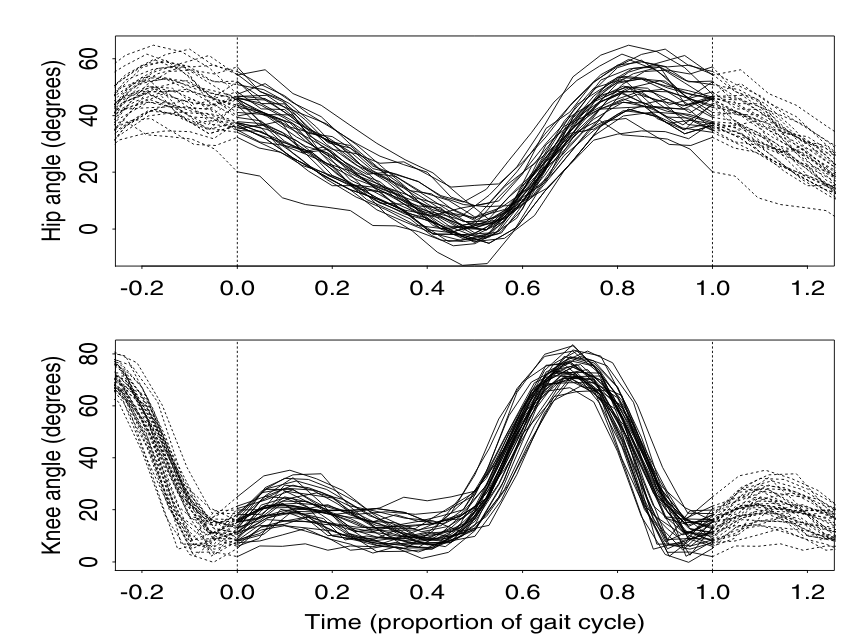
\includegraphics[width=0.45\textwidth]{Imagenes/functionalDataEj1.png}}
  \subfloat[Manuscritos]{
   \label{ejemplo2}
    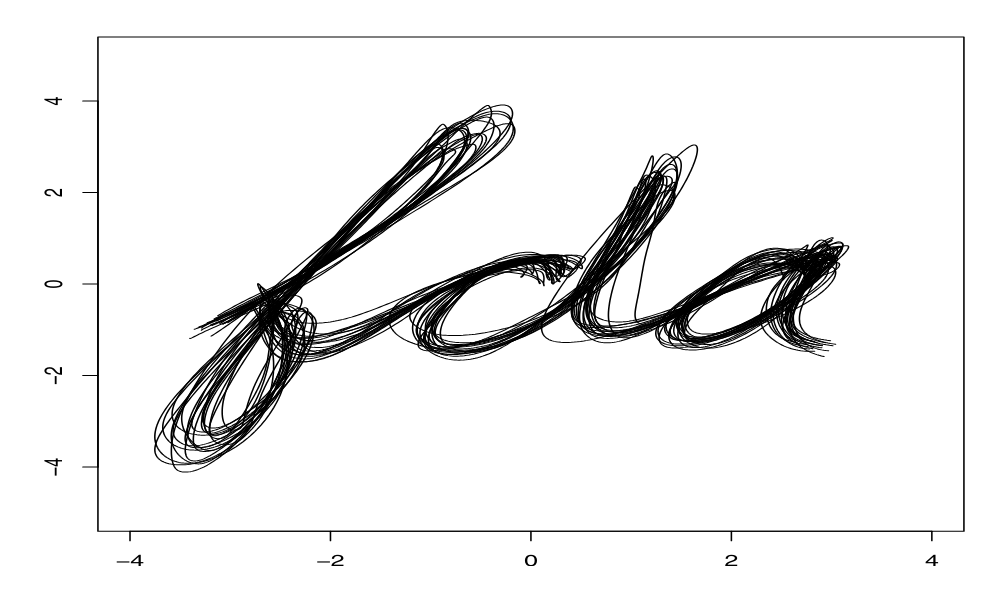
\includegraphics[width=0.45\textwidth]{Imagenes/functionalDataEj2.png}}
    \caption{Ejemplos de datos funcionales.}
    \label{fig:fdaEjemplo}
\end{figure}

Como se mencionó anteriormente, una de las utilidades de los datos funcionales es modelar el movimiento. Un caso de esta aplicación se muestra en la Figura \ref{ejemplo2} \footnote{Figura tomada de \cite{Ramsay2009}}, donde se presentan $20$ superposiciones de manuscritos. Este enfoque permite capturar las modificaciones tenues y los patrones inherentes en cada trazado, proporcionando una representación más precisa y detallada de los movimientos involucrados en la escritura \cite[Pág. 8]{Ramsay2009}.

Los datos funcionales permiten capturar la evolución de una variable a lo largo de una dimensión continua. Se emplean en una amplia gama de campos, incluyendo la estadística, la econometría, la neurociencia, la meteorología y muchas otras áreas donde es esencial modelar y comprender la evolución continua de los fenómenos \cite{boxplotFun}.

\subsection{Representación de Datos}

No siempre es posible realizar mediciones de los experimentos de interés como un continuo debido a diversos factores, como la complejidad de la medición. Por esta razón, a menudo se dispone de una serie de datos discretos que representan estas funciones. Para superar esta limitación, se utilizan técnicas de regresión y smoothing. La regresión permiten crear una función continua que ajusta los datos discretos, mientras que el smoothing ayuda a reducir el ruido y las irregularidades en los datos, proporcionando una representación más suave y precisa del movimiento.

Los datos funcionales típicamente consisten en una muestra aleatoria $x_1(t), \dots , x_n(t)$ de funciones independientes de variable real de un proceso estocástico $X(t)$ tal que $X(t) \in \mathbb{R}$,  donde $t \in \mathcal{T}$ y $\mathcal{T}$ es un intervalo en $\mathbb{R}$. Los datos funcionales se representan en enrejados discretos y finitos y comúnmente contienen errores de medición. Esto significa que, en lugar de tratar con funciones continuas en un dominio infinito, se trabaja con un conjunto finito de puntos de datos que se distribuyen a lo largo del dominio de interés. Cada punto de datos representa el valor de la función en un momento específico. Un modelo típico para las observaciones es:

\begin{equation}
     X_i(t_{il}) = \widetilde{X}_i(t_{il}) + \epsilon_{il},
\end{equation}

donde $X_i(t_{il})$ es el valor observable en $t_{il} \in \mathcal{T}$, $l = 1, \dots, L_{i}$, $i = 1, \dots, n$, $\widetilde{X}_i(t)$ es la función subyacente (suave) y $\epsilon_{il}$ son los términos de ruidos los cuales son independientes e idénticamente distribuidos \cite{Gertheiss}.

Como parte del análisis, es de interés reconstruir la función subyacente $\widetilde{X}$. Como paso inicial, se realiza un suavizamiento de la curva, tratándolo como un problema de regresión no paramétrica \cite{Gertheiss}. Entre los métodos más utilizados para este propósito se encuentran: 

\begin{itemize}
    \item Kernel Smoothing: Este método suaviza la curva utilizando un promedio ponderado de los datos cercanos, donde los pesos disminuyen con la distancia.

    \item Local Polynomial Smoothing: Similar al suavizamiento por kernel, este método ajusta un polinomio a los datos dentro de una ventana móvil. 

    \item Spline or Penalized Spline Approaches: Estos métodos utilizan funciones spline, que son piezas de polinomios ajustadas a intervalos del dominio de los datos. Los splines penalizados incluyen un término de penalización para evitar sobreajustes.
\end{itemize}

Para ejemplificar esto, se expandirá $\widetilde{X}_i = \widetilde{X}_i(\cdot)$ en una base splines. Se asume que este puede ser aproximado como una combinación lineal de splines base denotados como $\phi_{k}$, $k = 1, \dots, K$. Entonces,

\begin{equation}
     X_i(t_{il}) = \widetilde{X}_i(t_i{il}) + \epsilon_{il} = \sum_{k = 1}^{K}\phi_k(t_{il})\theta_{ik} + \epsilon_{il}
\end{equation}

con coeficientes desconocidos $\theta_{ik}$ que son estimados usando alguna técnica de optimización. 

\begin{figure}[H]
    \centering
    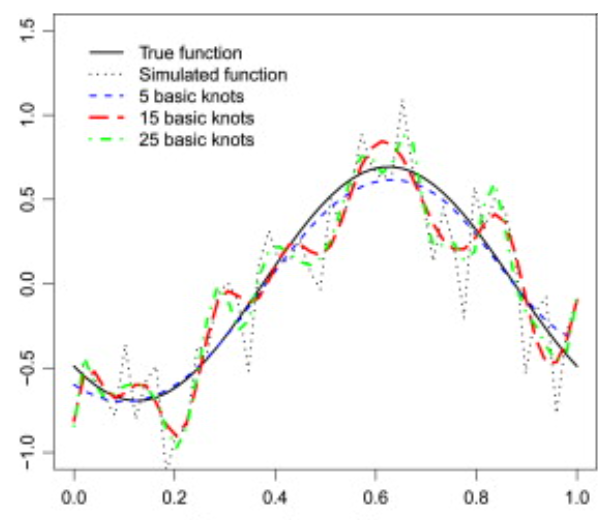
\includegraphics[width = 0.6\textwidth ]{Imagenes/splineEj.png}
    \caption{Aproximación usando splines.}
    \label{fig:ejSpline}
\end{figure}


En la Figura \ref{fig:ejSpline} \footnote{Figura tomada de \cite{Aguilera2013}}, se muestra un ejemplo de aproximación utilizando splines. Esta muestra la aproximación a la función subyacente, marcada en negro, usando datos con ruido (línea punteada) y diferentes números de splines. Un mayor número de splines produce un peor ajuste a la función subyacente, ya que no filtra el ruido de manera eficiente. Lo cual presenta un nuevo reto: determinar el número óptimo de splines para aproximar mejor la función. Por ejemplo, se ha abordado este problema utilizando splines adaptativos, validación cruzada, métodos de penalización entre otros \cite{Aguilera2013}.


Los datos funcionales continuos pueden ser complejos y difíciles de manejar debido a su naturaleza infinita. Al discretizar los datos en puntos finitos, se simplifican los cálculos y se facilitan las operaciones computacionales. Las discretizaciones permiten aplicar técnicas estadísticas y métodos de análisis de datos estándar  \cite{Aguilera2013}.

%%%%%%%%%%%%%%%%%%%%%%%%%%%%%%%%%%%%%%%%%%%%%%%%%%%%%%%%%%
\subsection{High Frequency}

En muchos campos científicos, los datos se recopilan a escalas de tiempo cada vez más finas, resultando en lo que se conoce como datos de alta frecuencia o \textit{High Frequency}. Estos datos capturan eventos y cambios con una resolución temporal muy detallada, permitiendo un análisis más granular y preciso de los fenómenos estudiados. Un ejemplo de la aplicación de este tipo de datos es en finanzas, donde la alta frecuencia permite comprender mejor las microestructuras del mercado \cite{Tsay2000}.

 En aplicaciones como el análisis de movimiento humano o la escritura a mano, los datos funcionales derivados de datos de alta frecuencia ofrecen una representación más realista y detallada, permitiendo una comprensión más profunda de los fenómenos estudiados. Los datos funcionales son especialmente aplicables con datos de alta frecuencia porque las herramientas estadísticas de FDA suelen depender de alguna forma de suavizado para transformar datos de alta dimensión o incompletos en una curva más suave. Esta curva puede ser descrita por un número menor de parámetros o un modelo parámetro, facilitando así el análisis y la interpretación de datos complejos y detallados \cite{Miao2013}.

 
%%%%%%%%%%%%%%%%%%%%%%%%%%%%%%%%%%%%%%%%%%%%%%%%%%%%%%%%%%

\subsection{Banda de Profundidad para Datos Funcionales}

Una de las grandes dificultades al realizar el análisis de datos funcionales es poder establecer comparaciones sobre la distribución de estos datos. Sin embargo, esta tarea se complica aún más cuando se trata de datos funcionales multivariados. A diferencia de los datos tradicionales, donde la escala es la principal herramienta de comparación, en el caso de los datos funcionales, lo relevante es su forma a lo largo del tiempo o de otra dimensión continua.

Por esta razón, López-Pintado y Romo introdujeron una noción de bandas de profundidad, la cual permite asignarles un orden teniendo en cuenta los aspectos anteriormente mencionados, es decir, una noción de estadísticos de orden con datos funcionales \cite{RomoPintado}. Estas bandas de profundidad proporcionan una forma de comparar y ordenar datos funcionales multivariados, lo que facilita su análisis y comprensión en estudios estadísticos y científicos. Posteriormente, Ying Sun y Marc Genton desarrollaron una metodología para crear boxplots con datos funcionales en su artículo `Functional Boxplots' \cite{boxplotFun}.

Sea $x_{[i]}(t)$ la curva muestral asociada al $i$-ésimo dato más profundo. Se denotará por $x_{[1]}(t), \dots, x_{[n]}(t)$ a los estadísticos de orden, donde $x_{[1]}(t)$ representa la curva más profunda y central, o la mediana, mientras que $x_{[n]}(t)$ representa la curva más atípica.


\begin{defn}[Banda]
    Se define la gráfica de la función $x(t)$ como un subconjunto en el plano $G(x) =  \left\{ (t, x(t)): t \in \mathcal{I} \right\}$. Se define la banda delimitada por las curvas $x_1, \dots, x_n$ como,
    
    \begin{equation}
        B\left(x_{i_1}, \ldots, x_{i_k}\right)=\left\{(t, u(t)): t \in \mathcal{I}, \min_{r=1, \ldots, k} x_{i_r}(t) \leq u(t) \leq \max _{r=1, \ldots, k} x_{i_r}(t)\right\}.
    \end{equation}
\end{defn}

\begin{defn}[Banda de Profundidad Poblacional]
    Sea $J$ el número de curvas que determinan la banda, donde $J$ es número fijo entre $2 \leq J \leq n$. Para copias $x_1(t), \dots, x_n(t)$ independientes de un proceso $X(t)$, la banda de profundidad poblacional definida para una curva $x(t)$ con respecto a la medida de probabilidad $P$, se define como:

    \begin{equation}
        \mathrm{BD}_J(x, P)=\sum_{j=2}^J \mathrm{BD}^{(j)}(x, P)=\sum_{j=2}^J P\left\{G(x) \subset B\left(X_1, \ldots, X_j\right)\right\},
    \end{equation}

    donde $B(X_1, \dots, X_j)$ es la banda delimitada por $j$ curvas aleatorias.
\end{defn}

La versión muestral de la $\mathrm{BD}^{j}(x, P)$ es obtenida calculando la fracción de bandas determinadas por $j$ diferentes observaciones que contienen la gráfica de $x(t)$

\begin{equation}
    \mathrm{BD}_n^{(j)}(x)= \binom{n}{j}^{-1} \sum_{1 \leq i_1<i_2<\cdots<i_j \leq n} \mathbbm{1}\left\{G(x) \subseteq B\left(x_{i_1}, \ldots, x_{i_j}\right)\right\}.
\end{equation}

En otras palabras, se está calculando la proporción de bandas que contiene a la de gráfica $x(t)$. Esto implica que cuanto mayor sea esta fracción, más central será la posición de la curva. En términos prácticos, una fracción más grande indica que la curva es más cercana a la gráfica `central'.

Así, la profundidad muestral de banda de la gráfica $x(t)$ está determinada por

\begin{equation}
    \mathrm{BD}_{n, J(x)} = \sum_{j = 2}^{J} \mathrm{BD}_n^{(j)}(x).
\end{equation}

Para comprender mejor cómo calcular la profundidad de banda, a continuación se presenta un ejemplo sencillo que involucra cuatro observaciones, el cuál es tomado de \textit{Functional Boxplots} \cite{boxplotFun}.

\begin{ejemplo}
   En la Figura \ref{fig:CurvasX}\footnote{
Figura tomada de \cite{boxplotFun}}, se muestra un escenario con 4 observaciones. Para calcular la profundidad de cada observación, es necesario construir las bandas considerando grupos de $2, 3$ y $4$ observaciones.
    
    Para $J = 2$ hay $6$ posibles bandas, es decir las combinaciones de $4$ en $2$, las cuales son $B(x_1, x_2)$, $B(x_1, x_3)$, $B(x_1, x_4)$, $B(x_2, x_3)$, $B(x_2, x_4)$ y $B(x_3, x_4)$. En la Figura \ref{fig:CurvasX}, se muestra en gris la banda entre $x_1$ y $x_3$, y se puede apreciar que las curvas que contiene esta banda son $x_1, x_2$ y $x_3$. En la Ecuación \eqref{j2}, se muestran todas las bandas con las curvas que contienen cada una.
    
    \begin{equation}\label{j2}
        \begin{matrix}
        x_1,x_2 \subseteq  B(x_1, x_2),  & x_2,x_3 \subseteq  B(x_2, x_3), \\
        x_1,x_2, x_3 \subseteq  B(x_1, x_3),  & x_2,x_4 \subseteq  B(x_2, x_4), \\
        x_1,x_2, x_4 \subseteq  B(x_1, x_4),  & x_3,x_4 \subseteq  B(x_3, x_4), \\
    \end{matrix}
    \end{equation}

    Por lo tanto, la profundidad de banda muestral para $j = 2$ de cada observación es la siguiente:

    \begin{equation}
        \begin{matrix}
            \mathrm{BD}^{2}_4(x_1) = \frac{3}{6}, & \mathrm{BD}^{2}_4(x_2) = \frac{5}{6},  & \mathrm{BD}^{2}_4(x_3) = \frac{3}{6},  & \mathrm{BD}^{2}_4(x_4) = \frac{3}{6}. \\
        \end{matrix}        
    \end{equation}
    
    \begin{figure}[H]
    \centering
    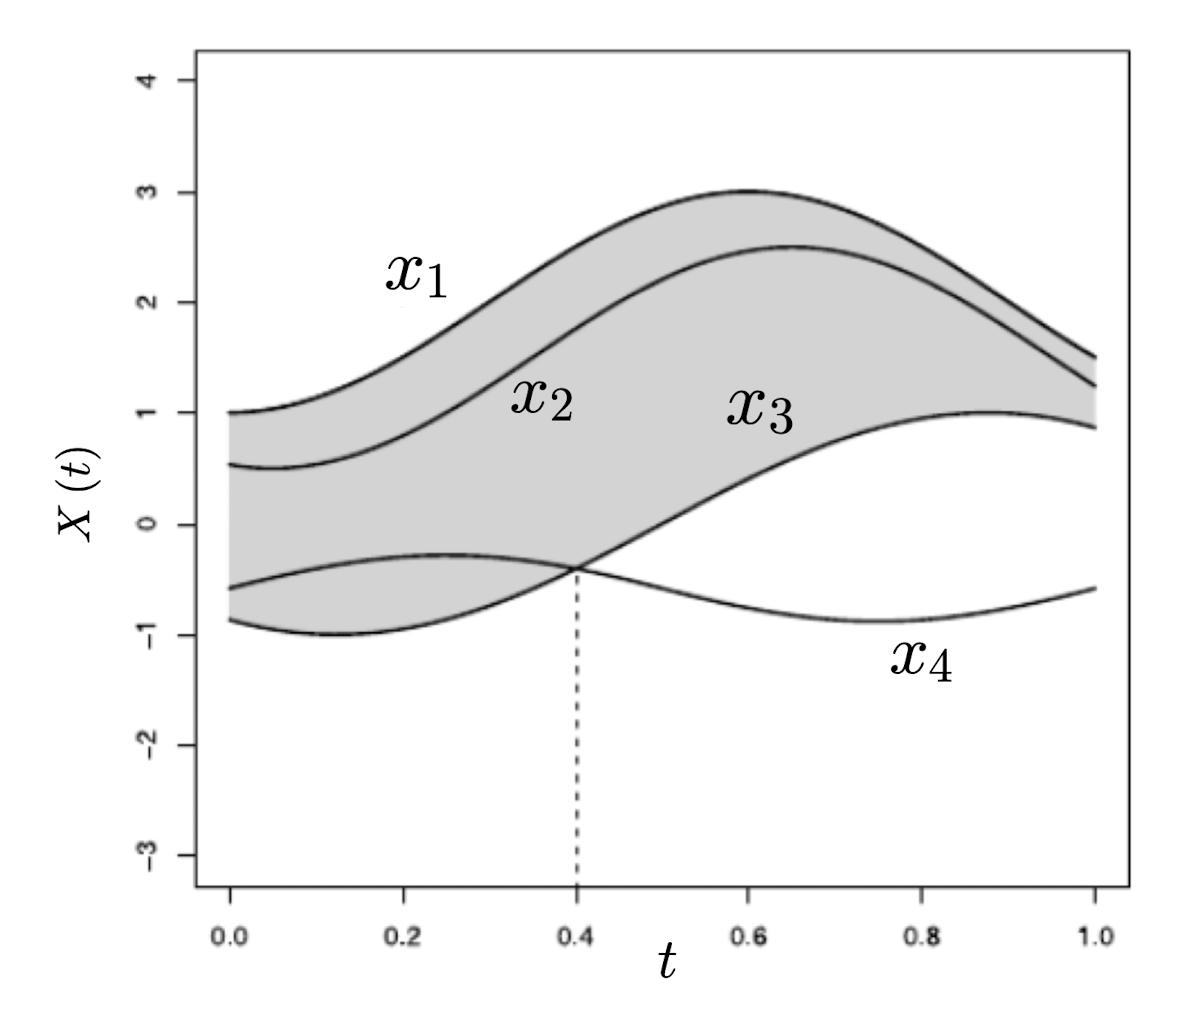
\includegraphics[width = 0.6 \textwidth]{Imagenes/WhatsApp Image 2024-04-21 at 8.06.25 PM.jpeg}
    \caption{Ejemplo de gráfico para la medida de profundidad.}
    \label{fig:CurvasX}
\end{figure}

Ahora, hay que repetir el proceso para $J = 3$. En la Ecuación \eqref{j3} se muestran las bandas y sus respectivas observaciones que están contenidas. En la Ecuación \eqref{BDJ3} se muestra el nivel de profundidad de cada observación.

\begin{equation}\label{j3}
    \begin{matrix}
        x_1, x_2, x_3 \subseteq B(x_1, x_2, x_3), & x_1, x_2 x_3, x_4 \subseteq B(x_1, x_3, x_4), \\
        x_1, x_2, x_4 \subseteq B(x_1, x_2, x_4), & x_2, x_3, x_4 \subseteq B(x_2, x_3, x_4), \\
    \end{matrix}
\end{equation}

\begin{equation}\label{BDJ3}
    \begin{matrix}
        \mathrm{BD}^{3}_4(x_1) = \frac{3}{4}, & \mathrm{BD}^{3}_4(x_2) = \frac{4}{4},  & \mathrm{BD}^{3}_4(x_3) = \frac{3}{4},  & \mathrm{BD}^{3}_4(x_4) = \frac{3}{4} \\
    \end{matrix} 
\end{equation}

Finalmente, para $J = 4$, se tiene que la única banda es $B(x_1, x_2, x_3, x_4)$ que contiene a todas las curvas. Por lo tanto, el valor de profundidad de cada variable es:

\begin{equation}
    \begin{matrix}
            \mathrm{BD}^{2}_4(x_1) = 1, & \mathrm{BD}^{2}_4 (x_2) = 1,  & \mathrm{BD}^{2}_4(x_3) = 1,  & \mathrm{BD}^{2}_4(x_4) = 1. \\
        \end{matrix}    
\end{equation}

Para calcular el nivel total de profundidad, simplemente se necesita sumar las profundidades de cada variable para todos los valores de $J$

\begin{equation}
    \begin{matrix}
\mathrm{BD}_{n, J}(x_1) = \frac{3}{6} + \frac{3}{4} + 1 = \frac{9}{4} = 2.25, \\
\mathrm{BD}_{n, J}(x_2) = \frac{5}{6} + \frac{4}{4} + 1 = \frac{9}{4} = 2.83, \\
\mathrm{BD}_{n, J}(x_3) = \frac{3}{6} + \frac{3}{4} + 1 = \frac{9}{4} = 2.25, \\
\mathrm{BD}_{n, J}(x_4) = \frac{3}{6} + \frac{3}{4} + 1 = \frac{9}{4} = 2.25.
\end{matrix}
\end{equation}

Así, resulta que $x_2$ es la banda más profunda.

\end{ejemplo}

%%%%%%%%%%%%%%%%%%%%%%%%%%%%%%%%%%%%%%%%%%%%%%%%%%%%%%%
\subsubsection{Banda de Profundidad Modificada}

Además, López Pintado y Romo propusieron una definición más flexible: la banda de profundidad modificada. Esta metodología se encarga de medir la proporción de tiempo que la curva $x(t)$ pasa dentro de la banda \cite{boxplotFun}

\begin{equation}
    \operatorname{MBD}_n^{(j)}(x) = \binom{n}{j}^{-1} \sum_{1 \leq i_1<i_2<\cdots<i_j \leq n} \lambda_r \left\{ A(x ; x_{i_{1}}, \dots, x_{i_{j}}\right\} \text{ donde, }
\end{equation}

\begin{equation}
     A_j(y) \equiv A\left(y ; y_{i_1}, \ldots, y_{i_j}\right) \equiv \left\{t \in \mathcal{I}: \min _{r=i_1, \ldots, i_j} y_r(t) \leq y(t) \leq \max _{r=i_1, \ldots, i_j} y_r(t) \right\},
\end{equation}

\begin{equation}
    \lambda_r(x) = \lambda(A_j(x))/\lambda(\mathcal{I})
\end{equation}

y $\lambda$ es la medida de Lebesgue en $\mathcal{I}$.
%%%%%%%%%%%%%%%%%%%%%%%%%%%%%%%%%%%%%%%%%%%%%%%%%%%%%%%%%%
%%%%%%%% M E J O R A C I O N  D E  L A  T B D %%%%%%%%%%%%
%%%%%%%%%%%%%%%%%%%%%%%%%%%%%%%%%%%%%%%%%%%%%%%%%%%%%%%%%%
\subsubsection{Transformación de Translación con Signo de Profundidad}

    Para mejorar la interpretación, en el trabajo doctoral de Israel Emmanuel Ambriz Lobato, bajo la dirección de la Dra. Graciela González y el Dr. Emilien Joly, se propone una nueva metodología para calcular el orden de los datos funcionales, la cual es llamada \textit{Signed Translation transformed Depth} (STtD). Esta innovación introduce la noción de la banda de profundidad transformada como se muestra en la Ecuación \eqref{TBD} \cite{BandaEmanuel}.
    
    \begin{defn}
        Sea  $x_1(t), \dots , x_n(t)$ un conjunto de muestras funcionales independientes del proceso estocástico $X(t)$ real-valuado,  donde $t \in \mathcal{T}$ y $\mathcal{T}$ es un intervalo en $\mathbb{R}$. La \textit{Signed Translation transformed Depth} está dada por:

    \begin{equation}\label{TBD}
    STtD(x)=\left(T B D^*(x)-T B D^*\left(x_{[1]}\right)\right) \operatorname{sign}\left(\int_{\mathcal{I}}\left(x(t)-x_{[1]}(t)\right) d t\right),
    \end{equation}

    donde
    \begin{equation}\label{posicion}
        T B D^*(x)=(1-B D(x)).
    \end{equation}

    La ecuación \eqref{posicion} se encarga de posicionar las curvas más profundas cerca del $0$ y las más lejanas cerca del $1$. La ecuación \eqref{TBD} se encarga de asignarles un signo.
        
    \end{defn}


La banda de profundidad transformada redefine la forma en que se calcula el orden de los datos funcionales. A continuación, se destacan algunos aspectos importantes de esta nueva metodología para su futura interpretación e implementación:

\begin{enumerate}
    \item $STtD(x(t)) \in (-1, 1), \text{ para todo } x(t)$,
    \item $STtD(x_{[1]}(t)) = 0,$
    \item Si $STtD(x(t)) > 0$ significa que la curva pasa más tiempo por arriba de $x_{[1]}(t)$,
    \item Si $STtD(x(t)) < 0$ significa que la curva pasa más tiempo por abajo de $x_{[1]}(t)$.
\end{enumerate}

Para ilustrar cómo esta transformación afecta, en la Figura \ref{fig:ComparaBandas} \footnote{Figura tomada de \cite{BandaEmanuel}}, se presentan dos histogramas obtenidos a partir de un conjunto de datos analizados en el trabajo doctoral de Emmanuel Ambriz. En el histograma izquierdo se muestran las medidas de profundidad para dicho conjunto de datos, el cual no es interpretable en términos de la ubicación de los datos atípicos con respecto a la mediana.

\begin{figure}[H]
    \centering
    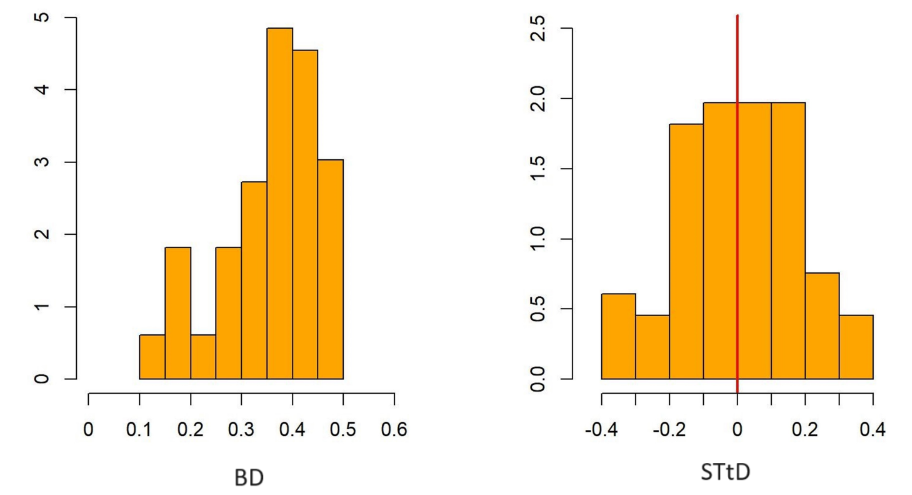
\includegraphics[width = 0.7 \textwidth]{Imagenes/comparacionBandas.png}
    \caption{Comparación visual de la medida banda de profundidad y la medida transformación de translación con signo de profundidad.}
    \label{fig:ComparaBandas}
\end{figure}

En contraste, en el histograma derecho se presentan las medidas utilizando la profundidad de banda transformada. Debido a la forma en que fue construida, se puede observar cierta simetría; además, se pueden identificar fácilmente los valores atípicos tanto por encima como por debajo de la curva.

%%%%%%%%%%%%%%%%%%%%%%%%%%%%%%%%%%%%%%%%%%%%%%%%%%%%%%%%%%
%%%%%%%% M E J O R A C I O N  D E  L A  T B D %%%%%%%%%%%%
%%%%%%%%%%%%%%%%%%%%%%%%%%%%%%%%%%%%%%%%%%%%%%%%%%%%%%%%%%

\section{Transformación de Variables Funcionales}

Como se detallará más exhaustivamente en el Capítulo \ref{Resultados}, una parte de la base de datos que se empleará para crear el modelo, consiste en mediciones de glucosa e insulina tomadas durante la prueba de tolerancia a la glucosa oral en los minutos $0$, $30$, $60$, $90$ y $120$. Estas observaciones se pueden considerar como curvas y, por lo tanto, constituyen los datos funcionales con los que se hará inferencia para proporcionar la probabilidad de padecer diabetes. 

Llámese $g(t)$ y $\eta(t)$ a las variables funcionales que representan los niveles de glucosa e insulina, respectivamente, donde $t = 0, 30, 60, 90, 120$. En la Figura \ref{fig:pairsTBD}, se muestran gráficos de dispersión, en los que el eje $x$ representa la profundidad de banda transformada con signo de la variable funcional glucosa, mientras que en el eje $y$ se muestra la profundidad de la variable funcional de insulina. Asi, cada punto representa la $STtD$ asociadas las curvas de glucosa e insulina de un individuo en la muestra. Según ciertos criterios determinados por mediciones de la OGTT (los cuales se detallarán en el Capítulo \ref{Resultados}), es posible realizar un prediagnóstico de los individuos clasificados como normales, prediabéticos y diabéticos. Estas categorías están coloreadas en los gráficos de dispersión, junto con la distribución de las bandas de profundidad transformada con signo en insulina y glucosa.

Un aspecto importante a destacar, en la Figura \ref{fig:pairsTBD}, es que la transformación de la banda de profundidad con signo de la variable glucosa muestra una distribución característica para cada categoría del prediagnóstico. En cuanto a la variable correspondiente a la insulina, no parece haber una separación clara entre las categorías. Sin embargo, en los gráficos de dispersión se puede observar con mayor claridad el comportamiento que se busca analizar.

\begin{figure}[H]
    \centering
    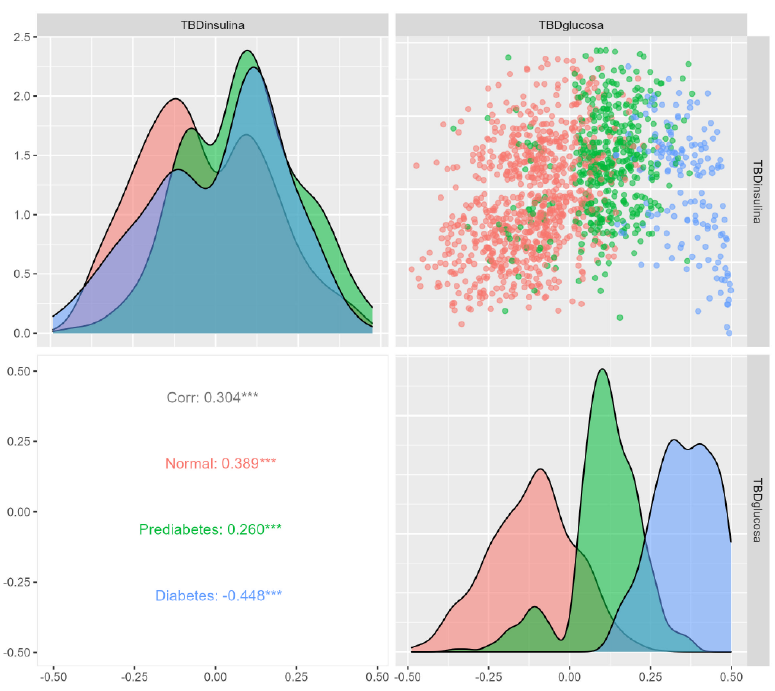
\includegraphics[width = 0.7 \textwidth]{Imagenes/pairsTBDS.png}
    \caption{Histogramas y gráficos de dispersión para las STtD's de las variables glucosa e insulina.}
    \label{fig:pairsTBD}
\end{figure}


Los altos niveles de glucosa se corresponden con bajos niveles de insulina, ya que la producción de insulina disminuye; lo cual se respalda con el signo negativo de la correlación en la categoría diabética. Esto es un poco complicado de ver en la Figura \ref{fig:pairsTBD} pero la correlación aclara esto. Por otro lado, los bajos niveles de glucosa también se asocian con bajos o medianos niveles de insulina, lo que indica un funcionamiento adecuado de la insulina en la categoría normal, donde el signo de la correlación es positivo.

En cuanto a los individuos prediabéticos se observa que presentan niveles altos tanto de glucosa como de insulina. Aunque la correlación es positiva, es importante notar que los valores de insulina alcanzan un máximo y luego descienden, lo que indica una posible falla irreversible de las células beta.

Además, en el punto $(0, 0)$, que corresponde a las medianas de cada variable, se puede observar una división por cuadrantes. Esto sugiere que, según esta división, se pueden clasificar a los individuos, y este será un punto de partida esencial para el presente trabajo. Sin embargo, es importante tener en cuenta que este punto puede ser modificado según criterios médicos, ya que podría ser preferible ajustarlo para disminuir la probabilidad de cometer errores de tipo $2$.

%%%%%%%%%%%%%%%%%%%%%%%%%%%%%%%%%%%%%%%%%%%%%%%%%%%%%%%%%
\subsection{Creación de Variable Respuesta}

Defínase el punto $\widetilde{TBD} = (\widetilde{TBD^g}, \widetilde{TBD^{\eta}})$ que representa los valores límite aceptables de glucosa e insulina para pacientes completamente sanos. A partir del punto $(\widetilde{TBD^g},\widetilde{TBD^{\eta}})$ se define la función cuadrante para cada observación como:

\begin{equation}
     C_ i = \left\{\begin{matrix}
1, & TBD_{i}^{g} < \widetilde{TBD^{g}}, TBD_{i}^{\eta} < \widetilde{TBD^{\eta}}\\
2, & TBD_{i}^{g} < \widetilde{TBD^{g}}, TBD_{i}^{\eta} > \widetilde{TBD^{\eta}}\\
3, & TBD_{i}^{g} > \widetilde{TBD^{g}}, TBD_{i}^{\eta} < \widetilde{TBD^{\eta}}\\
4, & TBD_{i}^{g} > \widetilde{TBD^{g}}, TBD_{i}^{\eta} > \widetilde{TBD^{\eta}}
\end{matrix}\right.
\end{equation}

\begin{enumerate}
    \item El primer cuadrante, denotado como $C_i = 1$, corresponde al cuadrante inferior izquierdo y se asocia con los pacientes \textbf{completamente sanos}. Estos pacientes presentan niveles estables tanto de glucosa como de insulina.
    \item El segundo cuadrante, asociado con $C_i = 2$, comprende a los pacientes que presentan \textbf{resistencia a la insulina o predisfunción de las células beta}. Estos pacientes han comenzado a aumentar sus niveles de insulina para mantener estable su glucosa. Quienes están en este cuadrante tienen una alta probabilidad de regresar al cuadrante $1$ mediante la mejora de hábitos dietéticos y de ejercicio físico.
    \item El tercer cuadrante, relacionado con $C_i = 3$, se refiere a los pacientes con \textbf{resistencia a la insulina o estrés en las células beta}. Estos pacientes, a pesar de experimentar un aumento en sus niveles de insulina, no logran mantener estables sus niveles de glucosa; lo cual indica una disminución en su sensibilidad a la insulina. Tienen una probabilidad muy baja de regresar a los cuadrantes 1 o 2 mediante la mejora de hábitos dietéticos y de ejercicio, lo que sugiere que es probable que hayan desarrollado resistencia a la insulina.
    \item En el cuarto cuadrante, identificado como $C_i = 4$, se encuentran los pacientes con \textbf{resistencia a la insulina y disfunción evidente de las células beta}. Estos pacientes requieren la administración de insulina para mantener estables sus niveles de glucosa, y tienen escasas posibilidades de regresar a alguno de los cuadrantes previos.
\end{enumerate}

Usando los cuadrantes se define la siguiente función

\begin{equation}
    m_i= \begin{cases}
    \widehat{F}^g\left(T B D_i^g\right) \cdot \widehat{F}^\eta\left(T B D_i^\eta\right), & C_i=1, \\ \widehat{F}^g\left(T B D_i^g\right) \cdot\left(1-\widehat{F}^\eta\left(T B D_i^\eta\right)\right), & C_i=2, \\ \left(1-\widehat{F}^g\left(T B D_i^g\right)\right) \cdot\left(1-\widehat{F}^\eta\left(T B D_i^\eta\right)\right), & C_i=3, \\ \left(1-\widehat{F}^g\left(T B D_i^g\right)\right) \cdot \widehat{F}^\eta\left(T B D_i^\eta\right), & C_i=4,\end{cases}
\end{equation}


donde $\widehat{F}^g$ y $\widehat{F}^{\eta}$ representan la función empírica de los valores de \textit{Signed Translation transformed Depth} de los datos funcionales correspondientes a la glucosa y la insulina, respectivamente. Esta función desempeña el papel de funciones de ponderación. Posteriormente se procede a computar la siguiente función:

\begin{equation}
    F B I / G C_i= \begin{cases}\left(M_1-m_i\right) / M_1, & C_i=1, \\ \left(m_i-M_2\right) / M_2, & C_i=2, \\ \left(m_i-M_3\right) / M_3-1, & C_i=3, \\ \left(m_i-M_4\right) / M_4-2, & C_i=4,\end{cases}
\end{equation}

donde $M_k =  \displaystyle \max_{m_i \in C_k} m_i$ para $k = 1, 2, 3, 4$ y $FBI/GC$ son las siglas de \textit{Functional Based Insulin/Glucose Classification}.


Con el fin de establecer un cierto orden en la condición de las células beta, se realiza un escalado utilizando el máximo de cada cuadrante y restando una constante. Este procedimiento permite estandarizar los valores y facilitar la comparación entre diferentes grupos de pacientes proporcionando una medida relativa de la función de las células beta en relación con el estado de salud.

\begin{enumerate}
    \item En el cuadrante $1$, asociado con pacientes \textbf{completamente sanos}, la variable respuesta se encuentra en el rango $0 \leq \text{FBI/GC} \leq 1$.
    \item En el cuadrante $2$, correspondiente a los pacientes con \textbf{resistencia a la insulina o predisfunción de la célula beta}, la variable creada anteriormente se encuentra en el rango $-1 \leq \text{FBI/GC} \leq 0$.
    \item En el cuadrante $3$, que comprende a los pacientes con \textbf{resistencia a la insulina y estrés en la célula beta}, se tiene que $-2 \leq \text{FBI/GC} \leq -1$.
    \item En el cuadrante 4 se encuentran los pacientes con \textbf{resistencia a la insulina y disfunción evidente de la célula beta}, donde $-3 \leq \text{FBI/GC} \leq -2$.
\end{enumerate}

 Luego de llevar a cabo todos los cálculos mencionados anteriormente, se ha logrado construir una variable numérica que encapsula toda la información esencial extraída de los datos funcionales obtenidos de las curvas de glucosa e insulina. Esta variable condensa de manera efectiva la complejidad de los datos originales en una forma que resulta conveniente para el ajuste del modelo de regresión cuantil.
\cleardoublepage

%%%%%%%%%%%%%%%%%%%%%%%%%%%%%%%%%%%%%%%%%%%%%%%%%%%%%%%%%%%%
%%%%%%%%%%%          C O P U L A S         %%%%%%%%%%%%%%%%%
%%%%%%%%%%%%%%%%%%%%%%%%%%%%%%%%%%%%%%%%%%%%%%%%%%%%%%%%%%%%

\chapter{Cópulas}

En este capítulo se definirá el concepto de cópulas, que constituye la herramienta principal para modelar las dependencias entre las covariables. Se hará especial hincapié en las cópulas bivariadas, ya que, dada una función de distribución de un vector aleatorio, esta puede representarse como el producto de cópulas bivariadas condicionales. Esta forma de descomposición se conoce como R-Vines. Sin embargo, esta descomposición no es única, ya que diferentes representaciones pueden obtenerse al permutar el orden de descomposición. En particular, se detallará una forma llamada D-Vine, que se asocia con un grafo o árboles. Utilizando el grafo, es sencillo visualizar las dependencias condicionales o cópulas condicionales necesarias para realizar regresiones utilizando las estructuras mencionadas.

Uno de los principales resultados en los que se basa la teoría de cópulas es el Teorema de Sklar \ref{TeoSklar}. Este teorema proporciona la noción fundamental de las cópulas al establecer una relación entre la función de distribución conjunta de cualquier vector de variables aleatorias y sus distribuciones marginales, que no necesariamente deben ser conocidas. 


\begin{teor}[Teorema de Sklar]\label{TeoSklar}
    \begin{enumerate}
    \item Para cada función de distribución $H$ con distribuciones marginales univariadas $F_1, \dots, F_d$, existe una cópula $C$ $d-dimensional$ tal que 
    \begin{equation}\label{eqsklar}
        H(x) = C(F_1(x_1), F_2(x_2), \dots, F_d(x_d)), \quad x \in \mathbb{R}^{d},
    \end{equation}

    La cópulas C esta únicamente definida en $\prod_{j = 1}^{d}ran F_j$ y esta definida por

    \begin{equation}
        C(u) = H(F_1^{\leftarrow}(u_1), \dots, F_d^{\leftarrow}(u_d)), \quad u \in \prod_{j = 1}^{d}ran F_j
    \end{equation}
    %%%%%%%%%%%%%%%%%%%%%%%%%%%%%%%%%%%%
    
    \item Por el contrario, dada una cópula $C$ $d-dimensional$ y funciones de distribución univariadas $F_1, \dots, F_d$ y$H$ definida como en \eqref{eqsklar}, es una función de distribución $d$ $dimensional$ con marginales $F_1, \dots, F_d$. \cite{CopulasR}
    \end{enumerate}
\end{teor}

El teorema de Sklar establece que cualquier función de distribución conjunta puede descomponerse en sus distribuciones marginales y una cópula. Esto es posible gracias al resultado de la transformación integral de probabilidad \eqref{PITdist}, que indica que cualquier distribución continua puede transformarse en una distribución uniforme estándar. Por lo tanto, una cópula descompone esta distribución conjunta, cuyas marginales pueden ser complejas, en términos de otra función de distribución cuya característica es que sus distribuciones marginales son uniformes en el intervalo $[0,1]$. Esta descomposición permite estudiar la dependencia entre las variables de manera independiente de las distribuciones marginales originales.

Como resumen, dado un vector $X = (X_1, \dots, X_d)$ con funciones de distribución marginal $F_1, \dots, F_d$, existe una cópula $C$ asociada a $X$. Si solo se está interesado en la estructura de dependencia de $X$, se puede considerar la escala $u$ o la escala cópula aplicando la transformación integral de probabilidad a sus marginales $U_j := F_j(X_j), j = 1, \dots, d$.

En conclusión, es importante destacar que las distribuciones marginales de la cópula no contienen información sobre cómo cada variable aleatoria puede interactuar con las demás. Toda la información sobre su dependencia se encuentra en la función de cópula subyacente.

\section{Conceptos Preliminares}

Una copula en palabras generales, es una distribución multivariada con funciones de densidad marginales uniforme estándar, esta es la conexión de las marginales con la distribución conjunta de ahí el nombre de copula. Estas son utilizadas para modelar la dependencia entre múltiples variables las cuales no son necesariamente lineales lo cual permite capturar patrones de correlación no lineal y asimétrica, lo que puede ser útil en la detección de anomalías, la segmentación de datos. Estas pueden ser paramétricas como no paramétricas \cite{CopulasR}.

Además, las cópulas se modelan a través de los datos, lo que permite capturar y modelar de manera precisa las relaciones de dependencia entre las variables. Esto proporciona una herramienta poderosa para analizar y entender las interacciones complejas en conjuntos de datos multivariados.


\begin{defn}[Subcópula]
    Una subcópula 2-dimensional es una función $C'$ con las siguientes propiedades:

    \begin{enumerate}
        \item \textbf{Dominio}: El dominio de la subcópula $C'$ es el producto cartesiano de dos subconjuntos $S_1$ y $S_2$ del intervalo $[0, 1]$, denotado como $S_1 \times S_2$.

        \item \textbf{Aterrizado (Grounded) y 2-creciente}: Grounded quiere decir que, $C(0,v)=0$ y $C(u,0)=0$ para todo $u$ en $u \in S_1$ y $v \in S_2$. 
        $2$-creciente, significa que para cualquier valor fijo de un argumento, aumentar el otro argumento nunca disminuye el valor de $C$.

        \item \textbf{Condición sobre los márgenes}: Para cada $u$ en $S_1$ y $v$ en $S_2$, 
        \begin{equation}
            C'(u, 1) = u, \quad C'(1, v) = v
        \end{equation}

        es decir, cuando se fija uno de los argumentos, la subcópula se comporta como la respectiva distribución marginal
    \end{enumerate}
\end{defn}


\begin{defn}[Cópula 2 dimensional]
    Una cópula bidimensional (o 2-cópula, o simplemente, una cópula) es una 2-subcópula $C$ cuyo dominio es el conjunto $I^2$. Donde $I$ es el intervalo unitario $[0,1]$. 
\end{defn}



\begin{defn}[Subcópula n-dimensional]
    Una subcópula n-dimensional es una función $C'$ con las siguientes propiedades:

    \begin{enumerate}
        \item \textbf{Dominio}: El dominio de la subcópula $C'$ es el producto cartesiano de n subconjuntos $S_i $ para $ i = \left\{ 1, \dots, n\right\}$ del intervalo $[0, 1]$, denotado como $S_1 \times \cdots \times S_n$.

        \item \textbf{Aterrizado (Grounded) y n-creciente}: Grounded quiere decir que, $C(u_1, \dots, u_n)=0$ si alguna $u_i = 0$, para todo $u_1$ en $u_1 \in S_i$. 
        $n$-creciente, significa que para cualquier valor fijo de un argumento, aumentar el otro argumento nunca disminuye el valor de $C$.

        \item \textbf{Condición sobre los márgenes}: Para cada $u_i$ en $S_i$ para $i =  \left\{ 1, \dots, n\right\}$, 
        \begin{equation}
            C'(1, \dots, u_i, \dots,  1) = u_i, \quad \left\{ 1, \dots, n\right\}
        \end{equation}

        es decir, cuando se fija uno de los argumentos, la subcópula se comporta como la respectiva distribución marginal
    \end{enumerate}
\end{defn}

En otras palabras, una cópula es una subcópula bidimensional cuyo dominio abarca todo el cuadrado unitario $[0, 1]^2$. Esto significa que la cópula relaciona las distribuciones marginales de dos variables aleatorias y describe la estructura de dependencia conjunta entre ellas a lo largo de todo el rango posible de valores que pueden tomar \cite{nelsenintroduction}.

\begin{defn}[Cópula n dimensional]
    Una cópula n dimensional es una 2-subcópula $C$ cuyo dominio es el conjunto $I^n$. Donde $I$ es el intervalo unitario $[0,1]$. 
\end{defn}

\begin{ejemplo}[Cópula Producto]
    La cópula más sencilla que se construye consiste en multiplicar las funciones de distribución marginales de las variables aleatorias individuales.

    Sea $X = (X_1, X_2)$ donde cada entrada del vector aleatorio tiene como función de distribución $X_i \sim F(X_i)$, si se define $u_i = F(x_i)$ entonces,

    \begin{equation}
         \prod (u_1, u_2) = u_1 \cdot u_2
    \end{equation}

    es una cópula.

    Esto es claro, ya que cada $u_i \sim U(0, 1)$, haciendo la transformación integral de probabilidad \ref{PITdef} y es función de distribución pues es la definición de variables aleatorias independiente. Cabe mencionar que Si dos variables aleatorias $X$ e $Y$ están relacionadas a través de una cópula independiente, significa que no hay ninguna relación o dependencia entre ellas.
\end{ejemplo}

El requisito de que las distribuciones marginales sean uniformes en el intervalo $[0,1]$ es en cierto sentido arbitrario, ya que las cópulas pueden definirse para cualquier distribución marginal. Sin embargo, trabajar con distribuciones marginales uniformes estándar simplifica los cálculos y la interpretación de las cópulas. El teorema de transformación integral es una herramienta fundamental en el estudio de cópula el cuál simplifica la teoría y las aplicaciones prácticas de las cópulas, lo que hace que trabajar con ellas sea más conveniente y comprensible. \cite{CopulasR}

Con el objetivo de estimar la cópula subyacente a partir de un conjunto de observaciones disponibles. Se propone un ajuste para vectores de variables continuas \cite{CopulasR}.

\begin{defn}[Aproximación Empírica para una Cópula de dim. $2$ ]
    Para una muestra de una copula bivariada $\left\{u_{1 i}, u_{2 i}, i=1, \ldots, n\right\}$, la aproximación empírica de la cópula se define como

    \begin{equation}
        \hat{C}\left(u_1, u_2\right):=\frac{1}{n+1} \sum_{i=1}^n 1_{\left\{u_{1 i} \leq u_1, u_{2 i} \leq u_2\right\}} \text { para todo } 0 \leq u_1, u_2 \leq 1.
    \end{equation}
\end{defn}

%%%%%%%%%%%%%%%%%%%%%%%%%%%%%%%%%%%%%%%%%%%%%%%%%%%%%%%%
%%%%% C O P U L A S  D - D I M E N S I O N A L E S %%%%%
%%%%%%%%%%%%%%%%%%%%%%%%%%%%%%%%%%%%%%%%%%%%%%%%%%%%%%%%

Ahora, se generaliza para $d$ dimensiones. Se enfatizó en 2 dimensiones ya que estas constituirán nuestras herramientas principales en el modelado. Para que una función $C: [0, 1]^d \to [0, 1]$ sea considerada una cópula, es necesario que cumpla con ciertas propiedades que garanticen que $C$ sea una función de distribución multivariada. Para lograr esto, se introducirán conceptos adicionales estos son principalmente tomados de \cite{nelsenintroduction} y \cite{TesisEmanuel}.

\begin{defn}
    Para cualquier $a, b \in [0, 1]$, tal que $a \leq b$, se denota al hiperectángulo $(a, b]$, está definido por $\left\{ u \in [0, 1]^{d}: a <u \leq b\right\}$.
\end{defn}

\begin{defn}
    Para cualquier hiperectángulo $(a, b] \in [0, 1]^d$, se define el $C-volumen$ como
    \begin{equation}
        \Delta_{(\boldsymbol{a}, \boldsymbol{b}]} C=\sum_{\boldsymbol{i} \in\{0,1\}^d}(-1)^{\sum_{j=1}^d i_j} C\left(a_1^{i_1} b_1^{1-i_1}, \ldots, a_d^{i_d} b_d^{1-i_d}\right),
    \end{equation}
\end{defn}

Si todos los hiperectángulos $(a, b] \in [0, 1]^d$ es no negativo, es decir, 

\begin{equation}
    \Delta_{(\boldsymbol{a}, \boldsymbol{b}]} C \geq 0 \quad \text { for all } a, b \in[0,1]^d, a \leq b
\end{equation}

Una copula se dice absolutamente continua si la copula $C$ admite función de densidad. Por otro lado, el Teorema de Sklar \ref{TeoSklar} es el teorema central de copulas; este explica por qué las cópulas determinan la dependencia entre los componentes de un vector aleatorio.


%%%%%%%%%%%%%%%%%%%%%%%%%%%%%%%%%%%%%%%%%%%%%%%%%%%%%%
%%%%%%%%% C O T A S  D E  F R E C H 
%%%%%%%%%%%%%%%%%%%%%%%%%%%%%%%%%%%%%%%%%%%%%%%%%%%%%%

\subsection{Cotas de Frechet-Hoeffding}

Las cotas proporcionan una forma rápida y sencilla de verificar si una función dada $C(u, v)$  es una cópula válida. Es decir, si una función no cumple con las cotas de Fréchet-Hoeffding, entonces no puede ser considerada una cópula. Adicionalmente, al utilizar cópulas en el análisis de datos, las cotas pueden proporcionar información útil sobre la naturaleza de la dependencia entre variables. Por ejemplo, si una cópula está cerca de las cotas inferiores, sugiere una fuerte dependencia negativa, mientras que si está cerca de las cotas superiores, sugiere una fuerte dependencia positiva.

\begin{defn}[Cotas de Fréchet-Hoeffding]
    Sea $C$ una cópula d-dimensional. Entonces para toda $\boldsymbol{u} \in[0,1]^d$,

    \begin{equation}
        W^d(\boldsymbol{u}) \leq C(\boldsymbol{u}) \leq M^d(\boldsymbol{u}),
    \end{equation}

Donde $W^d(\boldsymbol{u}):= \max \left(u_1+\ldots+u_d-d+1,0\right)$ y $M^d(\boldsymbol{u}):=\min \left(u_1, \ldots, u_d\right)$.
\end{defn}

Se puede demostrar que el límite superior $M^d$ es una cópula, mientras que el límite inferior $W^d$ es una cópula sólo para $d = 2$.

Estas cotas son importantes en la teoría de las copulas porque proporcionan una referencia útil para evaluar la dependencia entre las variables aleatorias como la enuncia en Lema \ref{lemCotas}. Además, pueden ser utilizadas para verificar la validez de un modelo de copula propuesto y para evaluar la bondad de ajuste de una copula a un conjunto de datos observados.

\begin{lema}\label{lemCotas}
    Sean $X$ e $Y$ variables aleatorias con función de distribución conjunta $H$. Entonces, $H$ es igual a su límite superior de Fréchet-Hoeffding si y solo si para cada $(x, y)$ en $\mathbb{R}^2$, ya sea que $P[X > x, Y \leq y] = 0$ o que $P[X \leq x, Y > y] = 0$.
\end{lema}

\begin{teor}
    Se dice que $X$ e $Y$ son variables aleatorias con función de distribución conjunta $H$. Entonces, $H$ es idénticamente igual a su límite superior de Fréchet-Hoeffding si y solo si el soporte de $H$ es un subconjunto no decreciente de $\mathbb{R}^2$.
\end{teor}

\begin{teor}
    Se dice que $X$ e $Y$ son variables aleatorias con función de distribución conjunta $H$. Entonces, $H$ es idénticamente igual a su límite inferior de Fréchet-Hoeffding si y solo si el soporte de $H$ es un subconjunto no creciente de $\mathbb{R}^2$.
\end{teor}

\begin{defn}
    Sean $X$, $Y$ variables aleatorias continuas con cópula subyacente $C_{XY}$, entonces $X$, $Y$ guardan una dependencia
    estrictamente monótona si 
    
    \begin{equation}
        C_{XY}(u, v) - \Pi(u, v) > 0 \textit{ o } C_{XY}(u, v) - \Pi(u, v) < 0, \forall u, v \in I
    \end{equation}
    
    Nótese que los extremos de la dependencia estrictamente monótona son las cópulas $M$ y $W$. \cite[pág 42]{TesisEmanuel}
\end{defn}


Los lemas y teoremas anteriores proporcionan condiciones sobre la función de distribución que ayudan a comprender la naturaleza de la relación entre las variables $X$ e $Y$, donde una variable tiende a moverse en una sola dirección a medida que la otra cambia. Esto se refiere a si la dependencia entre las variables es monótona. Además, estos resultados establecen criterios que pueden guiar la elección de modelos probabilísticos adecuados para describir la relación entre dos variables aleatorias.
%%%%%%%%%%%%%%%%%%%%%%%%%%%%%%%%%%%%%%%%%%%%%%%%%%%%%
%%%%%%%%%%%%%%% Medidas de Dependencia %%%%%%%%%%%%%%
%%%%%%%%%%%%%%%%%%%%%%%%%%%%%%%%%%%%%%%%%%%%%%%%%%%%%

\section{Medidas de Dependencia}

Existen diversas medidas que se encargan de cuantificar la fuerza y dirección en la que dos variables aleatorias se relacionan. Estas medidas son fundamentales en el análisis de dependencia entre variables, ya que permiten comprender cómo cambia una variable en respuesta a cambios en otra. 

Entre las más comunes se encuentra el coeficiente de correlación de Pearson, que mide la relación lineal entre dos variables. Sin embargo, en muchos casos, las relaciones entre variables pueden no ser lineales o pueden presentar patrones más complejos. Es ahí donde entran en juego medidas alternativas como el coeficiente de correlación de Kendall y el coeficiente de correlación de Spearman. Estas medidas, también conocidas como correlaciones de rango, evalúan la asociación entre variables basándose en el ordenamiento de los datos en lugar de en sus valores exactos. \cite{czadoAnalyzing}



%%%%%%%%%%%%%%%%%%%%%%%%%%%%%%%%%%%%%%%%%%%%%%%%%%%%%%%%%%%%%%%
\subsubsection{Correlación de Pearson}

Se utilizó el coeficiente de Pearson para medir la correlación lineal entre dos variables aleatorias. En la Ecuación \eqref{correlacion} se muestra como se define el coeficiente de Pearson para dos variables aleatorias $X$ y $Y$. Cuando se quiere medir el coeficiente de correlación entre dos muestras se define el coeficiente de correlación de Pearson muestral como en la Ecuación \eqref{corrMuestral}.

\begin{equation}\label{correlacion}
    \rho_{X, Y} = \frac{Cov(X, Y)}{\sqrt{Var(X) \cdot Var(Y)}} = \frac{\sigma_{X, Y}}{\sigma_X \sigma_Y}
\end{equation}

\begin{equation}\label{corrMuestral}
    r_{x y}=\frac{\sum_{i=1}^n\left(x_i-\bar{x}\right)\left(y_i-\bar{y}\right)}{\sqrt{\sum_{i=1}^n\left(x_i-\bar{x}\right)^2} \sqrt{\sum_{i=1}^n\left(y_i-\bar{y}\right)^2}}
\end{equation}

 Una propiedad distintiva de este coeficiente es que se encuentra acotado entre $-1$ y $1$. Si este coeficiente muy cercano a $1$ en valor absoluto entonces se existe una fuerte dependencia lineal puede ser una dependencia proporcional o inversamente proporcional dependiendo si el signo del coeficiente es positivo o negativo respectivamente. Por otro lado, si este coeficiente es muy cercano a 0 entonces la dependencia lineal entre estas dos variables es muy baja. Cabe destacar que si este coeficiente es 0 o muy cercano a 0 no implica que no existe alguna dependencia entre las dos variables solamente indica que no es lineal.

Como se ha mencionado previamente, el coeficiente de correlación lineal no proporciona información relevante cuando las variables no exhiben una relación lineal, y además es susceptible a ser influenciado por valores atípicos. Con el propósito de entender y visualizar las relaciones entre variables de manera más completa, se introducirán otras medidas de dependencia que se basan en la concordancia, es decir, en la consistencia en la dirección de los cambios entre las variables.



%%%%%%%%%%%%%%%%%%%%%%%%%%%%%%%%%%%%%%%%%%%%%%%
%%%%%%%%%  C O N C O O R D A N C I A %%%%%%%%%% 
%%%%%%%%%%%%%%%%%%%%%%%%%%%%%%%%%%%%%%%%%%%%%%%

\subsection{Concoordancia}

Existen varios aspectos de interés en una medida de dependencia entre variables aleatorias, siendo la `invarianza ante la escala' uno de los más destacados. Esto implica que la medida no cambia bajo transformaciones estrictamente crecientes. Como se mencionó anteriormente, las copulas son transformaciones crecientes que describen la relación de la distribución conjunta de variables aleatorias. Por lo tanto, este tipo de medidas son de gran utilidad. Entre las medidas más famosas invariantes ante la escala se encuentran la $\tau$ de Kendall y la $\rho$ de Spearman.\cite{czadoAnalyzing}

La concordancia y la monotonía están estrechamente relacionadas porque la concordancia es una forma de medir cuán consistentemente dos variables mantienen una relación monótona. Una medida de concordancia, en términos simples, evalúa cuán fuertemente están asociados los valores de una variable con los valores altos o bajos de la otra variable. Más precisamente, si $(x_i, y_i)$ y $(x_j, y_j)$ denoten dos observaciones de un vector $(X, Y)$ de variables aleatorias continuas. 

\begin{defn}[Concoordancia]
    Se dice que $(x_i, y_i)$ y $(x_j, y_j)$ son concordantes si $x_i < x_j$ y $y_i < y_j$. De manera similar, se dice que $(x_i, y_i)$ y $(x_j, y_j)$ son discordantes si $x_i < x_j$ y $y_i > y_j$, o $si x_i > x_j$ y $y_i < y_j$. 
    
    Alternativamente, $(x_i, y_i)$ y $(x_j, y_j)$ son concordantes si $(x_i - x_j)(y_i - y_j) < 0$.
\end{defn}

Para evaluar y comparar la dependencia entre variables observada en datos reales con la dependencia que se esperaría si las variables fueran independientes, se recurre a la cópula producto. Esta cópula proporciona una referencia fundamental para entender la estructura de dependencia entre variables. Se utiliza la métrica $\mathcal{L}_p$ (ver Definición \ref{lp}), para cuantificar y comparar la discrepancia entre la dependencia observada y la independencia teórica \cite{TesisEmanuel}.

\begin{defn}\label{lp}
    Para cualquier $p \in[1, \infty)$ la distancia $L_p$ entre una cópula $\mathcal{C}$ y $\Pi$ esta dada por:

    \begin{equation}\label{eqLP}
        \mathcal{V}_p(C)=\left(k_p \iint_{\mathcal{I}^2}|\mathcal{C}(u, v)-u v|^p d u d v\right)^{\frac{1}{p}},
    \end{equation}

    donde $k_p$ es una constante elegida de tal modo que, en la Ecuación \eqref{eqLP}, sea igual a $1$ cuando $\mathcal{C}=\mathcal{M}$ o $\mathcal{W}$.
\end{defn}


A continuación, se describen un conjunto mínimo de propiedades deseables para una medida de dependencia no paramétrica. 

\begin{defn}[Medida de Dependencia]
    Una medida numérica $\delta$ de asociación entre dos variables aleatorias continuas X e Y cuya copula es C es una medida de dependencia si satisface las siguientes propiedades (donde se escribe $\delta_{X,Y}$, o $\delta_C$ si es conveniente):

    \begin{enumerate}
        \item $\delta$ está definida para cada par de variables aleatorias continuas X e Y.
        \item $\delta_{X,Y} = \delta_{Y,X}$.
        \item $0 \leq \delta_ {X,Y} \leq 1$.
        \item  $\delta_{X,Y} = 0$ si y solo si $X$ e $Y$ son independientes, $\delta_{X,Y} = 1$ si y solo si cada una de $X$ e $Y$ es casi seguramente una función estrictamente monótona de la otra.
        \item si $\alpha$ y $\beta$ son funciones casi seguramente estrictamente monótonas en $RanX$ y $RanY$, respectivamente, entonces da $\delta_{\alpha(X), \beta(Y)} = \delta_{X,Y}$.
        \item si $\left\{ ( Xn ,Yn )\right\}$ es una secuencia de variables aleatorias continuas con copulas $C_n$, y si $\left\{ C_n\right\}$ converge punto a punto a $C$, entonces $\lim_{n \to \infty} \delta C_n = \delta_C$.
    \end{enumerate}
\end{defn}

\begin{defn}
    Una medida numérica $\kappa$ de asociación entre dos variables aleatorias continuas $X$ e $Y$ cuya copula es $C$, es una medida de concordancia si satisface las siguientes propiedades (donde se escribe $\kappa_{X,Y}$ o $\kappa_{C}$ si es conveniente):

    \begin{enumerate}
        \item $-1 \leq \kappa_{X,Y} \leq 1, \kappa_{X,X} = 1, \kappa_{X,-X} = -1$

        \item $\kappa_{X,Y} = \kappa_{Y,X}$

        \item Si $X$ y $Y$ son independientes entonces $\kappa_{X,Y} = 0$.

        \item $\kappa_{-X,Y} = \kappa_{X,-Y} = -\kappa X,Y$
        \item Si $C1 \leq C2$ entonces $\kappa C1 \leq \kappa C2$
    \end{enumerate}
\end{defn}
%%%%%%%%%%%%%%%%%%%%%%%%%%%%%%%%%%%%%%%%%%%%%%%%%%%%%%%
\subsubsection{$\rho$ de Spearman}

El coeficiente de correlación de Sperman el cuál evalúa la relación monotónica entre dos variables, no asume una relación lineal y es robusta ante la presencia a valores atípico, este es definida como se muestra en la ecuación \eqref{corSpear}.  

\begin{equation}\label{corSpear}
    r_s=\rho_{\mathrm{R}(X), \mathrm{R}(Y)}=\frac{\operatorname{cov}(\mathrm{R}(X), \mathrm{R}(Y))}{\sigma_{\mathrm{R}(X)} \sigma_{\mathrm{R}(Y)}}
\end{equation}

Donde $\rho$ denota el coeficiente de correlación de Pearson, $\mathrm{R}(X)$ y $\mathrm{R}(Y)$, el rango de la variable aleatoria $X$ y $Y$ respectivamente y $\sigma_{\mathrm{R}(X)}$ y $\sigma_{\mathrm{R}(Y)}$ la desviación estándar del rango de las variables $X$ y $Y$ respectivamente. En palabras sencillas, el coeficiente de correlación de Spearman es el resultado de aplicar la correlación de Pearson al rango de las variables. Sin embargo, esta puede ser reescrita en términos de dos variables aleatorias $U$ y $V$, y $C$ su respectiva copula asociada como se aprecia en la Ecuación \eqref{SpearTeo}.


\begin{equation}\label{SpearTeo}
    \rho_{\mathbf{C}}=12 \iint_{\mathcal{I}^2} (\mathbf{C}(u, v)-u v) \mathrm{d} u \mathrm{~d} v
\end{equation}

La fórmula empírica para dos vectores muestrales, es la que se muestra en la ecuación \eqref{SWEemp}, donde $\hat{\sigma}_{\mathbf{C}}$ es la cópula empírica. 

\begin{equation}\label{Spearemp}
    \hat{\sigma}_{\mathbf{C}}=\frac{12}{n^2-1} \sum_{i=1}^n \sum_{j=1}^n\hat{\mathbf{C}}_n\left(\frac{i}{n}, \frac{j}{n}\right)-\frac{i}{n} \times \frac{j}{n}
\end{equation}
%%%%%%%%%%%%%%%%%%%%%%%%%%%%%%%%%%%%%
\subsubsection{$\sigma$ de Schweizer y Wolff}

Una medida dependencia adicional la Sigma de Schweizer y Wolff fue propuesta por los matemáticos Peter Schweizer y Ekkehard Wolff. Se utiliza en el contexto de teoría de la copula para cuantificar la asociación entre variables aleatorias de manera más general que las medidas tradicionales de correlación. Esta es definida como en la ecuación \eqref{SWETeo}, donde $C$ es una cópula cuyas marginales son $U$ y $V$.

Es una medida robusta que puede capturar una amplia gama de estructuras de dependencia, incluidas aquellas que son no lineales o no monótonas. 

\begin{equation}\label{SWETeo}
    \sigma_{\mathbf{C}}=12 \iint_{\mathcal{I}^2}|\mathbf{C}(u, v)-u v| \mathrm{d} u \mathrm{~d} v
\end{equation}

La fórmula empírica para dos vectores muestrales, es la que se muestra en la ecuación \eqref{SWEemp}, donde $\hat{\sigma}_{\mathbf{C}}$ es la cópula empírica. Todas las correlaciones anteriormente mencionadas ya están implementadas en el lenguaje de programación R.

\begin{equation}\label{SWEemp}
    \hat{\sigma}_{\mathbf{C}}=\frac{12}{n^2-1} \sum_{i=1}^n \sum_{j=1}^n\left|\hat{\mathbf{C}}_n\left(\frac{i}{n}, \frac{j}{n}\right)-\frac{i}{n} \times \frac{j}{n}\right|
\end{equation}


\begin{propo}
    Sean $X$, $Y$ variables aleatorias con dependencia estrictamente monótona y sea $C$ la cópula asociada. Dadas las medidas de asociación $\rho_C$ de Spearman \eqref{SpearTeo} y $\sigma_C$ de Schweizer y Wolff \eqref{SWETeo}, entonces $|\rho_C| = \sigma_C$
\end{propo}

La proposición anterior ofrece un punto de referencia crucial para evaluar la monotonía de la cópula subyacente $C$ de las variables $X$ y $Y$, utilizando medidas de dependencia. En términos simples, sugiere que cuanto menor sea la diferencia la $\rho$ de Spearman y la $sigma$ de Schweizer y Wolff, mayor será la relación de monotonía entre las variables.

La relevancia de que un par de variables aleatorias mantenga una dependencia estrictamente monótona radica en el hecho de que la mayoría de las cópulas conocidas cumplen con esta condición. Por lo tanto, al buscar un ajuste paramétrico conjunto para un par de variables aleatorias, es crucial identificar dependencias estrictamente monótonas en la muestra que puedan ser modeladas por cópulas bien establecidas. Esto asegura que el modelo propuesto se ajuste de manera precisa a la estructura de dependencia observada en los datos, lo que a su vez mejora la capacidad del modelo para realizar predicciones precisas. \cite[pág. 43]{TesisEmanuel}


%%%%%%%%%%%%%%%%%%%%%%%%%%%%%%%%%%%%%%%%%%%%%%%%
%%%%%%%%%%% L A  D I A G O N A L %%%%%%%%%%%%%%%
%%%%%%%%%%%%%%%%%%%%%%%%%%%%%%%%%%%%%%%%%%%%%%%%

\subsection{La Diagonal}

Durante el proceso de ajuste de modelos probabilísticos, es crucial contar con herramientas que nos permitan comprender las relaciones entre las variables aleatorias. Entre estas herramientas, las secciones diagonal, horizontal y vertical de una cópula juegan un papel fundamental al proporcionar información detallada sobre la estructura de dependencia entre estas variables. A continuación, se da la definición de cada una de ellas. Para demostraciones detalladas ver el libro `\textit{An Introduction to Copulas}' \cite{nelsenintroduction} o la tesis de licenciatura `\textit{Desarrollo Humano e Intensidad Migratoria: Modelado Conjunto Vía Cópulas}'.

\begin{defn}
    Sea $C$ una cópula, y sea $a$ cualquier número en $I$. 
    \begin{enumerate}
        \item La sección horizontal de $C$ en $a$ es una función de $I \to I$ dada por $ t \mapsto C(t, a)$. 
        \item La sección vertical de $C$ en $a$ es una función de $I \to I$ dada por $ t \mapsto C(a, t)$.
        \item La sección diagonal de $C$ es la función $\delta_C$ de $I \to I$ definida por $\delta_C(t) = C(t,t)$.
    \end{enumerate}
\end{defn}

\begin{corl}
    Las secciones horizontal, vertical y diagonal son no decrecientes y uniformemente continuas.
\end{corl}

\begin{figure}[H]
    \centering
    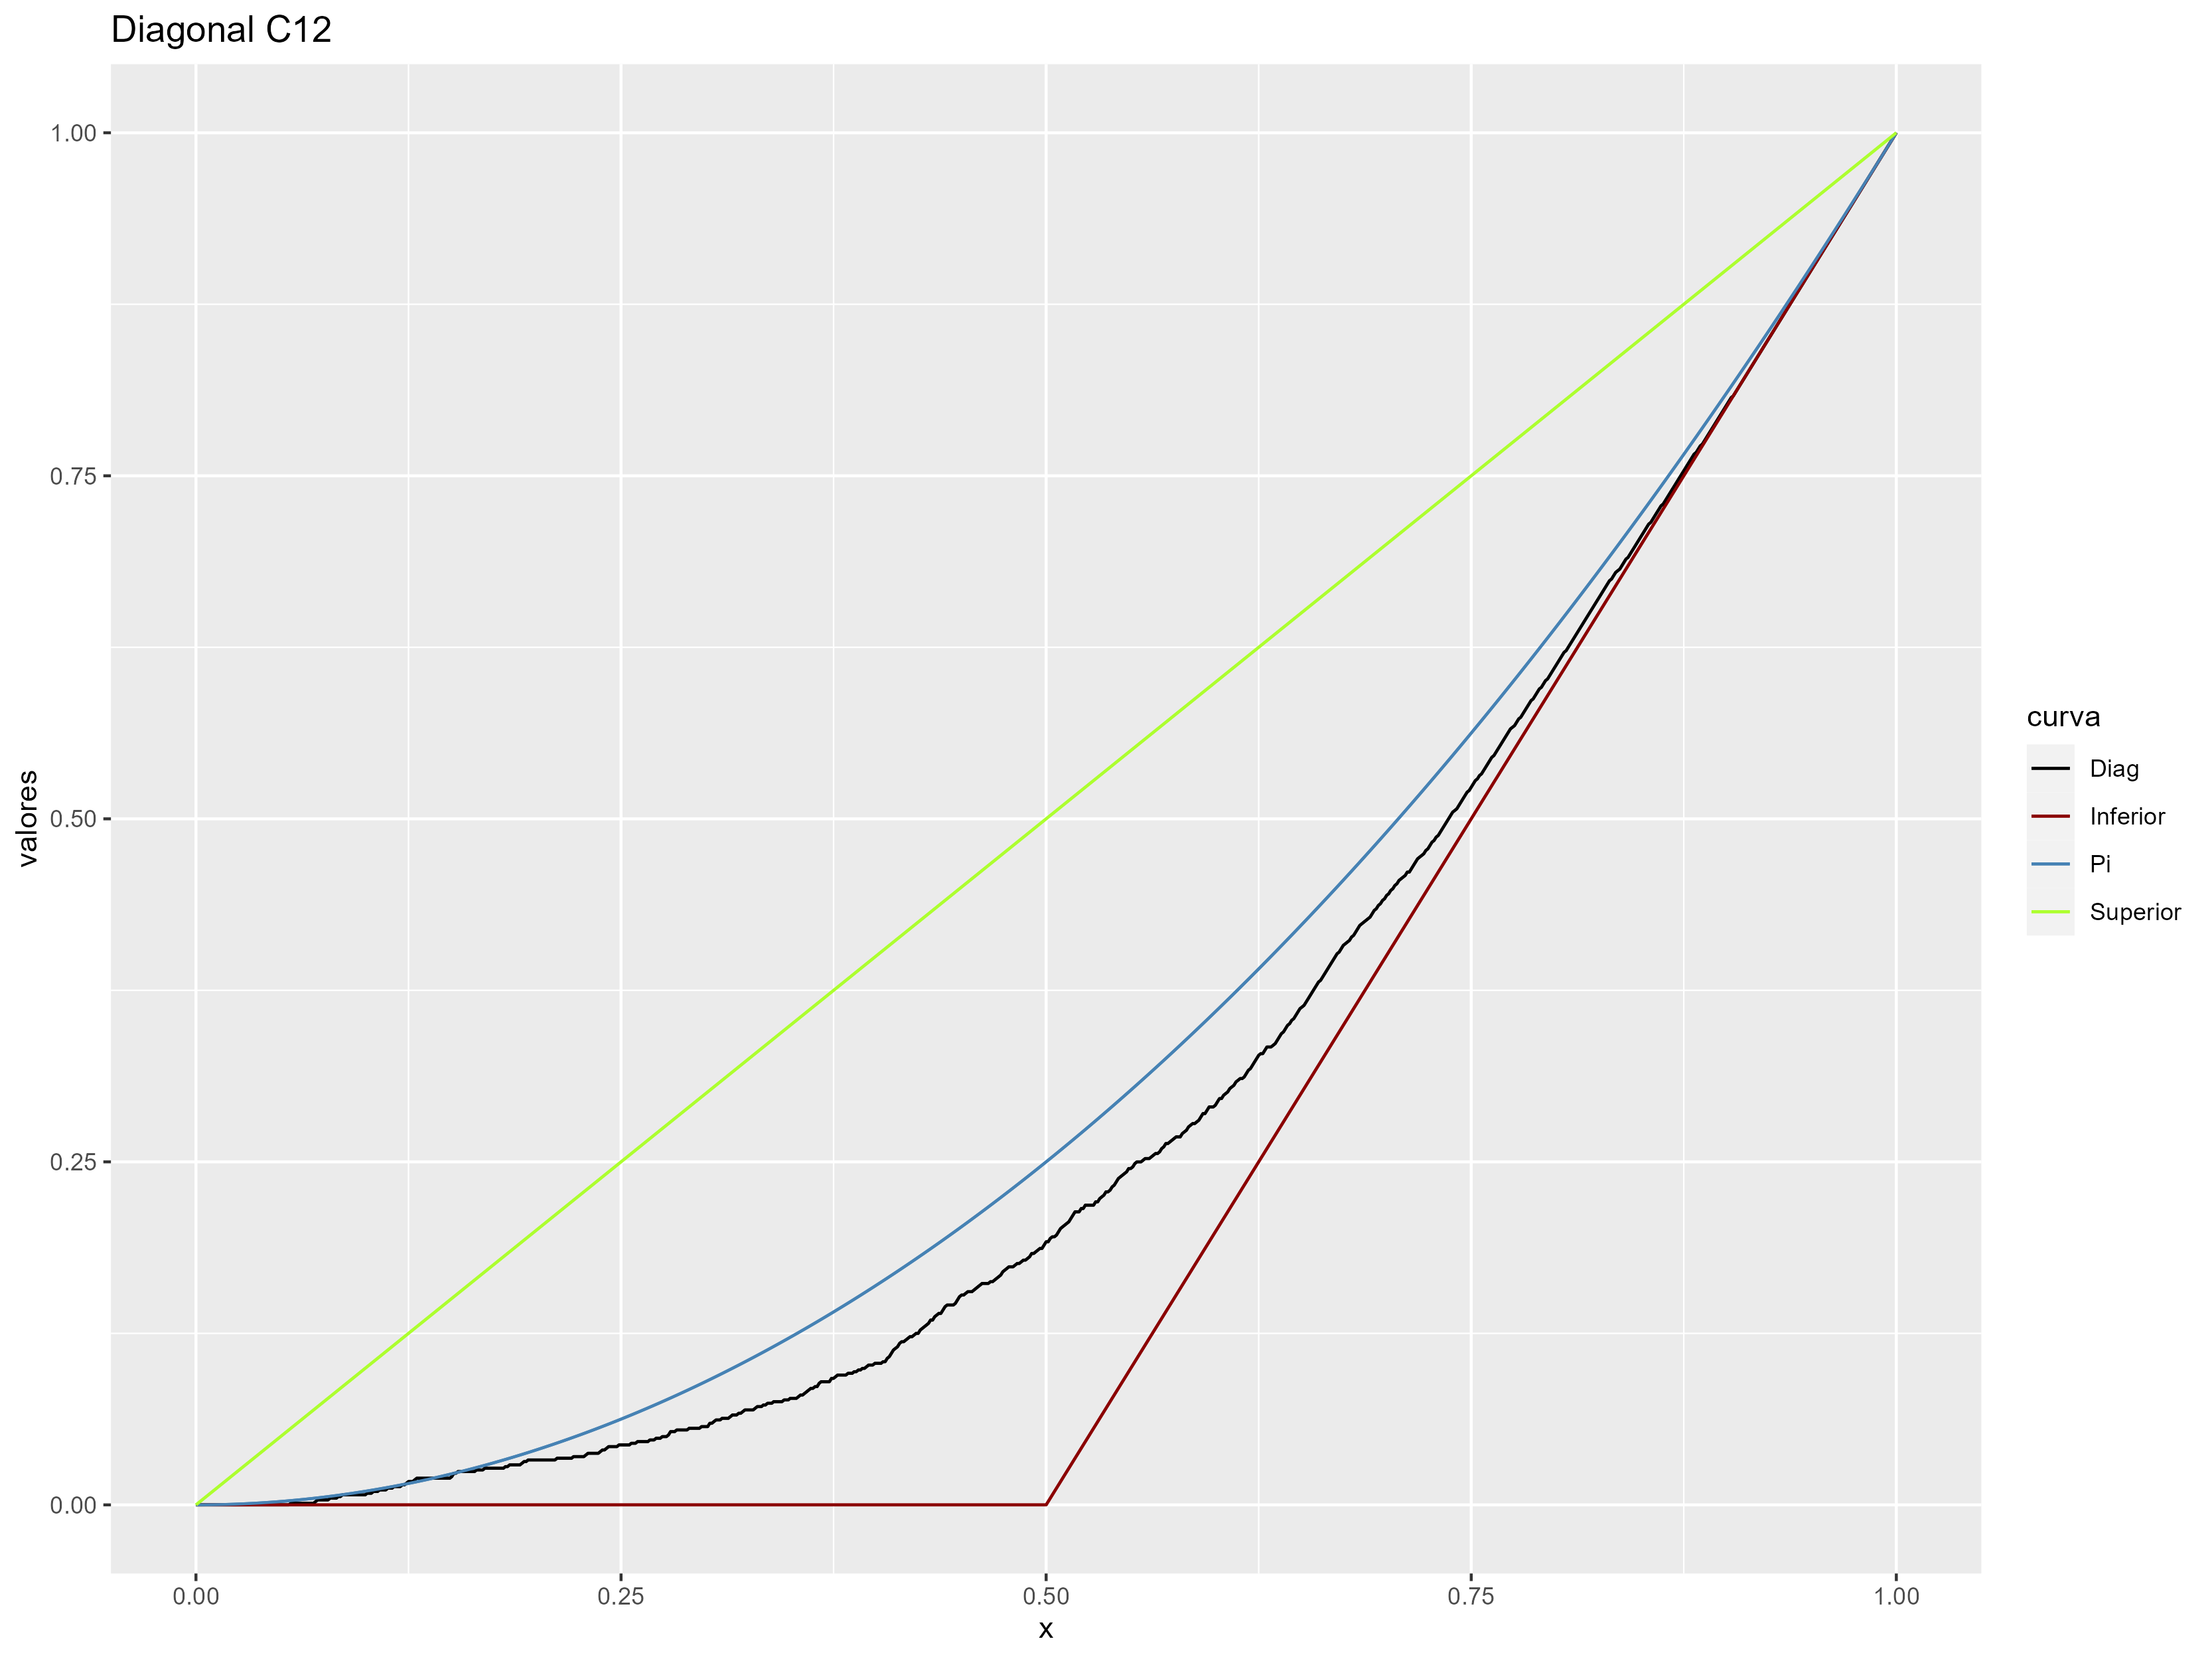
\includegraphics[width =  0.6 \textwidth]{4img/DiagMujC12.png}
    \caption{Ejemplo de la visualización de las diagonales.}
    \label{fig:diagEj}
\end{figure}

Si la cópula es monótona a lo largo de la diagonal, significa que la asociación entre las variables aumenta o disminuye de manera constante a medida que ambas variables aumentan o disminuyen en valor. Esto indica una relación de dependencia monótona entre las variables. \cite{TesisEmanuel}

Para ilustrar cómo se interpretan las diagonales de las cópulas, en la Figura \ref{fig:diagEj}, se muestran varias diagonales de referencia: en azul, la diagonal de la cópula producto o independiente; en verde, la diagonal de la cópula $M$, que es la cota superior; y en rojo, la diagonal de la cópula $W$, que es la cota inferior. En negro se muestra la diagonal de la cópula empírica. Las tres primeras diagonales sirven como referencias para inferir la relación que representa la cópula empírica.

\begin{itemize}
    \item Si la diagonal de la cópula empírica es muy cercana a la diagonal de la cópula independiente, es muy probable que no pase el test de independencia. En caso de que solo una sección de la diagonal de la cópula empírica sea cercana a la de la cópula independiente, se debería considerar la posibilidad de modelar esta relación utilizando una combinación de cópulas. Es decir, una sección se modelaría como una estructura independiente y la otra sección con una cópula diferente.

    \item Por otra parte, si la diagonal de la cópula empírica se encuentra por encima o por debajo de la diagonal de la cópula independiente, esto proporciona información sobre la naturaleza de la relación de monotonía entre las variables. Si está por encima, indica una relación monótona creciente, mientras que si está por debajo, sugiere una relación monótona decreciente. Del mismo modo, esta interpretación puede aplicarse a secciones específicas de la cópula.
\end{itemize}

En la Figura \ref{fig:diagEj}, se puede observar una cópula cuya relación es monótona decreciente en todo el dominio. Además, parece haber secciones donde se encuentra muy cerca de la cópula independiente en los extremos. La noción de cercanía es meramente intuitiva, por lo que este análisis es una herramienta de carácter exploratorio.

Estudiar las secciones diagonal, horizontal y vertical de una cópula en términos de relaciones monótonas, ayuda comprender mejor la dirección y la fuerza de la dependencia entre las variables aleatorias en diferentes escenarios. 



%%%%%%%%%%%%%%%%%%%%%%%%%%%%%%%%%%%%%%%%%%%%%%%%%%%%%
%%%%%%%%%%%%% pares de Copulas %%%%%%%%%%%%%%%%%%%%%%

\section{Cópulas Paramétricas}

Hay variables aleatorias paramétricas, como las distribuciones normales o gamma, poseen una forma específica definida por sus parámetros, lo que facilita su modelado y análisis en diferentes contextos. De manera similar, en el ámbito de las copulas, las copulas paramétricas ofrecen una herramienta poderosa para 
representar la estructura de dependencia entre variables aleatorias. Al ajustar los parámetros de la copula, es posible capturar una amplia gama de patrones de dependencia, desde la independencia hasta la dependencia extrema. 

Este enfoque paramétrico proporciona flexibilidad en la modelización de relaciones complejas entre variables, lo que resulta especialmente útil. En la modelización de variables aleatorias individuales como en la descripción de su dependencia conjunta, el uso de funciones paramétricas es de gran útilidad para capturar con precisión la variabilidad y las interacciones en los datos. En la Figura \ref{fig:Parametric}\footnote{Figura tomada de \cite{ImgCopulas}} se muestran las curvas de nivel de algunas cópulas paramétricas.

\begin{figure}[H]
    \centering
    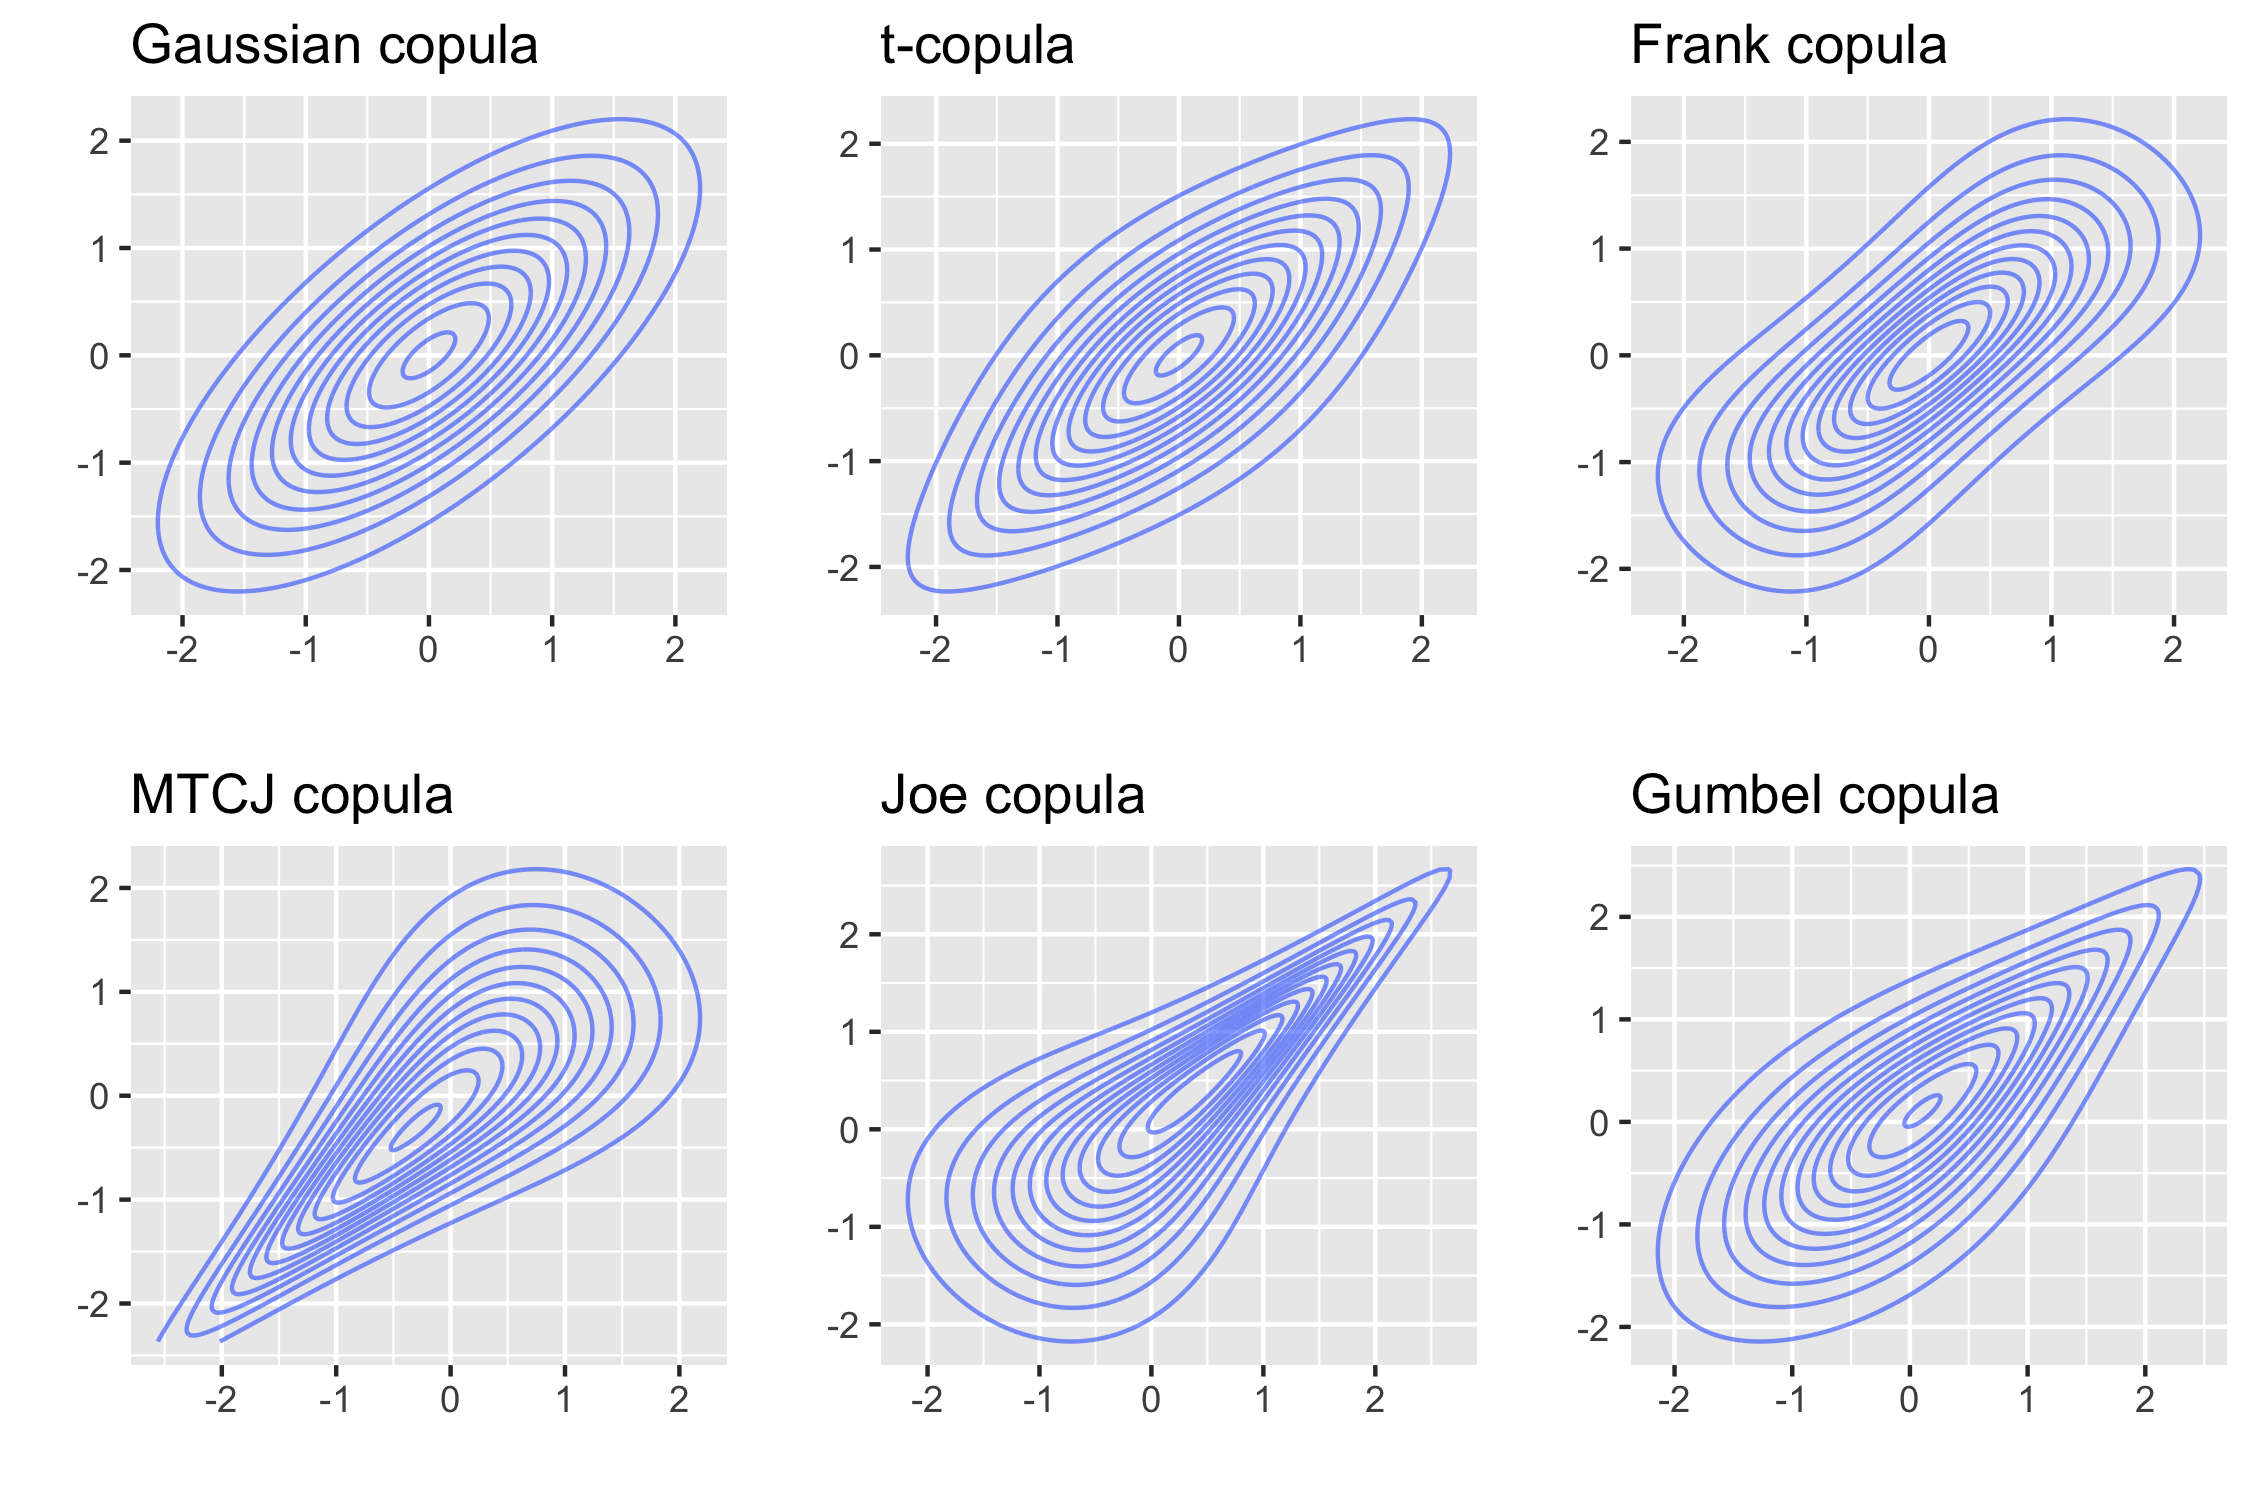
\includegraphics[width = 0.7 \textwidth]{Imagenes/parametricCopulas.png}
    \caption{Ejemplos de Cópulas para Paramétricas.}
    \label{fig:Parametric}
\end{figure}

\begin{ejemplo}[Distribución éstandar Bivariada $t$ de Student] La Distribución éstandar Bivariada $t$ de Student, cuyo vector de media $\boldsymbol{\mu}$ es igual a cero, y la matriz de parámetros de escala es

\begin{equation}
    \Sigma_\rho=\left[\begin{array}{ll}
    1 & \rho \\
    \rho & 1
    \end{array}\right] .
\end{equation}

La densidad asociada esta dada por

\begin{equation}
    t\left(x_1, x_2 ; \nu, \rho\right)=\frac{\Gamma\left(\frac{\nu+2}{2}\right)\left(1-\rho^2\right)^{-1 / 2}}{\Gamma\left(\frac{\nu}{2}\right)(\nu \pi)}\left\{1+\frac{1}{\nu} \frac{x_1^2-2 x_1 x_2 \rho+x_2^2}{1-\rho^2}\right\}^{-\frac{v+2}{2}} .
\end{equation}
\end{ejemplo}

La biblioteca VineCopula es una herramienta poderosa y versátil para el modelado de dependencias multivariadas mediante cópulas en el entorno de R. Esta biblioteca proporciona una amplia variedad de familias paramétricas de cópulas que pueden ser utilizadas para capturar diferentes tipos de relaciones de dependencia entre variables aleatorias. A continuación, se muestra una tabla con las familias disponibles:

\begin{table}[H]
    \centering
    \begin{tabular}{||c|c|c|c||}
    \hline\hline
\textbf{Copula family}	       & \textbf{family}    & \textbf{par}	    & \textbf{par2}      \\\hline
Gaussian	                                & 1	        & (-1, 1)	& -         \\
Student t	                                & 2	        & (-1, 1)	& (2,Inf)   \\
(Survival) Clayton	                        & 3, 13	    & (0, Inf)	& -         \\
Rotated Clayton (90 and 270 degrees)	    & 23, 3     & (-Inf, 0)	& -         \\
(Survival) Gumbel	                        & 4, 14	    & [1, Inf)	& -         \\
Rotated Gumbel (90 and 270 degrees)	24,     & 34	    & (-Inf, -1]& -         \\
Frank	                                    & 5	        & R \ {0}	& -         \\
(Survival) Joe	                            & 6, 16	    & (1, Inf)	& -         \\
Rotated Joe (90 and 270 degrees)	        & 26, 36    & (-Inf,-1)	& -         \\
(Survival) Clayton-Gumbel (BB1)	            & 7, 17	    & (0, Inf)	& [1, Inf)  \\
Rotated Clayton-Gumbel (90 and 270 degrees)	& 27, 37	& (-Inf, 0)	& (-Inf, -1]\\
(Survival) Joe-Gumbel (BB6)	                & 8, 18	    & [1 ,Inf)	& [1, Inf)  \\
Rotated Joe-Gumbel (90 and 270 degrees)	    & 28, 38	& (-Inf,-1]	& (-Inf, -1]\\
(Survival) Joe-Clayton (BB7)	            & 9, 19	    & [1, Inf)	& (0, Inf)  \\
Rotated Joe-Clayton (90 and 270 degrees)	& 29, 39	& (-Inf,-1]	& (-Inf, 0) \\
(Survival) Joe-Frank (BB8)	                & 10, 20	& [1, Inf)	& (0, 1]    \\
Rotated Joe-Frank (90 and 270 degrees)	    & 30, 40	& (-Inf,-1] & [-1, 0)   \\
(Survival) Tawn type 1	                    & 104, 114	& [1, Inf)	& [0, 1]    \\
Rotated Tawn type 1(90 and 270 degrees)	1   & 24, 134	& (-Inf,-1]	& [0, 1]    \\
(Survival) Tawn type 2	                    & 204, 214	& [1, Inf)	& [0, 1]    \\ 
Rotated Tawn type 2 (90 and 270 degrees)	& 224, 234	& (-Inf,-1]	& [0, 1]    \\ \hline \hline
    \end{tabular}
    \caption{Familias de cópulas paramétricas con las que trabaja R.}
    \label{tab:family_set}
\end{table}

%%%%%%%%%%%%%%%%% D - VINE COPULAS %%%%%%%%%%%%%%%%%%

\section{Cópulas D-Vine}

Se va a explorar un enfoque de modelado que emplea cópulas a pares, teniendo en cuenta las dependencias condicionales. La idea central radica en descomponer la distribución conjunta en una sucesión de cópulas a pares, las cuales se aplican tanto a las variables originales como a las distribuciones condicionales. La gran mayoría esta subsección se baso en el artículo \textit{Pair-copula constructions of multiple dependence} \cite{PairCopula}.

Usando el resultado del Teorema de Sklar \ref{TeoSklar}, y la regla de la cadena se puede obtener la función de densidad conjunta $f$, para una $F$ absolutamente continua con densidades marginales $F_1, \dots, F_n$ estrictamente crecientes y continuas se tiene la igualdad de la ecuación \eqref{conjunta}. Para alguna única cópula de densidad de $d-$variedad. 

\begin{equation}\label{conjunta}
    f\left( x_1, \dots, x_n\right)=  c_{1 \cdots n} (F_1\left(x_1\right), \ldots, F_n\left(x_n\right) ) \cdot f_1\left(x_1\right) \dots \cdot f_n\left(x_n\right)
\end{equation}

En particular, para el caso de $d = 2$ la descomposión de cópula a pares se ve como en la Ecuación \eqref{eq1}.

\begin{equation} \label{eq1}
    \begin{split}
        f (x1, x2) & = c_{12}(F1(x1), F2(x2)) \cdot f_1(x_1) \cdot f_2(x_2) \\
      \Rightarrow f\left(x_1 | x_2\right) & = c_{12}(F_1\left(x_1\right), F_2\left(x_2\right)) \cdot f_1\left(x_1\right)
    \end{split}
\end{equation}

Para $3$ variables la descommposición queda como se muestra en la ecuación \eqref{3var}.

\begin{equation}\label{3var}
    \begin{split}
        f\left(x_1 \mid x_2, x_3\right) & = c_{13 \mid 2} (F\left(x_1 \mid x_2\right), F\left(x_3 \mid x_2\right) ) \cdot f\left(x_1 \mid x_2\right) \\
        f\left(x_1 \mid x_2, x_3\right) & = c_{13 \mid 2}(F\left(x_1 \mid x_2\right), F\left(x_3 \mid x_2\right)) \cdot c_{12}( F\left(x_1\right), F\left(x_2\right)) \cdot f_1(x_1)
    \end{split}
\end{equation}

En general, para un vector $v$ $d-$dimensional y denótese $v_j$ un elemento arbitrario de $v$ y $v_{-j}$ al vector $v \setminus \left\{ v_j \right\}$, se tiene la formula \eqref{fact}. Esta representa la formula de representar la distribución en términos de una copula a par.

\begin{equation}\label{fact}
    f(x \mid \boldsymbol{v}) = c_{x v_j \mid \boldsymbol{v}_{-j}} (  F \left(x \mid \boldsymbol{v}_{-j}\right), F\left(v_j \mid \boldsymbol{v}_{-j}\right) ) \cdot f\left(x \mid \boldsymbol{v}_{-j}\right)
\end{equation}

\begin{lema}[Densidades Condicionales y funciones de distribución de distribuciones bivariadas en términos de su cópula]La densidad condicional y la función de distribución puede ser reescrita como

\begin{equation}
    \begin{aligned}
    f_{1 \mid 2}\left(x_1 \mid x_2\right) & =c_{12}\left(F_1\left(x_1\right), F_2\left(x_2\right)\right) f_2\left(x_2\right) \\
    F_{1 \mid 2}\left(x_1 \mid x_2\right) & =\left.\frac{\partial}{\partial u_2} C_{12}\left(F_1\left(x_1\right), u_2\right)\right|_{u_2=F_2\left(x_2\right)} \\
    & =: \frac{\partial}{\partial F_2\left(x_2\right)} C_{12}\left(F_1\left(x_1\right), F_2\left(x_2\right)\right) .
    \end{aligned}
\end{equation}

Lema tomado de \cite[pag 20]{czadoAnalyzing}.
\end{lema}

Como notación estándar se denota a la función $h(x, v, \Theta)$ a distribución condicional cuando $x$ y $v$ con uniformes. 

\begin{equation}
    h(x, v, \Theta) = F(x \mid v)=\frac{\partial C_{x, v}(x, v, \Theta)}{\partial v}
\end{equation}
%%%%%%%%%%%%%%%%%%%%%%%%%%%%%%%%%%%%%%%%%%%%%%%%%

Considérese un vector aleatorio $X = (X_1, \dots, X_d)$ con función de densidad $f(x_1, \dots, x_d)$ esta función puede ser factorizada como se muestra en la Ecuación \eqref{fact1} y esta descomposición es única hasta una reorganización de las variables.

\begin{equation}\label{fact1}
    f(x_1, \dots, x_d) = f(x_d) \cdot f(x_{d-1}|x_d) \cdot f(x_{d-2} | x_{d-1}, x_{d}) \dots \cdot  f(x_{d-2} | x_{2}, \dots, x_{d-1}, x_{d})
\end{equation}

En el caso de distribuciones de alta dimensionalidad, surgen numerosas posibles descomposiciones a pares de cópulas. Bedford y Cooke introdujeron un modelo gráfico conocido como \textit{vine regular}. En particular, nos interesa una arquitectura específica llamada \textit{vine drawble} o \textit{D-vines}.

En una D-vine, las cópulas a pares se organizan en una estructura de árbol. Para construir una D-vine, las variables aleatorias se ordenan secuencialmente y se emparejan de manera que cada nodo tenga dos aristas o una sola arista, formando así un camino. Para ilustrar este proceso, se presenta en la Figura \ref{fig:Dvine5} (tomada de \cite{PairCopula}) este emparejamiento en el árbol $T_1$ con un ejemplo de 5 variables.

Se inicia asignando una cópula bivariada a cada par de variables adyacentes. Luego, cada cópula o arista se convierte en un nodo en el siguiente árbol, y nuevamente a cada arista se le asigna una cópula, pero esta vez condicionada por la variable presente en ambos nodos, como se muestra en el árbol $T_2$ de la Figura \ref{fig:Dvine5}. Este proceso de repite hasta que solo se tenga una arista la cual corresponde a la última cópula. 

\begin{figure}[H]
    \centering
    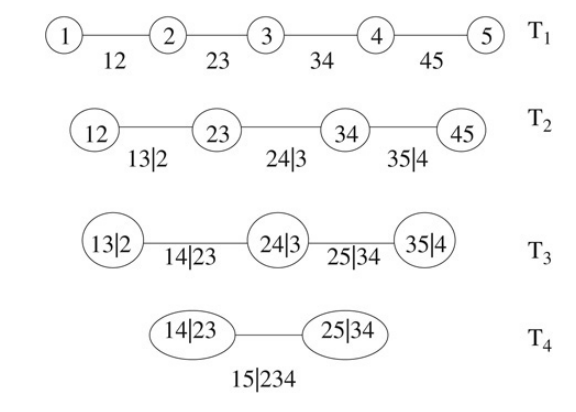
\includegraphics[width = 0.6 \textwidth]{Imagenes/Dvine5var.png}
    \caption{D-vine de 5 variables, 10 Aristas y 4 Arboles.}
    \label{fig:Dvine5}
\end{figure}

Al finalizar esta construcción, se obtiene una forma sencilla de visualizar la representación de la distribución conjunta utilizando cópulas a pares, como se muestra en la ecuación \eqref{dist5}. Los argumentos de las funciones cópula son distribuciones condicionales, en la ecuación \eqref{distC5} se muestra sus evaluaciones.

\begin{equation}\label{dist5}
     \begin{split}
         f(x_1, x_2, x_3, x_4, x_5) & = f(x_1) \cdot f(x_2) \cdot f(x_3) \cdot f(x_4) \cdot f(x_5)  \\
         & \cdot C_{12} \cdot C_{23} \cdot C_{34} \cdot C_{45} \quad (T_1)\\
         & \cdot C_{13|2} \cdot C_{24|3} \cdot C_{35|4} \quad (T_2)\\\
         & \cdot C_{14|23} \cdot C_{25|34} \quad (T_3)\\
         & \cdot C_{15|234} \quad (T_4)\\
     \end{split}
\end{equation}


\begin{equation}\label{distC5}
     \begin{split}
         f(x_1, x_2, x_3, x_4, x_5) & = f(x_1) \cdot f(x_2) \cdot f(x_3) \cdot f(x_4) \cdot f(x_5)  \\
         & \cdot C_{12}(F_1(x_1), F_2(x_2)) \cdot C_{23}(F_2(x_2), F_3(x_3)) \\
         & \cdot C_{34}(F_3(x_3), F_4(x_4)) \cdot C_{45}(F_4(x_4), F_5(x_5)) \quad (T_1)\\
         & \cdot C_{13|2}(F_{1|2}(x_1|x_2), F_{3|2}(x_3|x_2)) \cdot C_{24|3}(F_{2|3}(x_2|x_3), F_{4|3}(x_4|x_3))\\
         &\cdot C_{35|4}(F_{3|4}(x_3|x_4), F_{5|4}(x_5|x_4)) \quad (T_2)\\
         & \cdot C_{14|23}(F_{1|23}(x_1|x_2, x_3), F_{4|23}(x_4|x_2, x_3)) \\
         & \cdot C_{25|34}(F_{2|34}(x_2|x_3, x_4), F_{5|34}(x_5|x_3, x_4)) \quad (T_3)\\
         & \cdot C_{15|234}(F_{1|234}(x_1|x_2, x_3, x_4), F_{5|234}(x_5|x_2, x_3, x_4)) \quad (T_4)\\
     \end{split}
\end{equation}
  %%%%%%%%%%%%%%%%%%%%%%%%%%%%%%%%%%%%%%%%%%%%%%%%%%%%%%
  %%%%%%%%%%%%%%   R E G R E S I O N   %%%%%%%%%%%%%%%%%
  %%%%%%%%%%%%%%%%%%%%%%%%%%%%%%%%%%%%%%%%%%%%%%%%%%%%%%

\section{Regresión Cuantílica Usando D-Vines}

Como es típico en los métodos de regresión, el objetivo principal es comprender o predecir la variable respuesta $Y$ a partir de las covariables $X_1, X_2, \dots , X_d$.

\begin{equation}\label{regresion}
    y = \Phi_{\alpha}(x)
\end{equation}

Qué es la solución de 

\begin{equation}
     \mathbb{P}[Y \leq y | X_1 = x_1, \dots, X_n = x_n ] = \alpha
\end{equation}

Ejemplo de la solución para una covariable

\begin{equation}
    F_{y|x}(y|x) = \frac{\partial }{\partial u_x} C_{yx}(F_y(y), u_x) \Big|_{u_x = F_x(x)}  
\end{equation}

En general, 

\begin{equation}
    F_{y|\overline{x}}(y|\overline{x}) = \frac{\partial }{\partial u_{\overline{x}}} C_{y\overline{x}}(F_y(y), u_{\overline{x}}) \Big|_{u_{\overline{x}} =F_{\overline{x}(x)}} 
\end{equation}

Ejemplo de regresión con 3 variables 

\begin{equation}
    \begin{aligned}
    C_{V \mid U_1, U_2, U_3}\left(v \mid u_1, u_2, u_3\right) 
    = & h_{V \mid U_3 ; U_1, U_2}\left(C_{V \mid U_1, U_2}\left(v \mid u_1, u_2\right) \mid C_{U_3 \mid U_1, U_2}\left(u_3 \mid u_1, u_2\right)\right) \\
    = & h_{V \mid U_3 ; U_1, U_2}\left(h_{V \mid U_2 ; U_1}\left(C_{V \mid U_1}\left(v \mid u_1\right) \mid C_{U_2 \mid U_1}\left(u_2 \mid u_1\right)\right) \mid\right. \\
    & \left.h_{U_3 \mid U_1 ; U_2}\left(C_{U_3 \mid U_2}\left(u_3 \mid u_2\right) \mid C_{U_1 \mid U_2}\left(u_1 \mid u_2\right)\right)\right) \\ 
    = & h_{V \mid U_3 ; U_1, U_2}\left(h_{V \mid U_2 ; U_1}\left(h_{V \mid U_1}\left(v \mid u_1\right) \mid h_{U_2 \mid U_1}\left(u_2 \mid u_1\right)\right) \mid\right. \\
    & \left.h_{U_3 \mid U_1 ; U_2}\left(h_{U_3 \mid U_2}\left(u_3 \mid u_2\right) \mid h_{U_1 \mid U_2}\left(u_1 \mid u_2\right)\right)\right).
    \end{aligned}
\end{equation}


Después de haber ilustrado el funcionamiento con un pequeño ejemplo de tres variables, el siguiente paso será proporcionar una descripción exhaustiva de la implementación del algoritmo disponible en GitHub \url{https://github.com/BesitosDeBaba/deerVineReg}.

%%%%%%%%%%%%%%%%%%%%%%%%%%%%%%%%%%%%%%%%%%%%%%%%%
%%%%%%%%%% G R A F O  I N I C I A L  %%%%%%5%%%%%
%%%%%%%%%%%%%%%%%%%%%%%%%%%%%%%%%%%%%%%%%%%%%%%%%
\section{Descripción de la Implementación Computacional}

A continuación, se abordarían aspectos como los algoritmos utilizados para el ajuste de cópulas, las técnicas de optimización para la estimación de parámetros y las estrategias para la validación del modelo. 

\subsection{Formación del Grafo Inicial}

El programa ofrece dos opciones para construir el grafo inicial:

\begin{enumerate}
    \item \textbf{Construir el árbol}. Se basa en utilizar la medida de dependencia de $\sigma$ Schweizer y Wolff, en su forma empírica como se mostró en ecuación \eqref{SWEemp}. Por lo tanto, para iniciar el algoritmo, es necesario calcular la matriz que contenga la dependencia $\sigma$ entre todas las variables a la cual se le llamará $\Sigma$.

    En el algoritmo \ref{algT1}, se describe la formación del primer árbol.

    \item \textbf{Especificar el árbol}. La segunda opción consiste en introducir manualmente la secuencia a través del entorno de fórmulas de R, donde se especifica la relación deseada entre las variables. Por ejemplo, $Y \sim x_1 + x_2 + x_3$. Este enfoque se utiliza con el propósito de establecer la relación deseada, especialmente desde un punto de vista médico o  por cuestiones experimentales.
\end{enumerate}

\begin{algorithm}[H]
      \caption{Arból Inicial}
      \label{algT1}
      \begin{algorithmic}[1]  
        \Require{Matriz de dependencia $\Sigma$; número total de variables (contando la variable respuesta) $n$}
        \Ensure{Formación del árbol inicial.}
        
        \State $i = 1$
        \State Asignar al nodo actual la variable respuesta, $Nodo_{actual}$.
        
        \While{$i < N$ \do}
          \State Buscar en la columna o renglón del nodo actual el nodo con la dependencia más alta, llamesé $Nodo_{nuevo}$.
          \State Unir $Nodo_actual$ con $Nodo_{nuevo}$.
          \State Actualizar $Nodo_{actual}$ con $Nodo_{nuevo}$.     
          \State{i=i+1}
        \EndWhile
       
    \State{\textbf{Output:} Devolver el grafo.}
      \end{algorithmic}
    \end{algorithm}

%%%%%%%%%%%%%%%%%%%%%%%%%%%%%%%%%%%%%%%%%%%%%%%%%
%%%%%%%%%%%%%% F O R W A R D  %%%%%%%%%%%%%5%%%%%
%%%%%%%%%%%%%%%%%%%%%%%%%%%%%%%%%%%%%%%%%%%%%%%%%

\subsection{Forward}

El siguiente paso consiste en estimar las cópulas utilizando la función \textit{BiCopSelect}. En este proyecto, nos centraremos exclusivamente en el ajuste de cópulas perimétricas; las razones de esta elección se explicarán en el próximo capítulo. Además, para calcular las funciones de distribución condicionales, o su equivalente, la derivada de cópula como se muestra en la ecuación \eqref{fact}, se utilizará la función \textit{BiCopHfunc2}, ambas disponibles en la biblioteca de R, \textbf{VineCopula} para más detalles de implementación ver \url{https://cran.r-project.org/web/packages/VineCopula/index.html}. Es necesario calcular las funciones $h$ en cada nivel para completar la etapa de avance (forward). Estas funciones $h$ serán necesarias para la etapa de retroceso (backward) y para realizar predicciones precisas.

La transformación a escala $u$ hace referencia a convertir las variables aleatorias marginales en distribuciones uniformes en el intervalo $[0, 1]$, es necesaria para trabajar con cópulas. Se realiza aplicando la función de distribución acumulativa empírica de cada variable aleatoria como se describe en \eqref{fdaEmp}.

Adicionalmente, de acuerdo al paquete \textit{VineCopula}, las cópulas son seleccionadas usando \textit{Akaike} y \textit{Bayesian Information Criteria} (AIC y BIC), los cuales están definidos en las ecuaciones \ref{AIC} y \ref{BIC} respectivamente. Inicialmente, todas las cópulas disponibles se ajustan utilizando la estimación de máxima verosimilitud. Luego, se calculan los criterios para todas las familias de cópulas disponibles y se elige la familia con el valor mínimo.

\begin{equation}\label{AIC}
    AIC := -2 \sum_{i=1}^N \ln[c(u_{i,1},u_{i,2}|\boldsymbol{\theta})] + 2k,
\end{equation}

Donde $k$ es igual a $1$ para cópulas de un parámetro y $k$ es igual a $2$ para cópulas de dos parámetros como las cópulas t-, BB1, BB6, BB7 y BB8.

\begin{equation}\label{BIC}
    BIC := -2 \sum_{i=1}^N \ln[c(u_{i,1},u_{i,2}|\boldsymbol{\theta})] + \ln(N)k.
\end{equation}

Notesé que el BIC penaliza más fuerte a las familias de dos parámetros que el AIC.

En la Algoritmo \ref{algfordward} se describe detalladamente el proceso de ajuste de cada cópula utilizada en la D-vine y en la Figura \ref{fig:construccion} se muestra un diagrama que representa como se ejecuta este ajuste.

\begin{algorithm}[H]
      \caption{Forward}
      \label{algfordward}
      \begin{algorithmic}[1]  
        \Require{Data frame con los observaciones en el orden que dicto el algoritmo anterior, $data$: número de variables $n$.}
        \Ensure{Estimación de las cópulas y las funciones $h$.}

        \State $copulas =  \left [  \right ]$; $hs =  \left [  \right ]$; $niveles = n-1$
        
        \State Obtener la función de distribución empírica de cada variable y posteriormente cada una transfórmala a escala $u$, con su respectiva función de distribución. 
        \State Asignar a $dataU$ los datos en escala $u$.
        
        \State $i = 1$
        \While{$i \leq niveles$ \do}
          \State Estimar cada cópula con la función $BiCopSelect$ de $R$. Para $i = 1$ los argumentos corresponde la datos de $dataU$, para los otros casos corresponden a funciones $h$.
          \State Calcular las funciones $h$ de cada cópula para el siguiente nivel.
          \State Añadir las copulas en $copulas$.
          \State Añadir las funciones $h$ a $hs$.
          \State{i=i+1}
        \EndWhile
       
    \State{\textbf{Output:} Devolver $copulas$ y $hs$.}
      \end{algorithmic}
    \end{algorithm}



Después de realizar el ajuste, como era de esperar, se desea evaluar la existencia de la dependencia modelada. Para determinar si hay independencia entre las variables, es decir, si las cópulas que modelan la dependencia entre ellas pueden simplificarse a la cópula independiente, se emplea la estadística descrita en la ecuación \eqref{T} para realizar el test de independencia implementado en \textbf{VineCopula}.
    
\begin{equation}\label{T}
    T = \sqrt{\frac{9N(N - 1)}{2(2N + 5)}} \times |\hat{\tau}|,
\end{equation}

Donde $N$ es el número de observaciones y $\hat{\tau}$ es el tau de Kendall empírica de los vectores de datos $u_1$ u $u_2$. El valor p de la hipótesis nula de independencia bivariada.

\begin{equation}
    \texttt{p.value} = 2 \times \left(1 - \Phi\left(T\right)\right),
\end{equation}


Donde $\Phi$ es la función de distribución normal estándar.

\begin{figure}[H]
    \centering
    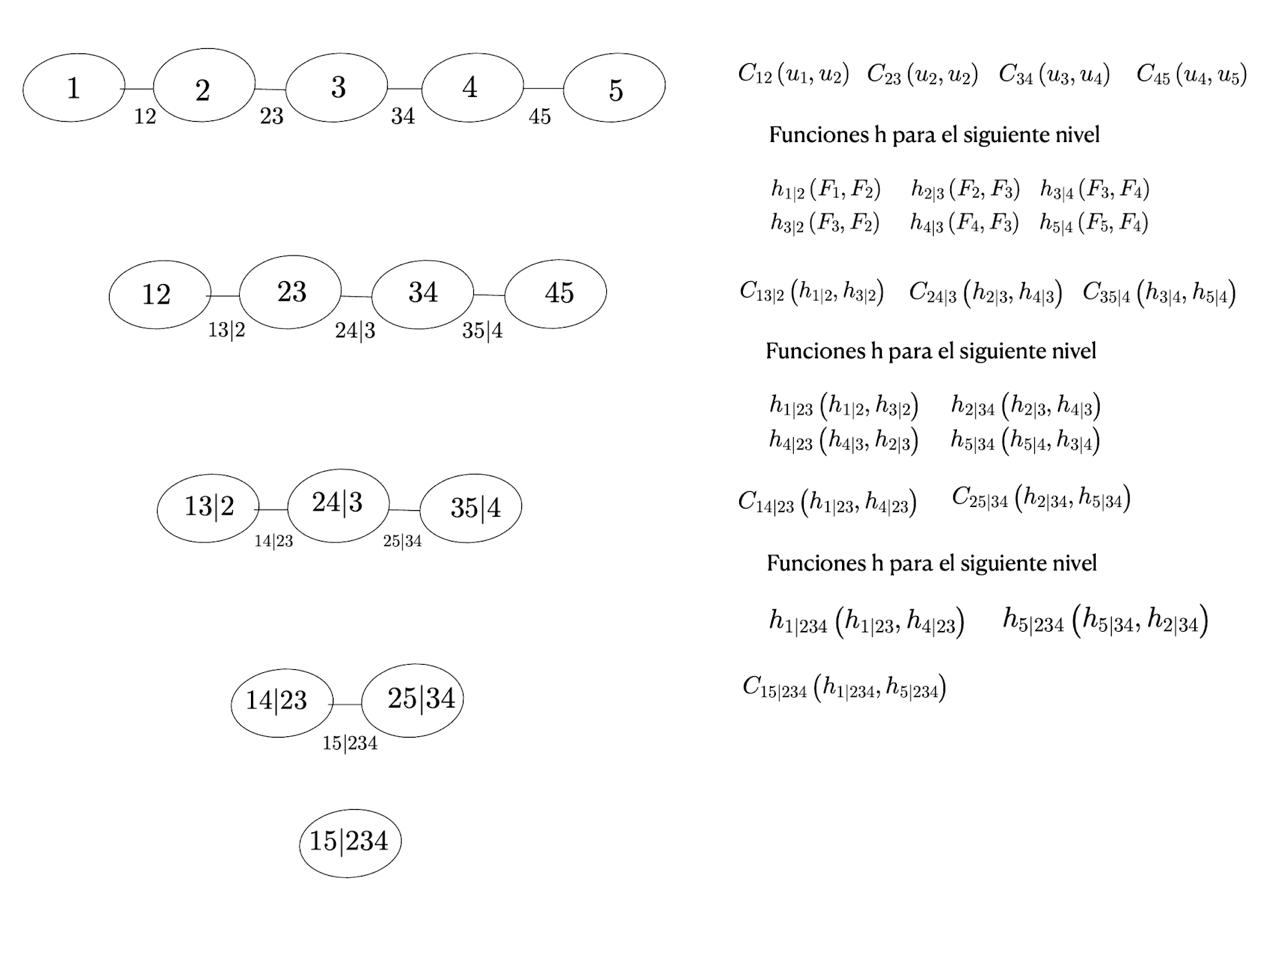
\includegraphics[width = 0.98\textwidth]{Imagenes/Construccion.jpeg}
    \caption{Visualización gráfica}
    \label{fig:construccion}
\end{figure}

%%%%%%%%%%%%%%%%%%%%%%%%%%%%%%%%%%%%%%%%%%%%%%%%%
%%%%%%%%%%%%%% F O R W A R D  %%%%%%%%%%%%%5%%%%%
%%%%%%%%%%%%%%%%%%%%%%%%%%%%%%%%%%%%%%%%%%%%%%%%%

\subsection{Backward}

Una vez estimadas las cópulas y las funciones $h$  en cada nivel del árbol de cópulas, Ahora, se tiene que realizar las predicciones sobre las variables aleatorias originales. No hay que olvidar que, hay que obtener las funciones inversas esto se hará usando la función \textit{BiCopHinv2} que viene implementada en la librería \textbf{VineCopula}. Cabe mencionar que el orden de los argumentos es importante ya que obtiene la inversa con respecto a la segunda entrada. Se da en pseudo código en el Algoritmo \ref{algbackward}.


\begin{algorithm}[H]
      \caption{Backward}
      \label{algbackward}
      \begin{algorithmic}[1]  
        \Require{Data frame con los observaciones obtenidas del forward, $dataU$; lista con las funciones $h$ ajustadas en el backward, $hs$ ; lista que contiene las copulas ajustadas en el forward,  $copulas$; nivel de confiabilidad; $\alpha$.}
        \Ensure{Regresión Cuantil.}
        \State{$alphas = rep(alpha, nrows(dataU))$}
        
        \State $i = 1$
        \While{$i \leq niveles$ \do}
          \State Usar $BiCopHinv2$ para cada cópula creada con usando sus respectivas funciones $h$ en la variable $aux$. En la primera iteración los argumentos corresponden al vector $alphas$ y $dataU$.
          \State Actualizar $alphas = aux$
          \State{i=i+1}
        \EndWhile
       
    \State{\textbf{Output:} Devolver $alphas$.}
      \end{algorithmic}
    \end{algorithm}

Al finalizar el proceso descrito, se obtienen las cópulas ajustadas, las cuales son fundamentales cuando se pretende que cualquier individuo pueda ingresar sus datos y recibir un pronóstico preciso. Estas cópulas ajustadas capturan la estructura de dependencia entre las variables de la base dada, lo que permite generar predicciones para nuevas observaciones. 
\cleardoublepage

\chapter{Resultados}\label{Resultados}

En este estudio, se analizan datos de pacientes con el objetivo de identificar y modelar la relación entre diversas variables clínicas y la resistencia a la insulina. Los datos recopilados incluyen medidas de glucosa en diferentes momentos, índices de masa corporal, niveles de presión arterial, entre otros. La adecuada interpretación y modelado de estos datos pueden proporcionar interpretaciones valiosas sobre el estado de salud de los pacientes. 

Se realizó un análisis exploratorio de los datos para entender mejor su distribución y las relaciones entre las variables. Posteriormente, se ajustaron varios modelos de regresión D-vine, que permiten capturar las complejas dependencias entre las variables. 

\section{Análisis Exploratorio}

La base de datos con la que se trabajó fue proporcianada por la Dra. Adriana Monroy. Esta conformada por 1697 pacientes con distintos diagnósticos (normal, prediabetes o diabetes). Las variables que conforman la base son las siguientes:

\begin{itemize}
    \item \textbf{Clave} - Clave asociada a cada paciente, variable de tipo categórica.
    \item \textbf{No.} - Número con el que se indica a cada paciente, variable del tipo categórica.
    \item \textbf{Género} - Variable de tipo categórica que indica el genero del individuo: es $0$ si es masculino y $1$ si es femenino.
    \item \textbf{Gluc-0} - Nivel de glucosa en la sangre en mg/dl al minuto $0$ para la prueba oral de tolerancia a la glucosa.
    \item \textbf{Gluc+30} - Nivel de glucosa en la sangre en mg/dl al minuto $30$ para la prueba oral de tolerancia a la glucosa.
    \item \textbf{Gluc+60} - Nivel de glucosa en la sangre en mg/dl al minuto $60$ para la prueba oral de tolerancia a la glucosa.
    \item \textbf{Gluc+90} - Nivel de glucosa en la sangre en mg/dl al minuto $90$ para la prueba oral de tolerancia a la glucosa.
    \item \textbf{Gluc+120} - Nivel de glucosa en la sangre en mg/dl al minuto $120$ para la prueba oral de tolerancia a la glucosa.
    \item \textbf{Ins-0} - Nivel de insulina en la sangre en mg/dl al minuto $0$ durante la prueba oral de tolerancia a la glucosa.
    \item \textbf{Ins+30} - Nivel de insulina en la sangre en mg/dl al minuto $30$ durante la prueba oral de tolerancia a la glucosa.
    \item \textbf{Ins+60} - Nivel de insulina en la sangre en mg/dl al minuto $60$ durante la prueba oral de tolerancia a la glucosa.
    \item \textbf{Ins+90} - Nivel de insulina en la sangre en mg/dl al minuto $90$ durante la prueba oral de tolerancia a la glucosa.
    \item \textbf{Ins+120} - Nivel de insulina en la sangre en mg/dl al minuto $120$ durante la prueba oral de tolerancia a la glucosa.
    \item \textbf{BMI} - Indice de masa corporal.
    \item \textbf{PA diast} - Presión arterial diastólica en milímetros de mercurio (mm Hg).
\end{itemize}

Los tipos de datos con los que se cuenta para enfrentar el problema son del tipo numérico, categórico y funcional. Los datos numéricos o escalares se pueden modelar como variable aleatoria que toma valores en los números reales. Por otro lado, los datos categóricos se pueden modelarse como una variable aleatoria discreta que toma valores en conjunto de  etiquetas. Finalmente, un dato funcional es un tipo de variable que evoluciona con el tiempo o su posición en el espacio. En tal caso, cada observación corresponde a una función que describe como una cantidad especifica cambia con respecto a otra; en nuestro caso, como los niveles de de glucosa e insulina cambian con el tiempo.

%%%%%%%%%%%%%%%%%%%%%%%%%%%%%%%%%%%%%%%%%%%%%%%%%%%%%%%%%%%%%

\subsection{Datos Faltantes}

Durante el análisis de datos es importante tener en cuenta la cantidad de datos faltantes, ya que esto puede influir negativamente durante el desarrollo del modelo, pues al tener una reducción de información esto reduce precisión y el poder de predicción del modelo e incrementar su variabilidad. En la práctica se utiliza la imputación de datos, la cual es una técnica estadística que sustituye los valores faltantes de una observación por otros que son simulados \cite{Imputacion}. En la Figura \ref{fig:Nas}, se puede ver una representación gráfica de la cantidad y posición de datos faltantes de cada variable.

\begin{figure}[H]
    \centering
    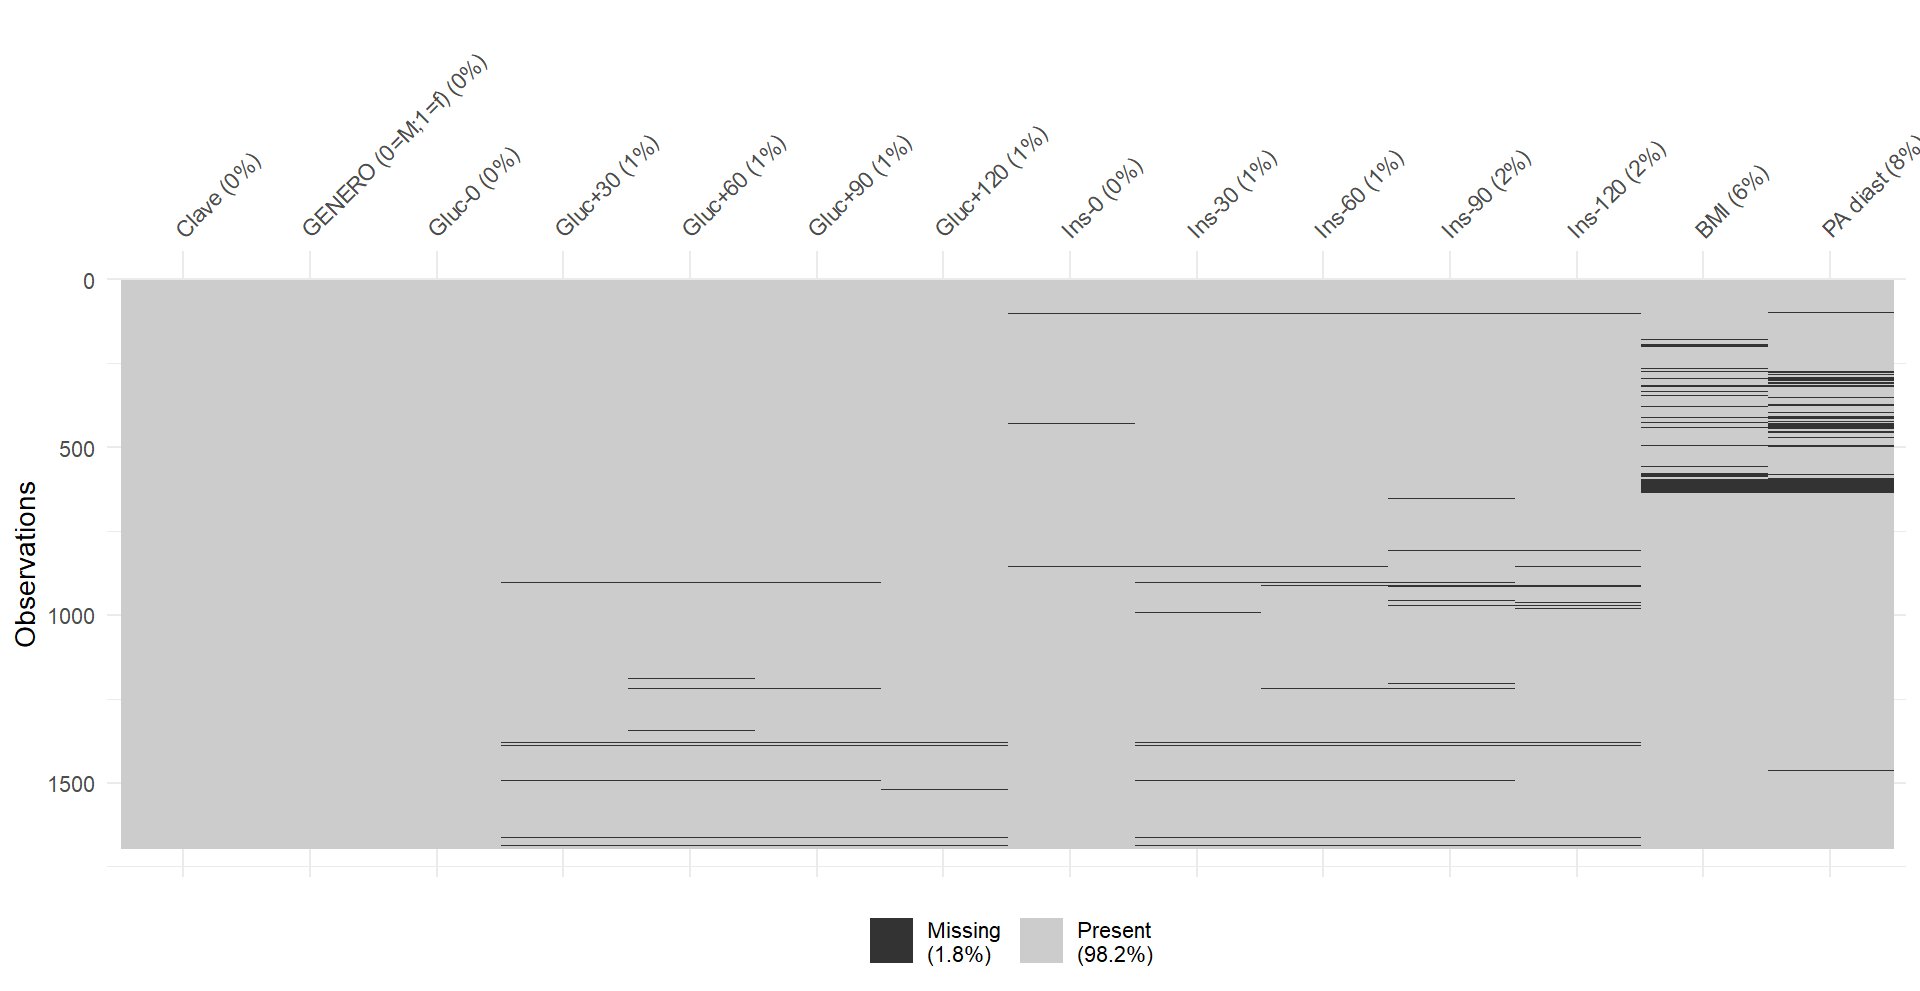
\includegraphics[width = 0.8 \textwidth, height = 6 cm]{Imagenes/datosFaltantes.png}
    \caption{Figura ilustrativa de los datos faltantes en la base de datos.}
    \label{fig:Nas}
\end{figure}

Para medir el nivel de datos faltantes de cada variable se toma la proporción de número de datos faltantes con respecto al total de datos. En el Cuadro \ref{tab:PorcentajeNA} se muestra el porcentaje de NA's de correspondiente a cada variable. Afortunadamente, esta cantidad no es mayor al $8 \%$; en casi todas las variables con datos faltantes esta cantidad es menor al $3\%$. 

\begin{table}[H]
\centering
\begin{tabular}{||c|c||c|c||}
\hline\hline
\textbf{Variable} & \textbf{\% de NA} & \textbf{Variable} & \textbf{\% de NA} \\ \hline\hline
PA diast          & 7.71950501        & BMI               & 6.01060695        \\ \hline
Ins-90            & 2.47495580        & Ins-120           & 2.23924573        \\ \hline
Ins-60            & 1.47318798        & Glu-90            & 1.41426046        \\ \hline
Glu-60            & 1.11962286        & Ins-30            & 1.06069534        \\ \hline
Glu-30            & 0.94284031        & Glu-120           & 0.64820271        \\ \hline
Ins-0             & 0.17678256        & -                 & -       \\ \hline\hline
\end{tabular}
\caption{Porcentaje de datos faltantes de cada variable.}
\label{tab:PorcentajeNA}
\end{table}

Considerando que el modelo estará especializado para su uso en el área médica y que la cantidad de datos faltantes no es excesiva, es preferible eliminar los individuos que contengan alguna covariable con valores faltantes (NA). Esto se debe a que utilizar técnicas de imputación puede alterar las relaciones estadísticas originales entre variables, afectando la capacidad del modelo para hacer inferencias válidas. En aplicaciones médicas, donde las decisiones basadas en el modelo pueden tener consecuencias significativas para la salud del paciente, es crucial mantener la precisión de estas inferencias. Además, la imputación puede distorsionar los patrones subyacentes en los datos, especialmente en conjuntos de datos médicos, donde las relaciones entre variables pueden ser complejas y no lineales, lo que puede llevar a modelos que no reflejen adecuadamente la realidad clínica.

\begin{figure}[H]
 \centering
  \subfloat[Mujeres]{
   \label{DatosFMu}
    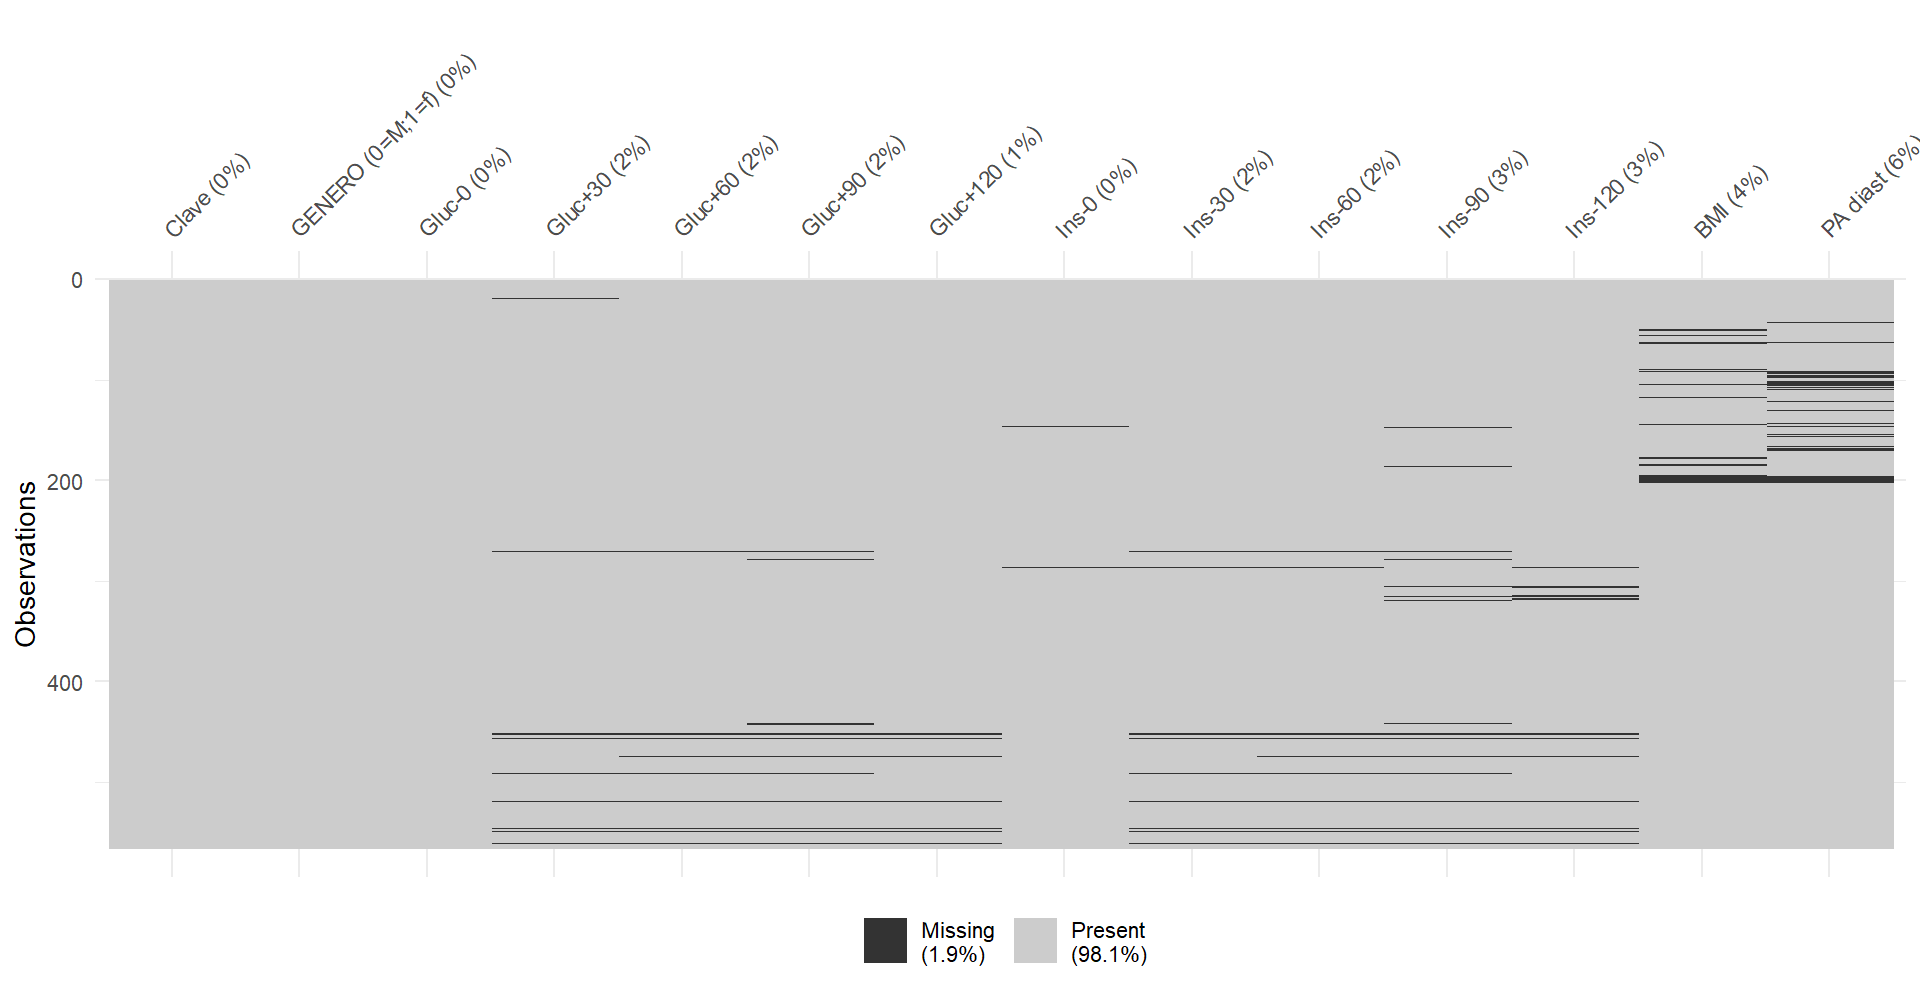
\includegraphics[width=0.45\textwidth]{Imagenes/datosFaltantesMujeres.png}}
  \subfloat[Hombres]{
   \label{Datos}
    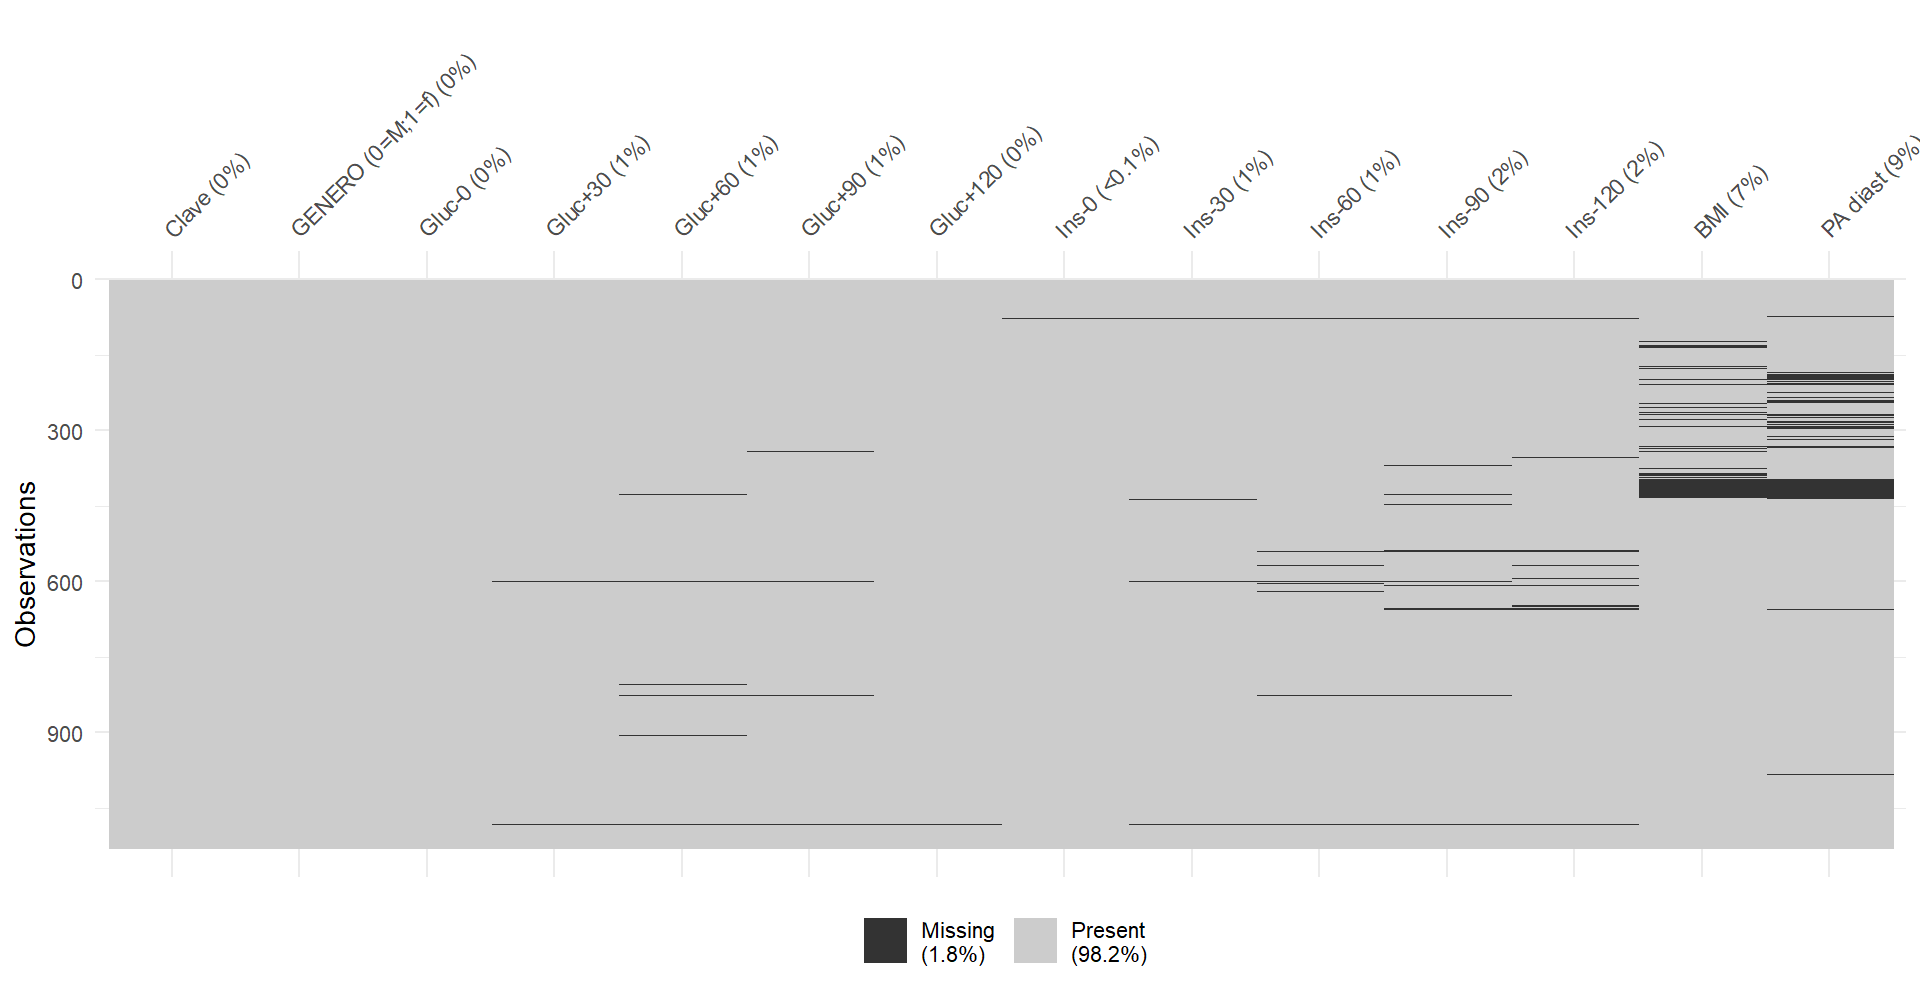
\includegraphics[width=0.45\textwidth]{Imagenes/datosFaltantesHombres.png}}
    \caption{Visualización de datos faltantes por género.}
    \label{fig:FaltantesGen}
\end{figure}

En la Figura \ref{fig:FaltantesGen}, se muestran los datos faltantes de acuerdo al género. En ambos géneros, las principales variables con datos faltantes son la presión diastólica y el índice de masa corporal. Sin embargo, la base de datos está desbalanceada en términos de género, con un total de $1131$ mujeres y $566$ hombres. Tener una base de datos desbalanceada puede presentar varias desventajas cuando se quieren implementar modelos por género. Como por ejemplo, puede causar que el modelo favorezca al grupo mayoritario, es decir, las predicciones y las inferencias serán más precisas para las mujeres en este caso, mientras que los hombres podrían no ser representados adecuadamente.

Después de remover los individuos que contienen alguna covariable con datos faltantes, la base de datos cuenta con un total de $1454$ individuos, de los cuales $956$ son mujeres y $498$ son hombres. Con este conjunto de datos se desarrollarán tres modelos: uno para la población en conjunto y dos modelos separados por género.

%%%%%%%%%%%%%%%%%%%%%%%%%%%%%%%%%%%%%%%%%%%%%%%%%%%%%%%%%%%%%%%%%%%%%
%%%%%%%%%%%%%%%%% 
%%%%%%%%%%%%%%%%%%%%%%%%%%%%%%%%%%%%%%%%%%%%%%%%%%%%%%%%%%%%%%%%%%%%%

\section{Visualización de Dependencias}

En algunas de las siguientes subsecciones se incluyen algunos otros estudios exploratorios. Por claridad y para hacer énfasis en su importancia, se decidió poner dichos análisis en subsecciones separadas. Para comenzar a analizar las dependencias entre las covariables, la Figura \ref{fig:corrSWE} presenta un mapa de calor elaborado con la matriz de correlación de Schweizer y Wolff, mientras que la Figura \ref{fig:corSpe} muestra un mapa de calor basado en la matriz de correlación de Spearman. Es importante recordar que el coeficiente de Spearman proporciona información sobre la dirección de la dependencia entre las variables. En la Figura \ref{fig:corSpe}, el mapa de calor revela que todas las dependencias identificadas son crecientes o positivas.

Adicionalmente, en el mapa de calor de la correlación de Schweizer y Wolff, se observa una dependencia significativa entre las mediciones de la curva de glucosa. Sin embargo, en cuanto a las mediciones de insulina, aunque las dependencias no son tan fuertes como las observadas en las variables de glucosa, siguen siendo considerables. Como se mencionó en el Capítulo \ref{insulina}, los niveles de insulina y glucosa en sangre durante la prueba oral de glucosa no son independientes. Sin embargo, las dependencias no son tan marcadas, aunque sí están presentes. 

\begin{figure}[H]
    \centering
    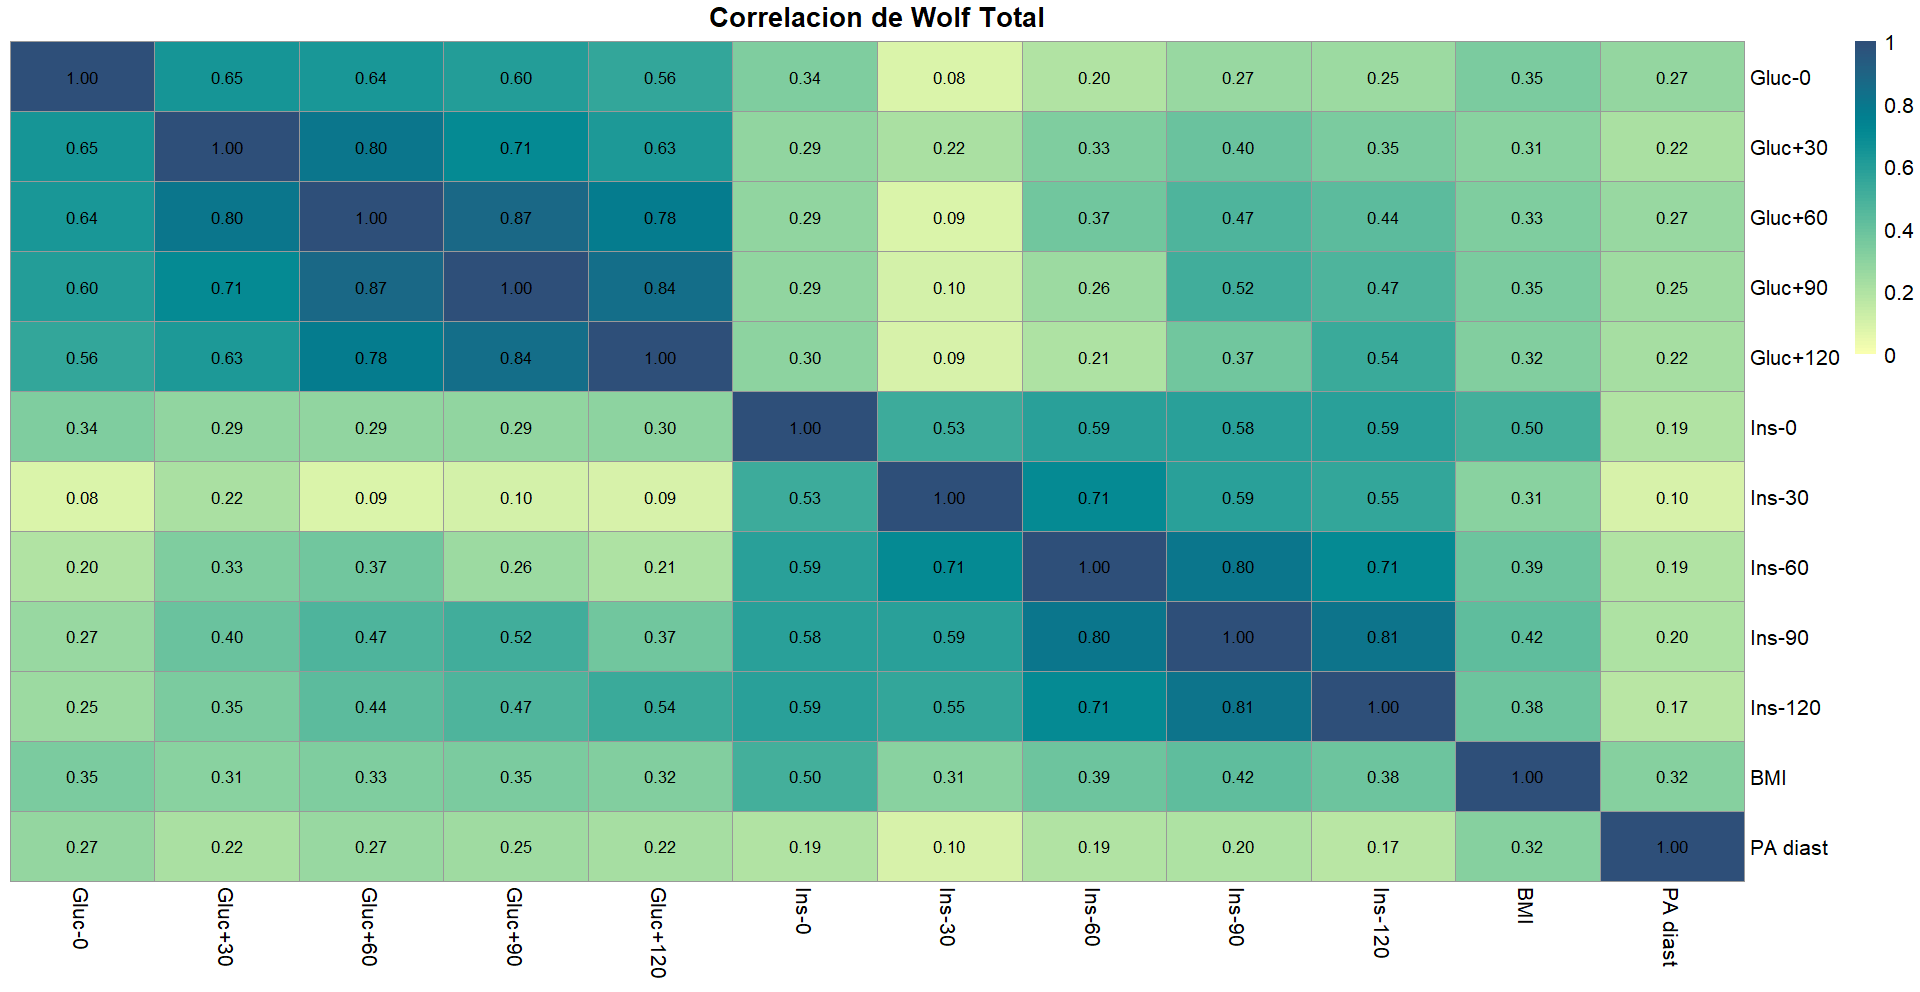
\includegraphics[width = 0.9 \textwidth]{Imagenes/corWolfTotal.png}
    \caption{Heatmap de las covariables numéricas con la correlación de Schweizer y Wolff.}
    \label{fig:corrSWE}
\end{figure}

\begin{figure}[H]
    \centering
    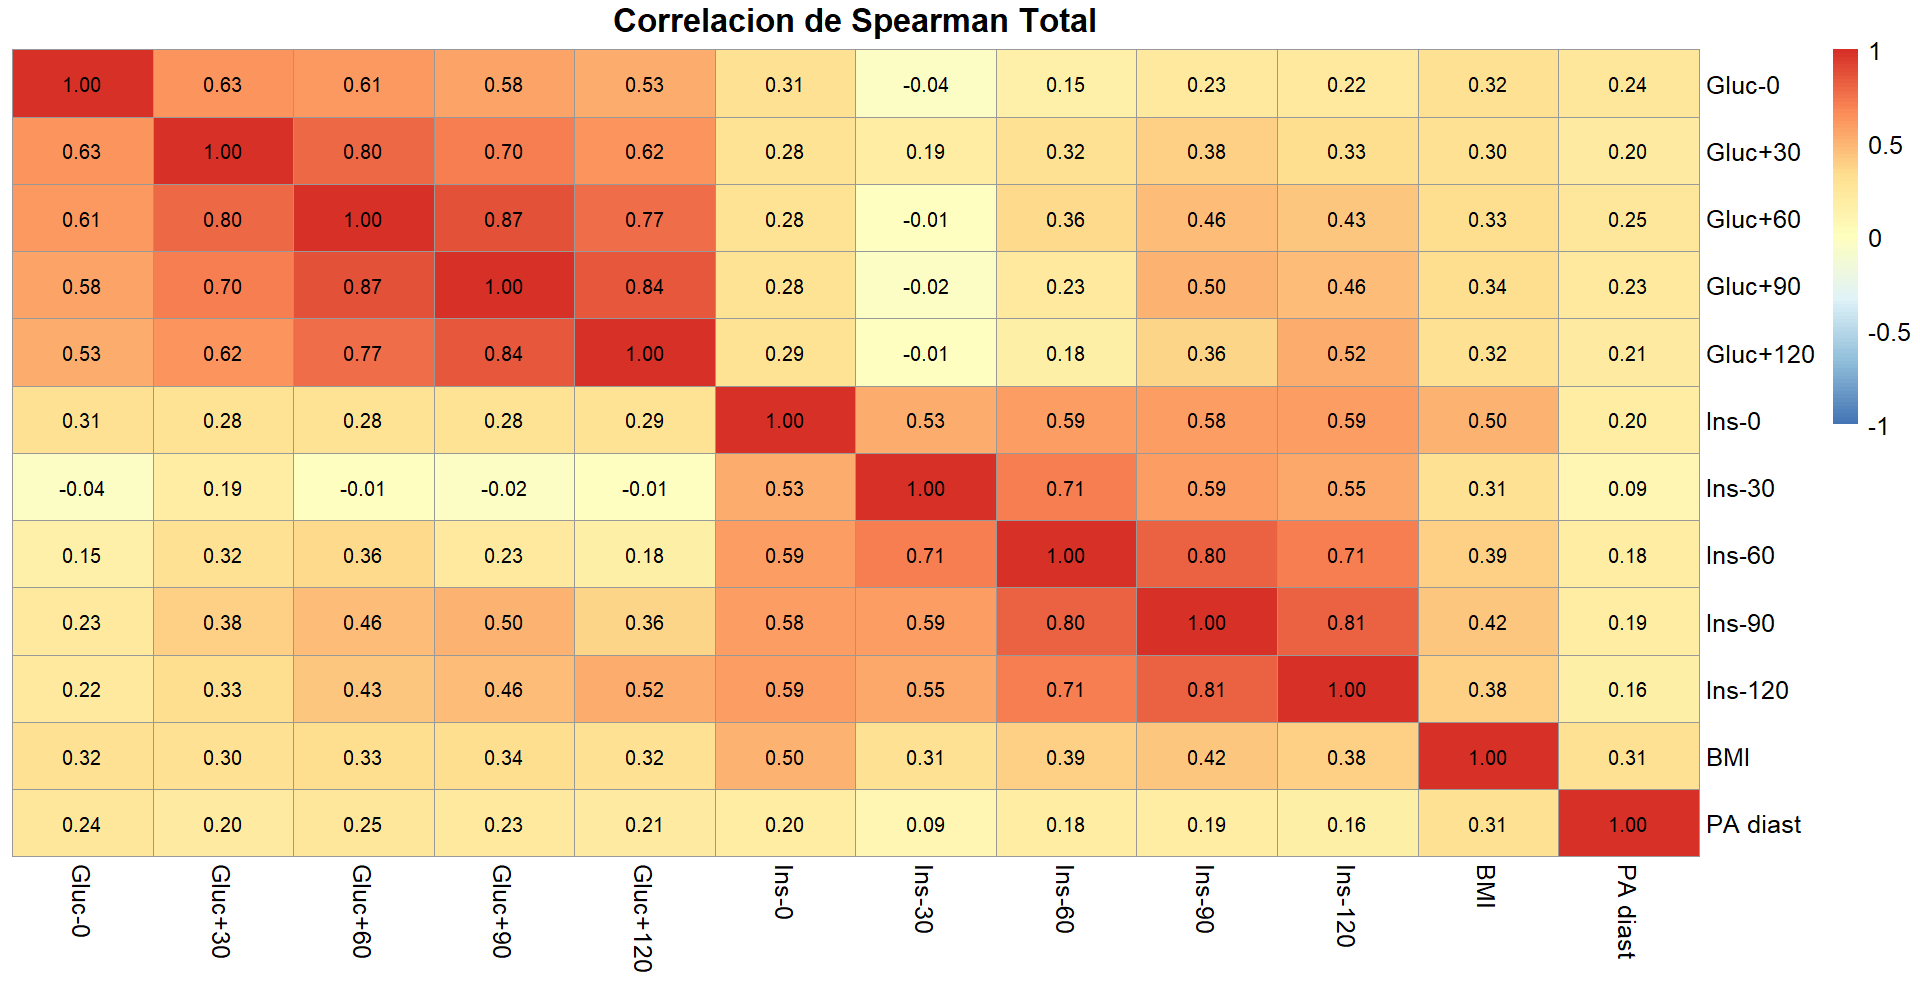
\includegraphics[width = 0.9 \textwidth]{Imagenes/corSperTotal.png}
    \caption{Heatmap de las covariables numéricas con la correlación de Spearman.}
    \label{fig:corSpe}
\end{figure}

El objetivo es utilizar las cópulas para modelar adecuadamente las interacciones entre la glucosa y la insulina, ya que estas interacciones son fundamentales para inferir el estado de las células beta del páncreas y proporcionar una alerta adecuada sobre la enfermedad. Al capturar la naturaleza compleja y no lineal de estas dependencias, el uso de cópulas permite una representación más precisa de las relaciones subyacentes, mejorando así la capacidad de detección temprana y el manejo de enfermedades como la diabetes.


\begin{figure}[H]
 \centering
  \subfloat[Mujeres]{
   \label{CorWolfMu}
    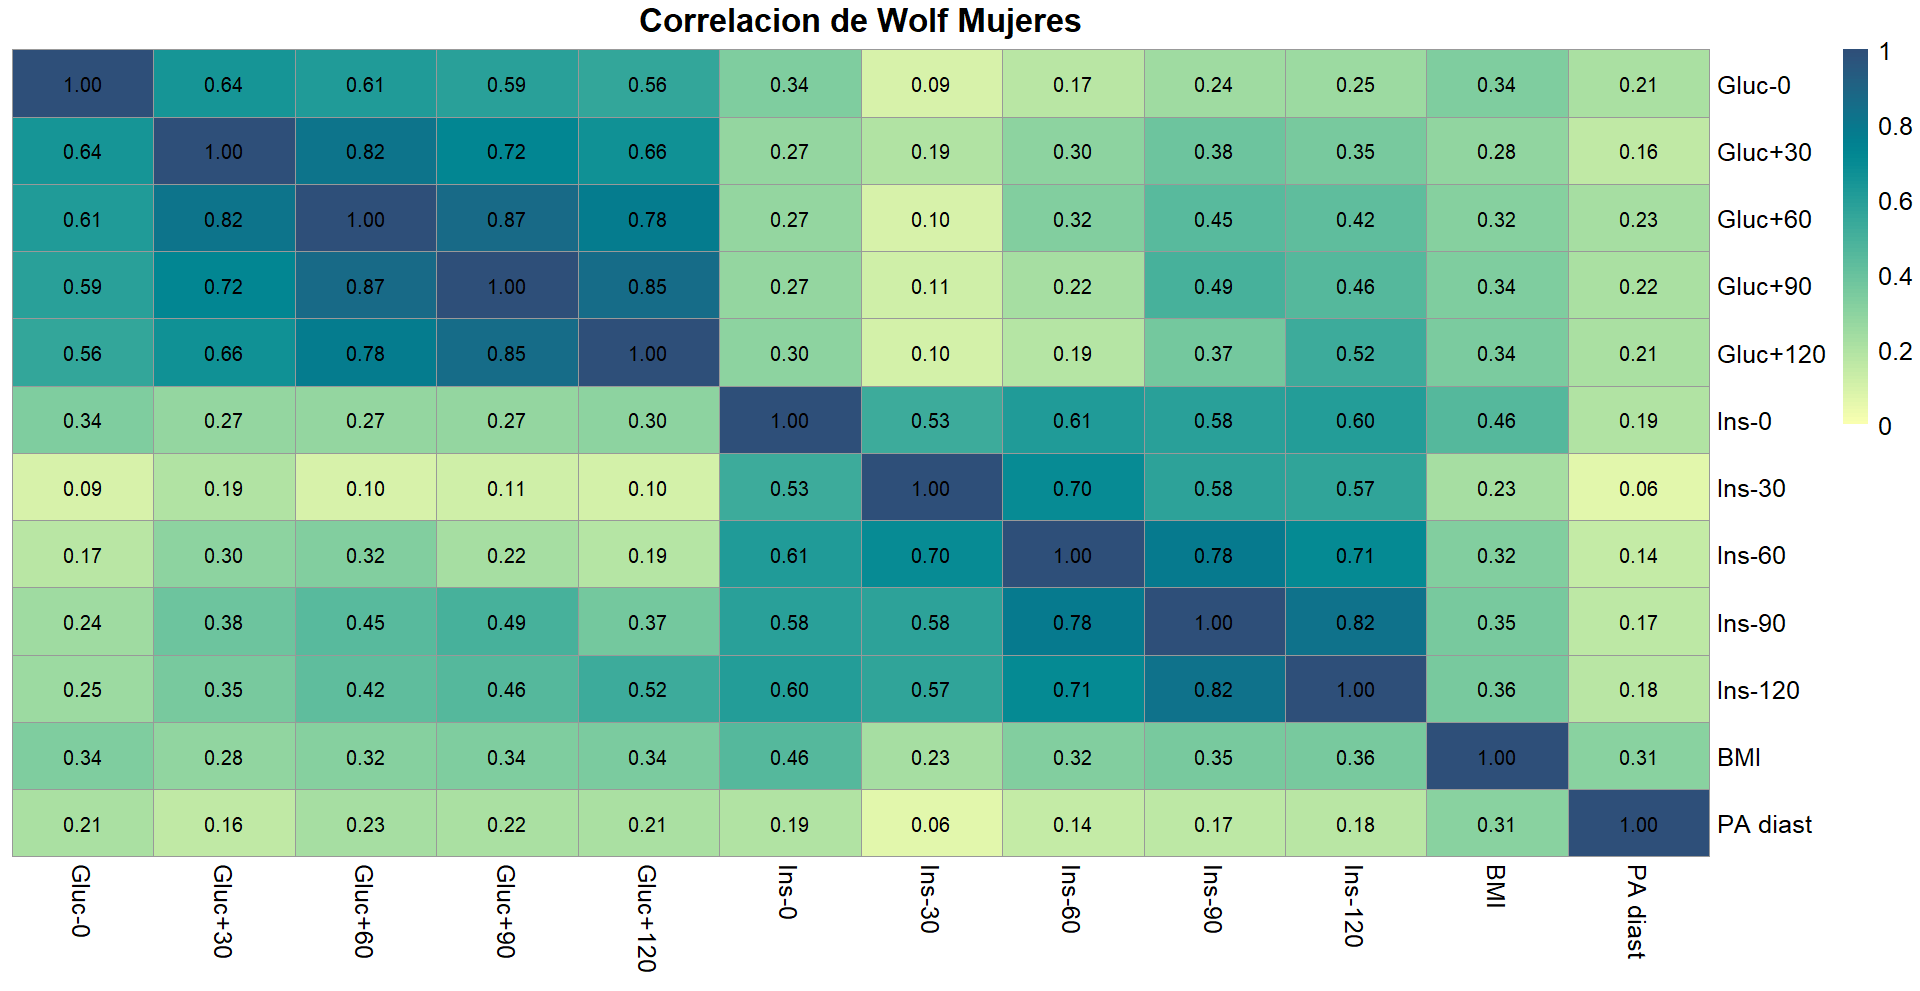
\includegraphics[width=0.48\textwidth]{Imagenes/corWolfMuj.png}}
  \subfloat[Hombres]{
   \label{CorWolfHom}
    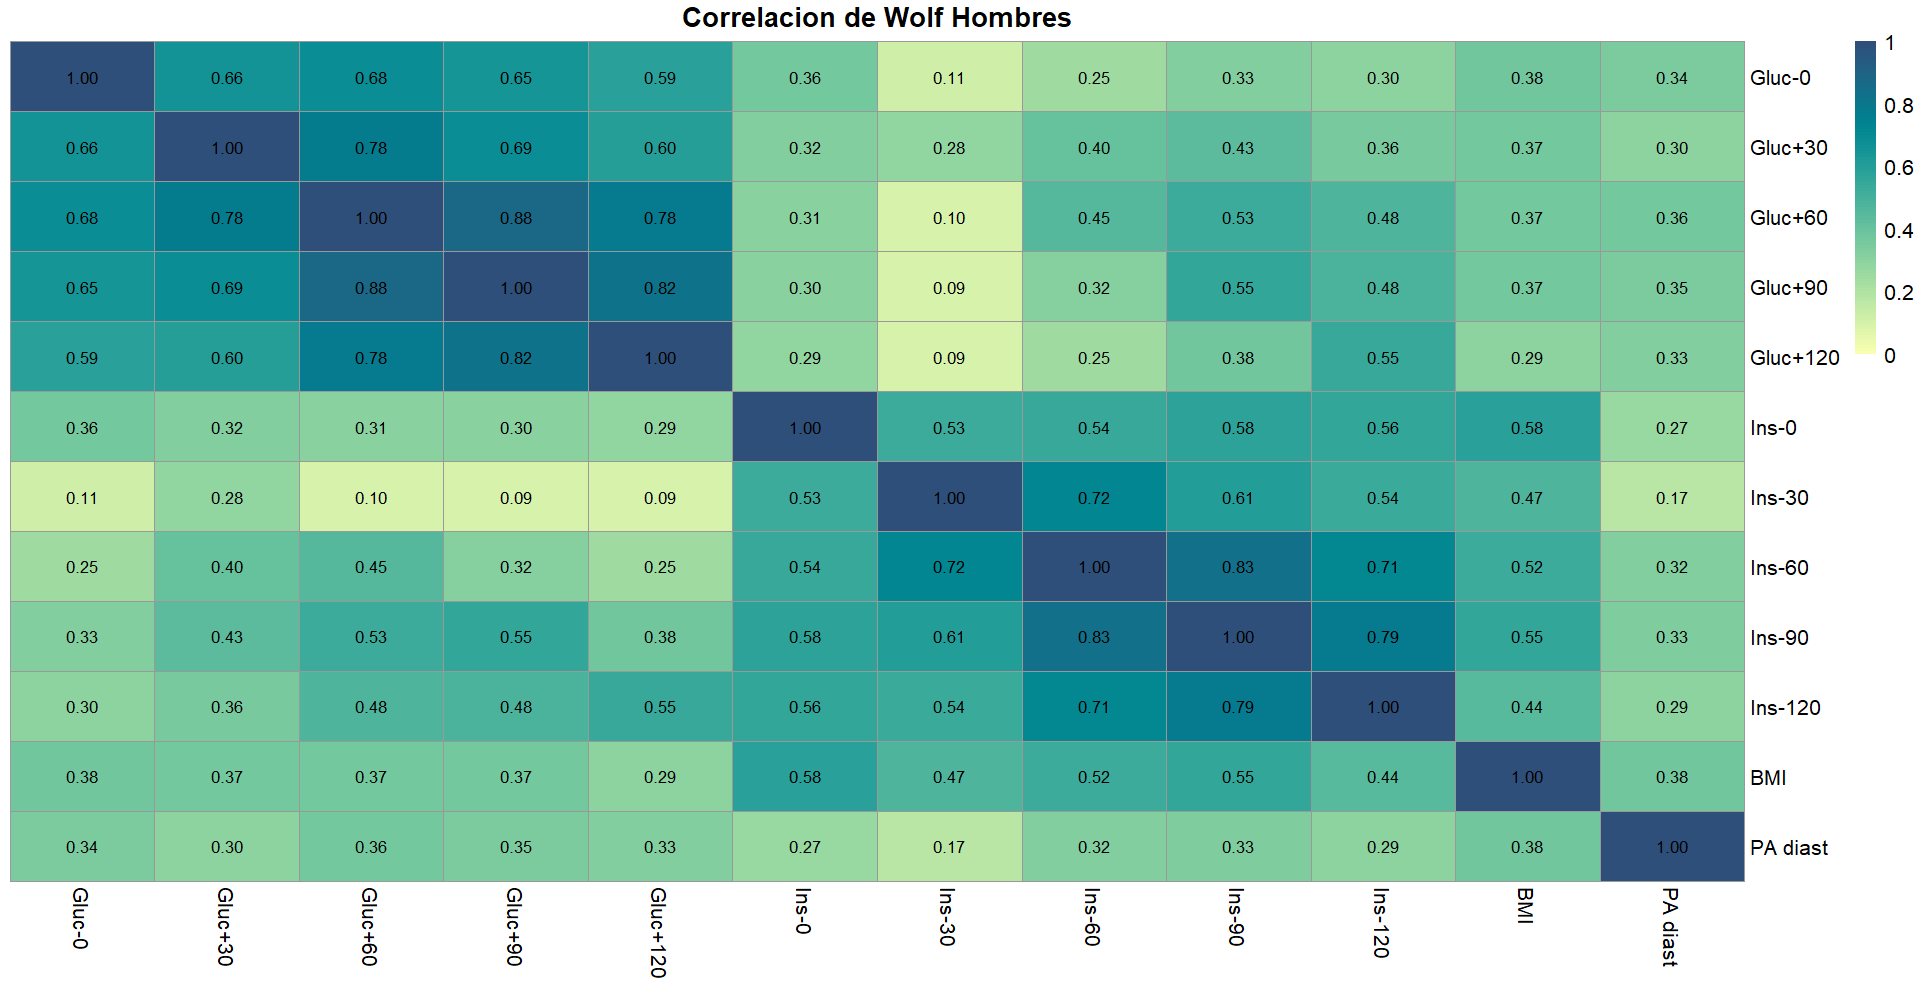
\includegraphics[width=0.48\textwidth]{Imagenes/corWolfHom.png}}
    \caption{Visualización de heatmaps por Género.}
    \label{fig:CorWolfGen}
\end{figure}

En la Figura \ref{fig:CorWolfGen}, se presentan los mapas de calor de la matriz de correlación de Wolf, desglosados por género. Sin embargo, no se aprecian diferencias significativas. Aunque algunas relaciones entre glucosa e insulina son más fuertes en mujeres que en hombres. Esto podría deberse al desbalance en la cantidad de datos disponibles, más que a una diferencia intrínseca relacionada con el género. Se espera que el modelo basado en cópulas sea capaz de discernir estas diferencias y proporcionar una interpretación más precisa de las dependencias entre las variables, tomando en cuenta tanto el posible desbalance de datos como las variaciones debidas al género.


%%%%%%%%%%%%%%%%%%%%%%%%%%%%%%%%%%%%%%%%%%%%%%%%%%%%%%%%5
%%%%%%%%%%%%%%%%%%%%%%%%%%%%%%%%%%%%%%%%%%%%%%%%%%%%%%%%%

 \subsection{Clasificación de Variables}\label{ClasificaVar}

\begin{table}[H]
    \centering
    \begin{tabular}{||c|c||}
    \hline\hline
    \textbf{Rango}                  & \textbf{Clasificación} \\ \hline\hline
    $ BMI < 25$            & Normal                 \\ \hline
    $25\leq BMI<30$                 & Sobrepeso              \\ \hline
    $ BMI > 35$               & Obesidad       \\ \hline\hline
\end{tabular}
\caption{Clasificación del grado de obesidad de acuerdo al IBM.}
\label{tab:clasBMI}
\end{table}

A partir de las variables que se tienen se pueden crear otras variables. A continuación, se describe las nuevas variables introducidas.  En función del índice de masa corporal, se introdujeron los grados de obesidad como la Dra. Monroy lo sugirió. En el Cuadro \ref{tab:clasBMI} se marca esta clasificación.
Como breve resumen, se clasificaron $375$ como normal, $594$ con sobrepeso, $397$ con obesidad $1$, $158$ con obesidad $2$ y $71$ con obesidad $3$. 
 


En base a las mediciones en el tiempo de las concentraciones de glucosa se puede hacer una clasificación. En el Cuadro \ref{tab:diagnostico} se puede distinguir estas clasificaciones, las cuales fueron hechas de acuerdo a otra sugerencia de la Dra. Monroy. Como resultado de esta división, se encuentran $82$ diabéticos, $567$ con prediabéticos y $916$ individuos en un estado normal.

\begin{table}[H]
\centering
\begin{tabular}{||c|c||}
\hline\hline
\textbf{Criterio}                       & \textbf{Diagnóstico} \\ \hline\hline
$G_0 \leq100$ y $G_{120} \leq 140$   & Normal               \\ \hline
$G_{0} > 100$ y $G_{0} < 126$  & Prediabetes          \\ \hline
$G_{120} \geq 140$ y $G_{120} < 200$ & Prediabetes          \\ \hline
$G_0 \geq 126$                     & Diabetes             \\ \hline
$G_{120} \geq 200$                  & Diabetes             \\ \hline
En otro caso                            & Incierto              \\ \hline\hline
\end{tabular}
\caption{Diagnóstico de acuerdo a la curva de Glucosa.}
\label{tab:diagnostico}
\end{table}

Con el objetivo de visualizar el procesamiento de glucosa e insulina de acuerdo al índice de masa corporal, en la Figura \ref{fig:CurvasGluIBM} se muestran las curvas de glucosa clasificadas según la categoría de índice de masa corporal. Algunos aspectos destacables son los siguientes: 

\begin{figure}[H]
    \centering
    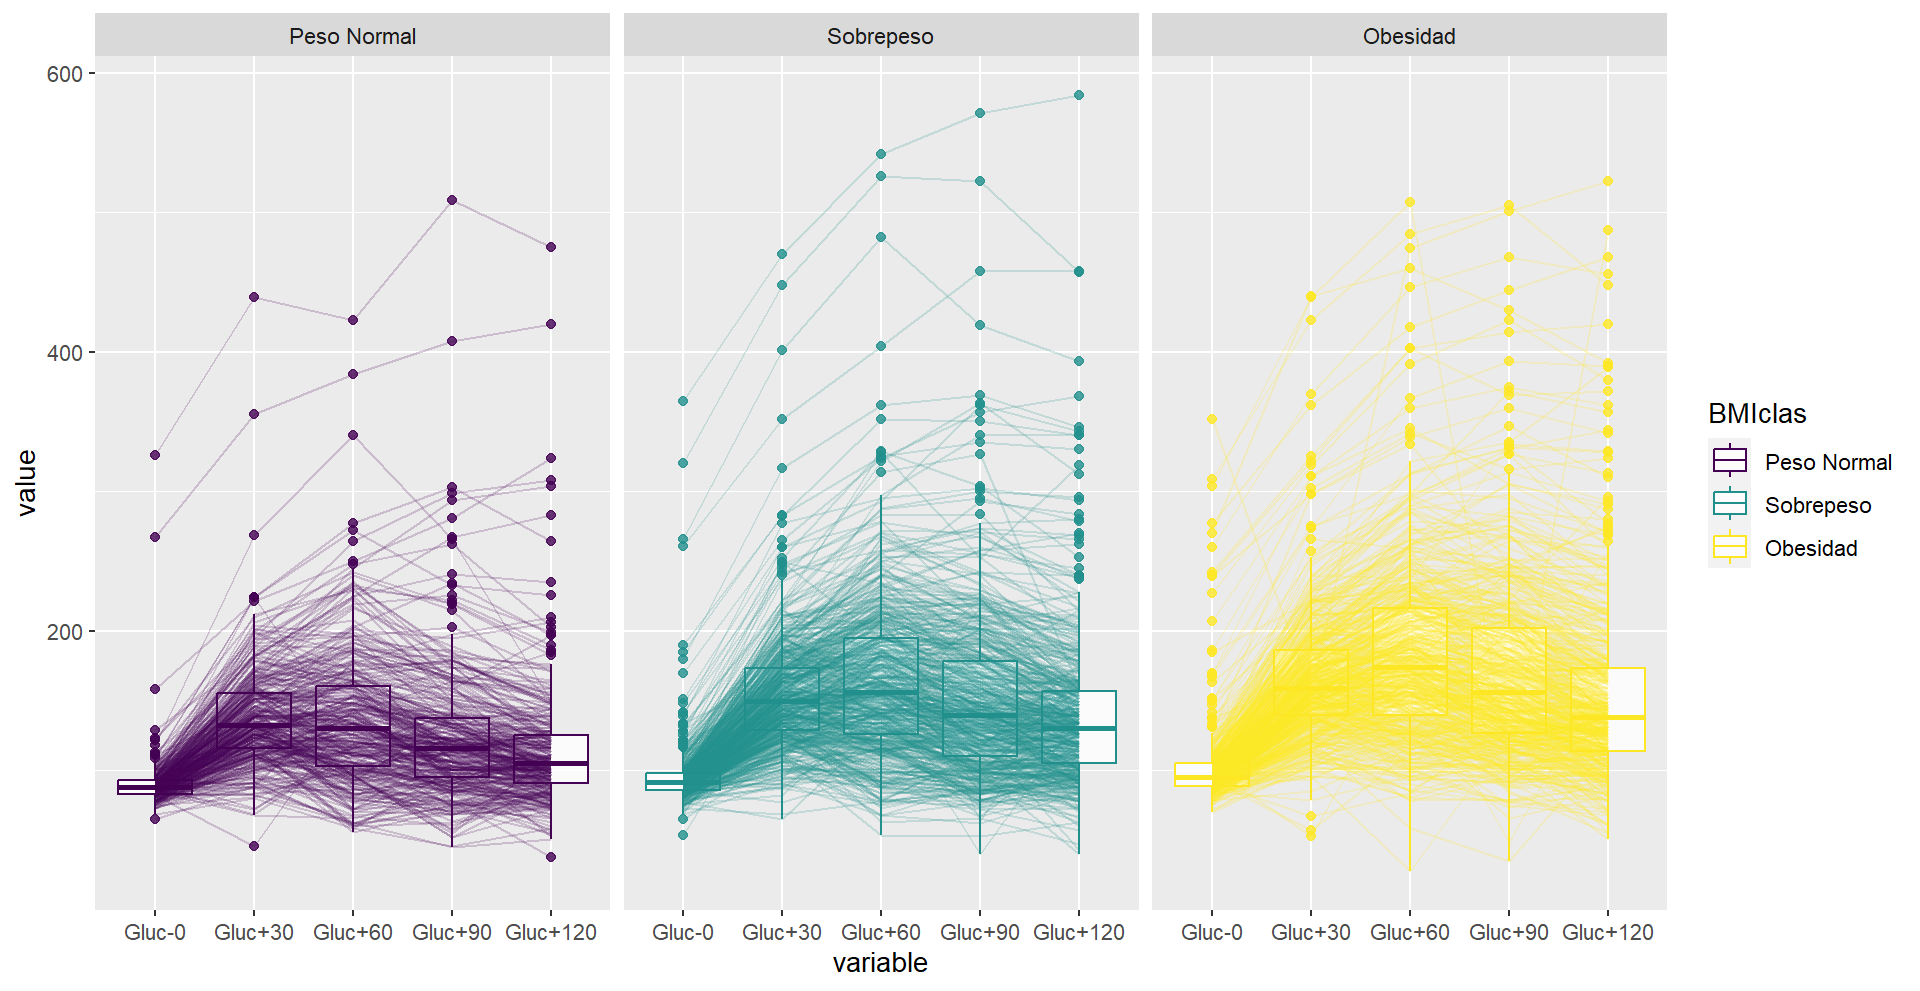
\includegraphics[width = 0.98 \textwidth]{Imagenes/gluCurvasBMI.png}
    \caption{Curvas de glucosa acuerdo al índice de masa corporal.}
    \label{fig:CurvasGluIBM}
\end{figure}

\begin{itemize}
    \item Los pacientes con peso normal mayoritariamente presentan curvas de glucosa dentro de los rangos esperados, como se observa en los boxplots a los tiempos $0$ y $120$, donde los valores son más bajos en comparación con pacientes con sobrepeso u obesidad. Sin embargo, es importante destacar que tener un peso normal no garantiza estar libre de riesgos, ya que también se pueden observar curvas con niveles elevados de glucosa.

    \item Los pacientes con sobrepeso muestran mayor variabilidad, con rangos más altos, especialmente a los minutos $90$ y $120$. Esto se puede observar en los boxplots correspondientes a eso minutos. En este grupo es donde se observa el paciente con la curva de glucosa más alta, lo cual podría indicar estrés en las células beta del páncreas.

    \item Los individuos con obesidad presentan curvas con rangos más altos en los minutos $60$, $90$ y $120$, como se refleja en sus respectivos boxplots.  Sin embargo, también se observa que hay más individuos dentro de este grupo que muestran curvas con niveles muy elevados de glucosa pero también se encuentran individuos con curvas en rangos normales, lo cual indica que la obesidad es un factor influyente pero no determinante.
\end{itemize}

Como conclusión de estas observaciones, se espera que las cópulas puedan capturar esta relación, ya que el índice de masa corporal influye en el diagnóstico de la diabetes, aunque no de manera determinante. Si bien los individuos con sobrepeso u obesidad tienden a mostrar niveles más altos de glucosa e insulina, también se observa una considerable variabilidad dentro de estos grupos. Esto sugiere que la obesidad es un factor importante pero no único en la predisposición a la diabetes.


\begin{figure}[H]
    \centering
    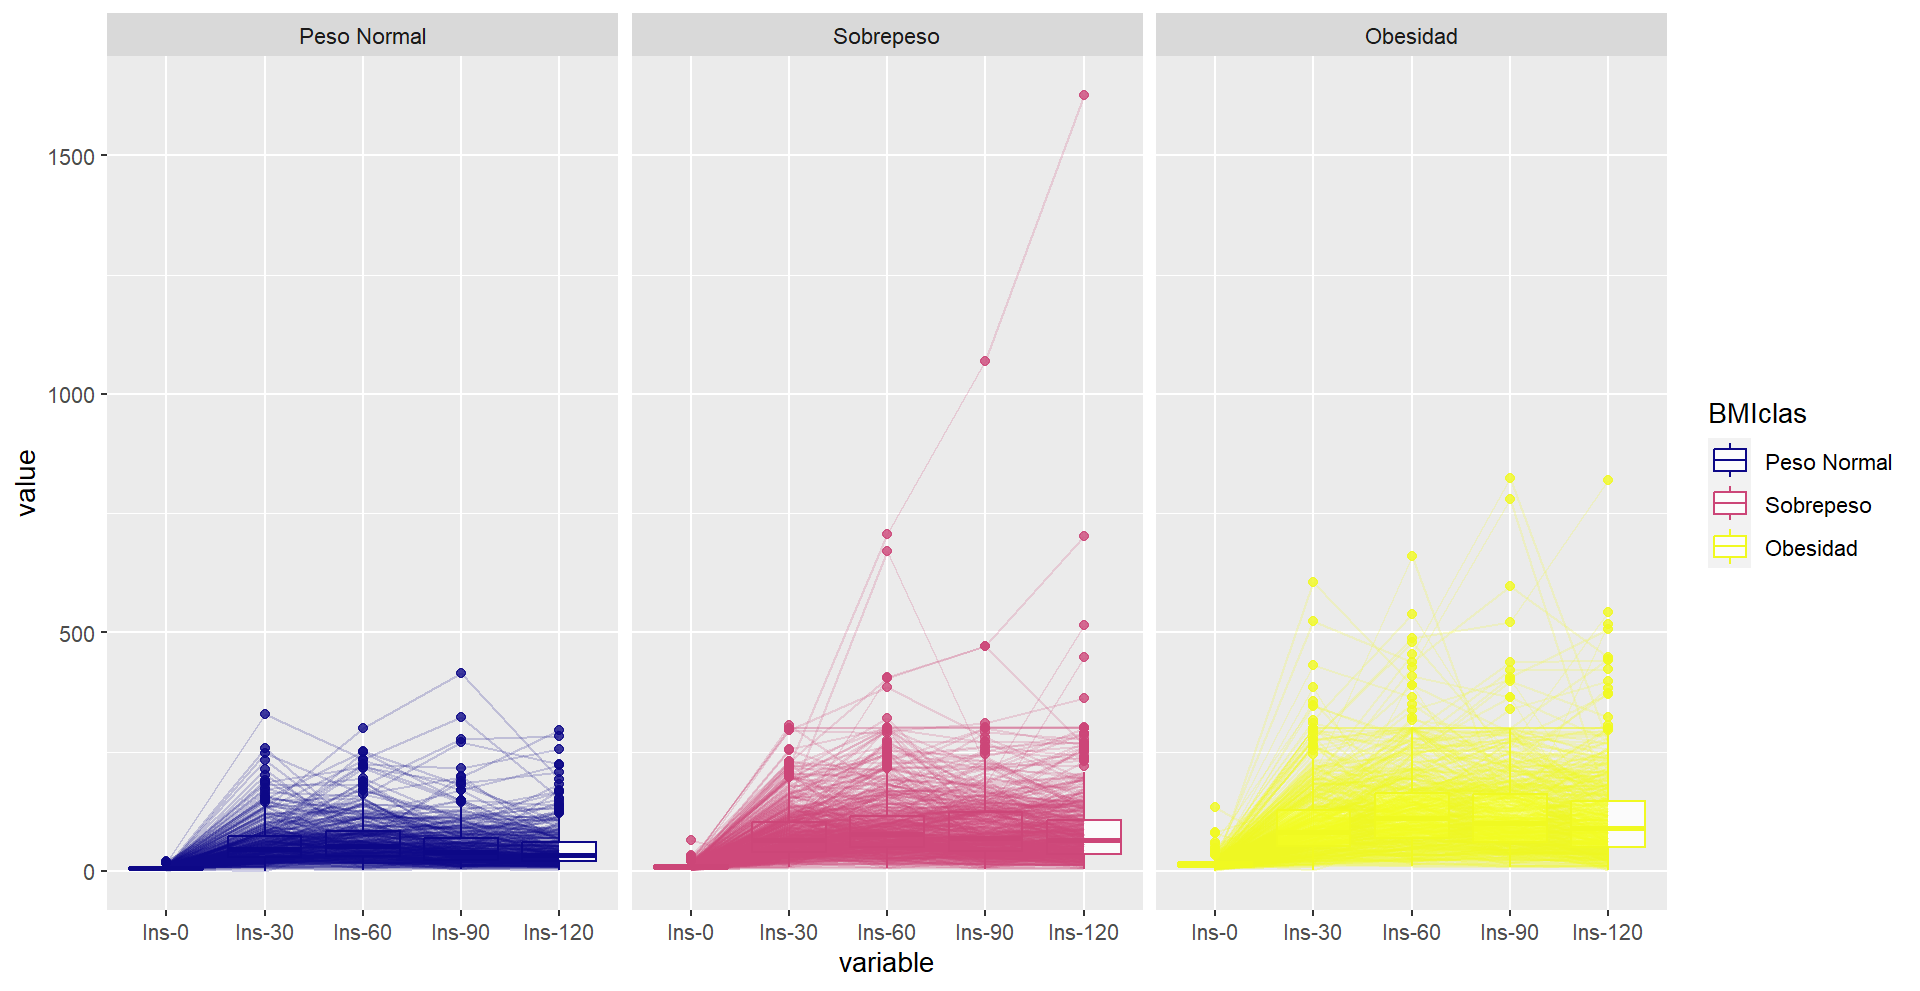
\includegraphics[width = 0.9 \textwidth]{Imagenes/insCurvasBMI.png}
    \caption{Curvas de insulina de acuerdo al índice de masa corporal.}
    \label{fig:CurvasInsIBM}
\end{figure}

Para continuar con este análisis por índice de masa corporal, en la Figura \ref{fig:CurvasInsIBM} se muestran las curvas de respuesta de la insulina. Los elementos destacables son:

\begin{itemize}
    \item  Las curvas correspondientes a pacientes con peso normal muestran un patrón generalmente cóncavo. Sin embargo, también se pueden observar casos donde la curva no sigue este patrón cóncavo tan pronunciado, sino que inicialmente es creciente y luego apenas decrece en los últimos minutos, lo cual podría indicar un inicio de falló en la efectividad de la insulina.

    \item Los pacientes con sobrepeso presentan curvas muy variadas. Algunos muestran la característica forma cóncavo, que es indicativa de una respuesta normal de la insulina. Sin embargo, también se observan curvas que parecen ser simplemente crecientes, lo cual sugiere una clara disfunción de las células beta del páncreas. Este patrón indica un inicio de fallo en la efectividad de la insulina, siendo un hallazgo preocupante en pacientes con sobrepeso.

    \item Los pacientes con obesidad presentan curvas que sugieren resistencia a la insulina en diferentes grados. Algunas curvas muestran un descenso en los últimos instantes, lo cual indica que la resistencia a la insulina podría ser reversible en cierta medida. Sin embargo, también se observan curvas donde la producción de insulina es prácticamente nula. Esto sugiere un claro agotamiento de las células beta del páncreas, lo cual es preocupante y podría indicar un deterioro avanzado en la capacidad del cuerpo para regular los niveles de glucosa.
    \end{itemize}

Como se pudo observar anteriormente, la relación entre la glucosa y la insulina no es trivial de modelar. En la siguiente sección, se hará más énfasis en esta relación y en los momentos cruciales para identificar y alertar antes de que esta enfermedad sea irreversible.

%%%%%%%%%%%%%%%%%%%%%%%%%%%%%%%%%%%%%%%%%%%%%%%%%%%%%%%%%%%%
%%%%%%%%%%%%% Resultados de Boxplot Funcioles %%%%%%%%%%%%%%
%%%%%%%%%%%%%%%%%%%%%%%%%%%%%%%%%%%%%%%%%%%%%%%%%%%%%%%%%%%%

\section{Resultados de Boxplot Funcionales}

Según el artículo `\textit{Gender differences in glucose homeostasis and diabete}' \cite{GenderDifferences2018}, existen diferencias notables en el proceso de homeostasis de la glucosa entre hombres y mujeres que pueden ser relevantes durante el modelado. Esto adquiere importancia porque el propósito es desarrollar dos modelos distintos para predecir la resistencia a la insulina. Por ejemplo, se destaca que las mujeres muestran niveles más bajos de glucosa plasmática en ayunas y niveles más altos de glucosa plasmática a las 2 horas en comparación con los hombres.

\subsection{Construcción de un Boxplot Funcional}

Antes del comenzar el análisis gráfico, se presentará una breve descripción de la construcción de los boxplots funcionales para mejorar la interpretación de la gráfica para algo más detallada se sugiera consultar el artículo `\textit{Functional Boxplots}' \cite{boxplotFun}. La construcción de los boxplots funcionales sigue un proceso similar al de los boxplots clásicos, pero utiliza una medida de profundidad como las descritas en el Capítulo \ref{RegCuanDatosFun}:

\begin{figure}[H]
    \centering
    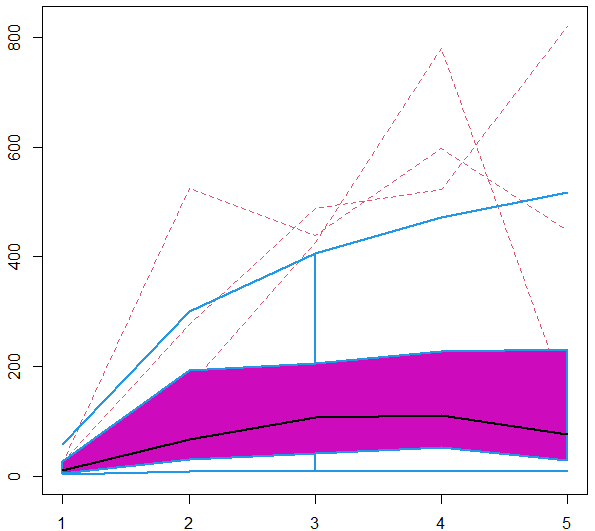
\includegraphics[width=0.5\linewidth]{Imagenes/partes.png}
    \caption{Parte de un Boxplot Funcional.}
    \label{fig:bfpartes}
\end{figure}

\begin{itemize}
    \item \textbf{Curva más profunda}. Se identifica la curva central o más profunda de las funciones empleando la medida de profundidad, que es la región donde se encuentra la mitad central de las curvas de datos, esta se muestra en negro en la Figura \ref{fig:bfpartes}. La curva mediana es una estadística robusta para medir la centralidad de las funciones.

    \item \textbf{El envolvente o caja}. Esta región es análoga al rango intercuartílico en un boxplot tradicional, y proporciona una indicación útil de la dispersión del $50\%$ central de las curvas. Esta esta definida por

    \begin{equation}
        C_{0.5} = \left\{(t, x(t)): \min _{r=1, \ldots,\lceil n / 2\rceil} x_{[r]}(t) \leq x(t) \leq \max _{r=1, \ldots,\lceil n / 2\rceil} x_{[r]}(t)\right\},
    \end{equation}

    donde $n$ es total de datos, $ \left \lceil \frac{n}{2}\right \rceil$ es el entero no más grande que $n/2$ y a $C_{0.5}$ se le llama el envolvente del $50 \%$. Esta se muestra en lila en la Figura \ref{fig:bfpartes}.
    
    \item \textbf{Bigotes}. Estos son líneas verticales que se extienden desde la caja y representan el máximo envolvente del conjunto de datos, excepto los outliers. Se construyen extendiendo el criterio de $1.5$ veces el rango intercuartílico de un boxplot tradicional. Para ello, se infla el envolvente de $50\%$ multiplicando su rango por $1.5$. En la Figura \ref{fig:bfpartes}, corresponden a las lineas azules.

    \item \textbf{Outliers}. Cualquier curva que se encuentre por fuera de los bigotes es marcada como un outlier. Estas curvas están marcadas con lineas rojas punteadas en la Figura \ref{fig:bfpartes}.
\end{itemize}
%%%%%%%%%%%%%%%%%%%%%%%%%%%%%%%%%%%%%%%%%%%%%%%%%%%%%%%%%%
%%%%%%% Boxplot's Funcionales de Glucosa e Insulina %%%%%% 
%%%%%%%%%%%%%%%%%%%%%%%%%%%%%%%%%%%%%%%%%%%%%%%%%%%%%%%%%%

\subsection{Boxplot's funcionales para la Glucosa e Insulina}

A continuación, se llevará a cabo un análisis exploratorio para identificar elementos relevantes, como las diferencias en las formas o rangos de las curvas de glucosa e insulina entre los grupos de hombres y mujeres, así como los grupos definidos por las clasificaciones del prediagnóstico sugerido.



\begin{figure}[H]
 \centering
  \subfloat[Boxplot Funcional de glucosa]{
   \label{bfGluTotal}
    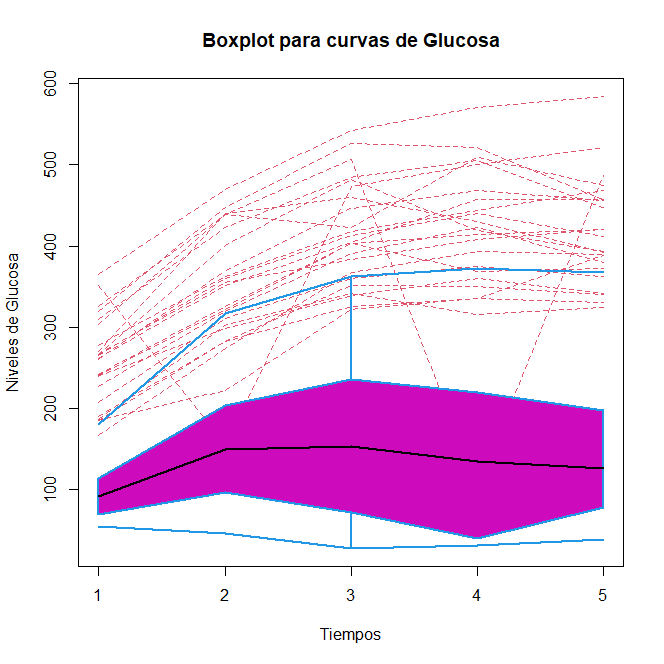
\includegraphics[width=0.47\textwidth]{img/bfTotalGlu.png}}
  \subfloat[Curvas de glucosa]{
   \label{dispGluTotal}
    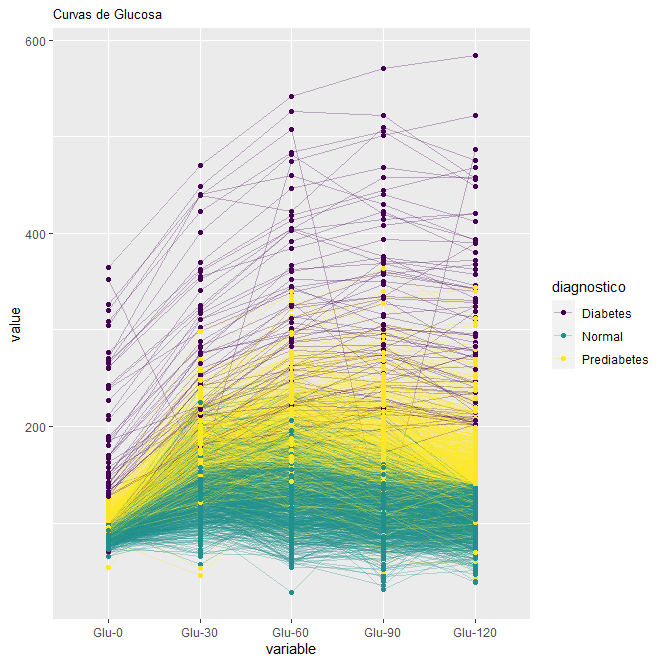
\includegraphics[width=0.47\textwidth]{img/disperGlu.png}}
    \caption{Gráficos de exploración de las curvas de glucosa.}
    \label{fig:glucosa}
\end{figure}


En la figura \ref{bfGluTotal} se presenta un boxplot funcional de las curvas de glucosa. El comportamiento de la curva mediana alcanza su punto máximo durante los primeros $60$ minutos y luego comienza a descender. Se observa que la mayoría de los datos atípicos corresponden al grupo de diabéticos, indicado en morado en la Figura \ref{dispGluTotal}. Además, se identifican algunos datos cuyas curvas parecen tener un patrón de subida, bajada y nueva subida, lo cual sugiere la posibilidad de errores de medición o que sugieren un error inherente. Otro aspecto destacable es la similitud entre las curvas correspondientes al tercer y primer cuartil, lo que sugiere una tendencia consistente en el procesamiento de la glucosa en sangre dentro de estos rangos.


\begin{figure}[H]
 \centering
  \subfloat[Boxplot Funcional de insulina]{
   \label{bfInsTotal}
    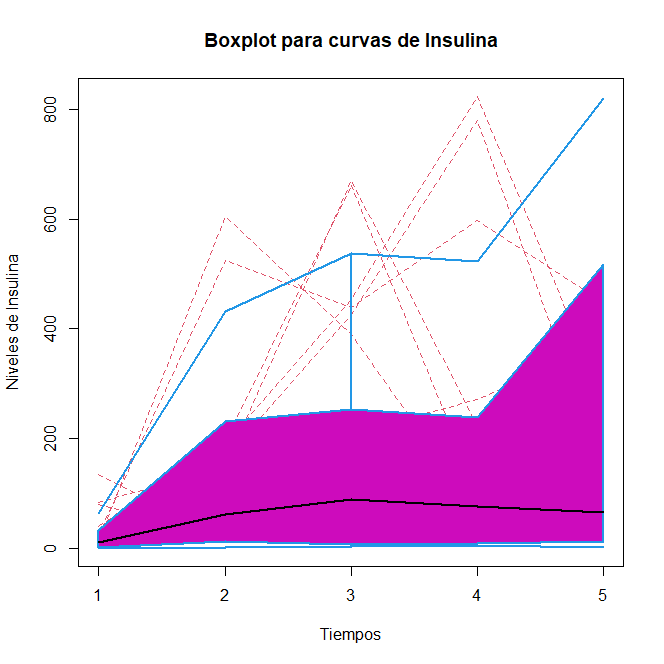
\includegraphics[width=0.47\textwidth]{img/bfTotalIns.png}}
  \subfloat[Curvas de insulina]{
   \label{dispInsTotal}
    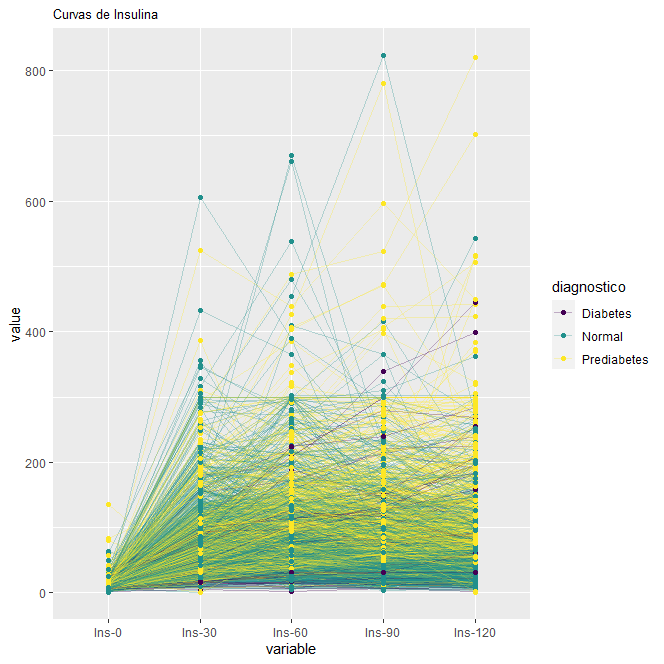
\includegraphics[width=0.47\textwidth]{img/dispeIns.png}}
    \caption{Gráficos de exploración de las curvas de insulina.}
    \label{fig:insulina}
\end{figure}

La falta de una separación clara en las curvas de insulina de la Figura \ref{dispInsTotal}, puede deberse a varios factores. Durante la etapa en la que el paciente tiene una producción normal de insulina, es esperable que esta aumente inicialmente y luego disminuya. En la etapa de prediabetes, la producción de insulina tiende a elevarse a niveles más altos de lo habitual para posteriormente descender, y en los casos más avanzados, los niveles de insulina pueden aumentar a lo largo de toda la curva. Los pacientes catalogados como diabéticos suelen tener una producción insuficiente de insulina, lo que se refleja en niveles bajos de insulina durante la mayor parte del tiempo. Esta variabilidad en la producción de insulina entre los diferentes estados de salud puede contribuir a la falta de separación clara en las curvas de insulina observadas.


La dificultad para visualizar claramente los grupos puede atribuirse al hecho de que los niveles de insulina tanto en pacientes normales como en diabéticos tienden a ser bajos, siendo aún más bajos en los pacientes diabéticos. Además, es posible observar algunos pacientes cuyas curvas de glucosa se catalogan como normales, pero cuyas curvas de insulina muestran niveles más altos de lo habitual. Un objetivo de la tesis es poder mejorar esta disociación entre los niveles de glucosa e insulina.


El boxplot funcional parece proporcionar indicios de las tres clasificaciones. La curva del tercer cuartil muestra rangos muy altos y una forma creciente, lo que sugiere un patrón prediabético. Por otro lado, la curva del primer cuartil, debido al rango en el que se encuentra, podría corresponder a la de un paciente diabético. Finalmente, la curva mediana muestra un rango relativamente bajo y una forma ascendente seguida de una disminución, lo que indica un perfil normal en un paciente.

%%%%%%%%%%%%%%%%%%%%%%%%%%%%%%%%%%%%%%%%%%%%%%%%%%
%%% A N A L I S I S  P O R   C O N D I C I O N %%%
%%%%%%%%%%%%%%%%%%%%%%%%%%%%%%%%%%%%%%%%%%%%%%%%%%
\subsection{Boxplots funcionales por Prediagnóstico}

Para comprender la estructura de los datos funcionales, se realizará una visualización basada en el prediagnóstico. Esto permitirá entender mejor la relación entre la glucosa y la insulina en cada etapa.

En la Figura \ref{bfGluNormal} se muestra el boxplot funcional de glucosa de los pacientes cuyo prediagnóstico es normal. Este conjunto de datos no presenta datos atípicos. La curva más profunda aumenta hasta el minuto 30, alcanzando niveles de alrededor de $180$ $mg/dl$, para luego descender suavemente. En general, las curvas correspondientes al primer y tercer cuartil tienen una forma cóncava similar. Sin embargo, la curva del tercer cuartil mantiene niveles altos hasta el minuto 90, lo que podría indicar principios de estrés en las células beta. Adicionalmente, el ancho de la banda no parece ser muy variable ni demasiado amplio, lo cual sugiere una estabilidad en la varianza de las curvas.

El boxplot funcional de insulina de los pacientes con prediagnóstico normal que se expone en la Figura \ref{bfInsNormal}, muestra varios datos atípicos. Estos datos presentan rangos muy altos en ciertos momentos, tomando la forma de una curva que crece rápidamente, alcanzando su pico entre los minutos 30 y 90, para luego descender. Este comportamiento evidencia los altos niveles de producción de insulina necesarios para regular adecuadamente la glucosa en sangre.

\begin{figure}[H]
 \centering
  \subfloat[Glucosa]{
   \label{bfGluNormal}
    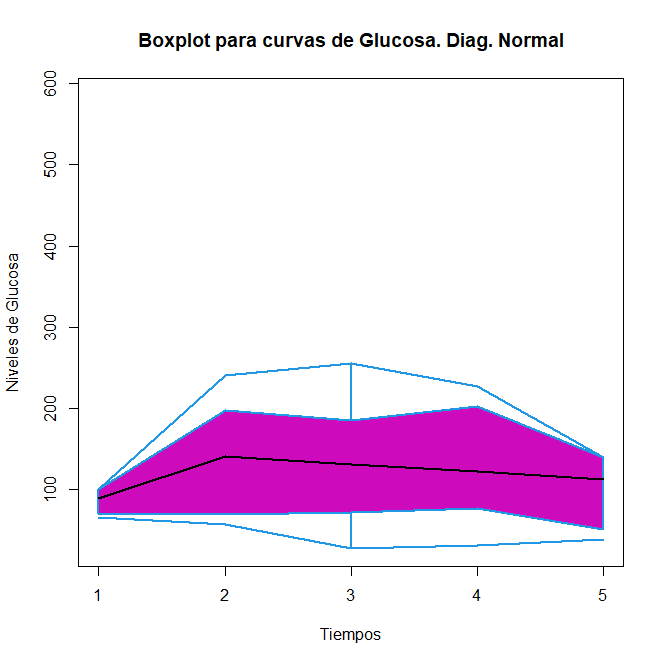
\includegraphics[width=0.45\textwidth]{img/bfgluNormal.png}}
  \subfloat[Insulina]{
   \label{bfInsNormal}
    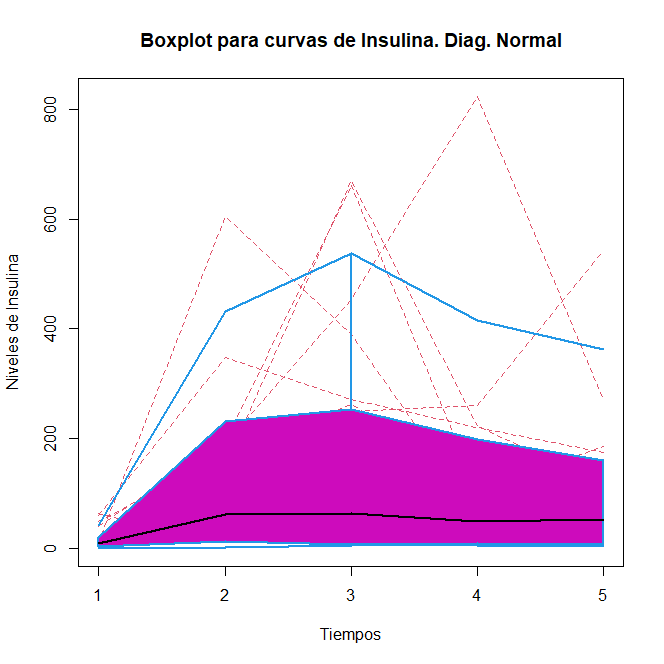
\includegraphics[width=0.45\textwidth]{img/bfInsNormal.png}}
    \caption{Boxplot funcional para las curvas de glucosa e insulina para personas con prediagnóstico normal.}
    \label{fig:bfNormal}
\end{figure}

La curva más profunda muestra un crecimiento muy suave desde el minuto 0 hasta el 30, para luego mantenerse con ligeras variaciones durante los próximos 90 minutos. Las curvas correspondientes al primer y tercer cuartil son muy distintas. El espacio entre la curva media y la del tercer cuartil es muy grande, indicando una gran variedad de rangos, aunque la forma se mantiene similar. Esto se puede interpretar como el inicio de una disminución en la eficiencia de la insulina sobre la glucosa. En cuanto a la curva del primer cuartil, tiene una forma y rango similar a la más profunda, lo que indica poca variabilidad en este conjunto. Aunque la forma de las curvas se mantiene consistente. Esto sugiere que, aunque hay diferencias en la cantidad de insulina producida, la respuesta general del cuerpo a la glucosa es bastante uniforme en este grupo.

\begin{figure}[H]
 \centering
  \subfloat[Glucosa]{
   \label{bfGluPre}
    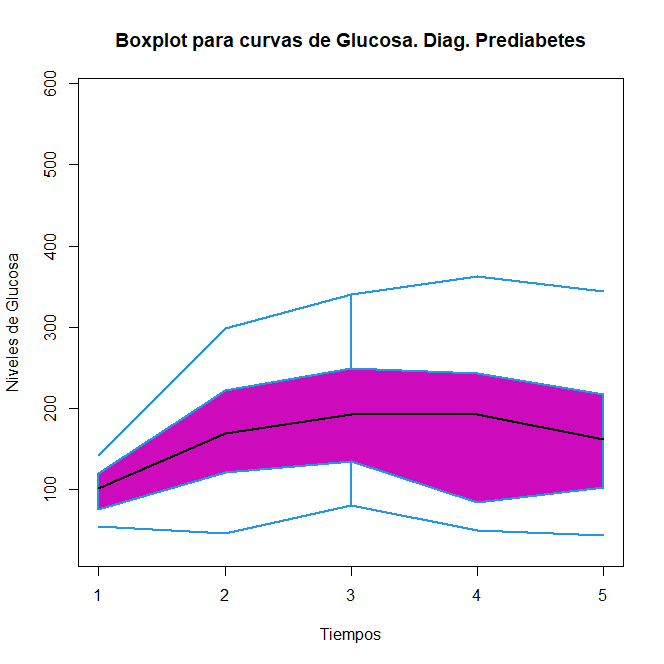
\includegraphics[width=0.48\textwidth]{img/bfgluPredia.png}}
  \subfloat[Insulina]{
   \label{bfInsPre}
    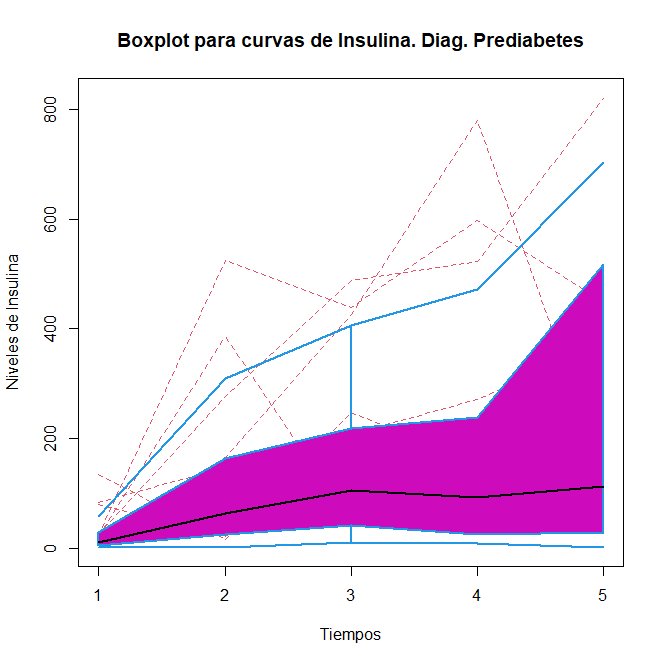
\includegraphics[width=0.48\textwidth]{img/bfInsPredia.png}}
    \caption{Boxplot funcional para las curvas de glucosa e insulina para personas con prediagnóstico prediabetes.}
    \label{fig:bfPrediabetes}
\end{figure}

La Figura \ref{bfGluPre} muestra el boxplot funcional de las curvas de glucosa para pacientes con prediagnóstico de prediabetes. Uno de los aspectos más destacables es el aumento en el rango de estas curvas en comparación con las de la categoría de diagnóstico normal. Por otra parte, la curva media aumenta suavemente hasta el minuto 90, para luego disminuir ligeramente en el minuto 120. Este comportamiento es similar para las curvas correspondientes al primer y tercer cuartil. Además, las distancias de estas curvas a la curva más profunda parecen ser similares, lo cual indica una varianza similar.

El boxplot de las curvas de insulina se puede ver en la Figura \ref{bfInsPre}. Se pueden apreciar datos atípicos, tanto en forma como en rango. Estos datos alcanzan niveles cercanos a 500 unidades, lo cual indica una sobreproducción de insulina y sugiere una posible falla de las células beta en un periodo de tiempo corto debido a nivel tan alto de hiperglucemia.

La curva más profunda muestra un crecimiento muy suave desde el minuto 0 hasta el 60, para luego mantenerse con ligeras variaciones durante los siguientes 60 minutos. Adicionalmente, las curvas correspondientes al primer y tercer cuartil son muy distintas. La curva del tercer cuartil es creciente en todo el dominio, lo cual indica una sobreproducción de insulina. Por otra parte, el espacio entre la curva media y la del tercer cuartil es muy grande, lo que indica una gran variedad en el rango y la forma de las curvas dentro de este subconjunto. Finalmente, la curva del primer cuartil parece tener una buena forma, ya que se encuentra muy pegada a la curva media. Así, el análisis del boxplot funcional de insulina revela una considerable variabilidad en la respuesta insulínica de los pacientes con prediagnóstico Prediabética. 


\begin{figure}[H]
 \centering
  \subfloat[Glucosa]{
   \label{bfGluDia}
    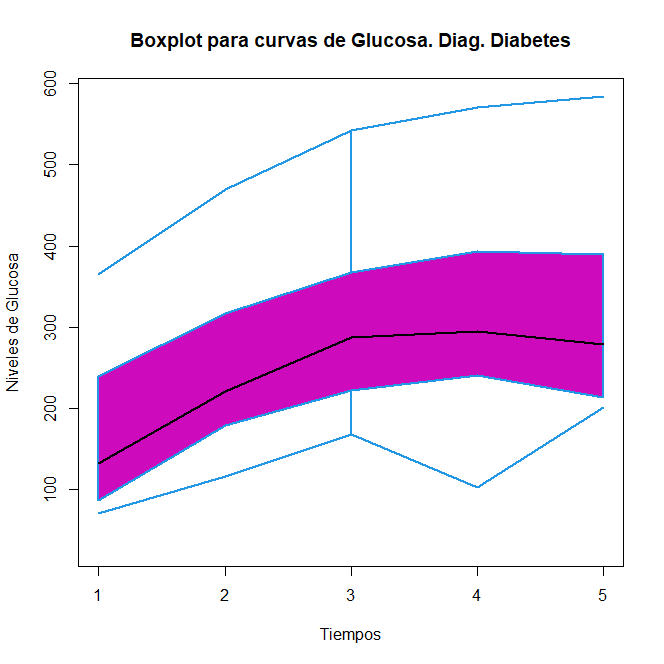
\includegraphics[width=0.48\textwidth]{Imagenes/fbGluDiabetes.png}}
  \subfloat[Insulina]{
   \label{bfInsDia}
    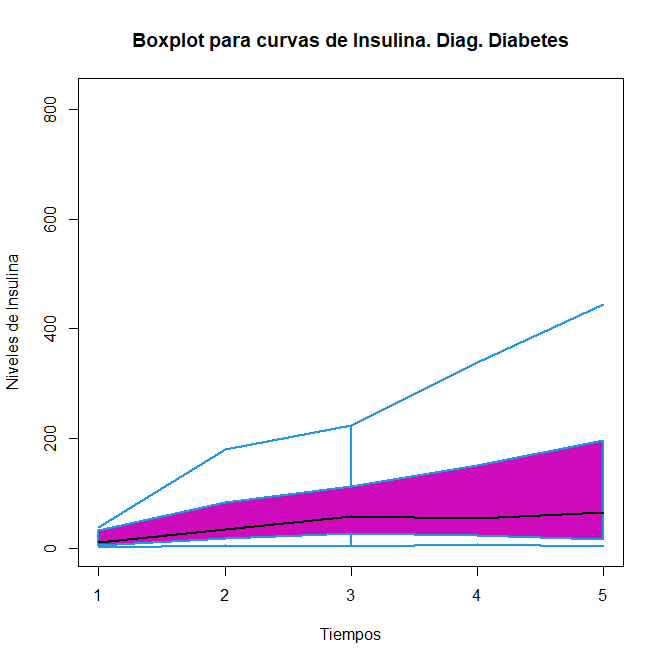
\includegraphics[width=0.48\textwidth]{img/bfInsDiabetes.png}}
    \caption{Boxplot funcional para las curvas de glucosa e insulina para personas con prediagnóstico diabético.}
    \label{fig:bfDiabetes}
\end{figure}

En la Figura \ref{bfGluDia}, se muestra el boxplot funcional de las curvas de glucosa de los pacientes con prediagnóstico de diabetes. Se observa que estas curvas abarcan un rango mucho mayor que las de las dos categorías anteriores, llegando incluso a valores cercanos a $600$. Además, la curva más profunda presenta un crecimiento más rápido que las otras dos y alcanza su punto máximo a los $90$ minutos, para luego disminuir ligeramente en los últimos $30$ minutos. Este comportamiento sugiere una respuesta casi nula de la insulina producida o de lo contrario la poca producción de insulina. 

Además, la separación entre las curvas relacionadas con el primer y tercer cuartil con respecto a la curva más profunda es mayor que en los casos anteriores, lo que indica una mayor varianza en los datos, aunque conservan la misma forma que la curva más profunda. Es importante destacar que en este gráfico no se muestran datos atípicos.

El boxplot funcional de las curvas para pacientes con prediagnóstico de diabetes se puede observar en la gráfica \ref{bfInsDia}. No se aprecia ningún valor atípico, sin embargo, la forma y el rango de estas curvas son muy diferentes a las curvas de insulina de los casos anteriores. Estas curvas presentan rangos muy bajos, lo que indica una disfunción en la producción de insulina por parte de las células beta. Además, las curvas muestran un comportamiento creciente durante todo el periodo de observación, lo que sugiere una mala respuesta de las células beta a la glucosa.  Este patrón se puede observar claramente en las curvas del primer y tercer cuartil, así como en la curva más profunda.

%%%%%%%%%%%%%%%%%%%%%%%%%%%%%%%%%%%%%%%%%%%%%%%%%%%%%%%%%%%%%%%%
%%%%%%%%%%%%%%%%%%%%%%%%%%%%%%%%%%%%%%%%%%%%%%%%%%%%%%%%%%%%%%%%

\subsection{Interacción de la Glucosa e Insulina}

Previamente se ha descrito cómo, de acuerdo con el avance de la enfermedad, la interacción entre la glucosa e insulina varía significativamente. En pacientes normales, se observaron curvas de insulina que aumentan y decrecen, manteniéndose en niveles bajos, mientras que las curvas de glucosa mostraban una mayor variabilidad. Por otro lado, en pacientes con prediagnóstico de prediabetes, la curva de insulina se encuentra en niveles más altos y, en algunos casos, no desciende, mientras que las curvas de glucosa son también más elevadas. Finalmente, en pacientes con diabetes, las curvas de insulina son variadas, pero en general no descienden, y las curvas de glucosa son consistentemente muy altas. El objetivo de esta subsección es clarificar la relación entre la glucosa e insulina que se quiere modelar.

\begin{figure}[H]
    \centering
    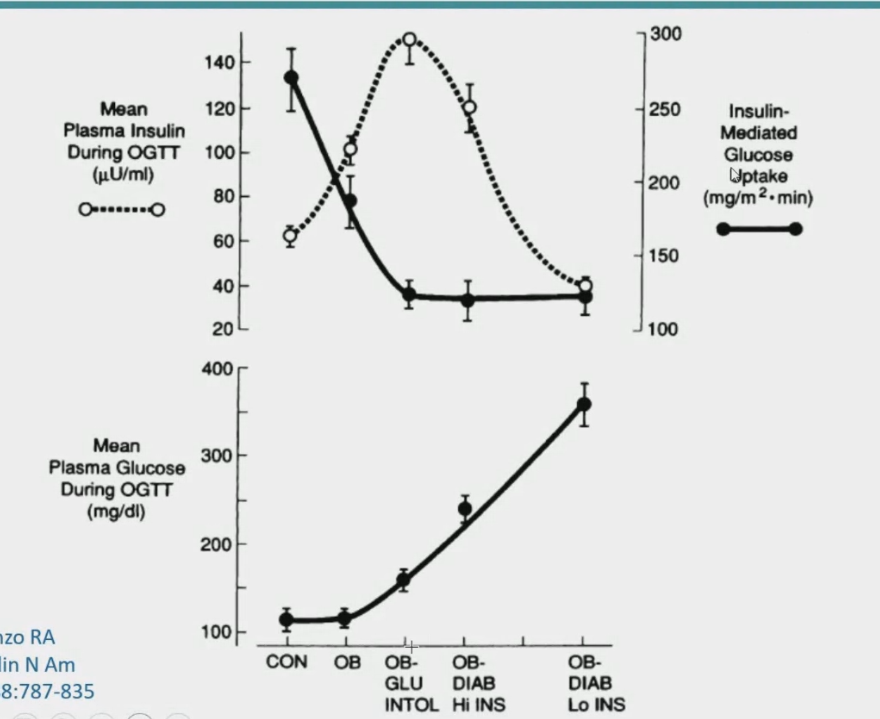
\includegraphics[width = 0.6 \textwidth]{Imagenes/InsulinaGlucosa.png}
    \caption{Relación de la glucosa e insulina por grado de enfermedad.}
    \label{fig:relGluIns}
\end{figure}

La Figura \ref{fig:relGluIns} fue tomada de una de las presentaciones de la Dra. Adriana Monroy. En ella se representan cinco grupos: el grupo control, personas con obesidad, personas con obesidad e intolerancia a la glucosa, personas con obesidad y diabetes con insulina alta, y personas con obesidad y diabetes con baja insulina. El objetivo es ilustrar cómo se comporta la interacción entre la glucosa e insulina dependiendo del estado de salud de los individuos.

En la gráfica de la parte inferior, se puede observar cómo, al empeorar la condición de salud, la media de los niveles de glucosa durante la prueba de tolerancia oral a la glucosa es más elevada. Este incremento en los niveles medios de glucosa refleja el deterioro progresivo en la regulación de la glucosa a medida que avanza la enfermedad.

Por otro lado, la gráfica de la parte superior muestra la captación de la glucosa medida por la insulina. En el grupo control, se observa que los niveles promedio de insulina en sangre son normales y la eficiencia de la insulina es buena. En el grupo de personas con obesidad, se puede ver cómo la producción de insulina es mayor, pero su eficiencia es menor, lo que indica posibles inicios de un trastorno metabólico.

A partir del grupo que presenta intolerancia a la glucosa, se puede observar cómo la eficiencia en la captación de glucosa llega a un límite. En las etapas siguientes, se evidencia el desgaste progresivo de las células beta del páncreas. En la última etapa, correspondiente a individuos con obesidad y diabetes con baja insulina, la producción de insulina es muy baja junto con su capacidad de absorción. Esto no solo refleja un deterioro avanzado en la regulación de la glucosa, sino también un agotamiento significativo de las células beta.

Estas observaciones subrayan la importancia de intervenir tempranamente en individuos con obesidad y aquellos que muestran signos de intolerancia a la glucosa. La progresión de la enfermedad desde la resistencia a la insulina hasta el agotamiento de las células beta resalta la necesidad de un monitoreo continuo y estrategias preventivas para evitar que la diabetes se vuelva irreversible.

%%%%%%%%%%%%%%%%%%%%%%%%%%%%%%%%%%%%%%%%%%%%%%%%%%
%%% A N A L I S I S  D E  R E S U L T A D O S %%%%
%%%%%%%%%%%%%%%%%%%%%%%%%%%%%%%%%%%%%%%%%%%%%%%%%%

\section{Interpretación de las Herramientas Visuales}

Dado el objetivo de crear un modelo simplificado, se va a construir un sistema que requiera un mínimo de variables, utilizando mediciones de fácil obtención. La variable de interés es $FBI/GC$, la cual se ha generado mediante el concepto de profundidad de banda con signo a partir de las curvas de glucosa e insulina, descrito en el Capítulo \ref{RegCuanDatosFun}. Las variables predictoras incluidas son los niveles de glucosa en ayunas y a los $120$ minutos durante la prueba de tolerancia a la glucosa oral, junto con el índice de masa corporal. Adicionalmente, se planea crear otro modelo al que se le añadirán mediciones de presión diastólica para explorar su efecto en la predicción de $FBI/GC$.

A continuación, se muestran las matrices de la $\sigma$ de Schweizer y Wolff, de hombres, mujeres y el total de la población, respectivamente. La correlación $\sigma$ de la variable respuesta el grupo de hombres es ligeramente mayor con todas las demás variables que en comparación con el caso de las mujeres.

\[
\sigma_{Muj} = \begin{blockarray}{cccccc}
FBI/GC      &      BMI      &    Glu.0      &  Glu.120      & PA.diast \\
\begin{block}{(ccccc)c}
1.000 & 0.311 & 0.542 &  0.733 & 0.181 & FBI/GC \\
0.311 & 1.000 & 0.304 &  0.308 & 0.261 & BMI \\
0.542 & 0.304 & 1.000 &  0.570 & 0.184 & Glu.0 \\
0.733 & 0.308 & 0.570 &  1.000 & 0.181 & Glu.120 \\
0.181 & 0.261 & 0.184 &  0.181 & 1.000 & PA.diast \\
\end{block}
\end{blockarray}
 \]

\[
\sigma_{Hom} = \begin{blockarray}{cccccc}
FBI/GC      &      BMI      &    Glu.0      &  Glu.120      & PA.diast \\
\begin{block}{(ccccc)c}
1.000 & 0.412 & 0.649 & 0.770 & 0.333 & FBI/GC \\
0.412 & 1.000 & 0.336 & 0.261 & 0.353 & BMI \\
0.649 & 0.336 & 1.000 & 0.591 & 0.312 & Glu.0 \\
0.770 & 0.261 & 0.591 & 1.000 & 0.282 & Glu.120\\
0.333 & 0.353 & 0.312 & 0.282 & 1.000 & PA.diast \\
\end{block}
\end{blockarray}
 \]


\[
\sigma_{Total} = \begin{blockarray}{cccccc}
FBI/GC      &      BMI      &    Glu.0      &  Glu.120      & PA.diast \\
\begin{block}{(ccccc)c}
1.000 & 0.361 & 0.567 & 0.747 & 0.244 & FBI/GC \\
0.361 & 1.000 & 0.324 & 0.320 & 0.317 & BMI \\
0.567 & 0.324 & 1.000 & 0.557 & 0.273 & Glu.0 \\
0.747 & 0.320 & 0.557 & 1.000 & 0.223 & Glu.120 \\
0.244 & 0.317 & 0.273 & 0.223 & 1.000 & PA.diast \\
\end{block}
\end{blockarray}
 \]

Todos los coeficientes resultantes de las matrices de correlación son lo suficientemente altos como para decir que hay algo que modelar con cópulas. De acuerdo con \cite{Erdely2022}, en este se enfatiza que si $\sigma_{C} = \rho_{C}$, entonces las variables aleatorias tienen una relación de dependencia de cuadrante positiva, y si $\sigma_{C} = -\rho_{C}$, entonces tienen una relación de dependencia de cuadrante negativa. Por otro lado, si $ |\rho_C| < \sigma_C$, significa que la dependencia es positiva en algunos cuadrantes y negativa en otros dentro del dominio de la cópula. Esto debido de a que $\rho_{C}$ es un valor promedio de dependencia del cuadrante, el cual podría ser cero.


La información anterior es beneficiosa durante el proceso de modelación, ya que una concordancia alta indica que el modelo paramétrico es capaz de capturar adecuadamente la estructura de dependencia entre las variables, mientras que una concordancia baja sugiere que el modelo podría no ser adecuado para describir la relación entre las variables. Además, es importante que el tipo de concordancia sea consistente en todo el dominio, ya que se requeriría de otras técnicas que pueden modelar este tipo de comportamiento, como el pegado de cópulas, entre otras.

A continuación, se muestran las matrices de diferencia:


\[
\sigma_{Muj} - \rho_{Muj} = \begin{blockarray}{cccccc}
FBI/GC      &      BMI      &    Glu.0      &  Glu.120      & PA.diast \\
\begin{block}{(ccccc)c}
  0.000 & 0.002 & -0.001 & -0.001  & -0.001 & FBI/GC \\
  0.002 & 0.000 &  0.002 &  0.004  & -0.001 & BMI \\
 -0.001 & 0.002 &  0.000 &  0.023  &  0.025 & Glu.0 \\
 -0.001 & 0.004 &  0.023 &  0.000  &  0.008 & Glu.120 \\
 -0.001 &-0.001 &  0.025 &  0.008  &  0.000 & PA.diast \\
\end{block}
\end{blockarray}
 \]

 \[
\sigma_{Hom} - \rho_{Hom} = \begin{blockarray}{cccccc}
FBI/GC      &      BMI      &    Glu.0      &  Glu.120      & PA.diast \\
\begin{block}{(ccccc)c}
0.000 & 0.004 & 0.002  & 0.000  & -0.003 & FBI/GC \\
0.004 & 0.000 & 0.007  & 0.013  &  0.002 & BMI \\
0.002 & 0.007 & 0.000  & 0.022  &  0.022 & Glu.0 \\
0.000 & 0.013 & 0.022  & 0.000  &  0.005 & Glu.120 \\
0.003 & 0.002 & 0.022  & 0.005  &  0.000 & PA.diast \\   
\end{block}
\end{blockarray}
 \]

 \[
\sigma_{Total} - \rho_{Total} = \begin{blockarray}{cccccc}
FBI/GC      &      BMI      &    Glu.0      &  Glu.120      & PA.diast \\
\begin{block}{(ccccc)c}
 0.000 & 0.002 & 0.002  & 0.000  &  0.008 & FBI/GC \\
 0.002 & 0.000 & 0.005  & 0.004  &  0.006 & BMI \\
 0.002 & 0.005 & 0.000  & 0.024  &  0.029 & Glu.0 \\
 0.000 & 0.004 & 0.024  & 0.000  &  0.016 & Glu.120 \\
 0.008 & 0.006 & 0.029  & 0.016  &  0.000 & PA,diast \\
\end{block}
\end{blockarray}
 \]

Las matrices de diferencias de los coeficientes $\rho$ de Spearman y $\sigma$ de Schweizer y Wolff presentadas anteriormente muestran valores muy bajos, lo cual indica que las dependencias entre las variables tienen un tipo de monotonía a lo largo de todo su dominio, es decir, son únicamente crecientes o decrecientes. Esta característica es beneficiosa al momento de ajustar cópulas, ya que sugiere que las cópulas paramétricas son una opción adecuada para modelar estas dependencias. Por esta razón, el modelo D-vine que se va a construir estará ajustado exclusivamente con cópulas paramétricas. Este enfoque permite capturar de manera efectiva las relaciones monotónicas entre las variables, mejorando la precisión y la interpretabilidad del modelo.



%%%%%%%%%%%%%%%%%%%%%%%%%%%%%%%%%%%%%%%%%%%%%%%%%%
%%%%%%%%%%%%%%%%%%%%%%%%%%%%%%%%%%%%%%%%%%%%%%%%%%

\subsection{Gráficos de dispersión y Heatmaps}

Para obtener una comprensión más profunda de cómo se ajusta cada cópula, se emplearon visualizaciones propuestas por Arturo Erdely y Manuel Rubio-Sanchez en \cite{Erdely2022}. Estas visualizaciones ofrecen una nueva perspectiva al representar la clásica gráfica de puntos de una manera innovadora, y al resaltar las diferencias entre la cópula empírica y la cópula independiente. Estas herramientas visuales ayudan a identificar patrones y estructuras de dependencia en los datos, lo que facilita la evaluación del ajuste de las cópulas y el análisis de la relación entre las variables. 

Recordando que las medidas $\rho_C$ y $\sigma_C$ se obtienen de medir la distancia entre la cópula empírica y la independiente, se proponen los heatmaps $\mathscr{H}_\rho$ y $\mathscr{H}_\sigma$ definidos en las ecuaciones \eqref{Hrho} y \eqref{Hsigma}, respectivamente, que visualizar esta distancia en distintos puntos del dominio de la cópula. Adicionalmente se propone el heatmap $\mathscr{H}$ definido en \eqref{H}, el cual muestra la distancia entre la cópula empírica y la independiente, con respecto a la cercanía con los limites de Frechet -Hoeffding:

\begin{equation}\label{Hrho}
    \mathscr{H}_\rho=\left\{12\left[C_n\left(\frac{i}{n}, \frac{j}{n}\right)-\frac{i j}{n^2}\right]: i, j \in\{1, \ldots, n-1\}\right\},
\end{equation}

\begin{equation}\label{Hsigma}
    \mathscr{H}_\sigma = \left\{12\left|C_n\left( \frac{i}{n}, \frac{j}{n}\right)-\frac{i j}{n^2}\right|: i, j \in\{1, \ldots, n-1\}\right\},
\end{equation}


\begin{equation}\label{D}
    D_n\left(\frac{i}{n}, \frac{j}{n}\right)=\left\{\begin{array}{cc}
\frac{C_n\left(\frac{i}{n}, \frac{j}{n}\right)-\Pi\left(\frac{i}{n}, \frac{j}{n}\right)}{M\left(\frac{i}{n}, \frac{j}{n}\right)-\Pi\left(\frac{i}{n}, \frac{j}{n}\right)} & \text { if } C_n\left(\frac{i}{n}, \frac{j}{n}\right) \geq \Pi\left(\frac{i}{n}, \frac{j}{n}\right), \\
-\frac{\Pi\left(\frac{i}{n}, \frac{j}{n}\right)-C_n\left(\frac{i}{n}, \frac{j}{n}\right)}{\Pi\left(\frac{i}{n}, \frac{j}{n}\right)-W\left(\frac{i}{n}, \frac{j}{n}\right)} & \text { if } C\left(\frac{i}{n}, \frac{j}{n}\right)<\Pi\left(\frac{i}{n}, \frac{j}{n}\right),
\end{array}\right. \quad \text{ para } i,j \in  \left\{ 1, \dots, n-1 \right\} 
\end{equation}

\begin{equation}\label{H}
    \mathscr{H} =\left\{ D_n\left( \frac{i}{n}, \frac{j}{n}\right) : i, j \in\{1, \ldots, n-1\}\right\}.
\end{equation}


Para iniciar con una visualización clásica, en la Figura \ref{fig:diagE} se muestran los gráficos de dispersión de las covariables dos a dos de los datos proveninetes de mujeres en escala $u$. En la diagonal superior se presentan las dispersión de las variables, mientras que en la diagonal inferior se muestran las diagonales de diferentes cópulas. La curva roja representa la diagonal de la cópula $W$, que corresponde a la cota inferior; en azul, se encuentra la diagonal de la cópula independiente; en verde la diagonal de la curva superior $M$, la cota superior; y por último, en negro se grafica la diagonal de la función empírica. Esta visualización ayuda a comprender las relaciones de concordancia presentes en cada variable, lo que facilita la elección de una estrategia adecuada al modelar con cópulas.

\begin{figure}[H]
    \centering
    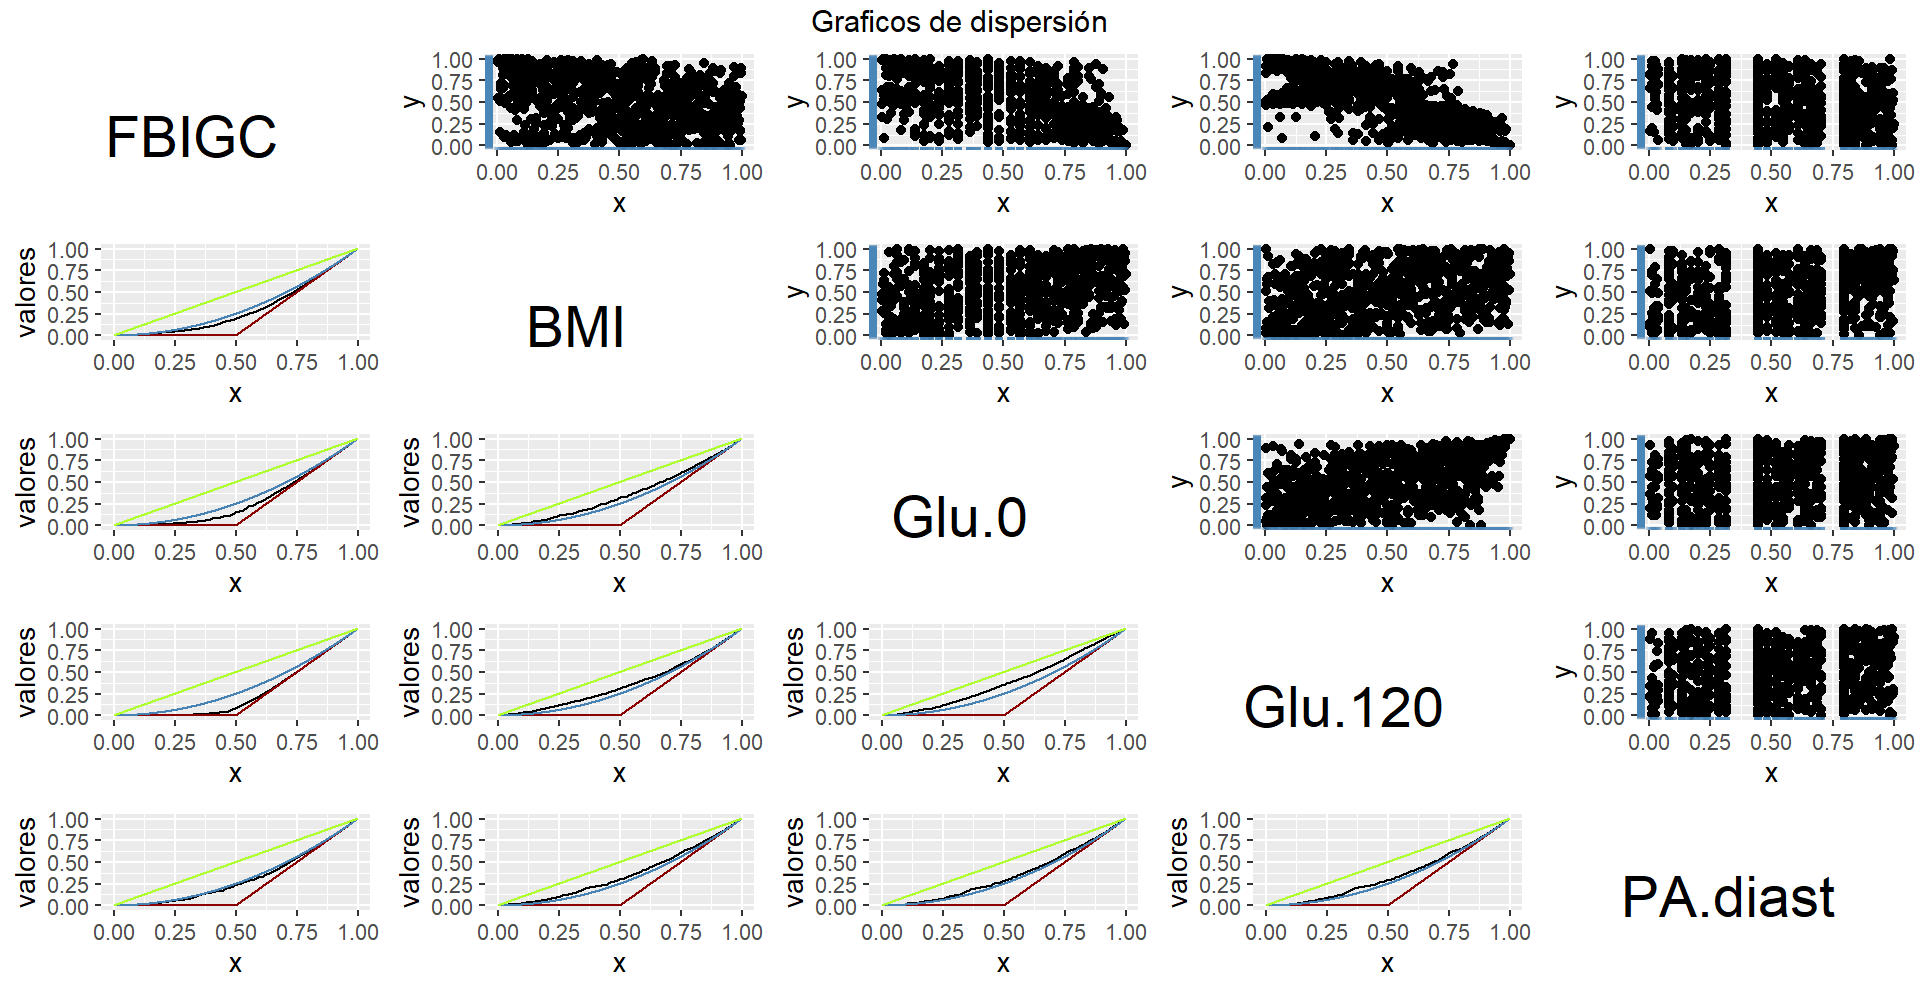
\includegraphics[width = 0.97 \textwidth]{4img/UdiagM.png}
    \caption{Diagonales y gráficos de dispersión en escala $u$.}
    \label{fig:diagE}
\end{figure}

Es importante tener en cuenta que aún falta explorar las dependencias entre las variables condicionales. Aunque los gráficos de dispersión proporcionan una visión general, también revelan ciertas franjas en los datos, lo cual puede indicar limitaciones potenciales del modelo (ver la diagonal superior de la Figura \ref{fig:diagE}). Esto se debe a que la mayoría de las cópulas paramétricas asumen datos continuos, y la presencia de franjas en los datos podría afectar la capacidad del modelo para capturar la verdadera estructura de dependencia entre las variables. Por lo tanto, es necesario realizar un análisis más detallado para comprender completamente la naturaleza de las dependencias y evaluar la idoneidad del modelo propuesto.

Ahora se aplicará los heatmaps anteriores a cópulas D-Vine. Para simplificar la notación del modelo D-vine, en lugar de escribir todos los árboles, solo se utilizará el árbol del primer nivel ya que este determina todas las estructuras subsecuentes, representándolo como un modelo aditivo. Esto se debe a su facilidad de comprensión y a la capacidad de trabajar con él en el entorno de fórmulas de \texttt{R}. Sin embargo, es importante tener en cuenta que esto no significa que en el modelado se asuma que las relaciones son aditivas. En realidad, se modelan las relaciones a pares de cópulas, lo que permite capturar una gama más amplia de estructuras de dependencia entre las variables.

En general, se asignará a cada variable que se modela un número, correspondiente al orden en el que el modelo D-vine las ajusta. Por ejemplo, en el modelo $FBI/GC \sim GLU.120 + GLU.0 + IBM + PA.diast$, la variable $1$ corresponderá a la variable respuesta $FBI/GC$, la variable $2$ a $Glu.120$, y así sucesivamente. Cuando se modele la dependencia entre dos variables utilizando cópulas, se utilizará el número de variable como subíndice. Por ejemplo, $C_{12}$ representaría la cópula entre $FBI/GC$ y $Glu.120$.


\begin{figure}[H]
 \centering
  \subfloat[$\mathscr{H}\rho$]{
   \label{rhoT}
    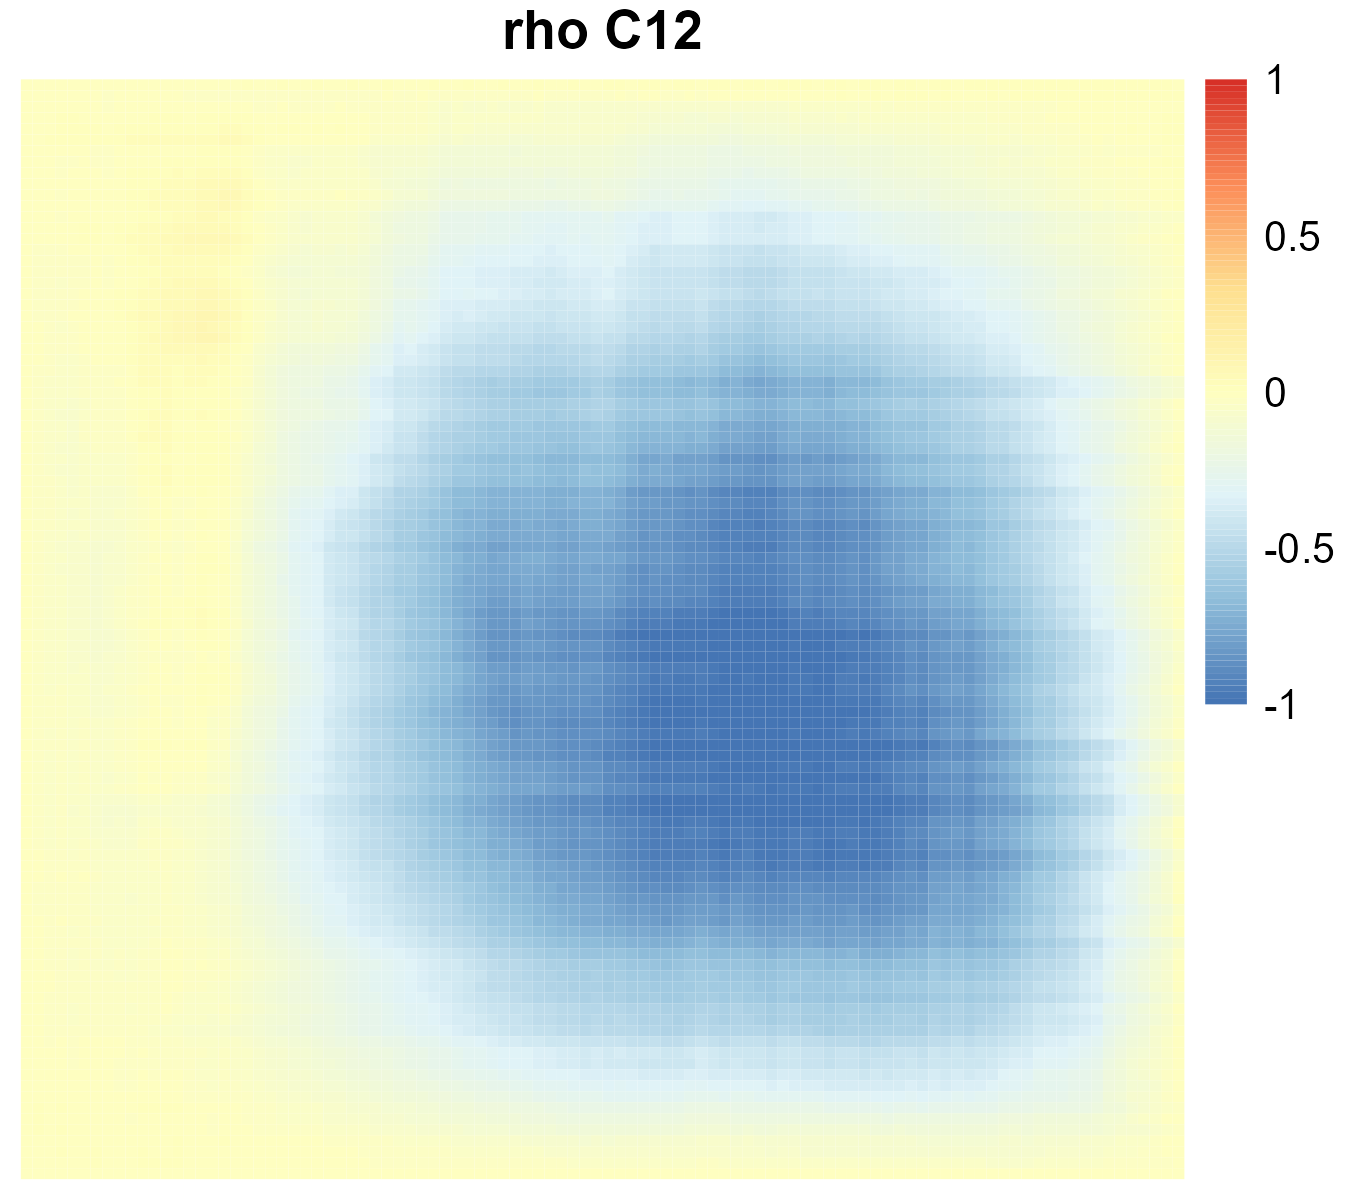
\includegraphics[width=0.32\textwidth]{4img/TotalrhoC12.png}}
  \subfloat[$\mathscr{H}\sigma$]{
   \label{sigmaT}
    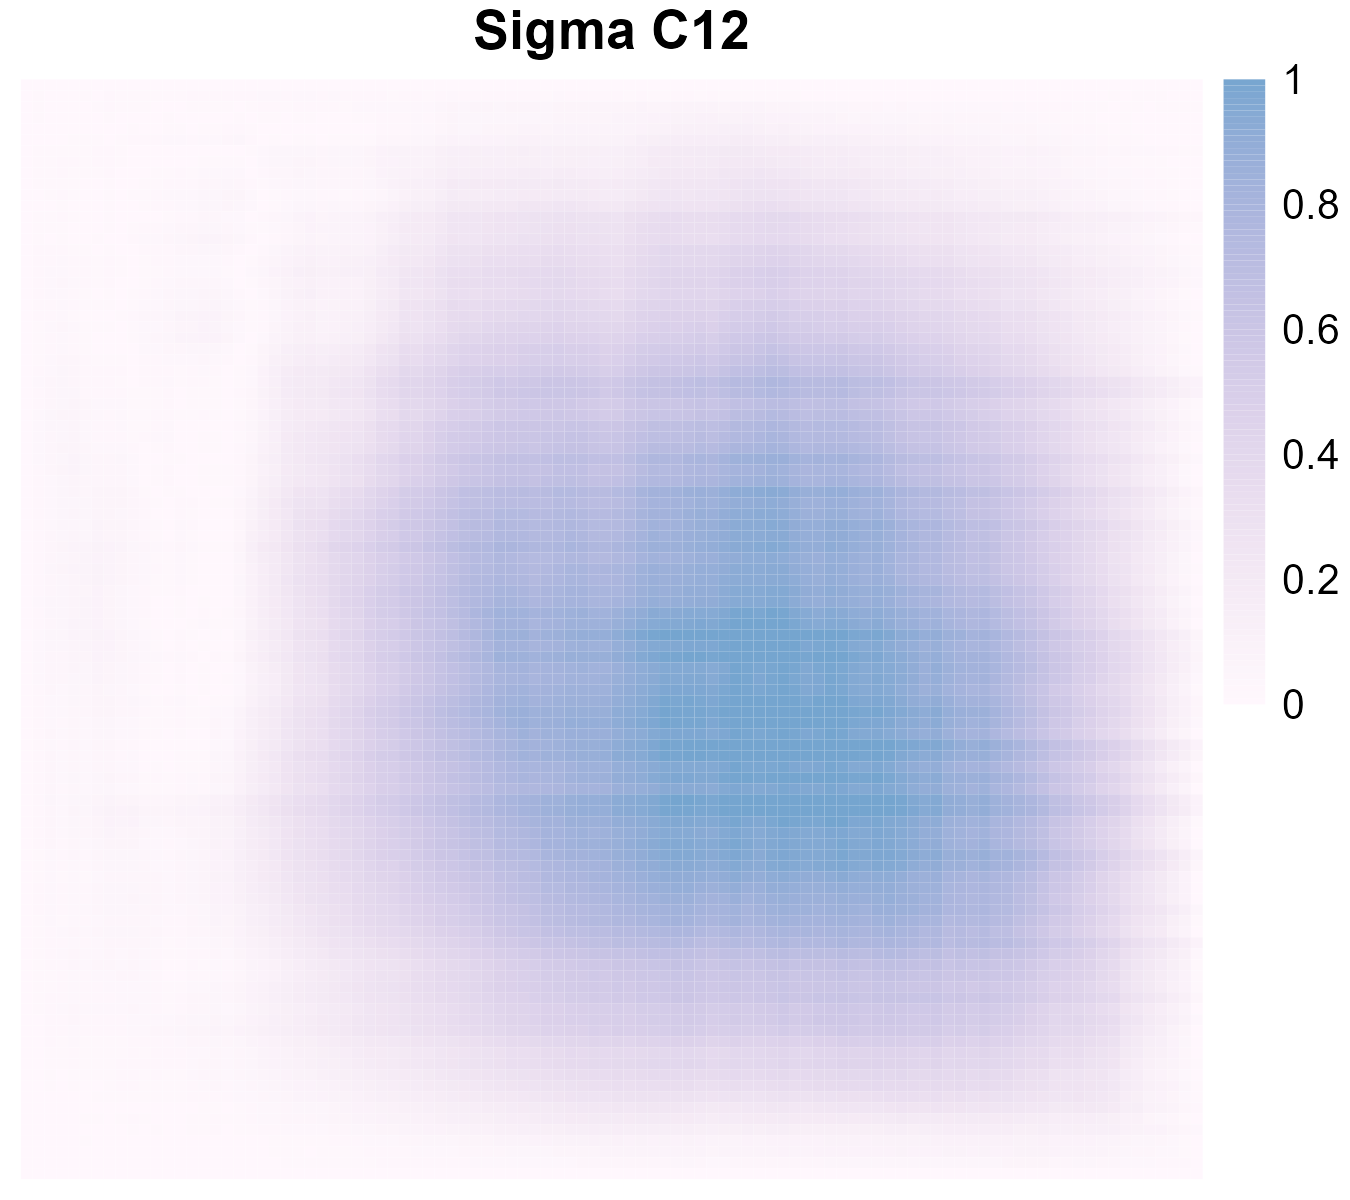
\includegraphics[width=0.32\textwidth]{4img/TotalsigmaC12.png}}
  \subfloat[$\mathscr{H}$]{
   \label{HT}
    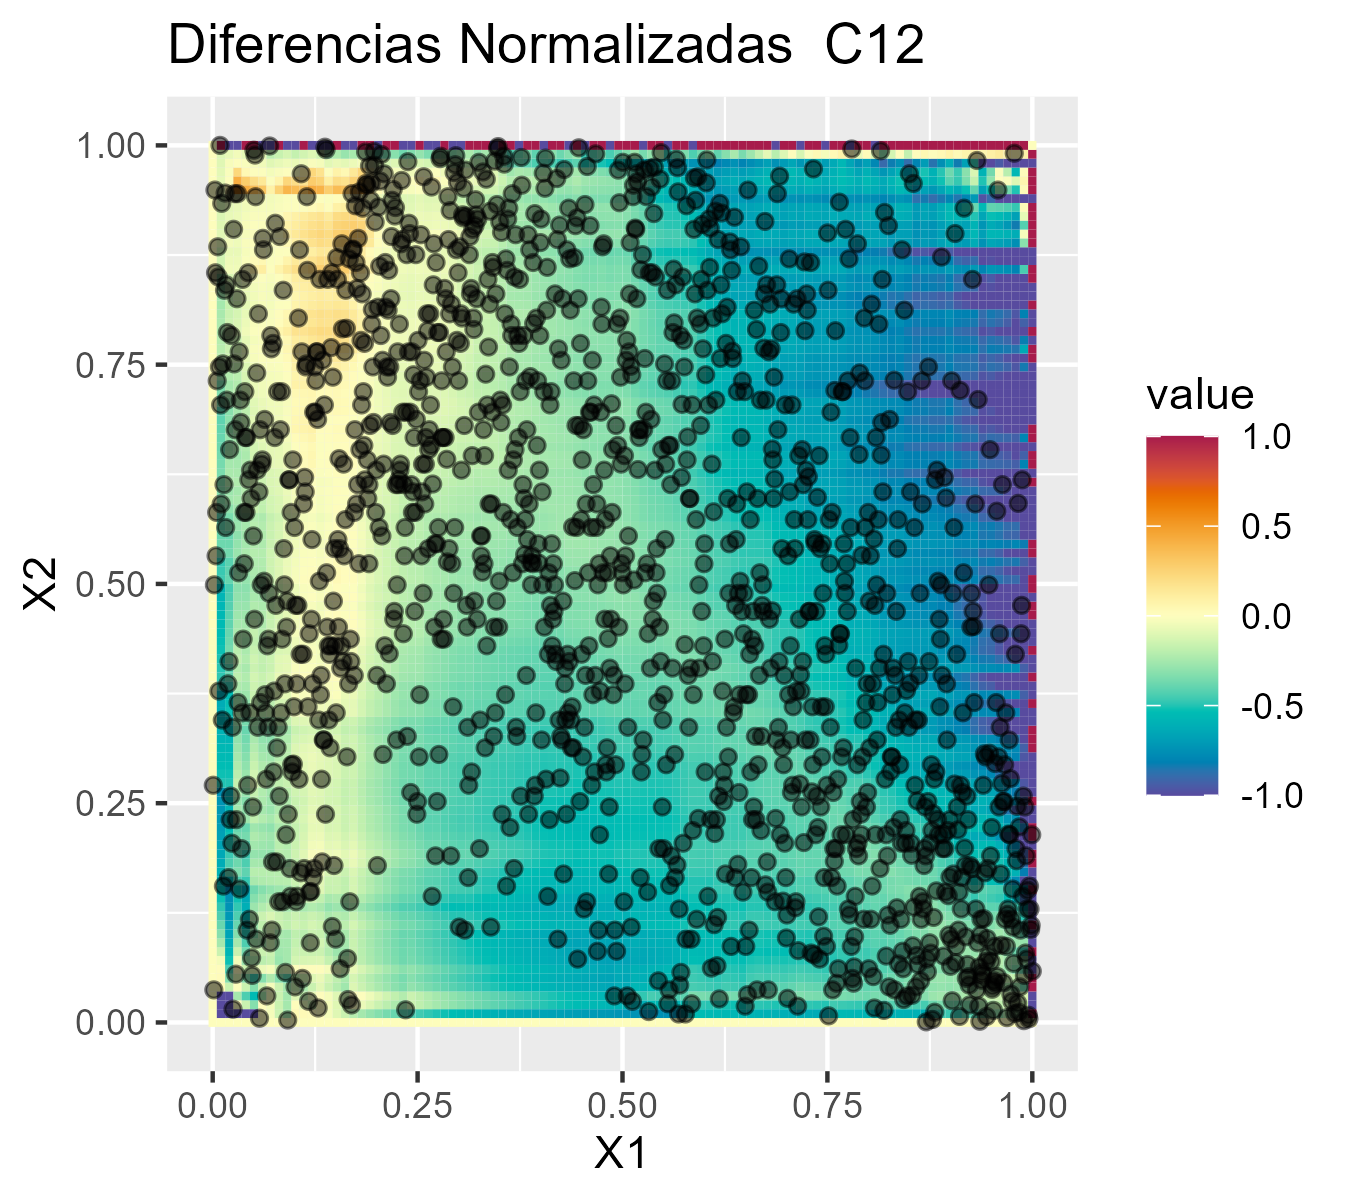
\includegraphics[width=0.32\textwidth]{4img/TotalHC12.png}}
    \caption{Ejemplo de Heatmaps}
    \label{heatEj}
\end{figure}

La Figura \ref{heatEj} presenta los heatmaps \eqref{Hrho}, \eqref{Hsigma} y \eqref{H} aplicados a la cópula entre $FBI/GC$ y $Glu.120$ para la cópula D-vine discutida arriba; más detalles sobre el ajuste de este modelo se presentan abajo. Como guía para interpretar los heatmaps, en la primera columna de la Figura \ref{heatEj}, se muestra la medida $\rho_C$ de Spearman en una cuadrícula de $100$ por $100$ en el intervalo $[0, 1]^2$. Las áreas azules indican que la distancia entre la cópula empírica evaluada en el punto $(u, v)$ está por debajo de la cópula independiente. Por otro lado, si los valores son positivos, esto indicará que la cópula empírica está por encima de la cópula independiente y su color será rojo. Este gráfico ayuda a visualizar el comportamiento de la cópula en todo el dominio, proporcionando información sobre la dirección y la magnitud de las diferencias entre la cópula empírica y la independiente.

En la segunda columna de la Figura \ref{heatEj}, se encuentra el heatmap con la medida $\sigma_C$. Esta medida solo evalúa la distancia entre la cópula empírica y la independiente sin considerar su signo. Esto nos ayuda a visualizar la magnitud de la dependencia en todo el dominio de la cópula, proporcionando una representación clara de la fuerza de la relación entre las variables.

Finalmente, el heatmap de la tercera columna de la Figura \ref{heatEj}, muestra las diferencias con normalización. Esto permite observar la presencia de tendencias crecientes y decrecientes en la relación entre las variables. Además, se sobreponen los datos con los que se estimó la cópula para ofrecer mayor claridad en la interpretación de los datos, lo que facilita la identificación de patrones y estructuras de dependencia en el conjunto de datos analizado.

%%%%%%%%%%%%%%%%%%%%%%%%%%%%%%%%%%%%%%%%%%%%%%%%%%%%%%%%%%%%%
%%%%%%%%%%%%%%%%%%%%%%%%%%%%%%%%%%%%%%%%%%%%%%%%%%%%%%%%%%%%%

\subsection{Tabla Resumen de Pertenencia a cada Clase}\label{subTabla}

Para generalizar el modelo, se separan a los individuos según su prediagnóstico, que proviene de la información de glucosa en los tiempos $0$ y $120$, así como su clasificación de nivel de obesidad según el Índice de Masa Corporal. A continuación se mencionan estas categorías propuesta por el Dr. Arnulfo González Cantú:

\begin{multicols}{2}
    \begin{itemize}
        \item Normal-Peso Normal
        \item Normal-Sobrepeso
        \item Normal-Obesidad	
        \item Prediabetes-Peso Normal
        \item Prediabetes-Sobrepeso
        \item Prediabetes-Obesidad	
        \item Diabetes-Peso Normal	
        \item Diabetes-Sobrepeso
        \item Diabetes-Obesidad
    \end{itemize}
\end{multicols}

Al categorizar a los individuos de esta manera, se puede analizar la relación entre las variables en diferentes subgrupos, lo que puede ayudar a identificar patrones específicos y a adaptar el modelo a las necesidades particulares de cada grupo.

Dividiendo a los individuos en las clasificaciones mencionadas anteriormente, se puede obtener la mediana de cada covariable para cada grupo y luego ingresar estas medianas al modelo para calcular la probabilidad de pertenecer a cada clase del $FBI/GC$, que incluyen las siguientes categorías: completamente sanos, resistencia a la insulina con predisfunción de célula beta, resistencia a la insulina con estrés de célula beta y resistencia a la insulina con disfunción obvia de célula beta. Este enfoque nos permite evaluar cómo varían las probabilidades de pertenecer a cada clase según las características de los individuos, lo que puede proporcionar información valiosa para la detección temprana y la intervención en diferentes estados de salud relacionados con la glucosa y la obesidad.

La tabla resultante del trabajo descrito anteriormente es fácilmente manejable y se puede utilizar de la siguiente manera:

\begin{enumerate}
    \item Ubicar la fila que corresponde a cada individuo colocando las medidas de glucosa en el tiempo $0$ ($Glu.0$), en el tiempo $120$ ($Glu.120$) y el Índice de Masa Corporal ($BMI$), de acuerdo a las clasificaciones descritas \ref{ClasificaVar}.

    \item En las columnas $C_1$, $C_2$, $C_3$, $C_4$, se muestran las probabilidades correspondientes a cada clase del $FBI/GC$ (completamente sanos, resistencia a la insulina con predisfunción de célula beta, resistencia a la insulina con estrés de célula beta y resistencia a la insulina con completa disfunción de célula beta, respectivamente).
\end{enumerate}

En la Figura \ref{fig:ejemploTabla}, se muestra un ejemplo. Esta tabla facilita la evaluación de las probabilidades de pertenecer a cada clase del $FBI/GC$ para diferentes combinaciones de glucosa y $BMI$, lo que permite una rápida identificación de los grupos de riesgo y la toma de decisiones informadas sobre la salud y el tratamiento. Estas predicciones de cada grupo de pacientes se obtuvieron tomando la mediana de cada covariable por cada grupo.

\begin{figure}[H]
    \centering
    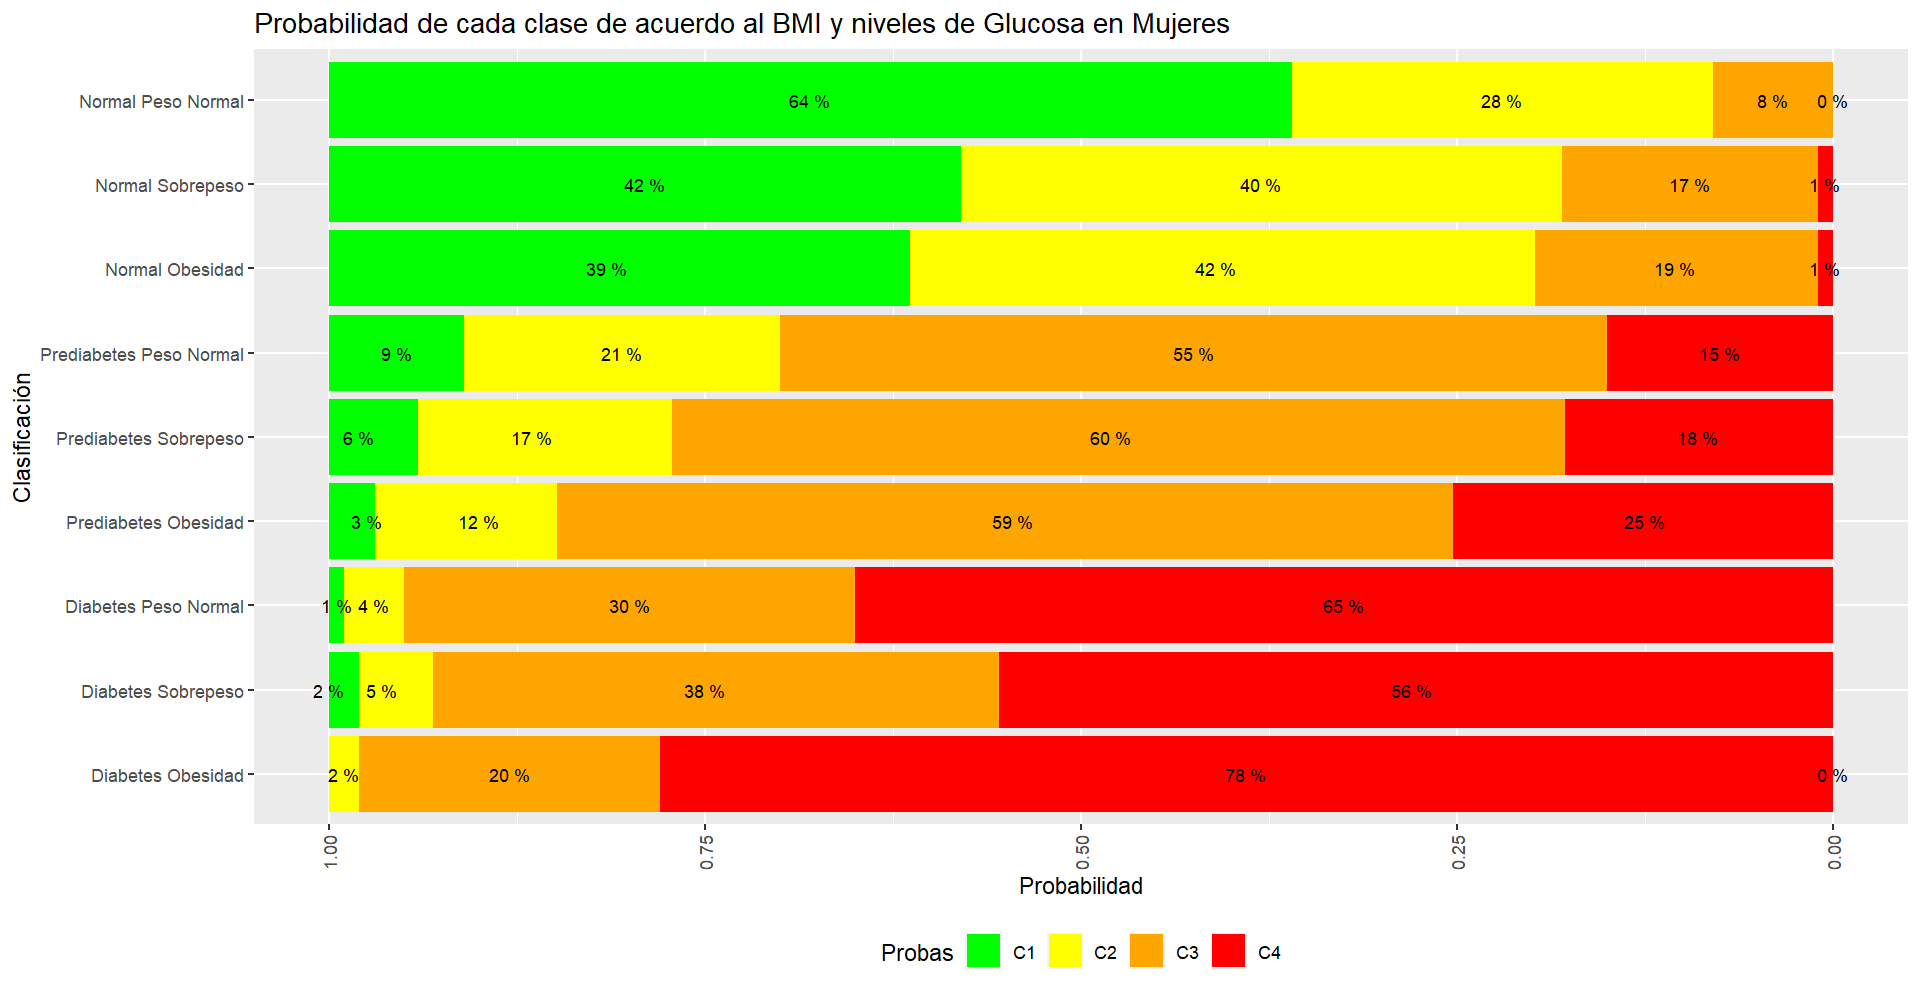
\includegraphics[height = 12 cm, width = 0.98 \textwidth]{4img/tablaM.png}
    \caption{Tabla de probabilidades de cada clase.}
    \label{fig:ejemploTabla}
\end{figure}

Para el cálculo de las probabilidades en esta tabla, solo se calcularon las siguientes probabilidades:

\begin{equation}
     \begin{matrix}
\mathbb{P}[0 \leq Y \leq 1] = C_1 \\
\mathbb{P}[-1 \leq Y \leq 0] = C_2  \\
\mathbb{P}[-2 \leq Y \leq -1] = C_3 \\
\mathbb{P}[-3 \leq Y \leq -2] = C_4 \\
\end{matrix}
\end{equation}
%%%%%%%%%%%%%%%%%%%%%%%%%%%%%%%%%%%%%%%%%%%%%%%%%%%%%%
%%%%%%%%  g r a f i c a   d e  e f e c t o s %%%%%%%%%
%%%%%%%%%%%%%%%%%%%%%%%%%%%%%%%%%%%%%%%%%%%%%%%%%%%%%%

\subsection{Gráfica de Efectos}

Las gráficas de efectos ofrecen una herramienta valiosa para visualizar el impacto marginal de un predictor en el estimador cuantil. Estas representaciones permiten observar cómo varía el estimador cuantil en respuesta a cambios en un predictor específico, mientras se mantienen los demás predictores constantes a su valor promedio \cite{Tepegjozova2022}.

Para generar estas gráficas, se selecciona la variable $x_i$ de interés cuyo efecto se desea visualizar en la regresión. Luego, se calcula el promedio muestral de todas las otras variables como una estimación de la esperanza de cada una. De esta manera, solo es de interés el comportamiento de la variable respuesta $y$ cuando la variable $x_i$ varia, mientras que todas las demás variables se mantienen constantes en su valor promedio. Posteriormente, se realiza la regresión cuantil utilizando estos valores fijos para las variables control.

A continuación, se presenta un ejemplo del rendimiento de la gráfica de efectos. Se llevó a cabo la regresión cuantil para tres cuantiles diferentes: $\alpha = 0.1$, $0.5$ y $0.9$. Luego, se utilizó la función $geom\_smooth()$ para trazar una curva suave utilizando B-splines con 5 puntos internos. 

\begin{figure}[H]
 \centering
  \subfloat[Mujeres]{
   \label{ejEfec1}
    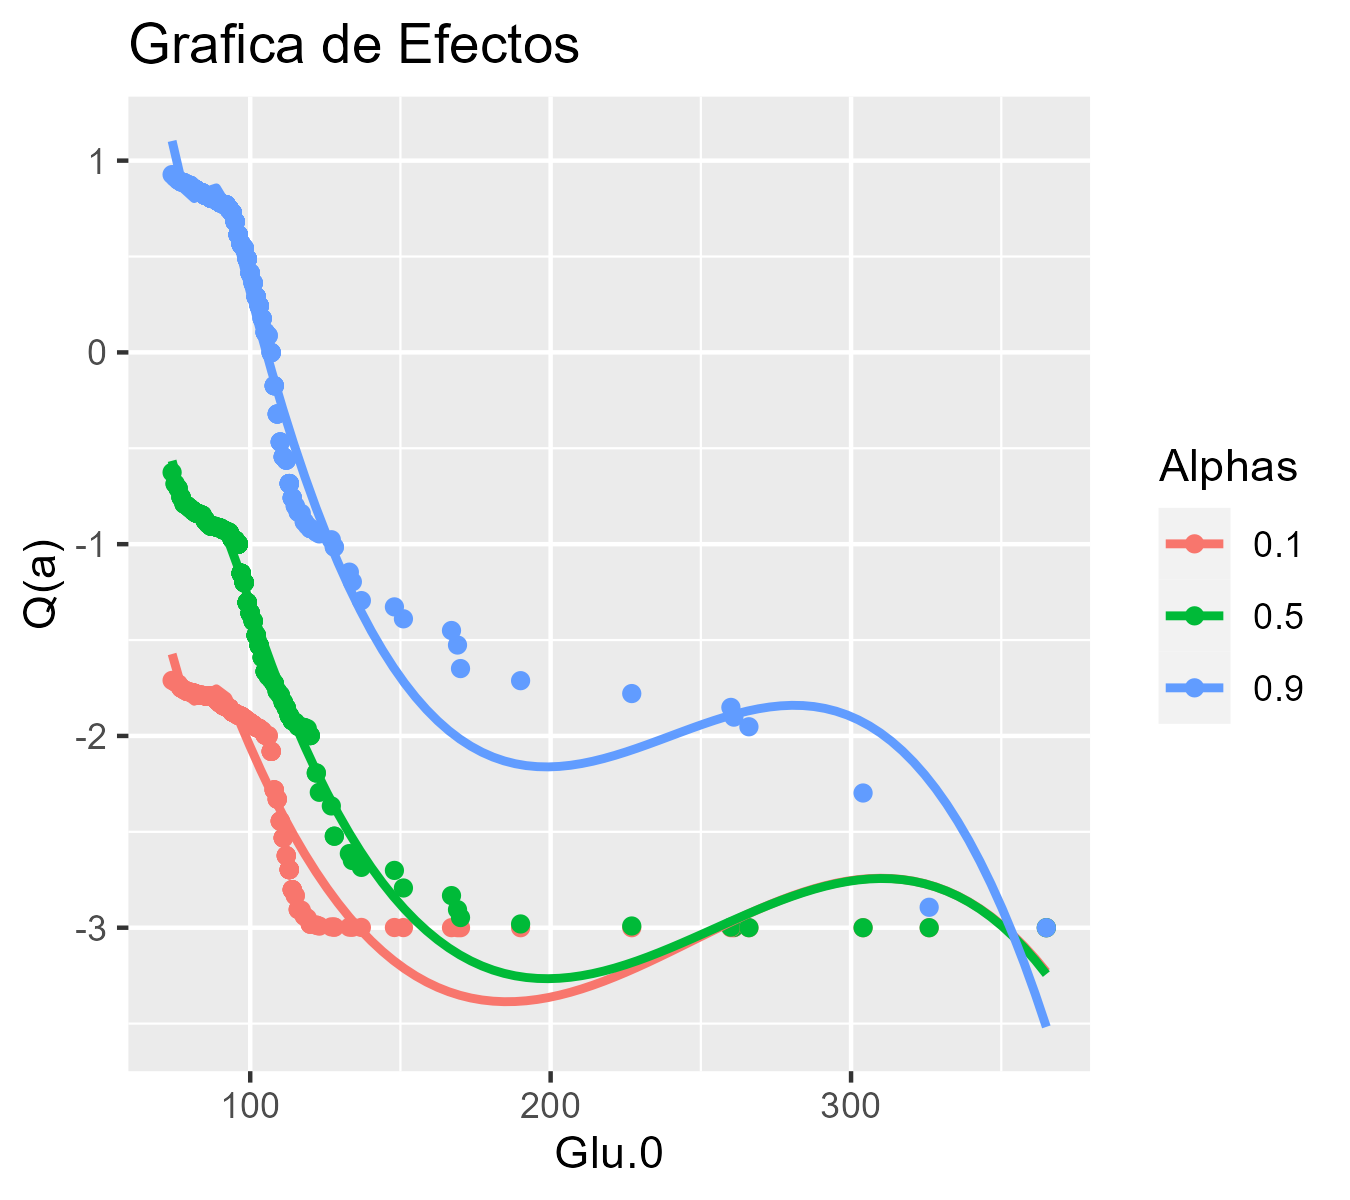
\includegraphics[width=0.45\textwidth]{4img/HomGlu.0Efec.png}}
  \subfloat[Hombres]{
   \label{ejEfect2}
    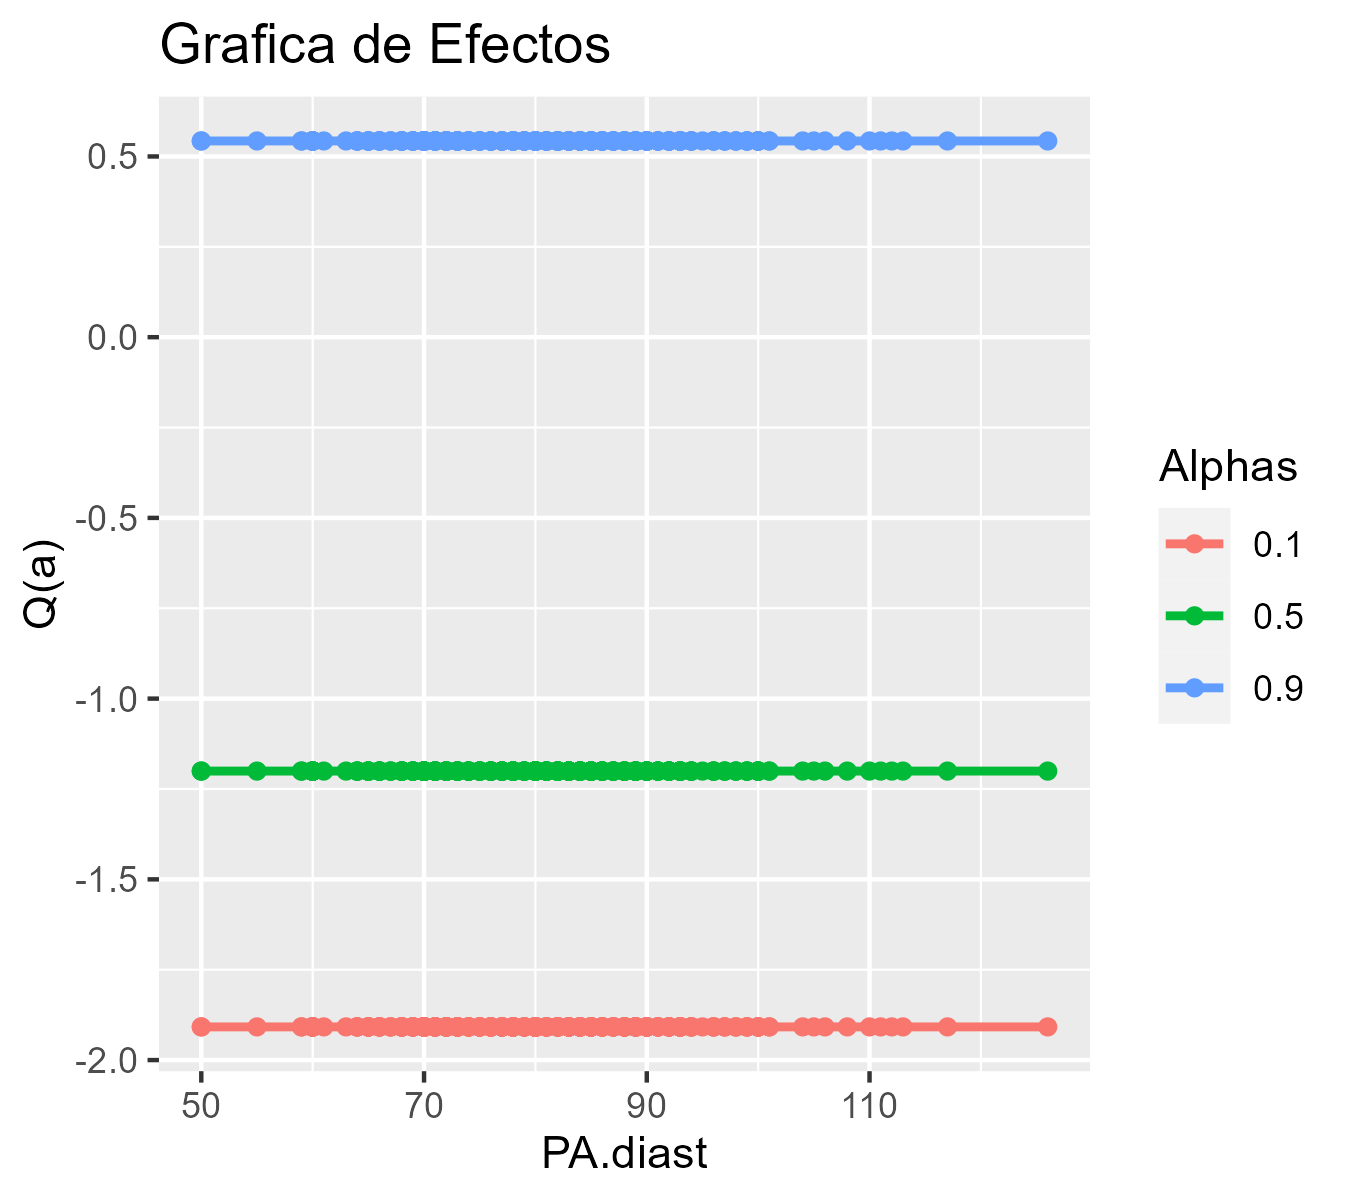
\includegraphics[width=0.45\textwidth]{4img/HomPA.diastEfec.png}}
    \caption{Ejemplos de las gráficas de efectos.}
    \label{fig:Efectos}
\end{figure}

En la Figura \ref{ejEfec1}, se ilustra cómo cambia la variable respuesta en función de los distintos valores de la variable $Glu.0$. Esto se puede entender como un boxplot continuo y puede ayudar a visualizar cómo varía la respuesta entre diferentes configuraciones del sistema. Al observar los boxplots, se puede identificar rápidamente qué configuraciones resultan en respuestas más consistentes (menor variabilidad) y cuáles tienen tiempos de respuesta más rápidos (mediana más baja). Por ejemplo, al final de esta gráfica, los datos también representan casos atípicos para la covariable que se está variando. Sin embargo, la respuesta deja de variar en estos casos debido a la menor cantidad de datos y la condición médica específica. Esta disminución en la variabilidad puede indicar que, en estas condiciones extremas, la respuesta se vuelve más uniforme, posiblemente debido a limitaciones fisiológicas.


Por otro lado, en la Figura \ref{ejEfect2}, se muestra el efecto de una variable que no aporta información al modelo. A medida que la covariable $PA.diast$ varía, no se refleja ningún cambio en la predicción; esto permanece constante. Esto indica que  $pA.diast$ no aporta información significativa a la regresión. La ausencia de variación en la respuesta sugiere que esta covariable no está relacionada con la variable de interés y, por lo tanto, no contribuye a mejorar el modelo predictivo. Identificar tales variables es crucial para simplificar el modelo y mejorar su interpretabilidad y eficiencia.


Este gráfico es herramienta fundamental en el análisis de resultados debido a su capacidad para visualizar de manera efectiva la variabilidad y la relación entre una covariable y la variable respuesta. En particular, permiten identificar patrones claros en los datos, como la consistencia en la respuesta frente a diferentes condiciones de una covariable o la falta de efecto de ciertas variables sobre la predicción. Esta capacidad de identificación es crucial para la selección de variables relevantes en los modelos predictivos y para mejorar la interpretación y la precisión de los resultados obtenidos. 

%%%%%%%%%%%%%%%%%%%%%%%%%%%%%%%%%%%%%%%%%%%%%%%%%%%%%%%%%%%%%%%%
%%%%%%%%%%%%%%%%%%%%%%%%%%%%%%%%%%%%%%%%%%%%%%%%%%%%%%%%%%%%%%%%

\vspace{-0.2cm}
\section{Librería deerVineReg}

\vspace{-0.3cm}
Todas las herramientas gráficas descritas anteriormente para evaluar y visualizar el desempeño del modelo ajustado fueron implementadas en el paquetería \textbf{deerVineReg}, la cuál se puede encontrar y descargar en github \url{https://github.com/BesitosDeBaba/deerVineReg}, uno de los principales objetivos de esta tesis. Existen otros paquetes, como \textbf{vineReg}, cuya utilidad se centra más en visualizar las dependencias dentro de un conjunto de variables, similar a la función de la PCA. Sin embargo, este proyecto se enfocó en desarrollar una paquetería orientada a un modelo predictivo de Machine Learning, con el objetivo de expandir el uso de modelos basados en cópulas.

El paquete \textbf{deerVineReg} no solo facilita la creación de modelos predictivos robustos utilizando cópulas, sino que también incluye herramientas avanzadas de visualización para interpretar los resultados y evaluar el desempeño del modelo. Esto permite a los usuarios no solo construir modelos precisos, sino también comprender mejor las relaciones subyacentes entre las variables y su impacto en la predicción. \textbf{deerVineReg} representa un avance significativo en el uso de cópulas para la predicción, ofreciendo una alternativa poderosa y accesible para la comunidad científica y médica.

%%%%%%%%%%%%%%%%%%%%%%%%%%%%%%%%%%%%%%%%%%%%%%%%%%%%%%%%%%%%%
%%%%%%%%%%%%%%%%%%%%%%%%%%%%%%%%%%%%%%%%%%%%%%%%%%%%%%%%%%%%%
\section{Modelos de 4 variables}

El orden de los tres modelos modelos construidos para el diagnóstico de la resistencia a la insulina en mujeres, hombres y para ambos sexos es

\vspace{-0.5cm}
\begin{equation}\label{ordenVar4}
     FBI/GC \sim Glu.120 + Glu.0 + BMI + PA.diast.
\end{equation}

Las cópulas ajustadas para los datos de mujeres se ilustran en la Figura \ref{fig:copulasTestMu}, mientras que las correspondientes a hombres se muestran en la Figura \ref{fig:copulasTestHo}.


Para ajustar las cópulas a pares de todos los niveles, se utilizó la función \textit{BiCopSelect} de la librería \textbf{VineCopula}. En las Figuras  \ref{fig:copulasTestMu}, \ref{fig:copulasTestHo} y \ref{fig:copulasTestTotal}, se muestran los nombres y parámetros, junto con el test de independencia ($H_0 =$ no hay depedencia) de las cópulas ajustadas dentro del modelo D-vine de mujeres, hombres y ambos sexos, respectivamente. Estos resultados permiten evaluar la idoneidad de las cópulas seleccionadas para modelar las relaciones entre las variables y determinar si existe alguna dependencia significativa entre ellas en cada grupo de datos, en caso de no haber desecharla. 

Para los tests de independencia se tomará un nivel de significancia de $\alpha = 0.05$. Esto significa que cualquier $p-valor$ que sea menor o igual a $0.05$ indicará que se rechaza la hipótesis nula de independencia entre las variables, lo que sugiere que hay una dependencia significativa entre ellas.

\begin{figure}[H]
 \centering
  \subfloat[Parte 1]{
   \label{ajusteMu1}
    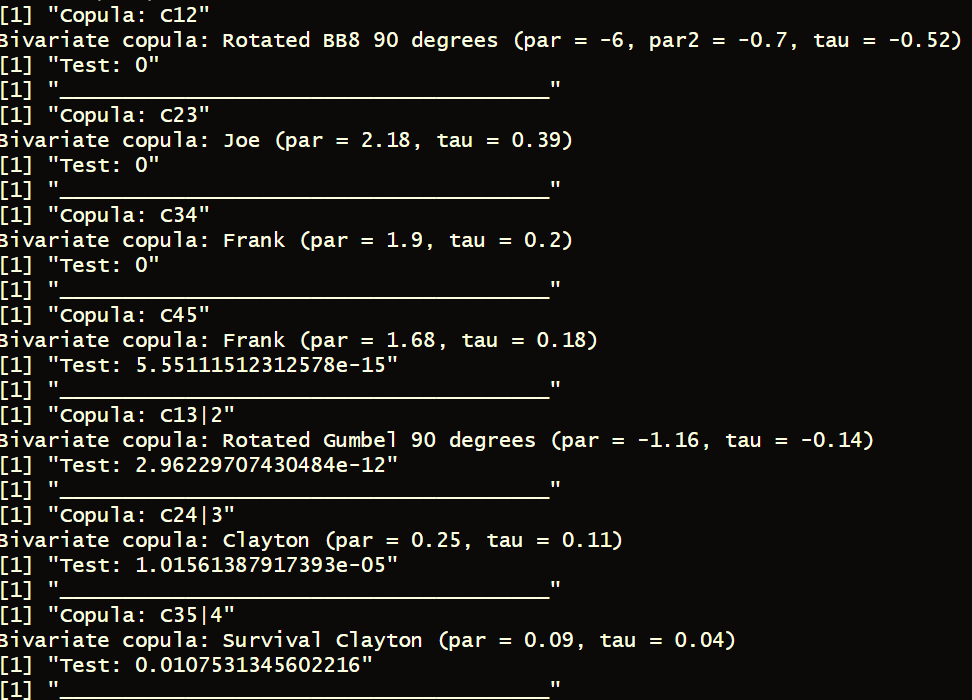
\includegraphics[width=0.46\textwidth]{4img/testM1.png}}
  \subfloat[Parte 2]{
   \label{ajusteMu2}
    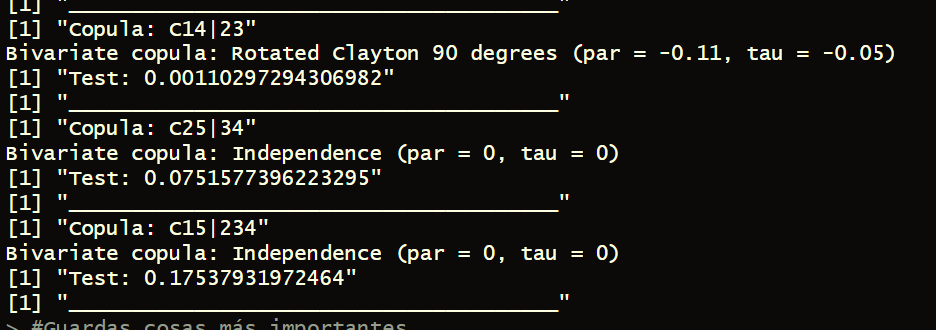
\includegraphics[width=0.46\textwidth]{4img/testM2.png}}
    \caption{Cópulas ajustadas la base de mujeres.}
    \label{fig:copulasTestMu}
\end{figure}
\vspace{-0.3cm}

Los tests de independencia de las cópulas ajustadas a los datos de mujeres que se muestran en la Figura \ref{fig:copulasTestMu}. Se puede observar en los niveles más bajos, como $C_{25|34}$ y $C_{15|234}$, muestran valores altos. Esto sugiere que podría ser beneficioso reducir una variable en estos niveles para mejorar la capacidad del modelo para capturar las relaciones entre las covariables. Los $p-valores$ relativamente altos para el test de independencia indican que las variables incluidas en estos pares de cópulas podrían no estar contribuyendo significativamente a la relación modelada. Por lo tanto, considerar la eliminación de una variable en estos niveles podría simplificar el modelo sin perder información importante sobre la dependencia entre las variables.

\begin{figure}[H]
 \centering
  \subfloat[Parte 1]{
   \label{ajusteHo1}
    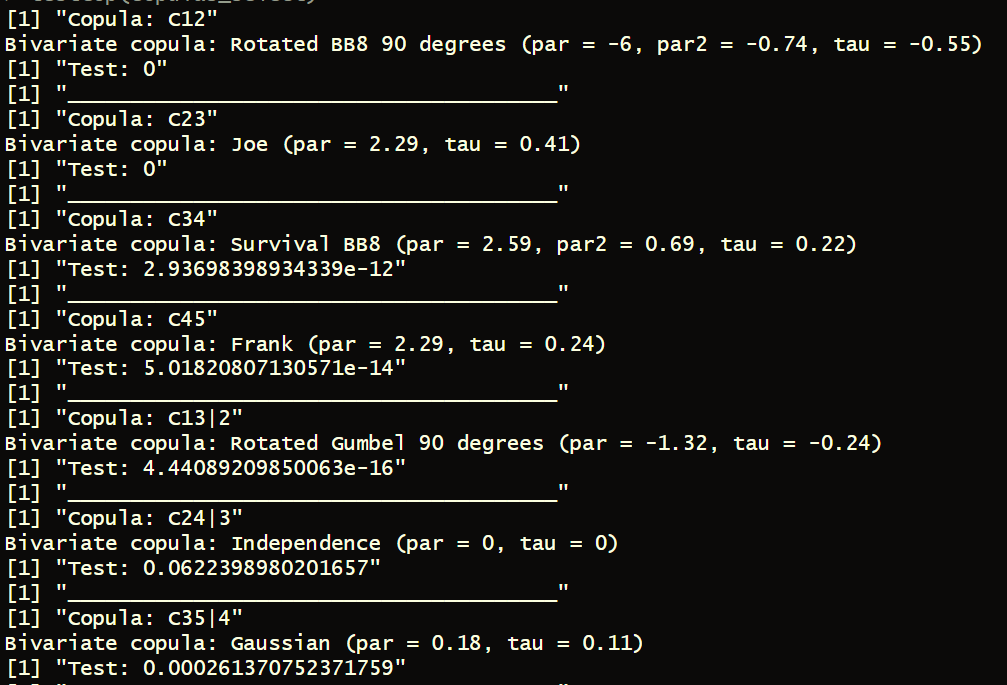
\includegraphics[width=0.46\textwidth]{4img/testH1.png}}
  \subfloat[Parte 2]{
   \label{ajusteHo2}
    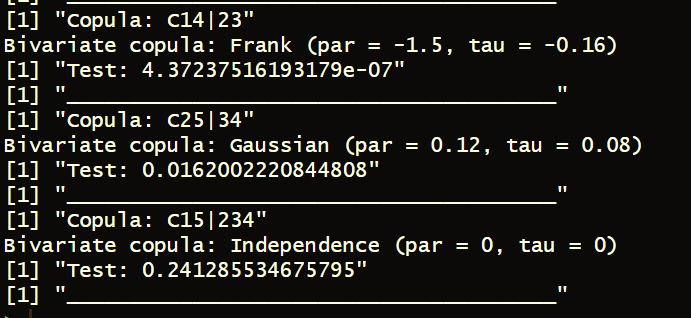
\includegraphics[width=0.46\textwidth]{4img/testH2.png}}
    \caption{Cópulas ajustadas la base de hombres.}
    \label{fig:copulasTestHo}
\end{figure}
\vspace{-0.3cm}

En cuanto a los tests de independencia de las cópulas ajustadas a los datos provenientes de hombres, ver Figura \ref{fig:copulasTestHo}, se observan $p-valores$ relativamente altos en los tests de independencia para las cópulas $C_{24|3}$ y $C_{15|234}$. Al igual que en el caso de la Figura \ref{fig:copulasTestMu}, esto sugiere que reducir una variable en estos niveles podría ser beneficioso para mejorar la capacidad del modelo para capturar las relaciones entre las covariables. 

\begin{figure}[H]
 \centering
  \subfloat[Parte 1]{
   \label{ajusteTo1}
    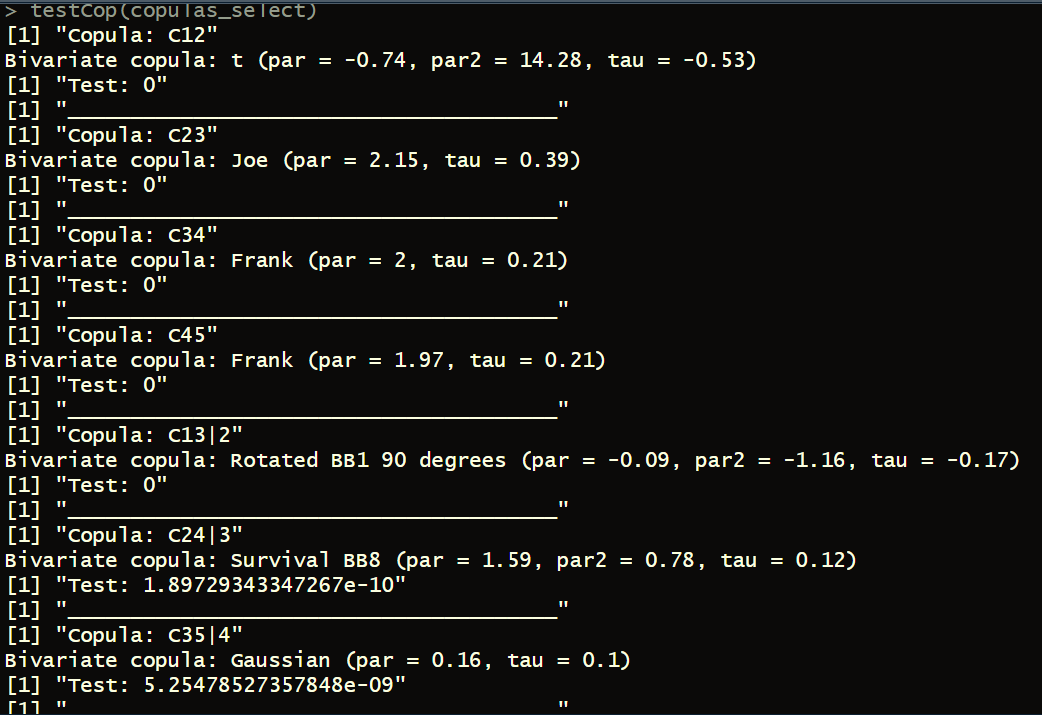
\includegraphics[width=0.46\textwidth]{4img/testT1.png}}
  \subfloat[Parte 2]{
   \label{ajusteTo2}
    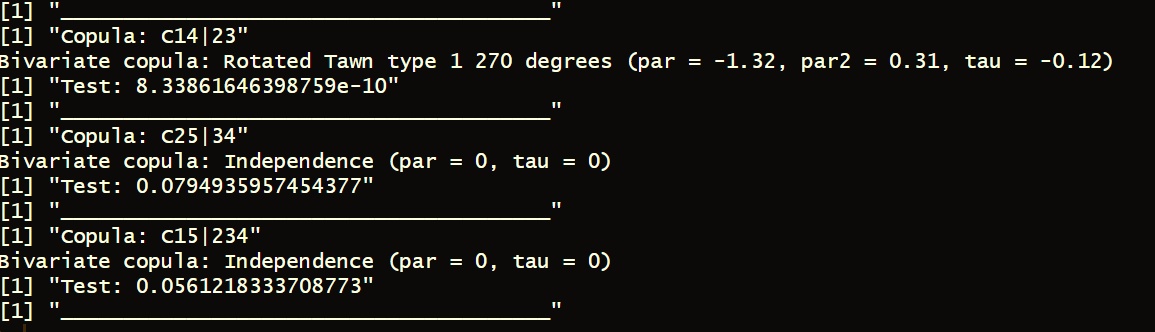
\includegraphics[width=0.46\textwidth]{4img/testT2.png}}
    \caption{Cópulas ajustadas la base de hombre y mujeres.}
    \label{fig:copulasTestTotal}
\end{figure}
\vspace{-0.3cm}

Por último, en la Figura \ref{fig:copulasTestTotal}
, se muestran las cópulas ajustadas para todo el conjunto de datos. La única cópula cuyo $p-valor$ para el test de independencia supera el nivel de confianza de $\alpha = 0.05$ es $C_{15|234}$. Es posible que esta diferencia, de solo tener una cópula independiente, se deba a que la cantidad de datos en este modelo es mayor. Al tener más datos, el modelo tiene una mayor capacidad para capturar la complejidad de las relaciones entre las variables, lo que puede resultar en una menor dependencia observada entre ellas.



%%%%%%%%%%%%%%%%%%%%%%%%%%%%%%%%%%%%%%%%%%%%%%%%%%%%%%%%%%%
%%%%%%%%%%%%% RESULTADOS DE VERDAD %%%%%%%%%%%%%%%%
%%%%%%%%%%%%%%%%%%%%%%%%%%%%%%%%%%%%%%%%%%%%%%%%%%%%%%%%%%%

\begin{landscape}

\subsection{Visualización del Modelo ajustado para Mujeres y hombres}
\begin{figure}[H]
    \centering
    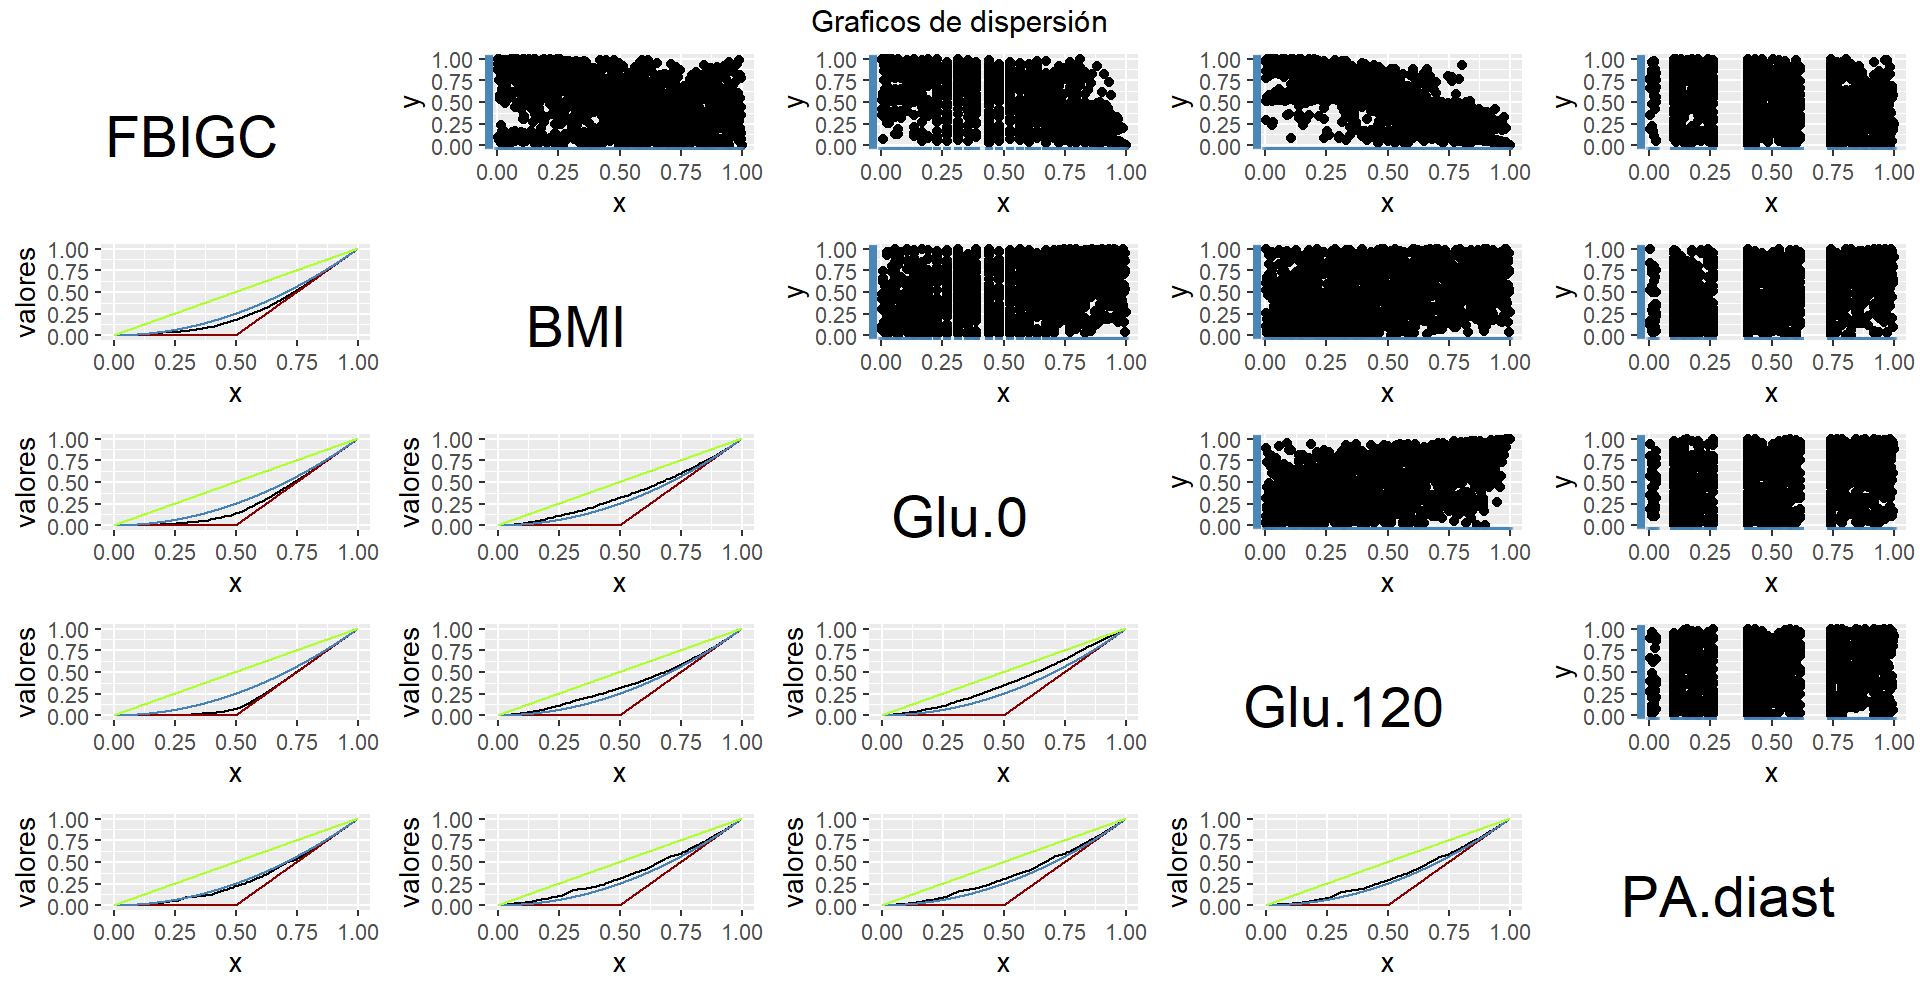
\includegraphics[height = 13.5 cm, width = 1.4 \textwidth]{4img/UdiagT.png}
    \caption{Diagonales y gráficos de dispersión en escala $u$ de hombres y mujeres.}
    \label{fig:diagTot}
\end{figure}

\end{landscape}

Uno de los aspectos más destacados de la Figura \ref{fig:diagTot}, es la posición de la diagonal de la cópula empírica en relación con la diagonal de cópula producto. En su mayor parte, la diagonal de la cópula empírica se sitúa por debajo o por encima de la diagonal, lo que indica que las dependencias entre las variables son mayoritariamente concordantes negativas o positivas, respectivamente. Este patrón de comportamiento es crucial, ya que las cópulas paramétricas pueden modelar estas relaciones de manera efectiva. Por lo tanto, como ya se había mencionado antes utilizar un modelo \texttt{R} vine con un ajuste paramétrico parece ser una estrategia apropiada.

Otro aspecto destacable es la partición que genera la variable presión diastólica. Recuérdese que esta es la presión arterial mínima registrada en las arterias durante el ciclo cardíaco cuando el corazón se encuentra en reposo entre latidos. La creación de estos tres grupos podría deberse a la presencia de tres subpoblaciones, como personas con presión diastólica normal, con hipertensión leve y con hipertensión moderada o grave o también podría provenir de las características de los instrumentos de medición. Sin embargo, no parece haber una dependencia estable con las otras variables.


Ahora, se muestran los heatmaps $\mathscr{H}\rho$, $\mathscr{H}\sigma$ y $\mathscr{H}$ de todas las cópulas utilizadas en el modelo D-vine para el modelo considerando hombre y mujeres. 


\begin{figure}[H]
 \centering
  \subfloat[$\mathscr{H}\rho_{C_{12}}$]{
   \label{C12rhoT}
    \includegraphics[width=0.3\textwidth]{4img/TotalrhoC12.png}}
  \subfloat[$\mathscr{H}\sigma_{C_{12}}$]{
   \label{C12sigmaT}
    \includegraphics[width=0.3\textwidth]{4img/TotalsigmaC12.png}}
  \subfloat[$\mathscr{H}_{C_{12}}$]{
   \label{C12HT}
    \includegraphics[width=0.3\textwidth]{4img/TotalHC12.png}}
\end{figure}

\begin{figure}[H]
 \centering
  \subfloat[$\mathscr{H}\rho_{C_{23}}$]{
   \label{C23rhoT}
    \includegraphics[width=0.3\textwidth]{4img/TotalrhoC23.png}}
  \subfloat[$\mathscr{H}\sigma_{C_{23}}$]{
   \label{C23sigmaT}
    \includegraphics[width=0.3\textwidth]{4img/TotalsigmaC23.png}}
  \subfloat[$\mathscr{H}_{C_{23}}$]{
   \label{C23HT}
    \includegraphics[width=0.3\textwidth]{4img/TotalHC23.png}}
\end{figure}

\begin{figure}[H]
 \centering
  \subfloat[$\mathscr{H}\rho_{C_{34}}$]{
   \label{C34rhoT}
    \includegraphics[width=0.3\textwidth]{4img/TotalrhoC34.png}}
  \subfloat[$\mathscr{H}\sigma_{C_{34}}$]{
   \label{C34sigmaT}
    \includegraphics[width=0.3\textwidth]{4img/TotalsigmaC34.png}}
  \subfloat[$\mathscr{H}_{C_{34}}$]{
   \label{C34HT}
    \includegraphics[width=0.3\textwidth]{4img/TotalHC34.png}}
\end{figure}

\begin{figure}[H]
 \centering
  \subfloat[$\mathscr{H}\rho_{C_{45}}$]{
   \label{C45rhoT}
    \includegraphics[width=0.3\textwidth]{4img/TotalrhoC45.png}}
  \subfloat[$\mathscr{H}\sigma_{C_{45}}$]{
   \label{C45sigmaT}
    \includegraphics[width=0.3\textwidth]{4img/TotalsigmaC45.png}}
  \subfloat[$\mathscr{H}_{C_{45}}$]{
   \label{C45HT}
    \includegraphics[width=0.3\textwidth]{4img/TotalHC45.png}}
    \caption{Cópulas ajustadas para mujeres y hombres, nivel $1$.}
    \label{fig:Modelo4TotalNivel1}
\end{figure}

Estas gráficas proporcionan una mejor comprensión del tipo y la fuerza de dependencia de cada cópula, y nos permitirá verificar visualmente la monotonicidad de la función para juzgar si el enfoque paramétrico es correcto. Estos heatmaps ayudan a identificar patrones de dependencia y a evaluar la idoneidad del modelo para capturar las relaciones entre las variables.

En la Figura \ref{fig:Modelo4TotalNivel1}, se muestran los heatmaps para cada cópula del nivel $1$. En la cópula $C_{12}$, que modela la relación entre $FBIGC$ y la glucosa al tiempo $120$. No se observa una clara dependencia en la primera parte del dominio, pero posteriormente se evidencia una dependencia de cuadrante negativo. Por otro lado, en la cópula $C_{23}$, que representa la relación entre la glucosa al tiempo $120$ y la glucosa al tiempo $0$, se observa una dependencia de cuadrante positivo que se presenta en todo el dominio. Además, en la cópula $C_{34}$, correspondiente a la glucosa al tiempo $0$ y el Índice de Masa Corporal, se observa una fuerte dependencia de cuadrante positivo.

En cuanto a la cópula $C_{45}$, se observa una relación singular caracterizada por líneas horizontales, que coinciden con los patrones de dispersión vistos en la Figura \ref{fig:diagTot}. Sin embargo, su dependencia fluctúa de positiva a negativa repentinamente, pero su depedencia en las zonas positivas no parece ser muy relevante. Es posible que sea adecuado intentar modelar esta cópula de manera no paramétrica para obtener un modelo más preciso y capturar mejor la complejidad de la relación entre las variables.

%%%%%%%%%%%%%%%%%%%%%%%%%%%%%%%%%%%%%%%%%%%%%%%%

\begin{figure}[H]
 \centering
  \subfloat[$\mathscr{H}\rho_{C_{13|2}}$]{
   \label{C13.2rhoT}
    \includegraphics[width=0.33\textwidth]{4img/TotalrhoC13.2.png}}
  \subfloat[$\mathscr{H}\sigma_{C_{13|2}}$]{
   \label{C13.2sigmaT}
    \includegraphics[width=0.33\textwidth]{4img/TotalsigmaC13.2.png}}
  \subfloat[$\mathscr{H}_{C_{13|2}}$]{
   \label{C13.2HT}
    \includegraphics[width=0.33\textwidth]{4img/TotalHC13.2.png}}
\end{figure}

\begin{figure}[H]
 \centering
  \subfloat[$\mathscr{H}\rho_{C_{24|3}}$]{
   \label{C24.3rhoT}
    \includegraphics[width=0.33\textwidth]{4img/TotalrhoC24.3.png}}
  \subfloat[$\mathscr{H}\sigma_{C_{24|3}}$]{
   \label{C24.3sigmaT}
    \includegraphics[width=0.33\textwidth]{4img/TotalsigmaC24.3.png}}
  \subfloat[$\mathscr{H}_{C_{24|3}}$]{
   \label{C24.3HT}
    \includegraphics[width=0.33\textwidth]{4img/TotalHC24.3.png}}
\end{figure}

\begin{figure}[H]
 \centering
  \subfloat[$\mathscr{H}\rho_{C_{35|4}}$]{
   \label{C35.4rhoT}
    \includegraphics[width=0.33\textwidth]{4img/TotalrhoC35.4.png}}
  \subfloat[$\mathscr{H}\sigma_{C_{35|4}}$]{
   \label{C35.4sigmaT}
    \includegraphics[width=0.33\textwidth]{4img/TotalsigmaC35.4.png}}
  \subfloat[$\mathscr{H}_{C_{35|4}}$]{
   \label{C35.4HT}
    \includegraphics[width=0.33\textwidth]{4img/TotalHC35.4.png}}
    \caption{Cópulas ajustadas para mujeres y hombres, nivel $2$.}
    \label{fig:Modelo4TotalNivel2}
\end{figure}

En la Figura \ref{fig:Modelo4TotalNivel2} se muestran las cópulas del nivel $2$. La primera cópula, $C_{13|2}$, corresponde a la variable respuesta y la medición de glucosa al tiempo $0$ condicionada a la glucosa al tiempo $120$. Se observa una relación de dependencia de cuadrante negativo, lo cual tiene sentido porque cuanto más baja es la variable respuesta, es posible que el cuerpo tenga dificultades para procesar el azúcar, lo que puede resultar en niveles altos de glucosa. Esta relación sugiere una posible asociación entre la variable respuesta y los niveles de glucosa al tiempo $0$ condicionados por los niveles de glucosa al tiempo 120, lo cual es coherente con el conocimiento médico sobre la fisiología del metabolismo del azúcar en el cuerpo.

La cópula $C_{24|3}$, que representa la relación entre la medición de glucosa al tiempo $120$ y el índice de masa corporal condicionado a los niveles de glucosa al tiempo $0$, muestra una relación de dependencia de cuadrante positiva, lo cual tiene sentido desde un punto de vista médico. Esto sugiere que a medida que los niveles de glucosa al tiempo $120$ aumentan, también tiende a aumentar el índice de masa corporal.

La relación entre la glucosa al tiempo $0$ y la presión diastólica, condicionada al índice de masa corporal, corresponde a la cópula $C_{35|4}$. Al observar una dependencia de cuadrante positiva, se esperaría que un aumento en los niveles de glucosa al tiempo $0$ esté asociado con una disminución en los valores de presión diastólica. Sin embargo, es importante ser cauteloso al interpretar esta relación, ya que puede estar influida por la distribución singular que se observó en la cópula $C_{45}$.

%%%%%%%%%%%%%%%%%%%%%%%%%%%%%%%%%%%%%%%%%%%%%%%%%%

\begin{figure}[H]
 \centering
  \subfloat[$\mathscr{H}\rho_{C_{14|23}}$]{
   \label{C14.23rhoT}
    \includegraphics[width=0.3\textwidth]{4img/TotalrhoC14.23.png}}
  \subfloat[$\mathscr{H}\sigma_{C_{14|23}}$]{
   \label{C14.23sigmaT}
    \includegraphics[width=0.3\textwidth]{4img/TotalsigmaC14.23.png}}
  \subfloat[$\mathscr{H}_{C_{14|23}}$]{
   \label{C14.23HT}
    \includegraphics[width=0.3\textwidth]{4img/TotalHC14.23.png}}
\end{figure}

\begin{figure}[H]
 \centering
  \subfloat[$\mathscr{H}\rho_{C_{25|34}}$]{
   \label{C25.34rhoT}
    \includegraphics[width=0.3\textwidth]{4img/TotalrhoC25.34.png}}
  \subfloat[$\mathscr{H}\sigma_{C_{25|34}}$]{
   \label{C25.34sigmaT}
    \includegraphics[width=0.3\textwidth]{4img/HomsigmaC25.34.png}}
  \subfloat[$\mathscr{H}_{C_{25|34}}$]{
   \label{C25.34HT}
    \includegraphics[width=0.3\textwidth]{4img/TotalHC25.34.png}}
    \caption{Cópulas ajustadas para mujeres y hombres, nivel $3$.}
    \label{fig:Modelo4TotalNivel3}
\end{figure}


Las cópula de nivel $3$ se muestran en la Figura \ref{fig:Modelo4TotalNivel3}. La cópula $C_{14|23}$, que representa la relación entre la variable respuesta y el índice de masa corporal condicionado a los niveles de glucosa al tiempo $0$ y $120$, muestra una baja concordancia. Esta relación se observa como negativa, y cuando el índice de masa corporal es bajo, parece haber independencia. Por otro lado, la cópula $C_{25|34}$ muestra una dependencia muy baja, lo cual está respaldado por los tests de independencia, lo que sugiere que la variable $5$ podría ser potencialmente desechada.

%%%%%%%%%%%%%%%%%%%%%%%%%%%%%%%%%%%%%%%%%%%%%%%%%%


\begin{figure}[H]
 \centering
  \subfloat[$\mathscr{H}\rho_{C_{15|234}}$]{
   \label{C15.234rhoT}
    \includegraphics[width=0.3\textwidth]{4img/TotalrhoC15.234.png}}
  \subfloat[$\mathscr{H}\sigma_{C_{15|234}}$]{
   \label{C15.234sigmaT}
    \includegraphics[width=0.3\textwidth]{4img/TotalsigmaC15.234.png}}
  \subfloat[$\mathscr{H}_{C_{15|234}}$]{
   \label{C15.234HT}
    \includegraphics[width=0.3\textwidth]{4img/TotalHC15.234.png}}
    \caption{Cópulas ajustadas para mujeres y hombres, nivel $3$.}
    \label{fig:Modelo4TotalNivel4}
\end{figure}

Finalmente, en la Figura \ref{fig:Modelo4TotalNivel4} se muestra la cópula $C_{15|234}$ correspondiente al último nivel. Esta cópula representa la relación entre la variable respuesta y la presión arterial diastólica, condicionada a los niveles de glucosa en el tiempo $120$ y $0$, y el índice de masa corporal se observa una dependencia muy baja.

A continuación en la Figura \ref{fig:tabla4varTotal}, se muestra la tabla de probabilidades de tener resistencia a la insulina por clasificación de peso y glucosa para datos de hombres y mujeres. Para recordar la especificación de las clasificaciones se puede consultar las subsecciones \ref{ClasificaVar} y \ref{subTabla}.

%%%%%%%%%%%%%%%%%%%%%%%%%%%%%%%%%%%%%%%%%%%%%%%%%%%%%%%%%%%

\subsection{Tabla Resumen del Modelo}

La probabilidad de pertenecer a la clase de individuos saludables es muy alta para las personas con niveles de glucosa normales y un peso normal o con sobrepeso. En la categoría de personas con niveles de glucosa normales pero con obesidad, la probabilidad de tener resistencia a la insulina con predisfunción de las células beta aumenta. A partir de esta categoría, la probabilidad de tener resistencia a la insulina con estrés de las células beta aumenta, siendo esta la predominante en todas las clasificaciones con niveles de glucosa prediabéticos. Las categorías cuyos niveles de glucosa son diabéticos ya son clasificadas como pacientes con resistencia a la insulina con disfunción de las células beta.


\begin{figure}[H]

    \centering
    \includegraphics[height = 12 cm, width = 0.99 \textwidth]{4img/tablaT.png}
    \caption{Tabla de probabilidades de cada Clase.}
    \label{fig:tabla4varTotal}
\end{figure}



Las ventajas de tener este tipo de representaciones, y no solo quedarse con el modelo computacional, son significativas. Estas representaciones pueden llevarse a todo tipo de comunidades, incluidas aquellas con escasos recursos. Al proporcionar una visualización clara y accesible, se facilita la comprensión y el análisis de los datos sin necesidad de equipos o software avanzado. Esto es especialmente importante en áreas donde el acceso a tecnología de punta es limitado, permitiendo a los profesionales de la salud y a los encargados de la toma de decisiones identificar patrones y tomar medidas preventivas de manera más efectiva.

%%%%%%%%%%%%%%%%%%%%%%%%%%%%%%%%%%%%%%%%%%%%%%%%%%%%%%%%%
%%%%%%%  G R A F I C O S  D E  E F E C T O S  %%%%%%%%%%%
%%%%%%%%%%%%%%%%%%%%%%%%%%%%%%%%%%%%%%%%%%%%%%%%%%%%%%%%%

\subsection{Comparación de Modelos}

Con el objetivo de comparar las diferencias entre los ajustes de cada subconjunto de datos, se utilizará la gráfica de efectos para visualizar el impacto que tiene cada covariable sobre la variable respuesta. Además, se emplearán las curvas de nivel para comparar cómo son las cópulas ajustadas para cada par de variables, tanto no condicionadas como condicionadas. Estas herramientas nos permitirán evaluar de manera detallada cómo se relacionan las variables en diferentes contextos y subgrupos de datos, lo que facilitará la identificación de patrones y relaciones importantes en el modelo.

En las gráficas de efectos de la variable glucosa al tiempo $120$ se muestra en las Figuras \ref{Efec120M4}, \ref{Efec120H4} y \ref{Efec120T4}, se observa que el efecto difiere según el género. En el caso de las mujeres, esta variable influye principalmente en sus valores bajos, teniendo un efecto similar para valores mayores a $120$ $mg/dl$. Por otro lado, en los hombres, parece que la respuesta cambia poco para valores menores a aproximadamente $100$ $mg/dl$. Luego, influye significativamente en el cambio de la respuesta hasta valores menores a $300$ $mg/dl$, y vuelve a cambiar poco para valores mayores a este umbral. Estas diferencias en el efecto de la variable glucosa al tiempo $120$ entre géneros son importantes y pueden tener implicaciones significativas en el análisis y la interpretación de los resultados del modelo.

En el modelo combinado de hombres y mujeres, se observa una combinación de ambas tendencias. La gráfica muestra una tendencia descendente, similar al modelo de las mujeres, pero no tiene una forma sigmoidal tan pronunciada como la de los hombres. Sin embargo, tampoco se estanca, lo que sugiere que hay una influencia continua de la variable en la respuesta a lo largo de su rango de valores. Esta combinación de tendencias refleja la complejidad de la relación entre la variable en cuestión y la respuesta, que puede variar según el género y otros factores.

\begin{figure}[H]
 \centering
  \subfloat[Glu.120, Mujeres]{
   \label{Efec120M4}
    \includegraphics[width=0.3\textwidth]{4img/MujGlu.120Efec.png}}
  \subfloat[Glu.120, Hombres]{
   \label{Efec120H4}
    \includegraphics[width=0.3\textwidth]{4img/HomGlu.120Efec.png}}
  \subfloat[Glu.120, Total]{
   \label{Efec120T4}
    \includegraphics[width=0.3\textwidth]{4img/TotalGlu.120Efec.png}}
\end{figure}

\begin{figure}[H]
 \centering
  \subfloat[Glu.0, Mujeres]{
   \label{Efec0M4}
    \includegraphics[width=0.3\textwidth]{4img/MujGlu.0Efec.png}}
  \subfloat[Glu.0, Hombres]{
   \label{Efec0H4}
    \includegraphics[width=0.3\textwidth]{4img/HomGlu.0Efec.png}}
  \subfloat[Glu.0, Total]{
   \label{Efec0T4}
    \includegraphics[width=0.3\textwidth]{4img/TotalGlu.0Efec.png}}
\end{figure}

\begin{figure}[H]
 \centering
  \subfloat[BMI, Total]{
   \label{EfecBMIM4}
    \includegraphics[width=0.3\textwidth]{4img/MujBMIEfec.png}}
  \subfloat[BMI, Total]{
   \label{EfecBMIH4}
    \includegraphics[width=0.3\textwidth]{4img/HomBMIEfec.png}}
  \subfloat[BMI, Total]{
   \label{EfecBMIT4}
    \includegraphics[width=0.3\textwidth]{4img/TotalBMIEfec.png}}
\end{figure}

\begin{figure}[H]
 \centering
  \subfloat[PA.diast, Mujeres]{
   \label{EfecPAM4}
    \includegraphics[width=0.3\textwidth]{4img/MujPA.diastEfec.png}}
  \subfloat[PA.diast, Hombres]{
   \label{EfecPAH4}
    \includegraphics[width=0.3\textwidth]{4img/HomPA.diastEfec.png}}
  \subfloat[PA.diast, Total]{
   \label{EfecPAT4}
    \includegraphics[width=0.3\textwidth]{4img/TotalPA.diastEfec.png}}
    \caption{Gráficas de efectos para la regresión de 4 variables.}
    \label{fig:efecto4}
\end{figure}



Ahora se analizará los efectos de la glucosa en tiempo $0$, Figuras \ref{Efec0M4}, \ref{Efec0H4} y \ref{Efec0T4} . En mujeres se observa que inicialmente influye levemente en la variable respuesta. Luego, este efecto aumenta y posteriormente disminuye. Sin embargo, el nivel de aumento o disminución depende en gran medida del cuantil que se considere. Por otro lado, en hombres, el decrecimento en la variable respuesta es muy drástico al principio, y luego se vuelve muy leve. Al igual que en mujeres, este nivel de cambio también se ve afectado por el nivel del cuantil con el que se realice la regresión. Estas diferencias en los efectos de la glucosa en tiempo $0$ entre géneros resaltan la importancia de considerar las características específicas de cada grupo al analizar los datos y desarrollar modelos predictivos.


En el efecto de la variable $Glu.0$ del modelo combinado de hombres y mujeres, parece haber un cambio en todos los valores de la glucosa, y estos cambios varían de acuerdo al nivel de la regresión. Sin embargo, es importante destacar que el rango de la variable respuesta en este modelo combinado es más grande que los rangos individuales de hombres y mujeres. Esto sugiere que la inclusión de ambos géneros puede resultar en una variabilidad más amplia en la variable respuesta, lo que podría reflejar la diversidad de respuestas dentro de la población en general. 

En las Figuras \ref{EfecPAM4}, \ref{EfecPAH4} y \ref{EfecPAT4}, se pueden observar los efectos de la variable presión diastólica sobre la variable respuesta. Se puede notar que no hay un cambio significativo en la variable respuesta ante los diferentes valores de la presión diastólica en los $3$ modelos. Esto indica que la presión diastólica no aporta información relevante al modelo, ya que su contribución es prácticamente nula en relación con la variable respuesta. Por lo tanto, se puede concluir que esta variable no tiene un impacto significativo y podría ser excluida del modelo sin perder precisión predictiva.

Los efectos de las variables $BMI$ aparecen en las Figuras \ref{EfecBMIM4}, \ref{EfecBMIH4} y \ref{EfecBMIT4}. Las interpretaciones son similares a los casos de las variables $Glu.0$ y $Glu.120$, por lo que no se describen. 

En el Apéndice \ref{ApendiceA}, se presentan las visualizaciones de los modelos D-vine ajustados específicamente para mujeres y para hombres, junto con sus respectivas tablas de probabilidades. La inclusión de estos modelos en el apéndice permite una evaluación detallada y comparativa de las diferencias y similitudes en la dependencia entre variables según el género, sin interrumpir el flujo principal del análisis en el cuerpo del documento.
\cleardoublepage

\chapter{Conclusiones}

La Diabetes Mellitus representa un desafío a nivel mundial, siendo la cuarta principal causa de muerte durante el $2023$ y la segunda en México \cite{INEGI}. A pesar de que se han propuesto diversos modelos matemáticos para comprender esta enfermedad, una de las mayores dificultades en su manejo efectivo radica en la falta de modelos precisos y adaptados a poblaciones específicas. Este trabajo propone un modelo ajustado especialmente para la población mexicana, con el objetivo de abordar esta brecha y ofrecer una herramienta que pueda ser utilizada en cualquier tipo de comunidad.

El problema planteado se abordó primero desde la parte biológica, pues es esencial comprender el proceso de la homeostasis de la glucosa para extraer los factores clave que regulan los niveles de glucosa en la sangre y el origen de los síndromes metabólicos. Además, se hizo un breve recorrido sobre los modelos matemáticos anteriormente propuestos para esta enfermedad, evaluando sus fortalezas y limitaciones.

Con las curvas de información de niveles de glucosa e insulina de alrededor de $1500$ individuos de la prueba oral de tolerancia a la glucosa, provenientes de la población mexicana proporcionadas por la Dra. Adriana Monroy, se propuso emplear la técnica de las bandas de profundidad junto con una medida para la efectiva de la sensibilidad a la insulina. Esta técnica y medida permite crear una variable respuesta escalar que conserva su esencia funcional, idea desarrollada por el estudiante de doctorado de CIMAT, Israel Emmanuel Ambriz Lobato, en su trabajo de tesis. Haciendo uso de regresión cuantil, esta técnica permite realizar la regresión con un cierto nivel de confianza, además tiene varias ventajas, siendo una de las más destacables su robustez ante la presencia de valores atípicos.

Como herramienta final, se propuso hacer el ajuste utilizando un modelo de cópulas llamado D-Vine. La idea fundamental es la descomposición de la función de distribución de un vector en cópulas bivariadas, las cuales se determinan con un grafo o árboles. Utilizando el grafo, es sencillo visualizar las dependencias condicionales o cópulas. Esto se implementó haciendo uso del paquete \textbf{VineCopula} y varias técnicas de visualización de medidas de dependencia para realizar análisis exploratorio.

Después de ajustar los dos modelos de regresión con $3$ y $4$ variables, gracias a todas las herramientas de visualización implementadas y la significancia de los test de independencia, fue sencillo poder distinguir la importancia de las variables en el modelo y así decidir si desecharlas o no. Además, la visualización de las curvas de nivel de cada cópula fue otra herramienta útil, ya que permitió observar y comparar cómo son las interacciones de todas las variables hasta las condicionales, estas fueron implementadas en el paquete. Estas curvas de nivel nos brindan una representación gráfica de la estructura de dependencia entre las variables, lo que facilita la identificación de patrones y relaciones complejas que pueden no ser evidentes al analizar los datos de forma individual.

Adicionalmente, se han computado gráficos de efectos para visualizar la variabilidad y la relación entre la variable respuesta y su impacto en la predicción de la diabetes. Estos gráficos han demostrado ser fundamentales para identificar patrones y tendencias, así como para resaltar variables que no aportan información significativa al modelo. Esta capacidad de visualización facilita la selección de variables relevantes y mejora la interpretabilidad y precisión de los resultados.

En conclusión, el modelo propuesto no solo busca mejorar la comprensión y el manejo de la diabetes en la población mexicana, sino también proporcionar una herramienta accesible y aplicable a comunidades con recursos limitados. Al ofrecer un modelo simplificado y visualmente intuitivo, se espera que profesionales de la salud puedan tomar decisiones más informadas y efectivas en la lucha contra esta enfermedad.

Como trabajo a futuro, se podría seguir experimentando con otras variables y culminar con alguna aplicación de fácil uso en los hospitales. Por otro lado, en la parte computacional, se planea continuar con el desarrollo de la paquetería que implementa las herramientas gráficas para modelos D-vine y poder implementar más modalidades a las cópulas. Actualmente, el modelo construido solo utiliza cópulas paramétricas. Sin embargo, se busca permitir que el usuario pueda asignar una cópula paramétrica, no paramétrica, o una combinación específica de cópulas, ofreciendo así mayor flexibilidad y precisión en el ajuste del modelo. 

Además, se planea liberar esta paquetería en CRAN. El proyecto ya se encuentra implementado en GitHub, en el siguiente repositorio \url{https://github.com/BesitosDeBaba/deerVineReg/tree/master}. Sin embargo, se tiene previsto extender el proyecto implementando cópulas no paramétricas y combinándolas en el ajuste, así como mejorar la función cuantil. Esto permitirá que la herramienta esté disponible al público en general, facilitando su uso y adopción por parte de la comunidad científica y médica.
\cleardoublepage

%%%%%%%%%%%%%%%%%%%%%%%%%%%%%%%%%%%%%%%%%%%%%%%%%%
%%%%%%%%%%%%%%%%%%%%%%%%%%%%%%%%%%%%%%%%%%%%%%%%%%
%%% Referencias
\printbibliography[title={Referencias Bibliográficas}, heading=bibintoc]
\cleardoublepage

%%%%%%%%%%%%%%%%%%%%%%%%%%%%%%%%%%%%%%%%%%%%%%%%%%
%%%%%%%%%%%%%%% A P E N D I C E %%%%%%%%%%%%%%%%%%
\appendix

\chapter{Comparaciones por Género}\label{ApendiceA}

En este apéndice se presentan los resultados de los otros modelos discutidos en esta tesis, que no se abordaron con detalle en el Capítulo 4. Aquí se encontrarán los análisis exploratorios del modelo ajustado para hombres y del modelo ajustado para mujeres, junto con sus respectivas interpretaciones. Además, se incluyen las comparaciones finales entre ambos modelos. Esta información adicional proporciona una comprensión más profunda de las diferencias y similitudes en las relaciones entre variables según el género, permitiendo una evaluación más completa y matizada de los resultados.

%%%%%%%%%%%%%%%%%%%%%%%%%%%%%%%%%%%%%%%%%%%%%%%%%%%%%%
%%%%%%% A N A L I S I S  P O R  G E N E R O %%%%%%%%%%
%%%%%%%%%%%%%%%%%%%%%%%%%%%%%%%%%%%%%%%%%%%%%%%%%%%%%%

\section{Boxplot Funcionales por Género}

Antes de comenzar el análisis de los modelos ajustados, se realizaron boxplots funcionales para comparar las diferencias en el comportamiento de las curvas de glucosa e insulina por género en cada prediagnóstico. Este análisis preliminar tiene como objetivo comprender mejor la naturaleza del procesamiento de glucosa en los diferentes géneros, proporcionando una base sólida para interpretar los modelos ajustados posteriormente.

En la Figura \ref{fig:glucosaNormal}, se muestra una comparación de los boxplots funcionales entre hombres y mujeres de individuos cuyo prediagnóstico es normal. En la curva mediana de ambos boxplots, se observa una tendencia creciente seguida de un descenso. Sin embargo, en la curva mediana asociada a hombres, el pico se alcanza a los $30$ minutos y luego desciende, mientras que en las mujeres, el pico parece estar entre los $30$ y $60$ minutos antes de descender. Este comportamiento también se observa en la curva del tercer cuartil. Este comportamiento coincide con hallazgos de estudios previos que comparan la homeostasis entre hombres y mujeres, donde se concluye que las mujeres suelen mostrar niveles más bajos de glucosa al inicio de la prueba oral de tolerancia a la glucosa y terminan con niveles más altos \cite{GenderDifferences2018}.

Adicionalmente, en las curvas asociadas al primer cuartil en ambos casos, se observa un descenso seguido de un ascenso, lo que sugiere posibles errores de medición.


\begin{figure}[H]
 \centering
  \subfloat[Mujeres]{
   \label{bfMuGluNormal}
    \includegraphics[width=0.45\textwidth]{img/bfMujgluNormal.png}}
  \subfloat[Hombres]{
   \label{bfHoGluNormal}
    \includegraphics[width=0.45\textwidth]{img/bfHogluNormal.png}}
    \caption{Boxplot funcional para las curvas de glucosa para personas con prediagnóstico normal.}
    \label{fig:glucosaNormal}
\end{figure}

Los boxplots correspondientes a las curvas de insulina de la Figura \ref{fig:insulinaNormal}, muestran un comportamiento similar en ambos géneros, con una curva mediana ascendente seguida de un descenso, aunque en el caso de los hombres esta curva parece ser más pronunciada.

Es importante destacar que en el boxplot correspondiente a mujeres se observan varios outliers, con niveles de insulina bastante altos. Esto sugiere la posibilidad de que estos individuos estén experimentando resistencia a la insulina, aunque esta condición aún no se refleje claramente en su curva de insulina. Por otro lado, la curva del primer cuartil muestra niveles bajos en ambos casos.

En cuanto al tercer cuartil, la curva de las mujeres se asemeja bastante a la curva correspondiente a la mediana, lo que sugiere una forma común. Sin embargo, en los hombres esta curva se modifica ligeramente posiblemente algún error de medición. 

De acuerdo, con el articulo `\textit{Gender Differences in Glucose Homeostasis and Diabetes}' \cite{GenderDifferences2018} las mujeres, en comparación con los hombres de la misma edad, tienden a tener menor masa muscular esquelética y mayor masa de tejido adiposo, así como mayores niveles circulantes de ácidos grasos libres (FFA) y un contenido lipídico intramiocelular elevado. Estos factores podrían promover la resistencia a la insulina en las mujeres. A pesar de estas diferencias, las mujeres son tan sensibles a la insulina como los hombres.


\begin{figure}[H]
 \centering
  \subfloat[Mujeres]{
   \label{bfMuGluInsulina}
    \includegraphics[width=0.45\textwidth]{img/bfMuInsNormal.png}}
  \subfloat[Hombres]{
   \label{bfHoGluInsulina}
    \includegraphics[width=0.45\textwidth]{img/bfHoInsNormal.png}}
    \caption{Boxplot funcional para las curvas de insulina para personas con prediagnóstico normal.}
    \label{fig:insulinaNormal}
\end{figure}


%%%%%%%%%%%%%%%%%%%%%%%%%%%%%%%%%%%%%%%%%%%%%%%%%%%%%%%%

En la categoría de prediabéticos, los boxplots funcionales de glucosa para hombres y mujeres muestran diferencias significativas. La curva mediana en mujeres es ascendente hasta el minuto $90$ y luego comienza a descender, mientras que en hombres alcanza su máximo a los $60$ minutos. El tercer cuartil presenta un comportamiento similar, aunque en mujeres parece haber una mayor resistencia a la insulina, ya que los valores de glucosa no disminuyen tanto.

La curva del primer cuartil correspondientes a hombres y mujeres muestra nuevamente un patrón ascendente, descendente y posteriormente ascendente, lo que podría sugerir otro posible error de medición. Por otro lado, la curva del bigote inferior de mujeres parece seguir la misma forma que la curva mediana de mujeres, lo que sugiere una tendencia común en este grupo.

Adicionalmente, a los $120$ minutos, los valores de las curvas de glucosa de las mujeres tienen una varianza mucho mayor que los de los hombres. 

La prevalencia de síndromes pre-diabéticos, como la glucosa en ayuno alterada (IFG) y la tolerancia alterada a la glucosa (IGT) que corresonden a niveles de glucosa a las dos horas entre $140$ y $199$, también presenta un sesgo sexual \cite{GenderDifferences2018}. Específicamente, la IFG es más prevalente en los hombres, mientras que la IGT es más común en las mujeres. Estas diferencias destacan la importancia de considerar el sexo como un factor en el diagnóstico y tratamiento de condiciones pre-diabéticas, ya que hombres y mujeres pueden presentar distintos riesgos y necesidades en el manejo de su salud metabólica \cite{GenderDifferences2018}.

\begin{figure}[H]
 \centering
  \subfloat[Mujeres]{
   \label{bfMuGluPredia}
    \includegraphics[width=0.45\textwidth]{img/bfMugluPredia.png}}
  \subfloat[Hombres]{
   \label{bfHoGluPredia}
    \includegraphics[width=0.45\textwidth]{img/bfHogluPredia.png}}
    \caption{Boxplot funcional para las curvas de glucosa para personas con prediagnóstico prediabetes.}
    \label{fig:glucosaPredia}
\end{figure}


En la Figura \ref{fig:insulinaPredia}, se muestran los boxplots funcionales de las curvas de insulina de ambos géneros en individuos prediabéticos. Uno de los aspectos más destacables son los outliers, que en ambos casos presentan valores muy altos. Este comportamiento podría ser indicativo de individuos con una resistencia a la insulina significativa, que están al borde de desarrollar diabetes.

\begin{figure}[H]
 \centering
  \subfloat[Mujeres]{
   \label{bfMuInsPredia}
    \includegraphics[width=0.45\textwidth]{img/bfMuInsPredia.png}}
  \subfloat[Hombres]{
   \label{bfHoInsPredia}
    \includegraphics[width=0.45\textwidth]{img/bfHoInsPredia.png}}
    \caption{Boxplot funcional para las curvas de insulina para personas con prediagnóstico prediabetes.}
    \label{fig:insulinaPredia}
\end{figure}

En las mujeres, la curva mediana alcanza su máximo en el minuto 90, y el tercer cuartil se encuentra más separado de la mediana en comparación con el primer cuartil, lo que evidencia valores altos en los datos. Además, se aprecia una mayor varianza en los valores del minuto 120 en las mujeres en comparación con los hombres.


En los hombres, la curva mediana parece ser similar a la de las mujeres, pero los valores del tercer cuartil son ligeramente más bajos. Estos boxplots pueden resultar difíciles de discernir en cuanto a categorías, ya que la curva del primer cuartil es muy baja tanto en hombres como en mujeres, lo que podría indicar individuos con diabetes, y también se observan curvas muy altas.


%%%%%%%%%%%%%%%%%%%%%%%%%%%%%%%%%%%%%%%%%%%%%%%%%%

En la categoría diabética, en ambos boxplots funcionales las curvas medianas de glucosa se encuentran en un rango alto, alcanzando su máximo en el minuto $90$ para luego descender, ver Figura \ref{fig:glucosaDiabetes}. Sin embargo, en el caso de los hombres, la curva media desciende más rápidamente en comparación con las mujeres, donde parece ser más gradual. Es importante destacar que la varianza en el último instante es mayor en hombres, y se observa que el bigote superior alcanza niveles de alrededor de $600$.

\begin{figure}[H]
 \centering
  \subfloat[Mujeres]{
   \label{bfMuGluDia}
    \includegraphics[width=0.45\textwidth]{img/bfMugluDiab.png}}
  \subfloat[Hombres]{
   \label{bfHoGluDia}
    \includegraphics[width=0.45\textwidth]{img/bfHoGluDiabetes.png}}
    \caption{Boxplot funcional para las curvas de glucosa para personas con prediagnóstico diabetes.}
    \label{fig:glucosaDiabetes}
\end{figure}

Además, es notable que en esta categoría casi no hay outliers; en el boxplot de hombres no se presentan, y en el de mujeres hay dos, uno de los cuales muestra una caída muy abrupta en el minuto $30$, lo cual es biológicamente poco plausible y podría atribuirse a un error de medición. Similarmente, se observa una caída repentina en el bigote inferior de los hombres en el minuto $90$, lo que también podría ser atribuido a un error tipográfico.

En ambos casos parece haber un patrón discernible: en los hombres, el ascenso alcanza rangos más altos, mientras que en las mujeres parece ser un poco más suave. Sin embargo, sería difícil afirmar que esta diferencia es característica de cada género, ya que puede haber variabilidad individual significativa dentro de cada grupo.

La prevalencia de la diabetes tipo 2 también se caracteriza por una diferencia de sexo, de acuerdo a los resultados de los estudios realizados en \cite{GenderDifferences2018}. En general, la prevalencia global de diabetes es mayor en hombres, pero hay más mujeres con diabetes que hombres.

\begin{figure}[H]
 \centering
  \subfloat[Mujeres]{
   \label{bfMuInsDia}
    \includegraphics[width=0.45\textwidth]{img/bfMuInsDiabetes.png}}
  \subfloat[Hombres]{
   \label{bfHoInsDia}
    \includegraphics[width=0.45\textwidth]{img/bfHoInsDiabetes.png}}
    \caption{Boxplot funcional para las curvas de insulina para personas con prediagnóstico diabetes.}
    \label{fig:insulinaDiabetes}
\end{figure}

Los boxplots funcionales correspondientes a las curvas de insulina de la categoría diabética se muestran en la Figura \ref{fig:insulinaDiabetes}. Estos boxplots parecen presentar características significativas. La curva mediana correspondiente al grupo de hombres es más baja que la de mujeres. Por otro lado, las curvas asociadas al primer y tercer cuartil de la categoría de hombres están muy cercanas a la mediana, lo que indica poca variabilidad. En cambio, las curvas del primer y tercer cuartil de mujeres están más separadas, lo que indica mayor variabilidad.

Varias curvas representativas de ambos boxplots muestran el comportamiento inusual de subir, bajar y luego volver a subir. Aunque estos cambios pueden atribuirse a errores de medición, dado que no son extremadamente abruptos, no se descartarán. Los outliers son de escala, sin embargo, siguen este patrón de solo ascenso y en cantidades reducidas, lo cual concuerda con el perfil diabético.


%%%%%%%%%%%%%%%%%%%%%%%%%%%%%%%%%%%%%%%%%%%%%%%%%%%%%%%%%%%%%
%%%%%%%%%%%%%%%%%%%%%%%%%%%%%%%%%%%%%%%%%%%%%%%%%%%%%%%%%%%%%
%%%%%%%%%%%%%%%%%%%%%%%%%%%%%%%%%%%%%%%%%%%%%%%%%%%%%%%%%%%%%

\begin{landscape}
\subsection{Visualización del Modelo ajustado para Mujeres}

\begin{figure}[H]
    \centering
    \includegraphics[height = 13.5 cm, width = 1.4 \textwidth]{4img/UdiagM.png}
    \caption{Diagonales y gráficos de dispersión en escala $u$.}
    \label{fig:diagMU}
\end{figure}
\end{landscape}

En la Figura \ref{fig:diagMU}, se presentan las diagonales de las cópulas empíricas con respecto a las diagonales de cópulas de referencia, junto con los gráficos de dispersión de las variables de individuos del género masculino. Al igual que en el caso de hombres y mujeres, expuesto en el Capítulo \ref{Resultados}. En su mayor parte, la diagonal de la cópula empírica se encuentra por debajo o por encima de la diagonal, lo que indica que las dependencias entre las variables son mayoritariamente concordantes negativas o positivas, respectivamente. También se observa la misma partición generada por la variable de presión diastólica.


\begin{figure}[H]
 \centering
  \subfloat[$\mathscr{H}\rho_{C_{12}}$]{
   \label{C12rho}
    \includegraphics[width=0.33\textwidth]{4img/MujrhoC12.png}}
  \subfloat[$\mathscr{H}\sigma_{C_{12}}$]{
   \label{C12sigma}
    \includegraphics[width=0.33\textwidth]{4img/MujsigmaC12.png}}
  \subfloat[$\mathscr{H}_{C_{12}}$]{
   \label{C12H}
    \includegraphics[width=0.33\textwidth]{4img/MujHC12.png}}
\end{figure}

\begin{figure}[H]
 \centering
  \subfloat[$\mathscr{H}\rho_{C_{23}}$]{
   \label{C23rho}
    \includegraphics[width=0.33\textwidth]{4img/MujrhoC23.png}}
  \subfloat[$\mathscr{H}\sigma_{C_{23}}$]{
   \label{C23sigma}
    \includegraphics[width=0.33\textwidth]{4img/MujsigmaC23.png}}
  \subfloat[$\mathscr{H}_{C_{23}}$]{
   \label{C23H}
    \includegraphics[width=0.33\textwidth]{4img/MujHC23.png}}
\end{figure}

\begin{figure}[H]
 \centering
  \subfloat[$\mathscr{H}\rho_{C_{34}}$]{
   \label{C34rho}
    \includegraphics[width=0.33\textwidth]{4img/MujrhoC34.png}}
  \subfloat[$\mathscr{H}\sigma_{C_{34}}$]{
   \label{C34sigma}
    \includegraphics[width=0.33\textwidth]{4img/MujsigmaC34.png}}
  \subfloat[$\mathscr{H}_{C_{34}}$]{
   \label{C34H}
    \includegraphics[width=0.33\textwidth]{4img/MujHC34.png}}
\end{figure}

\begin{figure}[H]
 \centering
  \subfloat[$\mathscr{H}\rho_{C_{45}}$]{
   \label{C45rho}
    \includegraphics[width=0.33\textwidth]{4img/MujrhoC45.png}}
  \subfloat[$\mathscr{H}\sigma_{C_{45}}$]{
   \label{C45sigma}
    \includegraphics[width=0.33\textwidth]{4img/MujsigmaC45.png}}
  \subfloat[$\mathscr{H}_{C_{45}}$]{
   \label{C45H}
    \includegraphics[width=0.33\textwidth]{4img/MujHC45.png}}
    \caption{Cópulas ajustadas para Mujeres, nivel $1$.}
    \label{fig:Modelo4MujNivel1}
\end{figure}

%%%%%%%%%%%%%%%%%%%%%%%%%%%%%%%%%%%%%%%%%%%%%%%%%%

\begin{figure}[H]
 \centering
  \subfloat[$\mathscr{H}\rho_{C_{13|2}}$]{
   \label{C13.2rho}
    \includegraphics[width=0.33\textwidth]{4img/MujrhoC13.2.png}}
  \subfloat[$\mathscr{H}\sigma_{C_{13|2}}$]{
   \label{C13.2sigma}
    \includegraphics[width=0.33\textwidth]{4img/MujsigmaC13.2.png}}
  \subfloat[$\mathscr{H}_{C_{13|2}}$]{
   \label{C13.2H}
    \includegraphics[width=0.33\textwidth]{4img/MujHC13.2.png}}
\end{figure}

\begin{figure}[H]
 \centering
  \subfloat[$\mathscr{H}\rho_{C_{24|3}}$]{
   \label{C24.3rho}
    \includegraphics[width=0.33\textwidth]{4img/MujrhoC24.3.png}}
  \subfloat[$\mathscr{H}\sigma_{C_{24|3}}$]{
   \label{C24.3sigma}
    \includegraphics[width=0.33\textwidth]{4img/MujsigmaC24.3.png}}
  \subfloat[$\mathscr{H}_{C_{24|3}}$]{
   \label{C24.3H}
    \includegraphics[width=0.33\textwidth]{4img/MujHC24.3.png}}
\end{figure}

\begin{figure}[H]
 \centering
  \subfloat[$\mathscr{H}\rho_{C_{35|4}}$]{
   \label{C35.4rho}
    \includegraphics[width=0.33\textwidth]{4img/MujrhoC35.4.png}}
  \subfloat[$\mathscr{H}\sigma_{C_{35|4}}$]{
   \label{C35.4sigma}
    \includegraphics[width=0.33\textwidth]{4img/MujsigmaC35.4.png}}
  \subfloat[$\mathscr{H}_{C_{35|4}}$]{
   \label{C35.4H}
    \includegraphics[width=0.33\textwidth]{4img/MujHC35.4.png}}
    \caption{Cópulas ajustadas para Mujeres, nivel $2$.}
    \label{fig:Modelo4MujNivel2}
\end{figure}

%%%%%%%%%%%%%%%%%%%%%%%%%%%%%%%%%%%%%%%%%%%%%%%%%%

\begin{figure}[H]
 \centering
  \subfloat[$\mathscr{H}\rho_{C_{14|23}}$]{
   \label{C14.23rho}
    \includegraphics[width=0.3\textwidth]{4img/MujrhoC14.23.png}}
  \subfloat[$\mathscr{H}\sigma_{C_{14|23}}$]{
   \label{C14.23sigma}
    \includegraphics[width=0.3\textwidth]{4img/MujsigmaC14.23.png}}
  \subfloat[$\mathscr{H}_{C_{14|23}}$]{
   \label{C14.23H}
    \includegraphics[width=0.3\textwidth]{4img/MujHC14.23.png}}
\end{figure}

\begin{figure}[H]
 \centering
  \subfloat[$\mathscr{H}\rho_{C_{25|34}}$]{
   \label{C25.34rho}
    \includegraphics[width=0.3\textwidth]{4img/MujrhoC25.34.png}}
  \subfloat[$\mathscr{H}\sigma_{C_{25|34}}$]{
   \label{C25.34sigma}
    \includegraphics[width=0.3\textwidth]{4img/MujsigmaC25.34.png}}
  \subfloat[$\mathscr{H}_{C_{25|34}}$]{
   \label{C25.34H}
    \includegraphics[width=0.3\textwidth]{4img/MujHC25.34.png}}
    \caption{Cópulas ajustadas para Mujeres, nivel $3$.}
    \label{fig:Modelo4MujNivel3}
\end{figure}

%%%%%%%%%%%%%%%%%%%%%%%%%%%%%%%%%%%%%%%%%%%%%%%%%%

\begin{figure}[H]
 \centering
  \subfloat[$\mathscr{H}\rho_{C_{15|234}}$]{
   \label{C15.234rho}
    \includegraphics[width=0.3\textwidth]{4img/MujrhoC15.234.png}}
  \subfloat[$\mathscr{H}\sigma_{C_{15|234}}$]{
   \label{C15.234sigma}
    \includegraphics[width=0.3\textwidth]{4img/MujsigmaC15.234.png}}
  \subfloat[$\mathscr{H}_{C_{15|234}}$]{
   \label{C15.234H}
    \includegraphics[width=0.3\textwidth]{4img/MujHC15.234.png}}
    \caption{Cópulas ajustadas para Mujeres, nivel $3$.}
    \label{fig:Modelo4MujNivel4}
\end{figure}


En las Figuras \ref{fig:Modelo4MujNivel1}, \ref{fig:Modelo4MujNivel2}, \ref{fig:Modelo4MujNivel3} y \ref{fig:Modelo4MujNivel4}, se muestran los heatmaps para cada cópula de los nivel $1$, $2$, $3$ y $4$, respectivamente.Las dependencias observadas en las cópulas ajustadas son muy similares a las descritas en el Capítulo \ref{Resultados}. Sin embargo, para realizar una comparación más detallada, se construyeron tablas que comparan las cópulas ajustadas en función del conjunto de datos utilizado, ver tablas \ref{TablaNivel1}, \ref{TablaNivel2}, \ref{TablaNivel3} y \ref{TablaNivel4}. Estas tablas permiten identificar y analizar las diferencias y similitudes en las estructuras de dependencia entre las diferentes muestras, proporcionando una visión más precisa y matizada de cómo varían las interacciones entre las variables según el dataset empleado.

%%%%%%%%%%%%%%%%%%%%%%%%%%%%%%%%%%%%%%%%%%%%%%%%%%
%%%%%%%%%%%%%%%%%%%%%%%%%%%%%%%%%%%%%%%%%%%%%%%%%%
\begin{figure}[H]
    \centering
    \includegraphics[height = 10 cm, width = 0.9 \textwidth]{4img/tablaM.png}
    \caption{Tabla de probabilidades de cada clase de mujeres.}
    \label{fig:tabMujeres}
\end{figure}

En la Tabla \ref{fig:tabMujeres}, se observa que la probabilidad de pertenecer a la clase de individuos saludables es muy alta para las personas con niveles de glucosa normales y un peso normal. Sin embargo, en la categoría de personas con niveles de glucosa normales pero con obesidad o sobrepeso, la probabilidad de desarrollar resistencia a la insulina con predisfunción de las células beta aumenta significativamente, y estos cambios son más bruscos que los observados en la Tabla \ref{fig:tabla4varTotal}.

A partir de esta categoría, la probabilidad de tener resistencia a la insulina con estrés en las células beta aumenta, predominando en todas las clasificaciones con niveles de glucosa prediabéticos. Las categorías cuyos niveles de glucosa son diabéticos ya se clasifican como pacientes con resistencia a la insulina con disfunción de las células beta. En comparación con la Tabla presentada en  \ref{fig:tabla4varTotal}, la diferencia más destacable es que los cambios en las probabilidades de las clases son más abruptos. 


%%%%%%%%%%%%%%%%%%%%%%%%%%%%%%%%%%%%%%%%%%%%%%%%%%
%%%%%%%%%%%%%%%%%%%%%%%%%%%%%%%%%%%%%%%%%%%%%%%%%%
%%%%%%%%%%%%%%%%%%%%%%%%%%%%%%%%%%%%%%%%%%%%%%%%%%
%%%%%%%%%%%%%%%%%%%%%%%%%%%%%%%%%%%%%%%%%%%%%%%%%%

\begin{landscape}
\subsection{Visualización del Modelo para Hombres}

\begin{figure}[H]
    \centering
    \includegraphics[height = 13.5 cm, width = 1.4 \textwidth]{4img/UdiagH.png}
    \caption{Diagonales y gráficos de dispersión en escala $u$.}
    \label{fig:diagHo}
\end{figure}
\end{landscape}

En la Figura \ref{fig:diagHo}, se presentan las diagonales de las cópulas empíricas con respecto a las diagonales de cópulas de referencia, junto con los gráficos de dispersión de las variables de individuos del género masculino. Al igual que en el caso de hombres y mujeres y, mujeres, en su mayor parte, la diagonal de la cópula empírica se encuentra por debajo o por encima de la diagonal, lo que indica que las dependencias entre las variables son mayoritariamente concordantes negativas o positivas, respectivamente. También se observa la misma partición generada por la variable de presión diastólica.

\begin{figure}[H]
 \centering
  \subfloat[$\mathscr{H}\rho_{C_{12}}$]{
   \label{C12rhoH}
    \includegraphics[width=0.3\textwidth]{4img/HomrhoC12.png}}
  \subfloat[$\mathscr{H}\sigma_{C_{12}}$]{
   \label{C12sigmaH}
    \includegraphics[width=0.3\textwidth]{4img/HomsigmaC12.png}}
  \subfloat[$\mathscr{H}_{C_{12}}$]{
   \label{C12HH}
    \includegraphics[width=0.3\textwidth]{4img/HomHC12.png}}
\end{figure}

\begin{figure}[H]
 \centering
  \subfloat[$\mathscr{H}\rho_{C_{23}}$]{
   \label{C23rhoH}
    \includegraphics[width=0.3\textwidth]{4img/HomrhoC23.png}}
  \subfloat[$\mathscr{H}\sigma_{C_{23}}$]{
   \label{C23sigmaH}
    \includegraphics[width=0.3\textwidth]{4img/HomsigmaC23.png}}
  \subfloat[$\mathscr{H}_{C_{23}}$]{
   \label{C23HH}
    \includegraphics[width=0.3\textwidth]{4img/HomHC23.png}}
\end{figure}

\begin{figure}[H]
 \centering
  \subfloat[$\mathscr{H}\rho_{C_{34}}$]{
   \label{C34rhoH}
    \includegraphics[width=0.3\textwidth]{4img/HomrhoC34.png}}
  \subfloat[$\mathscr{H}\sigma_{C_{34}}$]{
   \label{C34sigmaH}
    \includegraphics[width=0.3\textwidth]{4img/HomsigmaC34.png}}
  \subfloat[$\mathscr{H}_{C_{34}}$]{
   \label{C34HH}
    \includegraphics[width=0.3\textwidth]{4img/HomHC34.png}}
\end{figure}

\begin{figure}[H]
 \centering
  \subfloat[$\mathscr{H}\rho_{C_{45}}$]{
   \label{C45rhoH}
    \includegraphics[width=0.3\textwidth]{4img/HomrhoC45.png}}
  \subfloat[$\mathscr{H}\sigma_{C_{45}}$]{
   \label{C45sigmaH}
    \includegraphics[width=0.3\textwidth]{4img/HomsigmaC45.png}}
  \subfloat[$\mathscr{H}_{C_{45}}$]{
   \label{C45HH}
    \includegraphics[width=0.3\textwidth]{4img/HomHC45.png}}
    \caption{Cópulas ajustadas para hombres, nivel $1$.}
    \label{fig:Modelo4HomNivel1}
\end{figure}

%%%%%%%%%%%%%%%%%%%%%%%%%%%%%%%%%%%%%%%%%%%%%%%%


\begin{figure}[H]
 \centering
  \subfloat[$\mathscr{H}\rho_{C_{13|2}}$]{
   \label{C13.2rhoH}
    \includegraphics[width=0.3\textwidth]{4img/HomrhoC13.2.png}}
  \subfloat[$\mathscr{H}\sigma_{C_{13|2}}$]{
   \label{C13.2sigmaH}
    \includegraphics[width=0.3\textwidth]{4img/HomsigmaC13.2.png}}
  \subfloat[$\mathscr{H}_{C_{13|2}}$]{
   \label{C13.2HH}
    \includegraphics[width=0.3\textwidth]{4img/HomHC13.2.png}}
\end{figure}

\begin{figure}[H]
 \centering
  \subfloat[$\mathscr{H}\rho_{C_{24|3}}$]{
   \label{C24.3rhoH}
    \includegraphics[width=0.3\textwidth]{4img/HomrhoC24.3.png}}
  \subfloat[$\mathscr{H}\sigma_{C_{24|3}}$]{
   \label{C24.3sigmaH}
    \includegraphics[width=0.3\textwidth]{4img/HomsigmaC24.3.png}}
  \subfloat[$\mathscr{H}_{C_{24|3}}$]{
   \label{C24.3HH}
    \includegraphics[width=0.3\textwidth]{4img/HomHC24.3.png}}
\end{figure}

\begin{figure}[H]
 \centering
  \subfloat[$\mathscr{H}\rho_{C_{35|4}}$]{
   \label{C35.4rhoH}
    \includegraphics[width=0.3\textwidth]{4img/HomrhoC35.4.png}}
  \subfloat[$\mathscr{H}\sigma_{C_{35|4}}$]{
   \label{C35.4sigmaH}
    \includegraphics[width=0.3\textwidth]{4img/HomsigmaC35.4.png}}
  \subfloat[$\mathscr{H}_{C_{35|4}}$]{
   \label{C35.4HH}
    \includegraphics[width=0.3\textwidth]{4img/HomHC35.4.png}}
    \caption{Cópulas ajustadas para hombres, nivel $2$.}
    \label{fig:Modelo4HomNivel2}
\end{figure}

%%%%%%%%%%%%%%%%%%%%%%%%%%%%%%%%%%%%%%%%%%%%%%%%%%

\begin{figure}[H]
 \centering
  \subfloat[$\mathscr{H}\rho_{C_{14|23}}$]{
   \label{C14.23rhoH}
    \includegraphics[width=0.3\textwidth]{4img/HomrhoC14.23.png}}
  \subfloat[$\mathscr{H}\sigma_{C_{14|23}}$]{
   \label{C14.23sigmaH}
    \includegraphics[width=0.3\textwidth]{4img/HomsigmaC14.23.png}}
  \subfloat[$\mathscr{H}_{C_{14|23}}$]{
   \label{C14.23HH}
    \includegraphics[width=0.3\textwidth]{4img/HomHC14.23.png}}
\end{figure}

\begin{figure}[H]
 \centering
  \subfloat[$\mathscr{H}\rho_{C_{25|34}}$]{
   \label{C25.34rhoH}
    \includegraphics[width=0.3\textwidth]{4img/HomrhoC25.34.png}}
  \subfloat[$\mathscr{H}\sigma_{C_{25|34}}$]{
   \label{C25.34sigmaH}
    \includegraphics[width=0.3\textwidth]{4img/HomsigmaC25.34.png}}
  \subfloat[$\mathscr{H}_{C_{25|34}}$]{
   \label{C25.34HH}
    \includegraphics[width=0.3\textwidth]{4img/HomHC25.34.png}}
    \caption{Cópulas ajustadas para hombres, nivel $3$.}
    \label{fig:Modelo4HomNivel3}
\end{figure}

%%%%%%%%%%%%%%%%%%%%%%%%%%%%%%%%%%%%%%%%%%%%%%%%%%

\begin{figure}[H]
 \centering
  \subfloat[$\mathscr{H}\rho_{C_{15|234}}$]{
   \label{C15.234rhoH}
    \includegraphics[width=0.3\textwidth]{4img/HomrhoC15.234.png}}
  \subfloat[$\mathscr{H}\sigma_{C_{15|234}}$]{
   \label{C15.234sigmaH}
    \includegraphics[width=0.3\textwidth]{4img/HomsigmaC15.234.png}}
  \subfloat[$\mathscr{H}_{C_{15|234}}$]{
   \label{C15.234HH}
    \includegraphics[width=0.3\textwidth]{4img/HomHC15.234.png}}
    \caption{Cópulas ajustadas para hombres, nivel $3$.}
    \label{fig:Modelo4HomNivel4}
\end{figure}

En las Figuras \ref{fig:Modelo4HomNivel1}, \ref{fig:Modelo4HomNivel2}, \ref{fig:Modelo4HomNivel3} y \ref{fig:Modelo4HomNivel4}, se muestran los heatmaps para cada cópula de los nivel $1$, $2$, $3$ y $4$, respectivamente. Las dependencias observadas en las cópulas ajustadas son muy similares a las descritas en el Capítulo \ref{Resultados}. Sin embargo, para realizar una comparación más detallada, se construyeron tablas que comparan las cópulas ajustadas en función del conjunto de datos utilizado, ver tablas \ref{TablaNivel1}, \ref{TablaNivel2}, \ref{TablaNivel3} y \ref{TablaNivel4}. Estas tablas permiten identificar y analizar las diferencias y similitudes en las estructuras de dependencia entre las diferentes muestras, proporcionando una visión más precisa y matizada de cómo varían las interacciones entre las variables según el dataset empleado.

%%%%%%%%%%%%%%%%%%%%%%%%%%%%%%%%%%%%%%%%%%%%%%%%%%
%%%%%%%%%%%%%%%%%%%%%%%%%%%%%%%%%%%%%%%%%%%%%%%%%%

\begin{figure}[H]
    \centering
    \includegraphics[height = 10 cm, width = 0.9 \textwidth]{4img/tablaH.png}
    \caption{Tabla de probabilidades de cada clase para hombres.}
    \label{fig:tabla4varHom}
\end{figure}

En la Tabla \ref{fig:tabla4varHom}, se observa que la probabilidad de pertenecer a la clase de individuos saludables es muy alta para las personas con niveles de glucosa normales y un peso normal o sobrepeso, mayor que las observadas en las Tablas \ref{fig:tabla4varTotal} y \ref{fig:tabMujeres}. Sin embargo, en la categoría de personas con niveles de glucosa normales pero con obesidad , la probabilidad de desarrollar resistencia a la insulina con predisfunción de las células beta aumenta significativamente.

A partir de esta categoría, la probabilidad de tener resistencia a la insulina con estrés en las células beta aumenta, predominando en todas las clasificaciones con niveles de glucosa prediabéticos. Las categorías cuyos niveles de glucosa son diabéticos ya se clasifican como pacientes con resistencia a la insulina con disfunción de las células beta. En comparación con las tablas presentadas anteriormente, cuando un hombre se encuentra en un buen diagnóstico, las probabilidades de pertenecer a la Clase 1 (individuos saludables) son muy altas en comparación con los otros modelos. Sin embargo, cuando el diagnóstico es desfavorable, las probabilidades de estar en la Clase 4 (pacientes con resistencia a la insulina y disfunción de las células beta) también son significativamente altas.

\begin{landscape}


\begin{table}[H]
\centering
\begin{tabular}{||c|c|c|c|c||}
\hline\hline
    & C12                                                                                                        & C23                                                                     & C34                                                                                           & C45                                                                       \\ \hline
Hombres & \begin{tabular}[c]{@{}c@{}}Rotated BB8 90 degrees \\ (par = -6, par2 = -0.74, \\ tau = -0.55)\end{tabular} & \begin{tabular}[c]{@{}c@{}}Joe (par = 2.29, \\ tau = 0.41)\end{tabular} & \begin{tabular}[c]{@{}c@{}}Survival BB8 (par = 2.59, \\ par2 = 0.69, tau = 0.22)\end{tabular} & \begin{tabular}[c]{@{}c@{}}Frank (par = 2.29, \\ tau = 0.24)\end{tabular} \\ \hline
Mujeres & \begin{tabular}[c]{@{}c@{}}Rotated BB8 90 degrees \\ (par = -6, par2 = -0.7, \\ tau = -0.52)\end{tabular}  & \begin{tabular}[c]{@{}c@{}}Joe (par = 2.18, \\ tau = 0.39)\end{tabular} & \begin{tabular}[c]{@{}c@{}}Frank (par = 1.9,\\  tau = 0.2)\end{tabular}               & \begin{tabular}[c]{@{}c@{}}Frank (par = 1.68,\\  tau = 0.18)\end{tabular} \\ \hline
Total   & \begin{tabular}[c]{@{}c@{}}t (par = -0.74, par2 = 14.28,\\  tau = -0.53)\end{tabular}                      & \begin{tabular}[c]{@{}c@{}}Joe (par = 2.15,\\  tau = 0.39)\end{tabular} & Frank (par = 2, tau = 0.21)                                                                   & \begin{tabular}[c]{@{}c@{}}Frank (par = 1.97, \\ tau = 0.21)\end{tabular} \\ \hline\hline
\end{tabular}
\caption{Tabla comparativa de cópulas ajustadas, nivel 1.}
\label{TablaNivel1}
\end{table}


\begin{table}[H]
\centering
\begin{tabular}{||c|c|c|c||}
\hline\hline
& $C_{13|2}$                             & $C_{24|3}$                     & $C_{35|4}$                                                                                \\ \hline
Hombres & \begin{tabular}[c]{@{}c@{}}Rotated Gumbel 90 degrees\\  (par = -1.32, tau = -0.24)\end{tabular}            & \begin{tabular}[c]{@{}c@{}}Independence \\ (par = 0, tau = 0)\end{tabular}                    & \begin{tabular}[c]{@{}c@{}}Gaussian (par = 0.18,\\  tau = 0.11)\end{tabular}         \\ \hline
Mujeres & \begin{tabular}[c]{@{}c@{}}Rotated Gumbel 90 degrees\\  (par = -1.16, tau = -0.14)\end{tabular}            & Clayton (par = 0.25, tau = 0.11)                                                              & \begin{tabular}[c]{@{}c@{}}Survival Clayton \\ (par = 0.09, tau = 0.04)\end{tabular} \\ \hline
Total   & \begin{tabular}[c]{@{}c@{}}Rotated BB1 90 degrees \\ (par = -0.09, par2 = -1.16, tau = -0.17)\end{tabular} & \begin{tabular}[c]{@{}c@{}}Survival BB8 (par = 1.59,\\  par2 = 0.78, tau = 0.12)\end{tabular} & \begin{tabular}[c]{@{}c@{}}Gaussian (par = 0.16,\\  tau = 0.1)\end{tabular}          \\ \hline\hline
\end{tabular}
\caption{Tabla comparativa de cópulas ajustadas, nivel 2.}
\label{TablaNivel2}
\end{table}

\end{landscape}


\begin{landscape}
\begin{table}[H]
\centering
\begin{tabular}{||c|c|c||}
\hline\hline
        & $C_{14|23}$                                                           & $C_{25|34}$                            \\ \hline
Hombres & Frank (par = -1.5, tau = -0.16)                                                                                    & Gaussian (par = 0.12, tau = 0.08) \\ \hline
Mujeres & \begin{tabular}[c]{@{}c@{}}Rotated Clayton 90 degrees\\  (par = -0.11, tau = -0.05)\end{tabular}                   & Independence (par = 0, tau = 0)   \\ \hline
Total   & \begin{tabular}[c]{@{}c@{}}Rotated Tawn type 1 270 degrees\\  (par = -1.32, par2 = 0.31, tau = -0.12)\end{tabular} & Independence (par = 0, tau = 0)   \\ \hline\hline
\end{tabular}
\caption{Tabla comparativa de cópulas ajustadas, nivel 3.}
\label{TablaNivel3}
\end{table}

\begin{table}[H]
\centering
\begin{tabular}{||c|c||}
\hline\hline
        & $C_{15|234}$                         \\ \hline
Hombres & Independence (par = 0, tau = 0) \\ \hline
Mujeres & Independence (par = 0, tau = 0) \\ \hline
Total   & Independence (par = 0, tau = 0) \\ \hline\hline
\end{tabular}
\caption{Tabla comparativa de cópulas ajustadas, nivel 4.}
\label{TablaNivel4}
\end{table}

Comparando los modelos, en el modelo de hombres se puede observar que la cópula $C_{24|3}$ es independiente, lo que sugiere que este modelo, incluso considerando solo 3 variables, no es adecuado. Además, la cópula $C_{15|234}$ también resulta ser independiente, lo que refuerza esta conclusión.

Por otra parte, en los modelos de mujeres y el modelo total, las cópulas $C_{25|34}$, $C_{25|34}$ y $C_{15|234}$ son independientes. Esto indica que construir un modelo utilizando solo 3 variables es ideal en estos casos, ya que se conservan cópulas que modelan dependencias significativas. Así, se logra un equilibrio entre la simplicidad del modelo y la captura de las relaciones cruciales entre las variables.
\end{landscape}


\end{document}